% Options for packages loaded elsewhere
\PassOptionsToPackage{unicode}{hyperref}
\PassOptionsToPackage{hyphens}{url}
%
\documentclass[
]{book}
\usepackage{lmodern}
\usepackage{amssymb,amsmath}
\usepackage{ifxetex,ifluatex}
\ifnum 0\ifxetex 1\fi\ifluatex 1\fi=0 % if pdftex
  \usepackage[T1]{fontenc}
  \usepackage[utf8]{inputenc}
  \usepackage{textcomp} % provide euro and other symbols
\else % if luatex or xetex
  \usepackage{unicode-math}
  \defaultfontfeatures{Scale=MatchLowercase}
  \defaultfontfeatures[\rmfamily]{Ligatures=TeX,Scale=1}
\fi
% Use upquote if available, for straight quotes in verbatim environments
\IfFileExists{upquote.sty}{\usepackage{upquote}}{}
\IfFileExists{microtype.sty}{% use microtype if available
  \usepackage[]{microtype}
  \UseMicrotypeSet[protrusion]{basicmath} % disable protrusion for tt fonts
}{}
\makeatletter
\@ifundefined{KOMAClassName}{% if non-KOMA class
  \IfFileExists{parskip.sty}{%
    \usepackage{parskip}
  }{% else
    \setlength{\parindent}{0pt}
    \setlength{\parskip}{6pt plus 2pt minus 1pt}}
}{% if KOMA class
  \KOMAoptions{parskip=half}}
\makeatother
\usepackage{xcolor}
\IfFileExists{xurl.sty}{\usepackage{xurl}}{} % add URL line breaks if available
\IfFileExists{bookmark.sty}{\usepackage{bookmark}}{\usepackage{hyperref}}
\hypersetup{
  pdftitle={Evaluation and Aggregation of Covid-19 Death Forecasts in the United States},
  pdfauthor={Nikos Bosse},
  hidelinks,
  pdfcreator={LaTeX via pandoc}}
\urlstyle{same} % disable monospaced font for URLs
\usepackage{color}
\usepackage{fancyvrb}
\newcommand{\VerbBar}{|}
\newcommand{\VERB}{\Verb[commandchars=\\\{\}]}
\DefineVerbatimEnvironment{Highlighting}{Verbatim}{commandchars=\\\{\}}
% Add ',fontsize=\small' for more characters per line
\usepackage{framed}
\definecolor{shadecolor}{RGB}{248,248,248}
\newenvironment{Shaded}{\begin{snugshade}}{\end{snugshade}}
\newcommand{\AlertTok}[1]{\textcolor[rgb]{0.94,0.16,0.16}{#1}}
\newcommand{\AnnotationTok}[1]{\textcolor[rgb]{0.56,0.35,0.01}{\textbf{\textit{#1}}}}
\newcommand{\AttributeTok}[1]{\textcolor[rgb]{0.77,0.63,0.00}{#1}}
\newcommand{\BaseNTok}[1]{\textcolor[rgb]{0.00,0.00,0.81}{#1}}
\newcommand{\BuiltInTok}[1]{#1}
\newcommand{\CharTok}[1]{\textcolor[rgb]{0.31,0.60,0.02}{#1}}
\newcommand{\CommentTok}[1]{\textcolor[rgb]{0.56,0.35,0.01}{\textit{#1}}}
\newcommand{\CommentVarTok}[1]{\textcolor[rgb]{0.56,0.35,0.01}{\textbf{\textit{#1}}}}
\newcommand{\ConstantTok}[1]{\textcolor[rgb]{0.00,0.00,0.00}{#1}}
\newcommand{\ControlFlowTok}[1]{\textcolor[rgb]{0.13,0.29,0.53}{\textbf{#1}}}
\newcommand{\DataTypeTok}[1]{\textcolor[rgb]{0.13,0.29,0.53}{#1}}
\newcommand{\DecValTok}[1]{\textcolor[rgb]{0.00,0.00,0.81}{#1}}
\newcommand{\DocumentationTok}[1]{\textcolor[rgb]{0.56,0.35,0.01}{\textbf{\textit{#1}}}}
\newcommand{\ErrorTok}[1]{\textcolor[rgb]{0.64,0.00,0.00}{\textbf{#1}}}
\newcommand{\ExtensionTok}[1]{#1}
\newcommand{\FloatTok}[1]{\textcolor[rgb]{0.00,0.00,0.81}{#1}}
\newcommand{\FunctionTok}[1]{\textcolor[rgb]{0.00,0.00,0.00}{#1}}
\newcommand{\ImportTok}[1]{#1}
\newcommand{\InformationTok}[1]{\textcolor[rgb]{0.56,0.35,0.01}{\textbf{\textit{#1}}}}
\newcommand{\KeywordTok}[1]{\textcolor[rgb]{0.13,0.29,0.53}{\textbf{#1}}}
\newcommand{\NormalTok}[1]{#1}
\newcommand{\OperatorTok}[1]{\textcolor[rgb]{0.81,0.36,0.00}{\textbf{#1}}}
\newcommand{\OtherTok}[1]{\textcolor[rgb]{0.56,0.35,0.01}{#1}}
\newcommand{\PreprocessorTok}[1]{\textcolor[rgb]{0.56,0.35,0.01}{\textit{#1}}}
\newcommand{\RegionMarkerTok}[1]{#1}
\newcommand{\SpecialCharTok}[1]{\textcolor[rgb]{0.00,0.00,0.00}{#1}}
\newcommand{\SpecialStringTok}[1]{\textcolor[rgb]{0.31,0.60,0.02}{#1}}
\newcommand{\StringTok}[1]{\textcolor[rgb]{0.31,0.60,0.02}{#1}}
\newcommand{\VariableTok}[1]{\textcolor[rgb]{0.00,0.00,0.00}{#1}}
\newcommand{\VerbatimStringTok}[1]{\textcolor[rgb]{0.31,0.60,0.02}{#1}}
\newcommand{\WarningTok}[1]{\textcolor[rgb]{0.56,0.35,0.01}{\textbf{\textit{#1}}}}
\usepackage{longtable,booktabs}
% Correct order of tables after \paragraph or \subparagraph
\usepackage{etoolbox}
\makeatletter
\patchcmd\longtable{\par}{\if@noskipsec\mbox{}\fi\par}{}{}
\makeatother
% Allow footnotes in longtable head/foot
\IfFileExists{footnotehyper.sty}{\usepackage{footnotehyper}}{\usepackage{footnote}}
\makesavenoteenv{longtable}
\usepackage{graphicx}
\makeatletter
\def\maxwidth{\ifdim\Gin@nat@width>\linewidth\linewidth\else\Gin@nat@width\fi}
\def\maxheight{\ifdim\Gin@nat@height>\textheight\textheight\else\Gin@nat@height\fi}
\makeatother
% Scale images if necessary, so that they will not overflow the page
% margins by default, and it is still possible to overwrite the defaults
% using explicit options in \includegraphics[width, height, ...]{}
\setkeys{Gin}{width=\maxwidth,height=\maxheight,keepaspectratio}
% Set default figure placement to htbp
\makeatletter
\def\fps@figure{htbp}
\makeatother
\setlength{\emergencystretch}{3em} % prevent overfull lines
\providecommand{\tightlist}{%
  \setlength{\itemsep}{0pt}\setlength{\parskip}{0pt}}
\setcounter{secnumdepth}{5}
\usepackage{booktabs}
\usepackage{amsthm}
\makeatletter
\def\thm@space@setup{%
  \thm@preskip=8pt plus 2pt minus 4pt
  \thm@postskip=\thm@preskip
}
\makeatother

\usepackage{geometry}
 \geometry{
 a4paper,
 total={150mm,237mm},
 left=30mm,
 top=30mm,
 }


% \usepackage[pagestyles]{titlesec}   
% \newpagestyle{mystyle}{\setfoot[\thepage][][]{}{}{\thepage}}
% \pagestyle{mystyle}


\usepackage{fancyhdr}   

\pagestyle{fancy}
\fancyhead{}% clear headers
\fancyfoot{}% clear footers
\renewcommand{\headrulewidth}{0pt}% eliminate horizontal line
\fancyfoot[CO, CE]{\thepage}

\usepackage{hyperref}
\def\UrlBreaks{\do\/\do-}
\usepackage{amssymb}
\ifluatex
  \usepackage{selnolig}  % disable illegal ligatures
\fi
\usepackage[]{natbib}
\bibliographystyle{apalike}

\title{Evaluation and Aggregation of Covid-19 Death Forecasts in the United States}
\author{Nikos Bosse}
\date{2020-08-30}

\begin{document}
\maketitle

{
\setcounter{tocdepth}{2}
\tableofcontents
}
\hypertarget{todo}{%
\chapter{Todo}\label{todo}}

\begin{itemize}
\item
  Maybe add the different possible calibration types to the evaluation chapter
\item
  Read more about stacking. Is the QRA stacking?
\item
  Do I want a summary section for each Chapter?
\item
  Maybe implement an equally weighted mixture ensemble
\item
  consistent writing of Chapter / chapter
\item
  Work through all the citations and adapt the author names in the bib file so they get shown consistently
\item
  Use present tense or future tense consistently in the Chapter introduction paragraphs
\item
  WIS in Chapter 3: PART THAT WIS FOR ALPHA = 0 IS PROPORTIONAL TO THE MAE
\item
  Maybe add renewal equation / more detail to Chapter 2 and our epiforecasts-ensemble model
\item
  Think about the thread ``Forget calibration, only accuracy matters'' that Seb pointed to. Maybe add that to a discussion in Chapter 3 or 5?
\item
  Maybe add example plots to \texttt{scoringutils}
\item
  Think about the quantile sharpness formula: is the weighting correct? The problem is that if I include a 99.99999999 interval, the sharpness value will simply go to infinity. Weigh by \((1 - \frac{\alpha}{2})\)?
\item
  Think about whether to move the introduction of the covid hub models from Chapter 2 to Chapter 5 results (current tendency is not to do that)
\item
  Maybe add a part for Point Forecast Scores in Evaluation Chapter. The Part about when to use MAE and MSE. Also maybe add those to scoringutils
\item
  Chapter 5 results: Report mean as well as Median for scores (in the plots)
\item
  Make a plot with quantile deviation by range --\textgreater{} visualisation of bias.
\item
  Chapter 5 - change baseline in Regression to the best model
\item
  Explain more how I got to the set of scores I summarise over, and how the ensemble models are formed
\end{itemize}

\hypertarget{intro}{%
\chapter{Introduction}\label{intro}}

Policy makers have always relied on forecasts to make decisions. Accurate knowledge of the future is immensely valuable in all sorts of areas from farming to economics to public health. With the rise of the novel coronavirus SARS-CoV-2, statistical forecasting has gathered renewed attention. As the virus has spread over the globe, more and more research teams began forecasting the trajectory of the pandemic to help inform public policy. Several countries like the United States, Germany and the United Kingdom have therefore started to aggregate forecasts from different teams. Among these efforts, the US Forecast Hub \citep{umass-amherstinfluenzaforecastingcenterofexcellenceCovid19forecasthubOrg2020} is the largest and most visible. Its goal is to collect forecasts, to aggregate them, and to make them available to policy makers and the general public in the best possible way. Two questions have been at the centre of these efforts: The first is ``how can we best evaluate the performance of a model?'' The second is ``how can we combine and aggregate different models to get the best possible prediction?''. These two questions will be our guiding questions as well throughout this work.

\hypertarget{aim-and-overview}{%
\subsubsection*{Aim and overview}\label{aim-and-overview}}
\addcontentsline{toc}{subsubsection}{Aim and overview}

The main objectives of this thesis are to obtain a deeper understanding of model evaluation and to explore ways to aggregate models to ensembles. Throughout this thesis we will analyse the predictions of eight models submitted to the US Forecast Hub between the 22th of June 2020 and the 3rd of August 2020, as well as three different ways of aggregating these models to ensembles. One of the models, `epiforecasts-ensemble1', was the model submitted by the working group at the London School of Hygiene and Tropical Medicine (LSHTM) which co-supervised this thesis. While the comparison of different models is interesting in and of itself, the main goal of this analysis is to obtain a deeper understanding of the evaluation metrics and model aggregation techniques studied throughout this thesis. To do so, we will elucidate the concepts behind model evaluation and discuss a variety of possible evaluation metrics in detail. This theoretical discussion allows us then to thoroughly asses the performance of the Forecast Hub models as well as gain a better understanding of the metrics in an applied setting. In addition to model evaluation we will discuss ways of aggregating models to ensembles. These two things, evaluation and model aggregation are closely connected, as the metrics used to score forecasts can also be used as a target to guide the formation of an optimal ensemble. Apart from a simple mean ensemble, we will look into two approaches to combine individual model predictions. The first, Quantile Regression Averaging \citep{nowotarskiComputingElectricitySpot2015}, forms an ensemble by minimising the so called weighted interval score \citep{gneitingStrictlyProperScoring2007}. The second method is a novel stacking approach \citep{yaoUsingStackingAverage2018} that optimises the continuous ranked probability score \citep{mathesonScoringRulesContinuous1976, gneitingStrictlyProperScoring2007}. We will discuss these model aggregation techniques, apply them to the eight original forecast models and evaluate the ensemble performance alongside the other models.

CLEARER: WHAT WAS THERE, WHAT WAS MISSING, WHAT AM I PROVIDING?
A number of novel contributions are described in this thesis apart from the results of the model evaluation in Chapter \ref{results}. The first is the \texttt{scoringutils} package \citep{R-scoringutils} that was developed mainly for this thesis and used to evaluate the predictions from the Forecast Hub. The package implements the metrics discussed in Chapter \ref{evaluation}. Most of the metrics implemented there have been previously published \citep{bracherEvaluatingEpidemicForecasts2020, funkAssessingPerformanceRealtime2019, gneitingStrictlyProperScoring2007}, but some of them have been adapted or newly developed within the working group at LSHTM and are described here for the first time. The second major contribution is the \texttt{stackr} package \citep{R-stackr} that was developed in collaboration with Yuling Yao from the Columbia University in New York to implement model stacking based on the continuous ranked probability score. These packages will be described in more detail in Chapters \ref{evaluation} and \ref{model-aggregation}.

The remainder of this thesis will be structued as follows: Chapter \ref{evaluation} gives a detailed introduction to forecast evaluation. It motivates and develops the evaluation framework applied in Chapter \ref{results}. It introduces and discusses different metrics and proper scoring rules in detail that will form the basis for the coming chapters.

Chapter \ref{model-aggregation} is dedicated to model ensembles. It first motivates the use of ensembles and explains the general idea behind model aggregation. It then builds on chapter \ref{evaluation} to present two model aggregation techniques based on proper scoring rules.

REWRITE THIS
Chapter \ref{background-data} lays the foundation for the later chapters. It gives an overview of some epidemiological aspects of disease forecasting and of models commonly used in the field. It also introduces the US Forecast Hub, to which the different forecasts analysed throughout this thesis were submitted, and provides a first look on the data.

Chapter \ref{results} applies the insights from chapters \ref{evaluation} and \ref{model-aggregation} to the forecasts from eight different models submitted to the US Forecast Hub. It assesses the individual models and analyses the performance of the different model aggregation techniques. Chapter \ref{results} also examines the sensitivity of the results for different choices of model aggregation and evaluation parameters.

Chapter \ref{discussion} will discuss the results and conclude this thesis.

\hypertarget{code}{%
\subsubsection*{Code}\label{code}}
\addcontentsline{toc}{subsubsection}{Code}

All analysis was conducted in R (version 4.0.2) \citep{R-base}. All code used throughout this thesis is publicly available. This includes the code for this thesis\footnote{\href{https://github.com/nikosbosse/master_thesis}{github.com/nikosbosse/master\_thesis}}, the code for the \texttt{scoringutils}\footnote{\href{https://github.com/epiforecasts/scoringutils}{github.com/epiforecasts/scoringutils}} and the \texttt{stackr}\footnote{\href{https://github.com/epiforecasts/stackr}{github.com/epiforecasts/stackr}} package as well as the code used to create the epiforecasts-ensemble predictions\footnote{\href{https://github.com/epiforecasts/covid-us-forecasts}{github.com/epiforecasts/covid-us-forecasts}} submitted to the Forecast Hub.

\hypertarget{evaluation}{%
\chapter{Forecasting and evaluation}\label{evaluation}}

Model evaluation is an integral of the forecasting process that can provide us with valuable insights. It can give us a better understanding of how a model works and how it can be improved. It can help us to choose among multiple models and it can provide the basis to combine models into an ensemble that works better than all individual models. This chapter provides the theoretical foundation for the discussion of model aggregation in Chapter \ref{model-aggregation} and for the analysis presented in Chapter \ref{results}. It first defines the term `forecast' and gives a brief overview of different types of forecasts to provide a background for the remainder of this chapter. It then reviews the forecasting paradigm as formulated by \citet{gneitingCalibratedProbabilisticForecasting2005} and \citet{gneitingProbabilisticForecastsCalibration2007} that is at the core of forecast evaluation. The forecasting paradigm states that we should focus on two central aspects of forecasts, `calibration' and `sharpness'. The chapter will therefore present different ways of assessing calibration and sharpness, followed by a discussion of proper scoring rules that allow us to summarise the quality of a forecast in a single number. It lastly proposes an evaluation algorithm THINK ABOUT THIS AGAIN and presents the \texttt{scoringuitls} package in more detail.

\hypertarget{types-of-forecasts}{%
\section{Types of forecasts}\label{types-of-forecasts}}

A forecast is the forecaster's stated belief about the future. In terms of quantitative forecasts we can distinguish point forecasts from so-called probabilistic forecasts. A point forecast (e.g.~``there will be 40m world-wide Covid-19 cases by the end of 2020'') is the simplest form of a forecast. It can, in essence, be understood as an estimate for the mean of the unknown true data-generating distribution. In addition to the point forecast, we would also like the forecaster to at least state their uncertainty around the mean forecast. This makes a forecast much more useful in any applied decision making context, as very certain forecast may imply different actions than wildly uncertain ones. Ideally, however, predictions should be stated in terms of the entire predictive distributions \citep{gneitingStrictlyProperScoring2007}. Providing the entire predictive distribution allows the forecaster to express their belief about all aspects of the underlying data-generating distribution (including e.g.~skewness or the width of its tails).

These forecasts can be reported in different formats. The predictive distribution can be expressed analytically, but oftentimes it will be represented by a set of predictive samples from that distribution. This is especially handy as the forecaster can use algorithms like Markov Chain Monte Carlo (MCMC) algorithms to generate predictions if no analytical expression of the predictive distribution is available. The downside is that predictive samples take a lot of storage space. They also come with a loss of precision that is especially pronounced in the tails of the predictive distribution, where we need quite a lot of samples to characterise the distribution accurately. To circumvent these problems, often quantiles of the predictive distribution are reported instead. Quantile forecasts can easily be obtained from explicit distributional forecasts as well as from predictive samples.

Note that the forecaster could also in principle state their forecasts in a binary way. They could for example ask: ``will the number of Covid-19 cases in 2020 exceed 40 million?'' and state a probability that this will happen. This type of forecasting is common in many classification problems, but will not be discussed further here. It is, however, naturally related to the cumulative distribution function of the predictive distribution.

The different forecast types and formats require slightly different approaches to evaluation. But before we discuss the different appropriate metrics, we turn to the question ``What is a good forecast?''.

\hypertarget{the-forecasting-paradigm}{%
\section{The forecasting paradigm}\label{the-forecasting-paradigm}}

Any forecaster should aim to minimise the difference between the predictive distribution and the unknown true data-generating distribution \citep{gneitingProbabilisticForecastsCalibration2007}. For an ideal forecast, we therefore have
\[ P_t = F_t \]
where \(P_t\) is the the cumulative density function (CDF) of the predictive distribution at time \(t\) and \(F_t\) is the CDF of the true, unknown data-generating distribution. As we don't know the true data-generating distribution, we cannot assess the difference between the two distributions directly. \citet{gneitingCalibratedProbabilisticForecasting2005} and \citet{gneitingProbabilisticForecastsCalibration2007} instead suggest to focus on two central aspects of the predictive distribution, \emph{calibration} and \emph{sharpness}. Calibration refers to the statistical consistency between the predictive distribution and the observations. There are different possible ways in which a model can be (mis-)calibrated (see \citet{gneitingProbabilisticForecastsCalibration2007} for details), but for the remainder of this thesis it suffices to say that a well calibrated forecast does not systematically deviate from the observed values. Sharpness is a feature of the forecast only and describes how concentrated the predictive distribution is, i.e.~how precise the forecasts are. The general forecasting paradigm states that we should \emph{maximise sharpness of the predictive distribution subject to calibration}. To summarise these concepts in more familiar terms: we can think of calibration as ``how correct is this forecast?'' and of sharpness as ``how useful would this forecast be if it were true''. Take, fore example, the task of predicting rain in a city like London. A model that predicted a rain probability of 20\% for every single day could be called correct (to be precise, this model would be marginally calibrated according to \citet{gneitingProbabilisticForecastsCalibration2007}). This model, however, would be much less useful than a model that would be able to accurately predict the weather every day.

The following sections look at calibration and sharpness in more detail. We first discuss different ways to assess these two properties independently. This can give the forecaster a better understanding of how their forecasts could be improved. Then, we introduce proper scoring rules that allow us to represent the quality of a forecast in one numeric value.

\hypertarget{assesssing-calibration}{%
\section{Assesssing calibration}\label{assesssing-calibration}}

In absence of knowledge of the true data-generating distribution we can never prove calibration, but only look for absence of miscalibration. Several strategies have been proposed to detect systematic deviations of the predictive distributions from the observations (see e.g.~\citet{funkAssessingPerformanceRealtime2019}; \citet{gneitingProbabilisticForecastsCalibration2007}; \citet{gneitingStrictlyProperScoring2007}). In order to get a clearer picture of the different ways in which a model can be miscalibrated, it makes sense to look at calibration from more than one angle. In the following we explore three different ways to approach calibration. The first one is bias, i.e.~systematic over- or underprediction. The second one is empirical coverage, i.e.~how many of the observed values are covered by different parts of the predictive distribution. The third is the probability integral transform (PIT) a transformation of the original observed values that allows us to assess calibration more easily.

\hypertarget{calibration-and-bias}{%
\subsection{Calibration and bias}\label{calibration-and-bias}}

Systematic over- or underprediction is a very common form of miscalibration. It therefore makes sense to dedicate separate attention to detecting systematic biases. We present three different bias metrics geared towards continuous, integer and quantile forecasts.

For continuous forecasts, assessing whether a predictive distribution has a tendency to over- or underpredict can be very easily achieved by simply evaluating the predictive distribution at the true observed value. DO WE HAVE A CITATION FOR THIS? To improve the interpretability of the score we can transform it to a value between -1 (under-prediction) and 1 (over-prediction). Bias is then measured as

\[B_t (P_t, x_t) = 1 - 2 \cdot (P_t (x_t))\]
where \(P_t\) is the cumulative distribution function of the predictive distribution for the true value \(x_t\). When using predictive samples, \(P_t (x_t)\) is simply the fraction of predictive samples for \(x_t\) that are smaller than the true observed \(x_t\).

For integer valued forecasts, \citep{funkAssessingPerformanceRealtime2019} adapt this formula slightly and propose the following metric:
\[B_t (P_t, x_t) = 1 - (P_t (x_t) + P_t (x_t + 1))\]
to adjust for the integer nature of the forecasts. Bias can then again assume values between -1 (under-prediction) and 1 (over-prediction) and is 0 ideally.

For quantile forecasts, we propose the following metric to assess bias:
\begin{align*}
  B_t &= (1 - 2 \cdot \max \{i | q_{t,i} \in Q_t \land q_{t,i} \leq x_t\}) \mathbb{1}( x_t \leq q_{t, 0.5}) \\
  &+ (1 - 2 \cdot \min \{i | q_{t,i} \in Q_t \land q_{t,i} \geq x_t\}) \mathbb{1}( x_t \geq q_{t, 0.5})
\end{align*},

where \(Q_t\) is the set of quantiles that form the predictive distribution at time \(t\). They represent our belief about what the true value \(x_t\) will be. For consistency, we define \(Q_t\) such that it always includes the element \(q_{t, 0} = - \infty\) and \(q_{t,1} = \infty\). \(\mathbb{1}()\) is the indicator function that is \(1\) if the condition is satisfied and \(0\) otherwise. In clearer terms, \(B_t\) is defined as the maximum percentile rank for which the corresponding quantile is still below the true value, if the true value is smaller than the median of the predictive distribution. If the true value is above the median of the predictive distribution, then \(B_t\) is the minimum percentile rank for which the corresponding quantile is still larger than the true value. If the true value is exactly the median, both terms cancel out and \(B_t\) is zero. For a large enough number of quantiles, the percentile rank will equal the proportion of predictive samples below the observed true value, and this metric coincides with the one for continuous forecasts. Figure \ref{fig:bias-example} exemplifies a possible visualisation of bias for one-week-ahead predictions made by the COVIDhub-baseline model. MAYBE JUST DROP THAT PLOT?

\begin{figure}
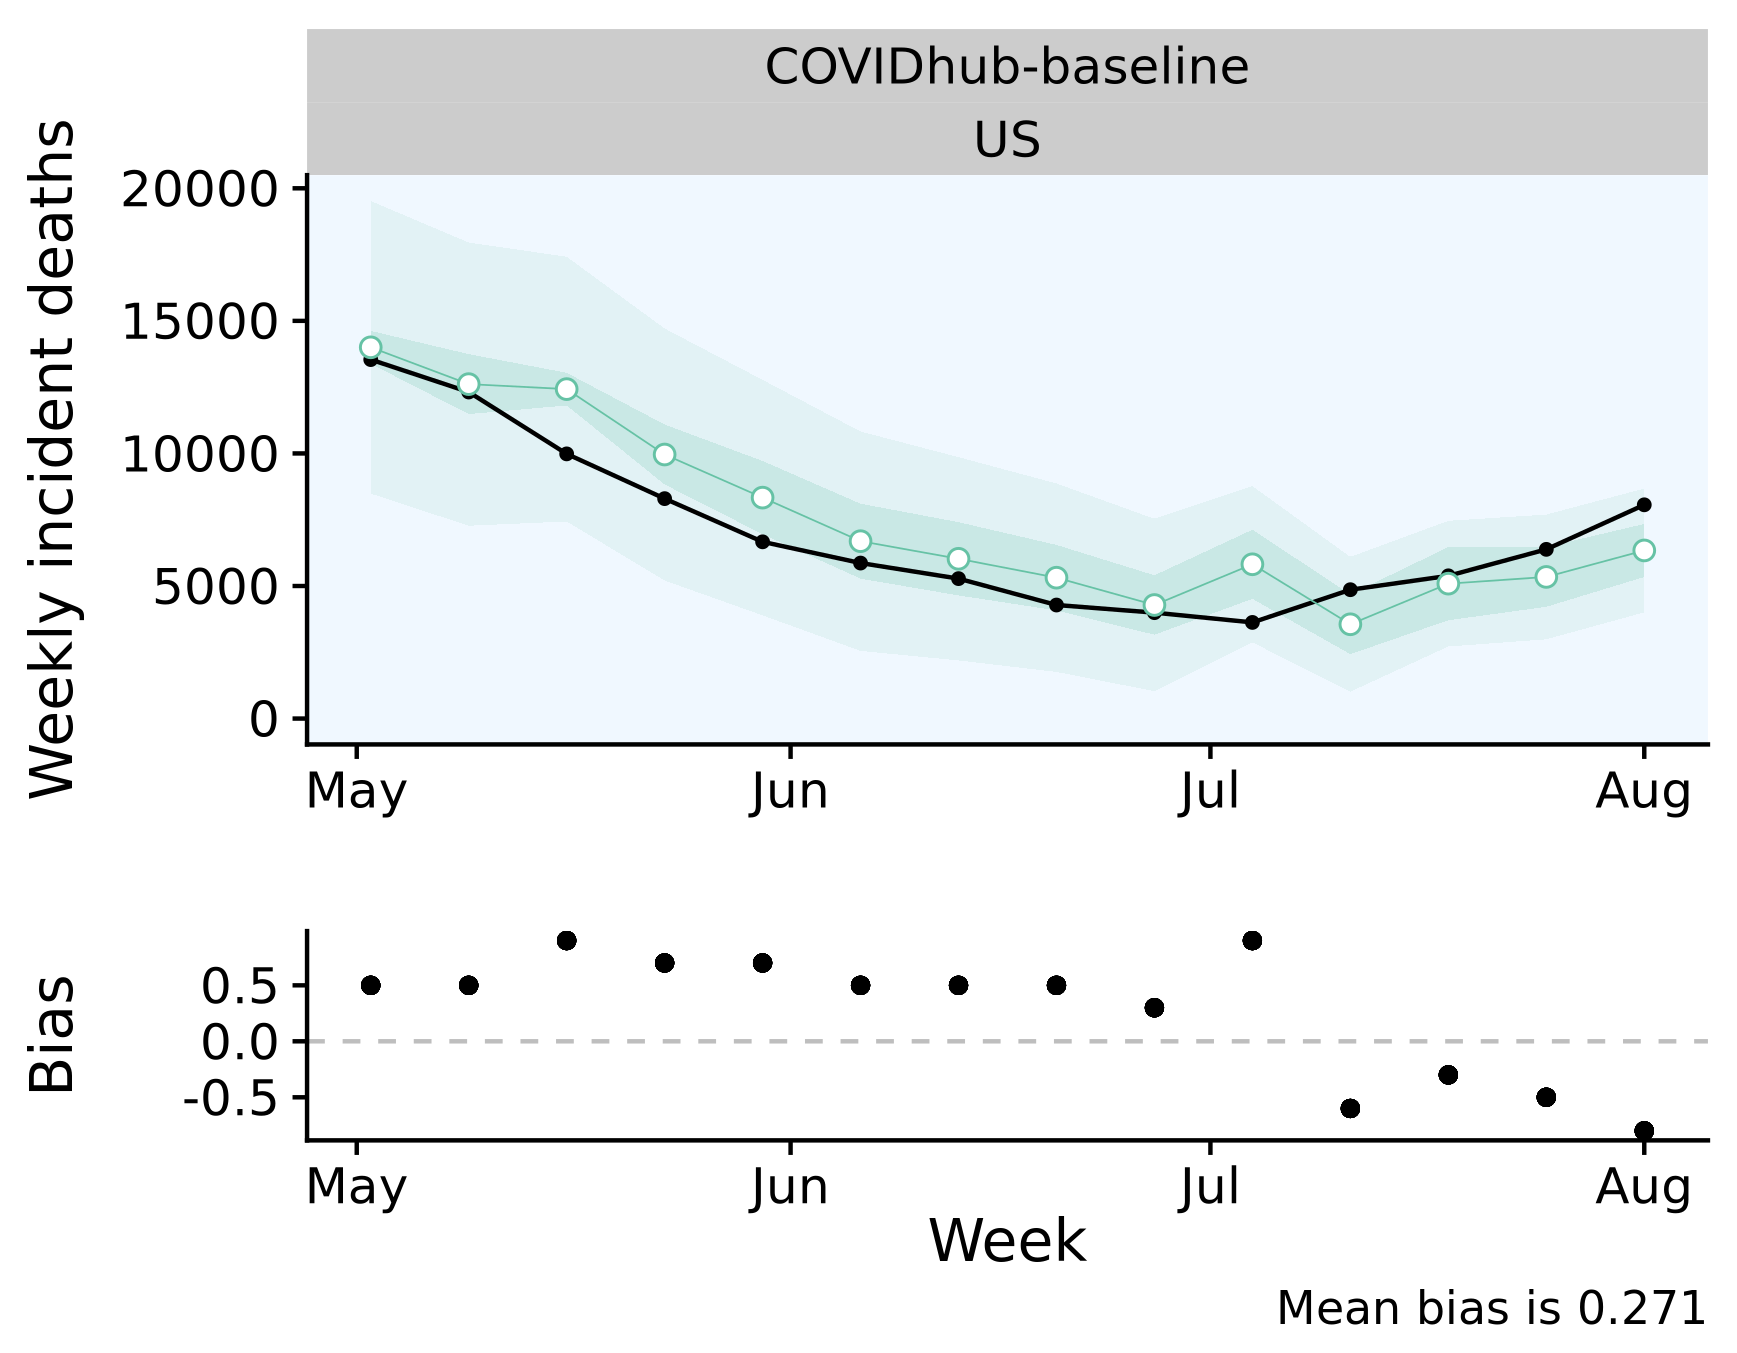
\includegraphics[width=1\linewidth]{../visualisation/chapter-3-evaluation/bias_example} \caption{One week ahead forecasts from the COVIDhub-baseline model for the US (top) and corresponding bias values (bottom)}\label{fig:bias-example}
\end{figure}

\hypertarget{calibration-and-empirical-coverage}{%
\subsection{Calibration and empirical coverage}\label{calibration-and-empirical-coverage}}

Another way to look at calibration (precisely: probabilistic calibration in \citet{gneitingProbabilisticForecastsCalibration2007}) is to compare empirical coverage of observed values with the nominal coverage implied by the CDF of the predictive distribution. This is most easily understood in the context of quantile forecasts, but can in principle be transferred to continuous and integer forecasts as well.

To assess empirical coverage at a certain interval range, we simply measure the proportion of true observed values that fall into corresponding range of the predictive distribution. If the 0.05, 0.25, 0.75, and 0.95 quantiles are given, then 50\% of the true values should fall between the 0.25 and 0.75 quantiles and 90\% should fall between the 0.05 and 0.95 quantiles. We can calculate and plot these values to inspect how well different interval ranges of the forecast are calibrated. This is illustrated in the left plot in Figure \ref{fig:coverage} where the empirical coverage of the US forecasts of the COVIDhub-baseline model is shown. We can seen that the interval coverage for the outer prediction intervals looks reasonable, but inner prediction intervals seem to miss too many observations.

\begin{figure}
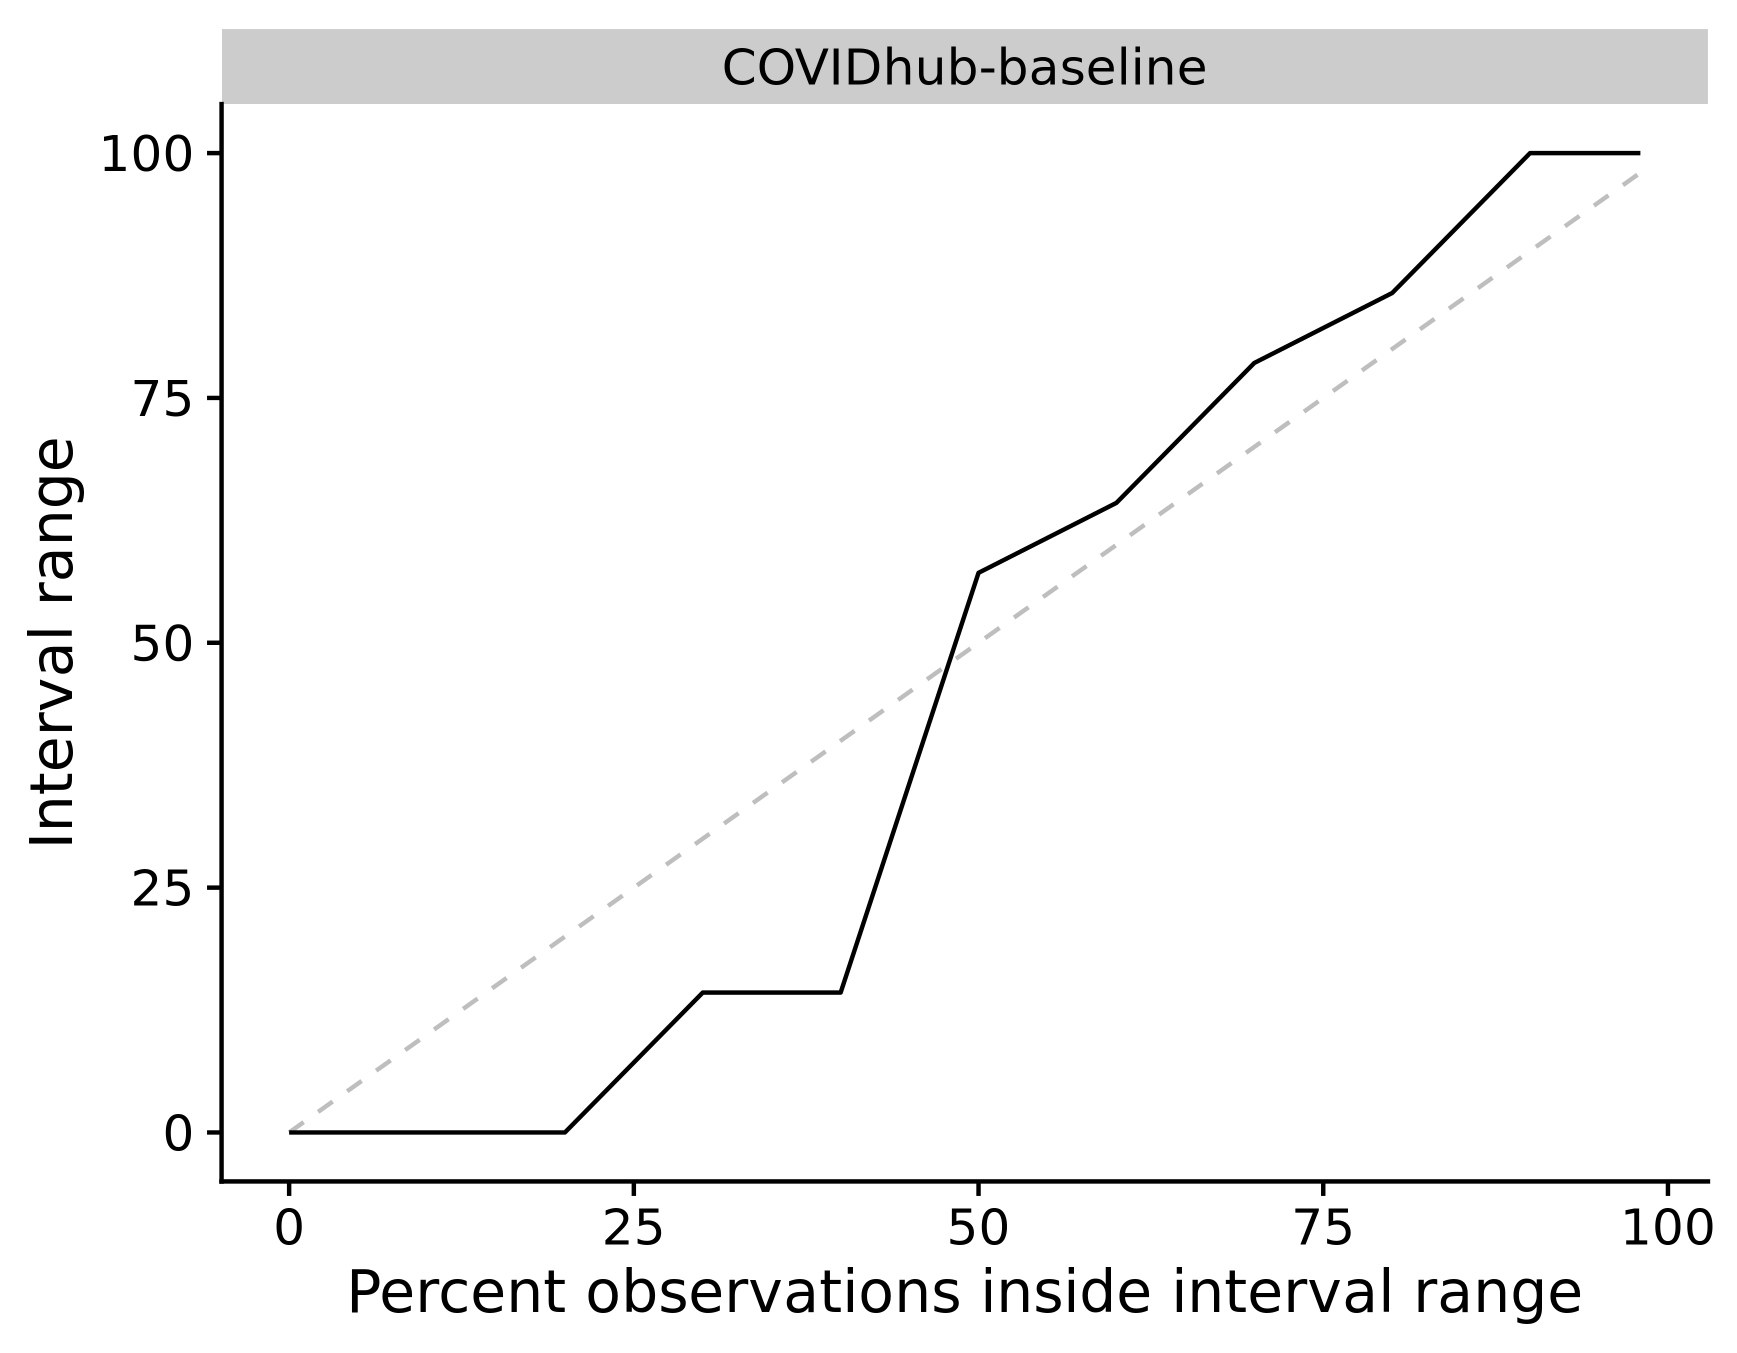
\includegraphics[width=0.5\linewidth]{../visualisation/chapter-3-evaluation/interval-coverage} 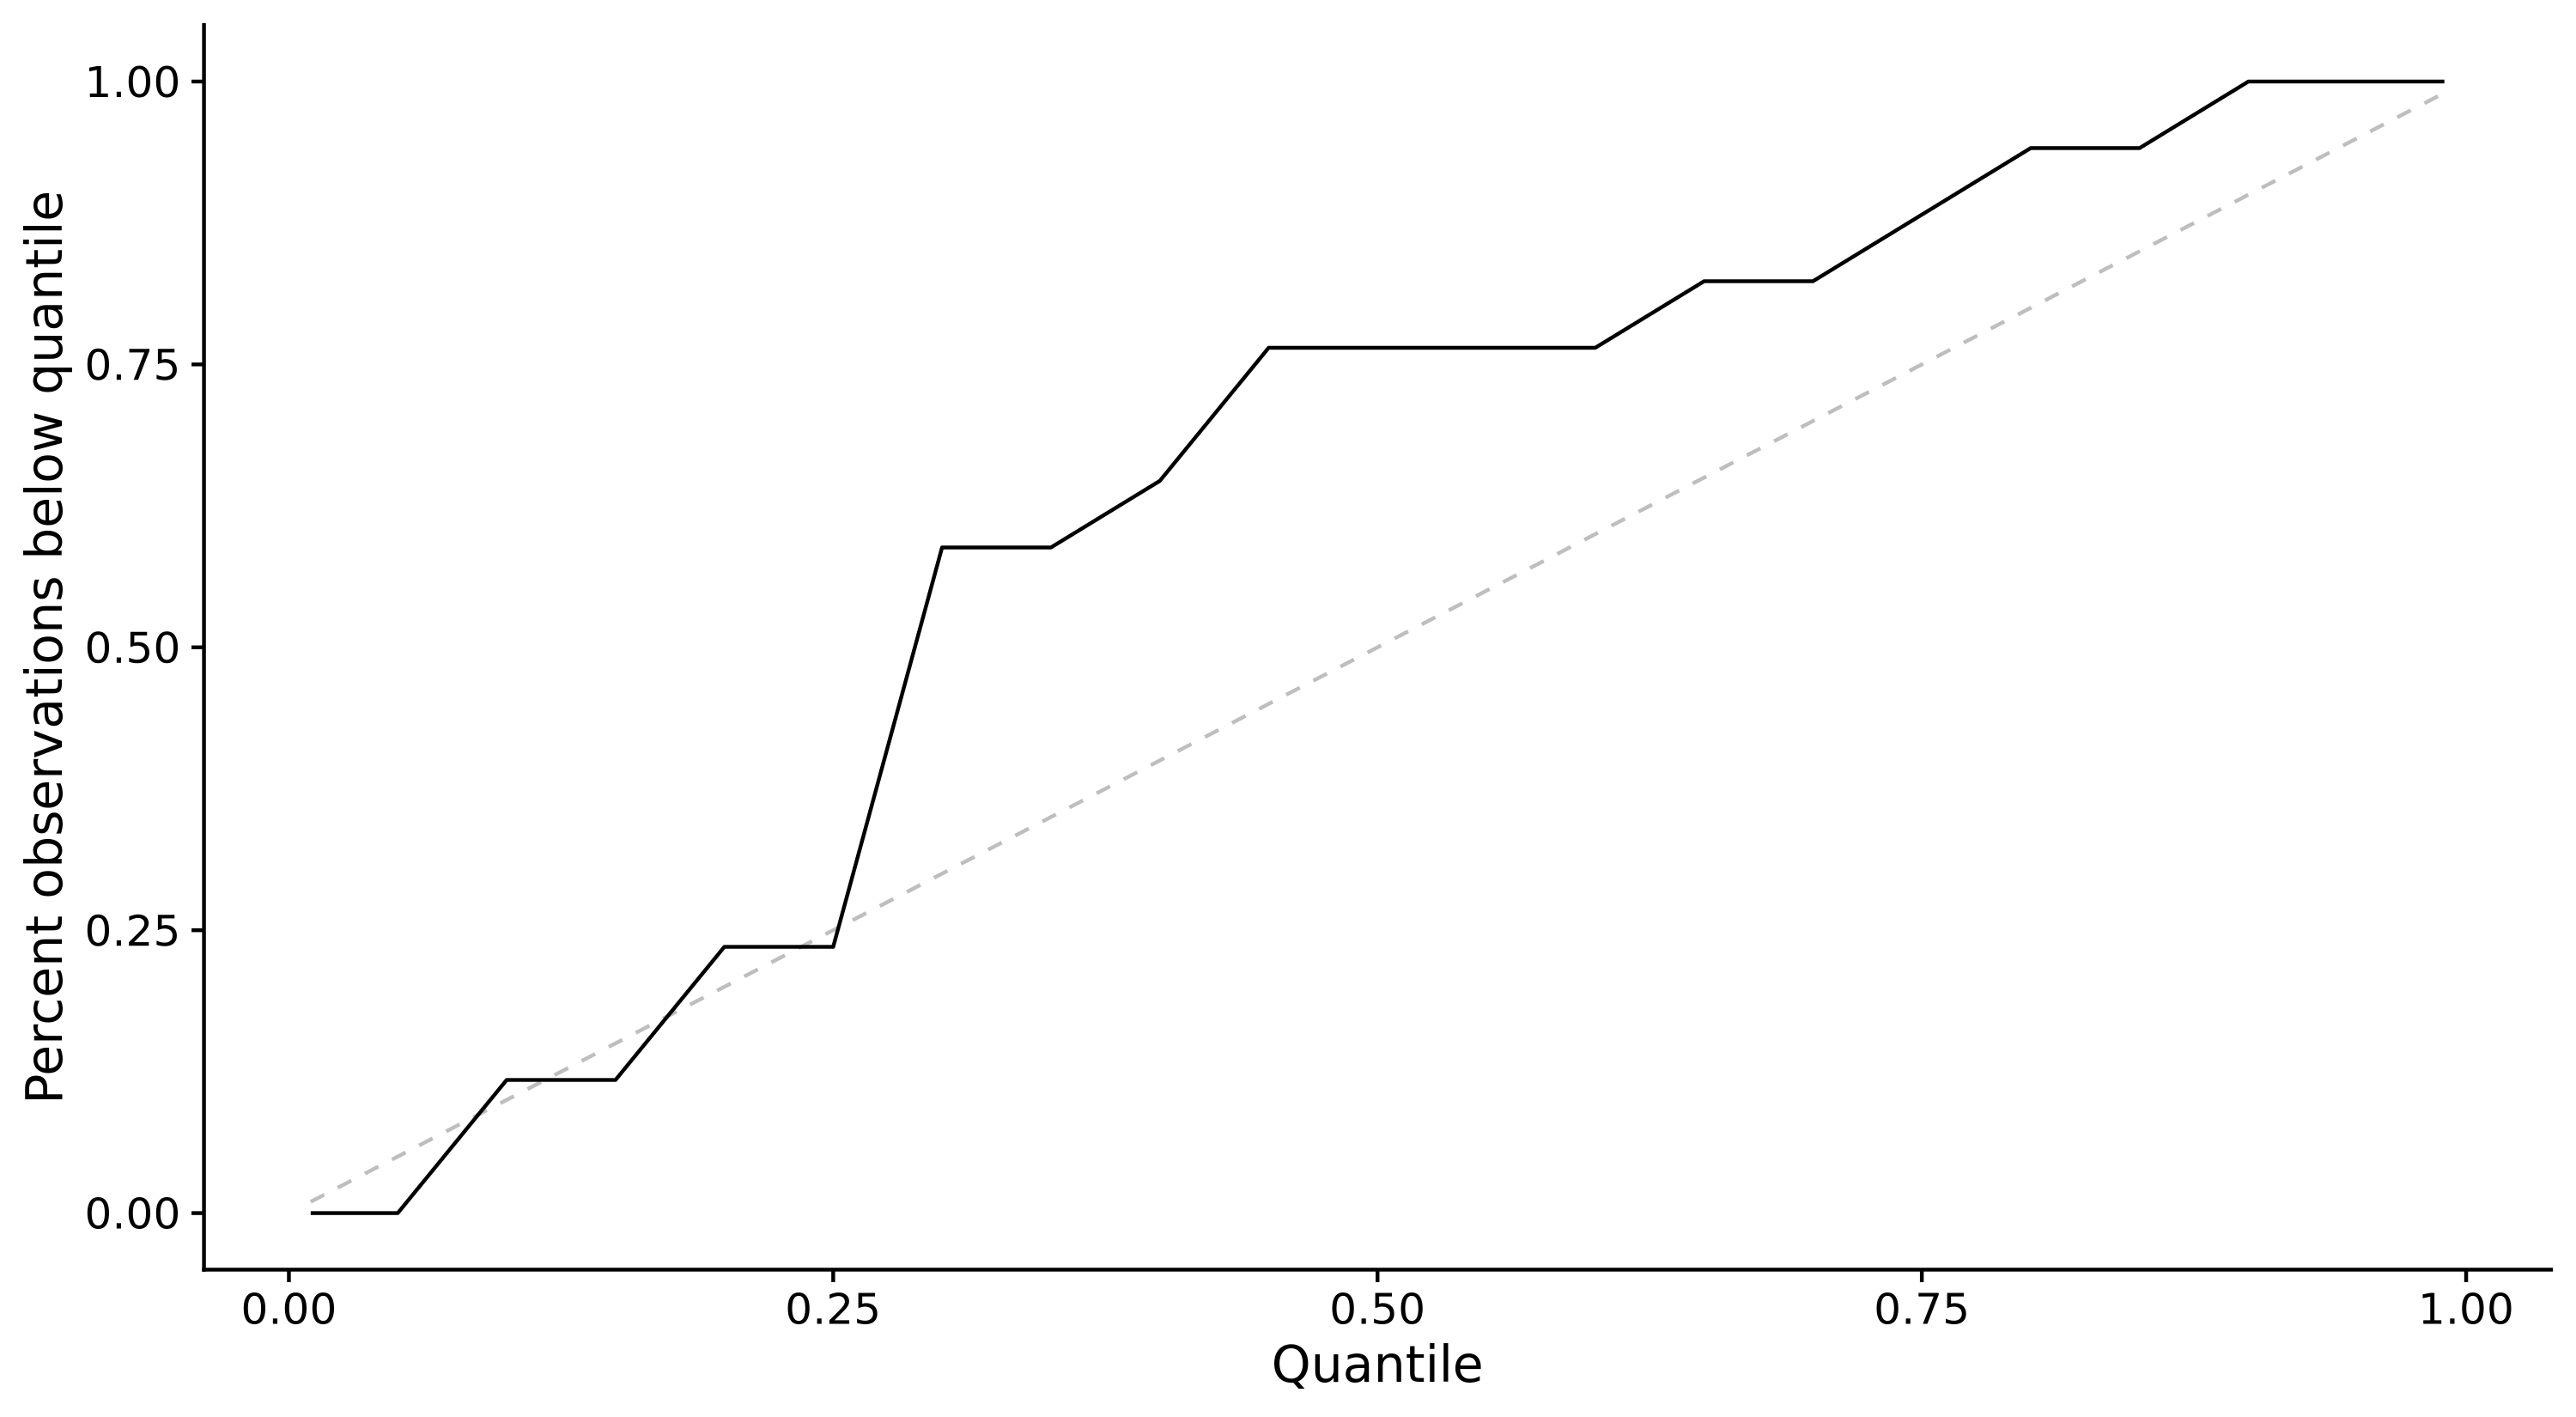
\includegraphics[width=0.5\linewidth]{../visualisation/chapter-3-evaluation/quantile-coverage} \caption{Empirical coverage of prediction intervals (left) quantiles of the predictive distribution (right) for one week ahead forecasts from the COVIDhub-baseline model.}\label{fig:coverage}
\end{figure}

To get an even more precise picture, we can also look at the percentage of true values below every single quantile of the predictive distribution. This is shown on the right in Figure \ref(fig:coverage). This plot suggests that the miscalibration largely comes from an upward bias of the inner prediction interval. The major problem to address then, it seems, is not necessarily the general width of the prediction intervals, but foremost the upward bias of the inner quantiles.

\hypertarget{calibration-and-the-probability-integral-transform}{%
\subsection{Calibration and the probability integral transform}\label{calibration-and-the-probability-integral-transform}}

As explained earlier, the CDF of predictice distribution \(P_t\) should ideally be equal to the CDF of the true unknown distribution \(F_t\) that generated the observed value \(x_t\). In order to assess whether there are substantial deviations between the two, \citet{dawidPresentPositionPotential1984} suggested to transform the observed values using the predictive distribution. The idea is then to
check whether the probability integral transform (PIT) of the observed values follows a uniform distribution. The PIT is given by

\[u_t = P_t (x_t)\]
where \(u_t\) is the transformed variable and \(P_t(x_t)\) is the predictive distribution evaluated at the true observed value \(x_t\). If \(P_t = F_t\) at all times \(t\), then \(u_t, t = 1 \dots T\) will follow a uniform distribution (for a proof see e.g.~\citet{angusProbabilityIntegralTransform1994}).

In the case of discrete outcomes, the PIT is no longer uniform even when forecasts are ideal. As \citet{funkAssessingPerformanceRealtime2019} suggest, we can instead use a randomised PIT instead by redefining \[u_t = P_t(x_t) + v \cdot (P_t(x_t) - P_t(x_t - 1) )\]
where \(x_t\) is again the observed value at time \(t\), \(P_t()\) is the CDF of the predictive distribution function and \(P_t (-1) = 0\) by definition. \(v_t\) is a standard uniform variable and independent of \(x_t\). If \(P_t\) is equal to the true data-generating distribution function, then \(u_t\) is standard uniform. \citep{czadoPredictiveModelAssessment2009} also propose a non-randomised version of the PIT for count data that could be used alternatively.

One can then plot a histogram of \(u_t\) values to look for deviations from uniformity. U-shaped histograms often result from predictions that are too narrow, while hump-shaped histograms indicate that predictions may be too wide. Biased predictions will usually result in a triangle-shaped histogram. Figure \ref{fig:pit-examples} shows four different simulated example PIT histograms that illustrate these characteristics.

\begin{figure}

{\centering 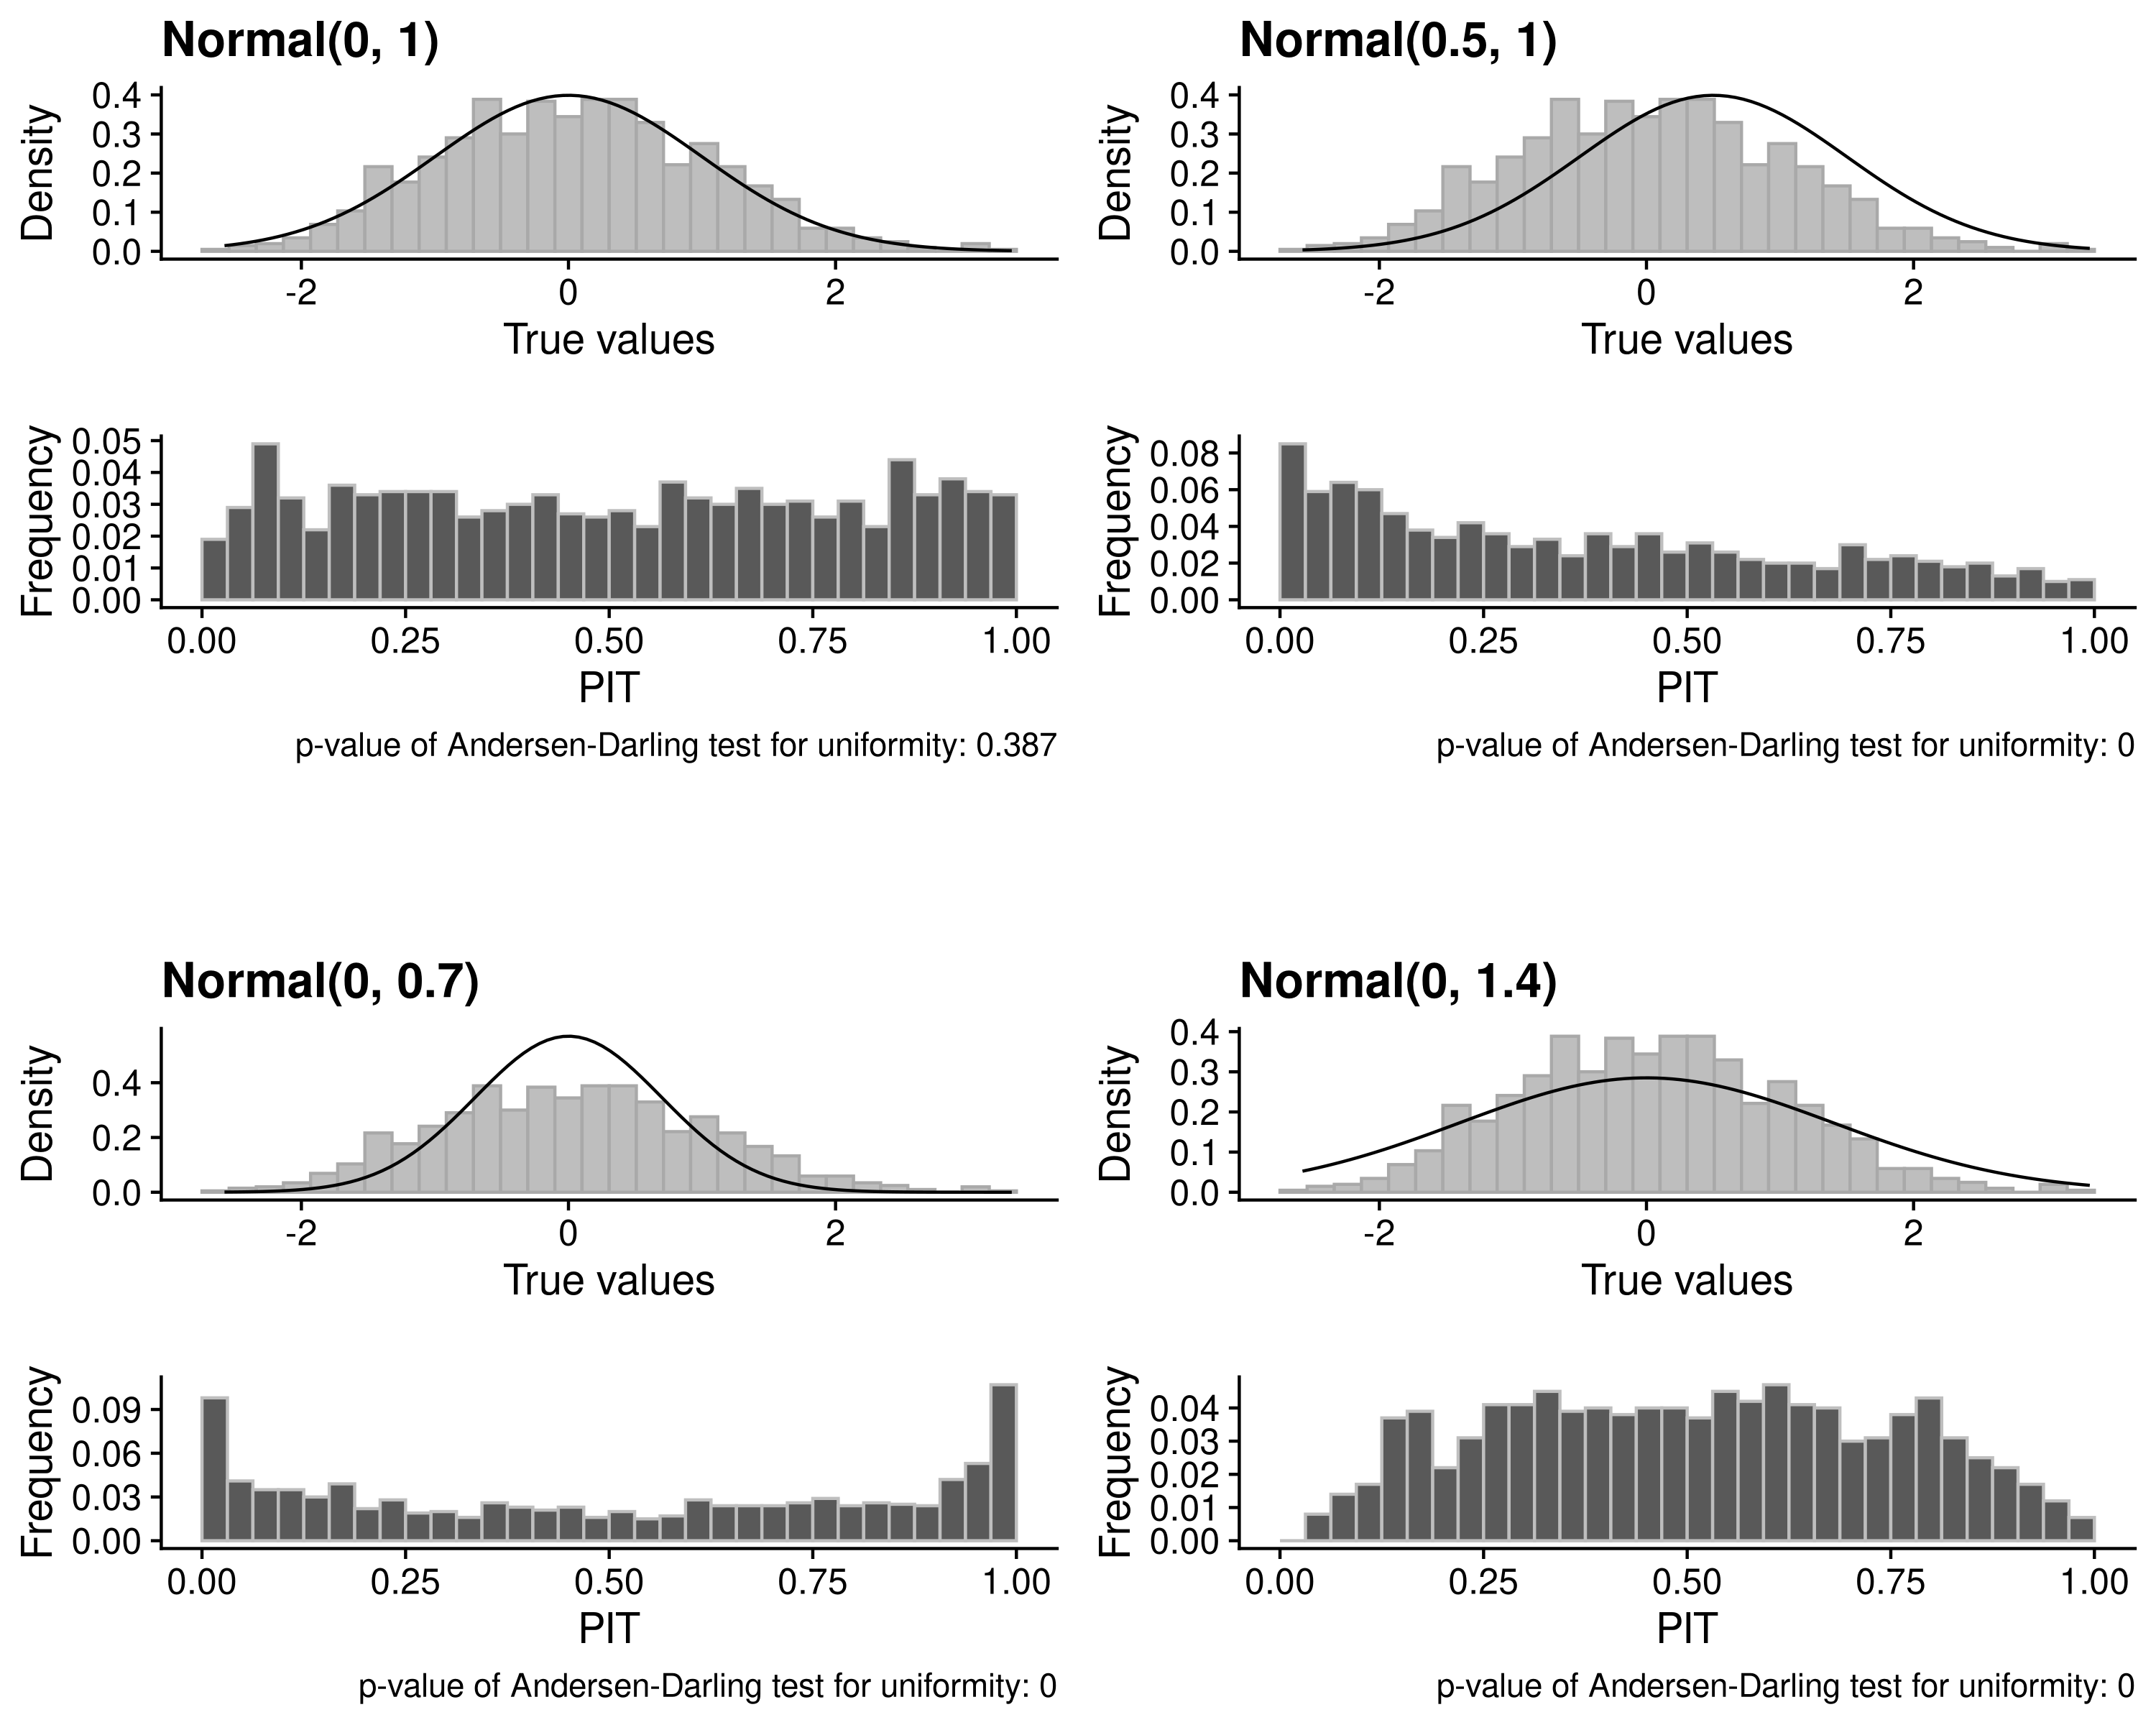
\includegraphics[width=1\linewidth]{../visualisation/chapter-3-evaluation/calibration-examples} 

}

\caption{Four examples of different predictive distributions and the correspoding PIT histograms below. The data always follows the same Normal(0,1) distribution. Preditive distributions are indicated by the title of the subplot.}\label{fig:pit-examples}
\end{figure}

In addition to the visual inspection, \citet{funkAssessingPerformanceRealtime2019} suggest to apply an Anderson-Darling \citep{andersonAsymptoticTheoryCertain1952} test for uniformity to the transformed values. The test cannot prove uniformity, but only assess whether there is evidence against it. As a rule of thumb, Funk et al.~suggest there is no evidence to call a forecasting model miscalibrated if the p-value found was greater than a threshold of \(p \geq 0.1\), some evidence that it is miscalibrated if \(0.01 < p < 0.1\), and good evidence that it is miscalibrated if \(p \leq 0.01\). The test seems rather conservative though\footnote{As evidence, we present the results of a small simulation study with i = 1 000 iterations. For every iteration, n = 1 000 true values were simulated. Everyone of these true values was `predicted' using s = 10 000 samples from the same standard normal distribution. For each set of true values and predictions, the probability integral transform was applied followed by the Anderson-Darling test for uniformity. Out of 1000 iterations, there were 165 p-values \(\leq 0.01\), 88 p-values \(0.01 < p < 0.1\) and 747 p-values \(\leq 0.01\). Note that 1000 true values is quite high for many applied settings. For n = 100 true\_values and s = 2000 samples, the result was 108, 87 and 805. We can conclude that the AD test may be prone to reject a meaningful fraction of well calibrated predictions.}

\citet{hamillInterpretationRankHistograms2001} discusses in length that uniformity of the PIT histogram is a necessary, but not a sufficient condition for calibration. Nevertheless, the PIT histogram can give us a good impression of the reliability of our forecasts. Figure \ref{fig:pit-baseline-model} shows the pit histogram for one-week-ahead predictions made by the COVIDhub-baseline model across different states. We can see that the PIT histogram presents a pattern that suggests under-dispersion may be present, i.e.~at least some of the confidence intervals may be too narrow. This corresponds well to the observation made in the coverage plot in Figure \ref{fig:coverage}.

\begin{figure}
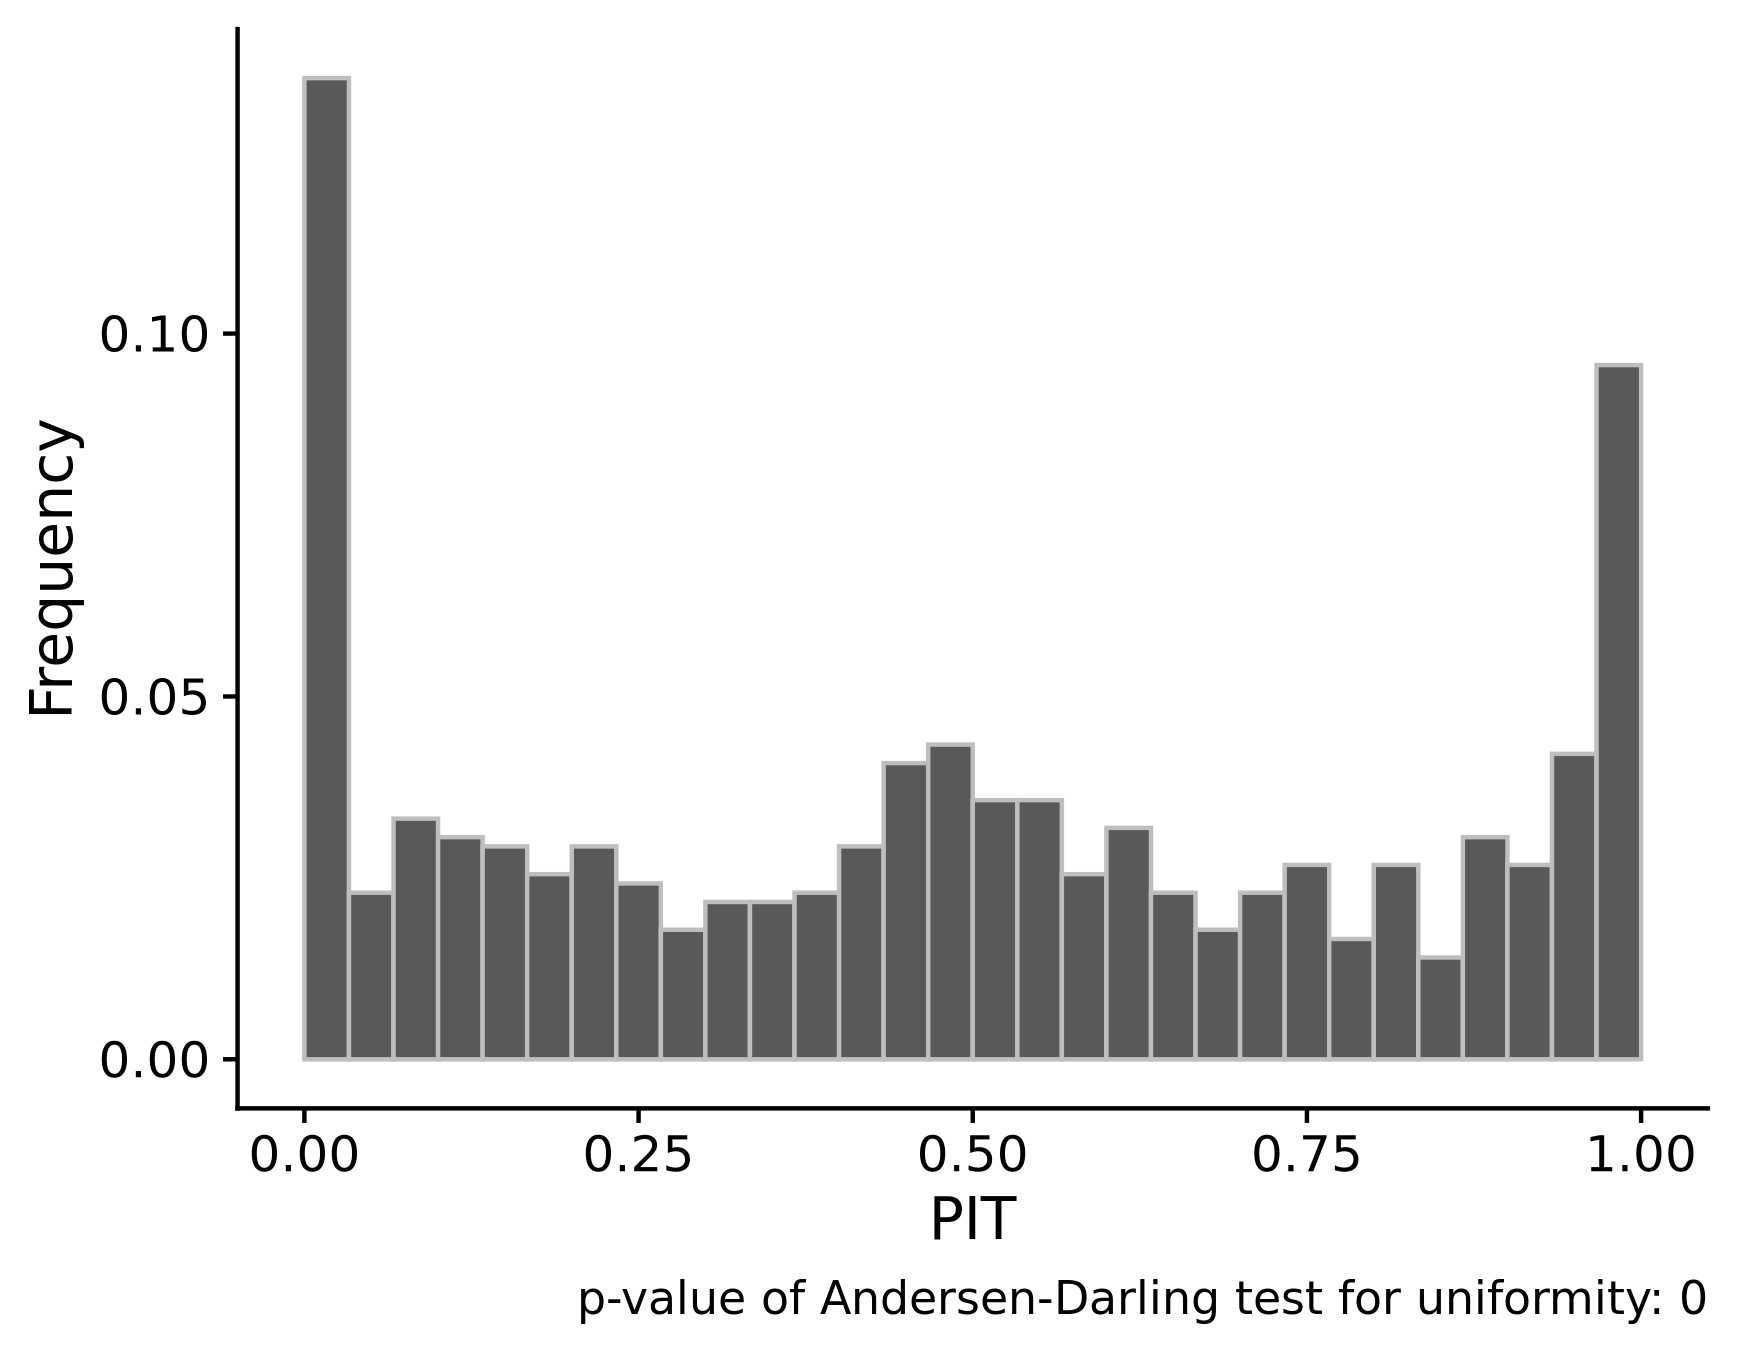
\includegraphics[width=1\linewidth]{../visualisation/chapter-3-evaluation/pit-baseline-model} \caption{PIT histogram for one-week-ahead forecasts from the COVIDhub-baseline model. In order to obtain samples, a separate gamma distribution was first fit to every set of quantiles provided to the Forecast Hub using the `nloptr` package [@R-nloptr]. Samples were then drawn from these distributions. We can see a pattern commonly found in underdispersed predictions}\label{fig:pit-baseline-model}
\end{figure}

After having looked at calibration, we can now turn to sharpness, the second aspect central to model evaluation.

\hypertarget{assessing-sharpness}{%
\section{Assessing sharpness}\label{assessing-sharpness}}

Sharpness, i.e.~the ability to produce narrow forecasts, is a quality of the forecasts only and does not depend on the observations. Sharpness is therefore only of interest conditional on calibration: a very precise forecast is not useful if it is clearly wrong. Again we need to take slightly different approaches for continuous, integer and quantile forecasts. For continuous and integer forecasts we follow the suggestion from \citet{funkAssessingPerformanceRealtime2019}. For quantile forecasts we propose a novel metric.

For continuous and integer forecasts, \citet{funkAssessingPerformanceRealtime2019} suggest to measure sharpness as the normalised median absolute deviation about the median (MADN), i.e.~

\[ S_t(P_t) = \frac{1}{0.675} \cdot \text{median}(|y - \text{median(y)}|) \],

where \(y\) is the vector of all predictive samples and \(\frac{1}{0.675}\) is a normalising constant that ensures that sharpness will equal the standard deviation of the predictive distribution if \(P_t\).

For quantile forecasts, we propose to measure sharpness as a weighted mean of the width of the interval ranges. Let \(Q_t\) be a set of predicted quantiles for a true \(x_t\) at time \(t\). This set of quantiles is assumed to be symmetric, such that there always exist corresponding elements \(q_{t, \frac{\alpha}{2}}\) and \(q_{t, 1-\frac{\alpha}{2}}\). These corresponding pairs of quantiles cover a \((1 - \alpha) \cdot 100\) interval range. We measure the sharpness of a quantile forecast at time \(t\) as

\[\text{sharpness}_t = \sum_{\alpha} \frac{\alpha}{2} (q_{t, 1 - \frac{\alpha}{2}} - q_{t, \frac{\alpha}{2}}) \].

The width of prediction intervals is a natural way to measure the sharpness of a predictive distribution. Weighting the width of different intervals with \(\frac{\alpha}{2}\) ensures that the score does not grow indefinitely for very large prediction intervals (and correspondingly, very small \(\alpha\)). We also argue that \(\frac{\alpha}{2}\) is a natural choice for a weight as it corresponds to the weight most commonly used in the weighted interval score described in the next section.

\hypertarget{proper-scoring-rules}{%
\section{Proper scoring rules}\label{proper-scoring-rules}}

Instead of assessing calibration and sharpness independently, we can make use of proper scoring rules to express the quality of our forecast in a single number. Propriety is a feature of a score that guarantees that the ideal forecast will always receive the lowest score \citep{gneitingStrictlyProperScoring2007}. A forecaster judged by a proper scoring rule is therefore always incentivised to make forecasts as close to the true data-generating distribution as possible. In the following, three proper scoring rules will be presented.

MAYBE EXPLANATION OF SEPARATION OF PROPER SCORING RULES INTO CALIBRATION AND SHARPNESS PART? HANS HERSBACH?

\hypertarget{log-score}{%
\subsection{Log Score}\label{log-score}}

The Log score is probably the oldest proper scoring rule and can be traced back to \citet{shannonMathematicalTheoryCommunication1948} and his work on communication and information theory and to \citet{goodRationalDecisions1952} who first proposed a log score for binary predictions. The Log Score is now widely used in all sorts of fields, especially in Bayesian inference (see e.g.~\citep{gelmanUnderstandingPredictiveInformation2014}). The log score is simply the log density of the predictive distribution at time \(t\) evaluated at the true observed value, i.e.~

\[ \text{log score}_t = \log p_t(x_t)\]
where \(p_t\) is the predictive density function at time \(t\). This is illustrated in Figure \ref{fig:log-score}. In this formulation, larger values are better, but one can of course simply reverse the sign. One problem with the log score is that it can be quite unstable for values of \(p_t(x_t)\) close to zero. The log score will therefore not play a large role in this thesis, but is mentioned for completeness sake as it of great importance to many applications. It also illustrates the concept of looking at observations in terms of the predictive distribution quite nicely.

\begin{figure}
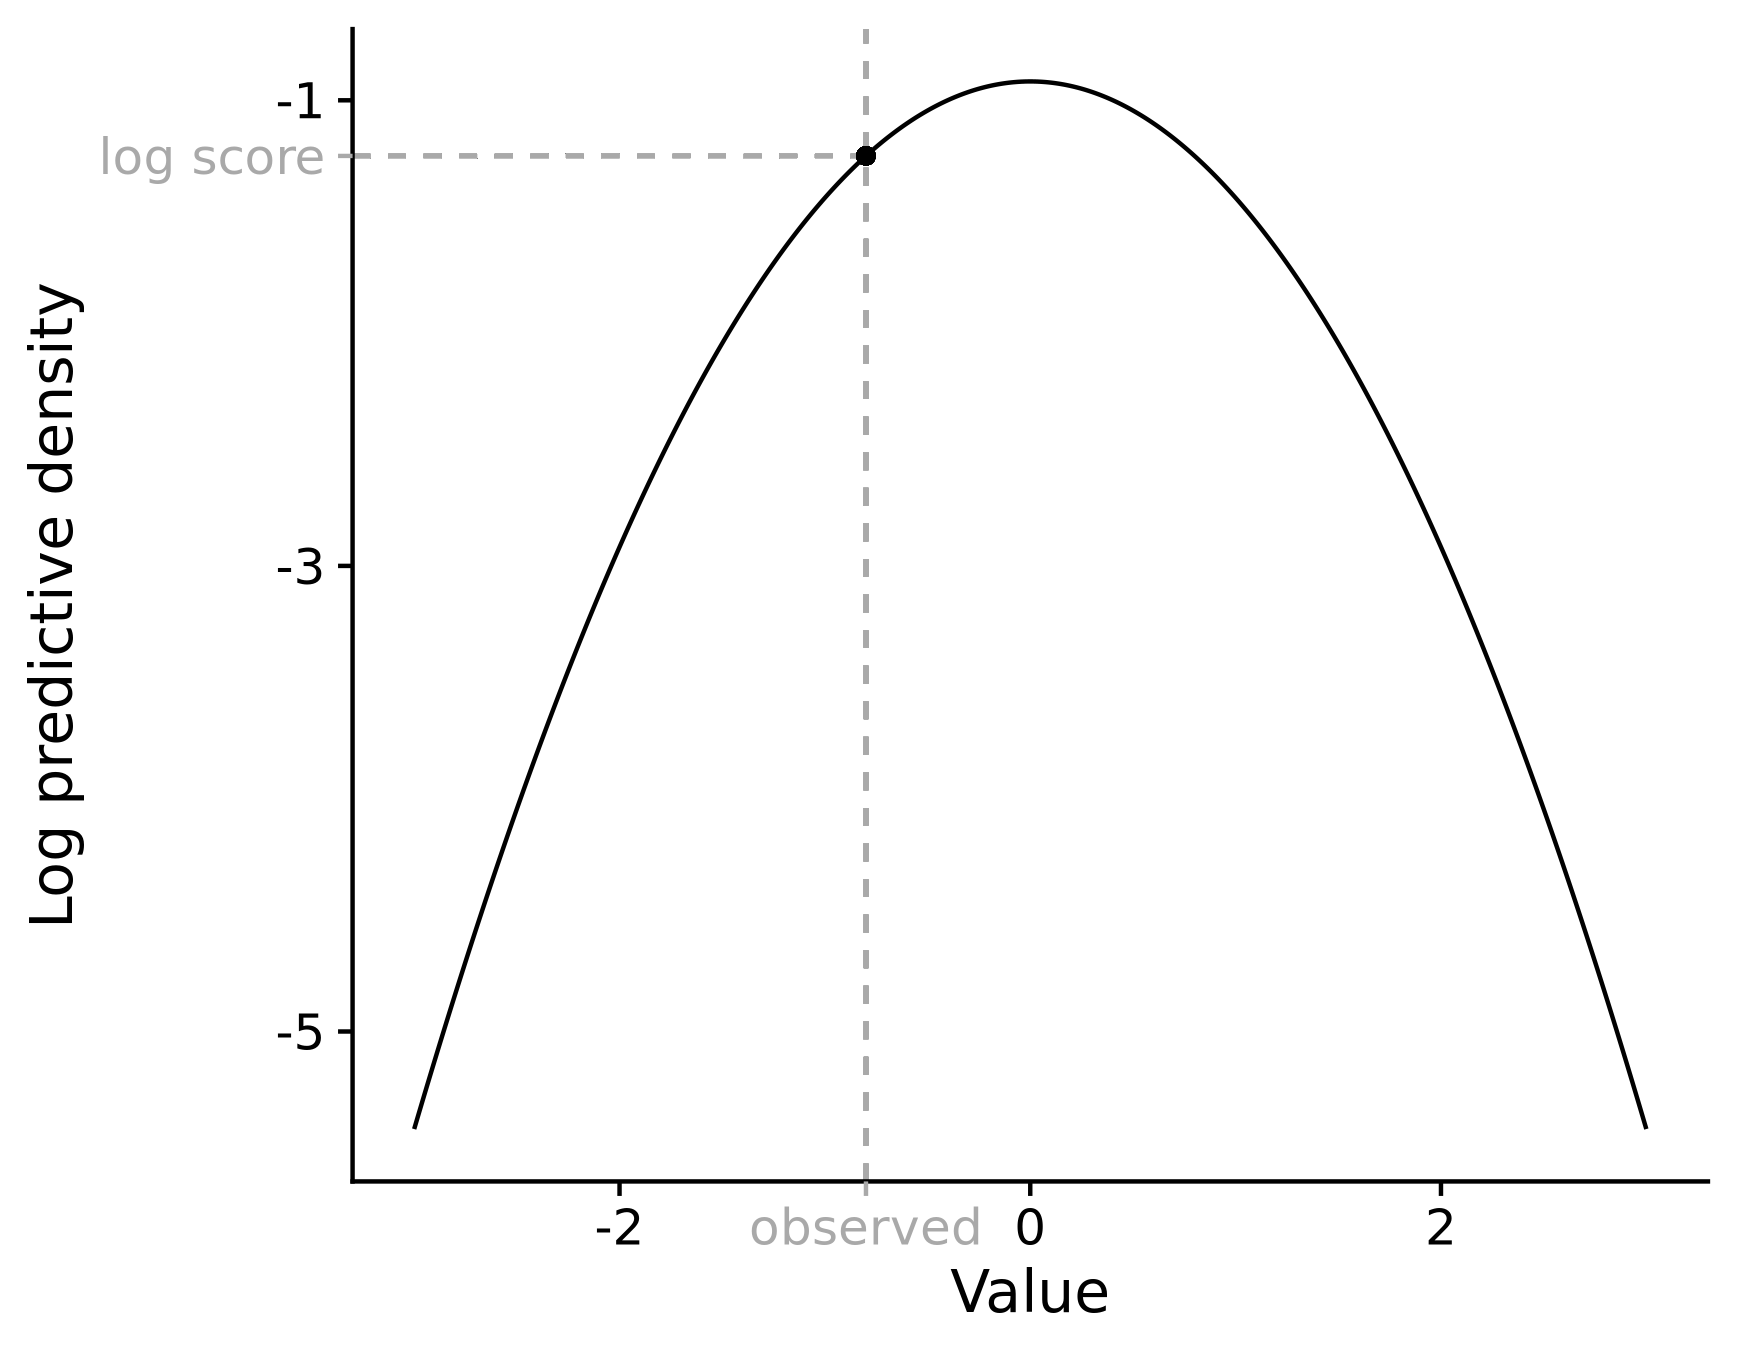
\includegraphics[width=1\linewidth]{../visualisation/chapter-3-evaluation/log-score-example} \caption{Illustration of the Log score as the log predictive desnity evaluated at the true observed value}\label{fig:log-score}
\end{figure}

\hypertarget{continuous-ranked-probability-score}{%
\subsection{(Continuous) Ranked Probability Score}\label{continuous-ranked-probability-score}}

THIS SECTION COULD BE FORMULATED SLIGHTLY NICER. MAYBE START WITH THE PART THAT WE MEASURE THE DISTANCE BETWEEN CDF AND PREDICTIVE DISTRIBUTION.

The Continuous Ranked Probability Score (CRPS) \citep{mathesonScoringRulesContinuous1976, gneitingStrictlyProperScoring2007} is another proper scoring rule that is considered more stable and therefore better suited for our purposes. The CRPS is defined as

\begin{equation}
\label{eq:crps}
\text{CRPS}(P_t, x_t) = \int_{-\infty}^\infty \left( P(y) - \mathbb(1)(y \geq x_t) \right)^2 dy,
\end{equation}

where \(P_t\) is again the CDF of the predictive distribution and \(x_t\) is the true observed value.

The CRPS can also be expressed as

\[ \text{CRPS}(P_t, x_t) = \frac{1}{2} \mathbb{E}_{P_t} |X - X'| - \mathbb{E}_P |X - x_t| \],

where \(X\) and \(X'\) are independent realisations from the predictive distributions \(P_t\) with finite first moment (\citet{gneitingStrictlyProperScoring2007}). This formulation is convenient as we can simply replace \(X\) and \(X'\) with predictive samples and sum over all possible combinations to obtain the desired sample CRPS.

For integer counts, we can use the Ranked Probability Score (RPS) as proposed by \citet{epsteinScoringSystemProbability1969} and \citet{murphyRankedProbabilityScore1969}, and discussed e.g.~by \citet{czadoPredictiveModelAssessment2009}. The RPS is defined as

\[ \text{rps}(P_t, x_t) = \sum_{y = 0}^\infty (P_t(y) - \mathbb(1) (y \geq x_t))^2 \]

Smaller values of the (C)RPS are preferable. For the case of a point prediction, the predictive distribution degenerates to a distribution with its entire masss on the single predicted point. In this case, the CRPS is equivalent to the mean absolute error (MAE) of the point prediction. If we consider Equation \eqref{eq:crps} for a step function, then the crps will equal the area between the true observed value and the predicted value (as \(1^2 = 1\) and the height of the rectangle is again 1).
This is illustrated in the top half of Figure \ref{fig:crps-explanation}. For other distributions this will not hold, as \(P_t()\) is in Equation \eqref{eq:crps}. Intuitively, we can nevertheless understand the CRPS as measuring the vertical distance between the predictive CDF and the true value as illustrated in the bottom half of Figure @ref(crps\_explanation),

\begin{figure}
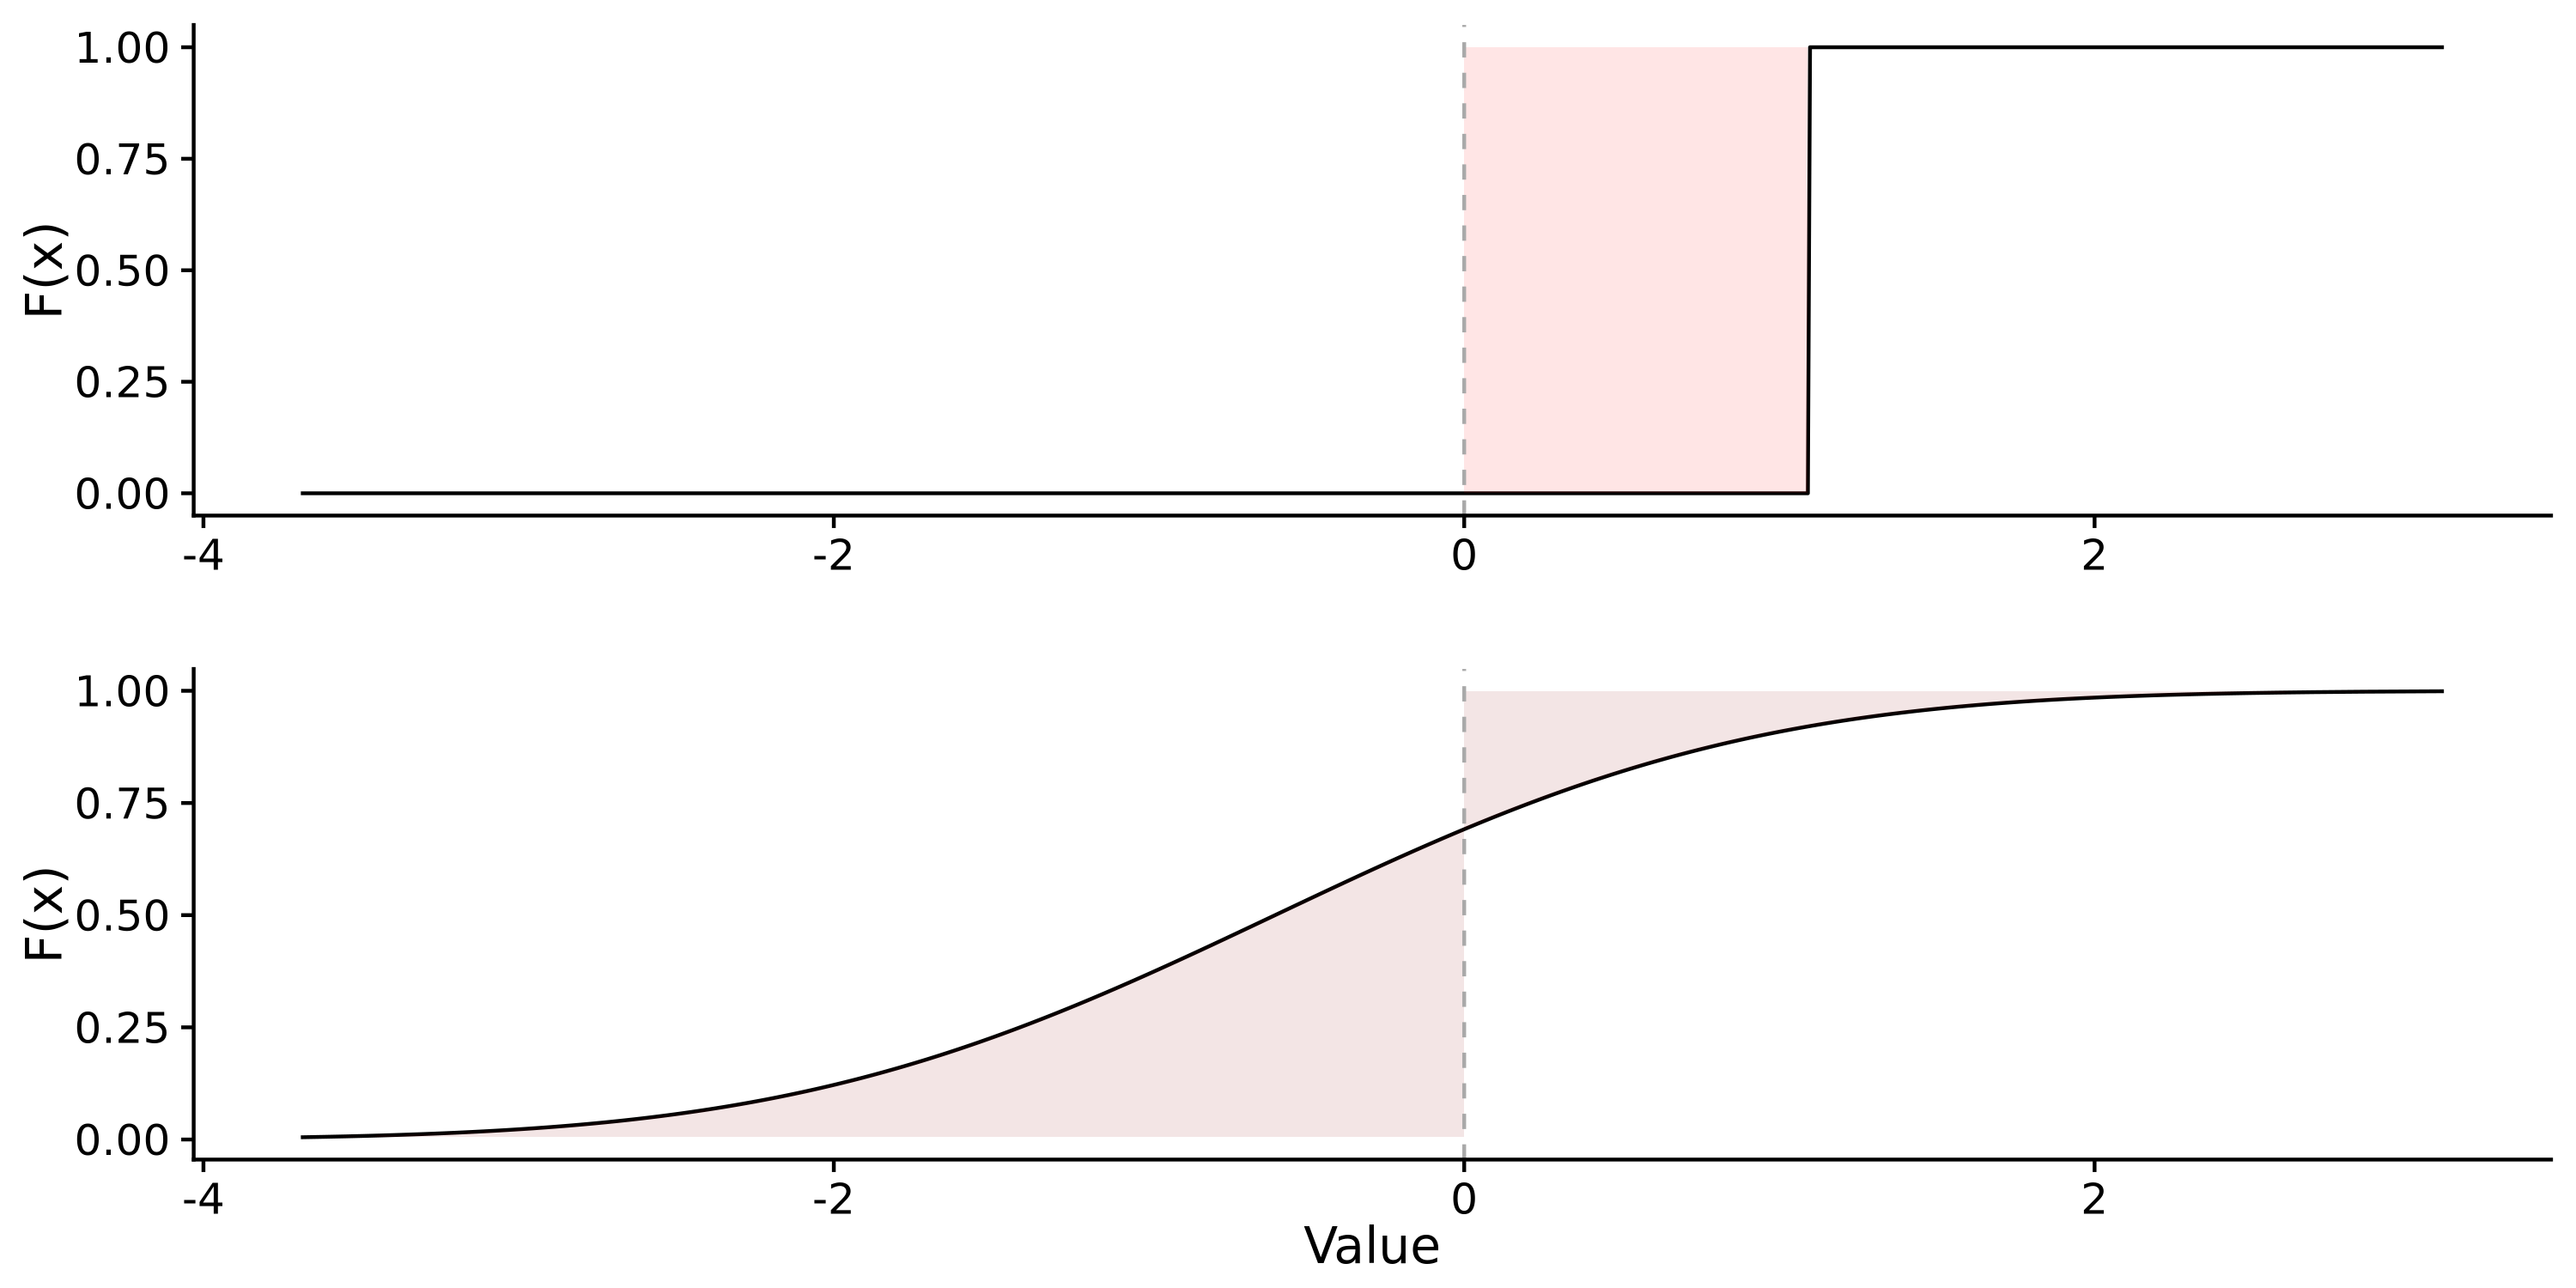
\includegraphics[width=1\linewidth]{../visualisation/chapter-3-evaluation/crps-explanation} \caption{Illustration of the CRPS. Top: CRPS for a predictive distribution with point mass on the predicted value, $1$. The CRPS corresponds to the mean absolute error of the point prediction, i.e. the absolute difference between the predicted value 1 and the true observed value 0. Bottom: Intuitive llustration of the CRPS as the vertical distance between the CDF and the true value. Note that the CRPS does not in fact equal the shaded area, as the term in @
ef(eq:crps) is squared.}\label{fig:crps-explanation}
\end{figure}

\hypertarget{interval-score}{%
\subsection{Interval score}\label{interval-score}}

The Interval Score is a proper scoring rule to evaluate predictions in a quantile format \citep{bracherEvaluatingEpidemicForecasts2020, gneitingStrictlyProperScoring2007}. Let us consider a pair of predictive quantiles \(q_{\frac{\alpha}{2}}, q_{1-\frac{\alpha}{2}}\) that form a \((1 - \alpha) * 100\) prediction interval. Let us denote \(q_{\frac{\alpha}{2}}\), the lower bound, as \(l\), and \(q_{1-\frac{\alpha}{2}}\), the upper bound, as \(u\). Then the Interval score is given as

\[\text{IS}_{\alpha} = (u - l) + \frac{2}{\alpha} \cdot (l - x) \cdot \mathbb{1}(x \leq l) 
+ \frac{2}{\alpha} \cdot (x - u) \cdot \mathbb{1}(x \geq u)\]

This score can be separated into three parts: \((u - l)\) measures the sharpness of the predictive distribution. \(\frac{2}{\alpha} \cdot (l - x) \cdot \mathbb{1}(x \leq l)\) and \(\frac{2}{\alpha} \cdot (x - u) \cdot \mathbb{1}(x \geq u)\) are penalties that occur if the observed value falls below the lower or above the upper end of the interval range. Smaller values of the interval scores are preferred.

Usually, more than one predictive interval is reported at once. We can obtain the overall interval score as a (weighted) sum of individual interval score contributions:

\[ \text{IS} = \sum_\alpha w_\alpha \cdot \text{IS}_\alpha\].

This interval score is proper for any non-negative choice of \(w_\alpha\). For \(w_\alpha = \frac{\alpha}{2}\), one can show that the interval score converges to the CRPS for an increasing set of equally spaced prediction intervals \citep{bracherEvaluatingEpidemicForecasts2020} MAYBE MORE REFERENCES FROM THE PAPER. We shall call the so weighted score the weighted interval score (WIS).

PART THAT WIS FOR ALPHA = 1 IS PROPORTIONAL TO THE MAE

\hypertarget{a-proposed-evaluation-framework}{%
\section{A proposed evaluation framework}\label{a-proposed-evaluation-framework}}

The previous sections have introduced a variety of different metrics that can help to highlight different important aspects of model performance. Based on these individual building blocks we propose the following structured approach to model evaluation:

\begin{enumerate}
\def\labelenumi{\arabic{enumi}.}
\tightlist
\item
  Visualise the observed data as well as the predictions to get a feeling for how individual models perform. Revisit these plots at each step of the evaluation process.
\item
  Calculate summarised scores for all metrics and proper scoring rules to obtain a ranking of the different models and a rough indicator of potential problems. Break down scores by aggregating over different subgroups of the data like locations, dates or forecast horizons.
\item
  Examine calibration and sharpness in detail. This includes examining PIT histograms and plots for bias, coverage and sharpness, broken down again by different subgroups. This analysis can provide important feedback for model improvement and help to avoid possible pitfalls hidden by the aggregated scores.
\item
  Use a regression framework to help with model selection and determine significant differences between model performance. We propose estimating a mixed-effects model with the chosen proper scoring rule as the dependent variable and quantities of interest like the individual models as fixed effects. Quantities that are of lesser interest like location or time effects can be modeled as random effects. This regression framework is especially helpful if we have missing forecasts, for example if not all models have submitted forecasts for all locations or time points. Model effect estimates can then be used to inform decision in a model selection process.
\end{enumerate}

This structured evaluation approach will guide the evaluation of the Forecast Hub models and the ensembles in Chapter \ref{results}.

\hypertarget{the-scoringutils-package}{%
\section{The scoringutils package}\label{the-scoringutils-package}}

The structured model evaluation approach outlined in the last section is greatly facilitated through the \texttt{scoringutils} \citep{R-scoringutils} package. The package makes all metrics described in this chapter easily available and automatically applies the appropriate metrics to a forecast. It also allows for simple aggregation over arbitrary subgroups which makes summarising, plotting and fitting a regression very convenient.

The stable (but now outdated) version of the package is available on CRAN, the development version can be found on github\footnote{\href{https://github.com/epiforecasts/scoringutils}{github.com/epiforecasts/scoringutils}}. Internally, \texttt{scoringutils} uses \texttt{data.table} to allow for an efficient handling of large data.frames. The package is extensively documented, has example data and a vignette that walks the user through all relevant steps.

Evaluation metrics in the package can be accessed in two different ways. They can either be used independently from each other in a format built around vectors and matrices. Alternatively, users can decide to have forecasts automatically scored in a \texttt{data.frame} format through the function \texttt{eval\_forecast}.

\texttt{eval\_forecast} takes in a \texttt{data.frame} with predictions and true observed values. Users then specify the unit of a single observation with the \texttt{by} argument that takes in a character vector with different column names. If predictions are for example made on different forecast dates by several models for several locations over different horizons, then the user should specify \texttt{by\ =\ c("model",\ "forecast\_date",\ "location",\ "horizon")}. Scores can be aggregated over different groups using \texttt{summarise\_by}. If we are only interested in the score per model, we would specify \texttt{summarise\_by\ =\ c("model")}. The \texttt{quantiles} argument allows us to summarise the aggregated scores by a set of quantiles. This is especially useful for plotting.

The following snippet shows an example evaluation that uses toy data from the package:

\begin{Shaded}
\begin{Highlighting}[]
\NormalTok{quantile\_example \textless{}{-}}\StringTok{ }\NormalTok{data.table}\OperatorTok{::}\KeywordTok{setDT}\NormalTok{(scoringutils}\OperatorTok{::}\NormalTok{quantile\_example\_data\_long)}
\KeywordTok{print}\NormalTok{(quantile\_example, }\DecValTok{3}\NormalTok{, }\DecValTok{3}\NormalTok{)}
\end{Highlighting}
\end{Shaded}

\begin{verbatim}
##      true_values id  model predictions boundary range horizon
##   1:    2.659261  1 model1  -0.6448536    lower    90       1
##   2:    2.659261  1 model1   0.3255102    lower    50       1
##   3:    2.659261  1 model1   1.0000000    lower     0       1
##  ---                                                         
## 718:   30.189608 30 model2  31.3873685    upper    90       2
## 719:   30.189608 30 model2  30.6399809    upper    50       2
## 720:   30.189608 30 model2  31.2576984    upper     0       2
\end{verbatim}

\begin{Shaded}
\begin{Highlighting}[]
\NormalTok{eval \textless{}{-}}\StringTok{ }\NormalTok{scoringutils}\OperatorTok{::}\KeywordTok{eval\_forecasts}\NormalTok{(quantile\_example, }
                                     \DataTypeTok{by =} \KeywordTok{c}\NormalTok{(}\StringTok{"model"}\NormalTok{, }\StringTok{"id"}\NormalTok{, }\StringTok{"horizon"}\NormalTok{), }
                                     \DataTypeTok{quantiles =} \KeywordTok{c}\NormalTok{(}\FloatTok{0.5}\NormalTok{),}
                                     \DataTypeTok{summarise\_by =} \KeywordTok{c}\NormalTok{(}\StringTok{"model"}\NormalTok{, }\StringTok{"range"}\NormalTok{))}
\KeywordTok{print}\NormalTok{(eval)}
\end{Highlighting}
\end{Shaded}

\begin{verbatim}
##     model range interval_score calibration coverage_deviation      bias
## 1: model1     0      0.8879926  0.11666667         0.11666667 0.1912281
## 2: model1    50      0.7760589  0.40000000        -0.10000000 0.1912281
## 3: model1    90      0.2658170  0.81666667        -0.08333333 0.1912281
## 4: model2     0      0.9215835  0.08333333         0.08333333 0.2771930
## 5: model2    50      0.6787509  0.53333333         0.03333333 0.2771930
## 6: model2    90      0.2721723  0.85000000        -0.05000000 0.2771930
##       sharpness interval_score_0.5 calibration_0.5 coverage_deviation_0.5
## 1:  0.032566232          0.7212312               0                    0.0
## 2:  0.152210723          0.5686168               0                   -0.5
## 3:  0.076195563          0.1644854               1                    0.1
## 4: -0.001733754          0.8148384               0                    0.0
## 5:  0.178315743          0.4574078               1                    0.5
## 6:  0.080307158          0.1644854               1                    0.1
##    bias_0.5 sharpness_0.5
## 1:      0.5    0.00000000
## 2:      0.5    0.16862244
## 3:      0.5    0.08224268
## 4:      0.5    0.00000000
## 5:      0.5    0.16862244
## 6:      0.5    0.08224268
\end{verbatim}

`Calibration', in the context of this \texttt{eval\_forecasts} output refers to the coverage achieved by the respective interval range. The column `coverage\_deviation' denotes the deviation of empirical interval coverage from the desired interval coverage (i.e.~coverage deviation = empirical coverage - desired interval coverage. This is reported instead of empirical coverage, as it does not really make sense to average over the empirical coverage for different ranges.

\hypertarget{model-aggregation}{%
\chapter{Model aggregation}\label{model-aggregation}}

The discussion of proper scoring rules in Chapter \ref{evaluation} now allows us to go one step further and to explore how we can combine individual models to optimal ensembles using these proper scoring rules. This chapter presents two approaches, Quantile Regression Averaging (QRA) that builds upon the weighted interval score and a novel stacking approach that forms an ensemble that minimises the continuous ranked probability score. Before discussing these model aggregation approaches, this Chapter provides an intuition for why model ensembles work and for how different predictive distributions can be combined.

\hypertarget{theoretical-idea}{%
\section{Theoretical idea}\label{theoretical-idea}}

Oftentimes, a single forecasting model is not able to capture the nuances and full complexity of the true data-generating process. Different models have different strengths and weaknesses and often can represent some aspects well that other models may miss. This allows us to increase predictive performance by aggregating individual models.

As an illustrative example, let us consider a number of models that each try to predict one single unknown true value. All models are correct on expectation (i.e.~\(\mathbb{E}(\hat{y}_k) = y\)), but all exhibit an independent prediction error (i.e.~\(\hat{y}_k = y + \epsilon\)). Every single model will be biased (\(\epsilon\) has zero probability of being exactly zero, even if \(\mathbb{E}(\epsilon) = 0\)). The average of all these model predictions, however, will converge to the true value for an increasing number of models. This is, in very simplified terms, the idea behind the mean ensemble. Note that in practice, prediction errors of different models are seldom completely independent, but are instead often correlated. This may reduce the effectiveness of model aggregation. Adding a model to the ensemble of course only makes sense if we indeed believe that its predictions do not deviate systematically from the true values. However, in many circumstances this decision will not be clear cut. Instead, we could opt to give less weight to models that have performed poorly in the past and more weight towards those that performed well. This is the idea behind weighted ensembles.

As we are dealing with probabilistic forecasts and predictive distributions, it makes sense to ponder a bit about the different ways in which we can combine distributions. The two possibilities discussed in this thesis are the quantile average and the mixture distribution. The quantile average aligns all corresponding quantiles of the predictive distributions and determines the quantiles of the ensemble distribution as a weighted average of the corresponding ensemble member quantiles. We can understand this as a horizontal combination of the cumulative distribution functions (CDF) of the individual predictive distributions. A mixture distribution, on the other hand, can be understood as a vertical combination of the CDFs of the individual ensemble member distribution. It may, however, be more intuitive o think og it as the result of random sampling from the individual ensemble member distributions. The mixture distribution can again be weighted by drawing from the individual distributions with different probabilities. These ideas are illustrated in Figure \ref{fig:average-mixture-example}. In principle, the average seems more appropriate if we believe that all models predict the same thing and we are looking for the optimal candidate. The mixture may be more appropriate if we believe that our models reflect different possible scenarios and are uncertain, which of these scenarios will occur.

\begin{figure}
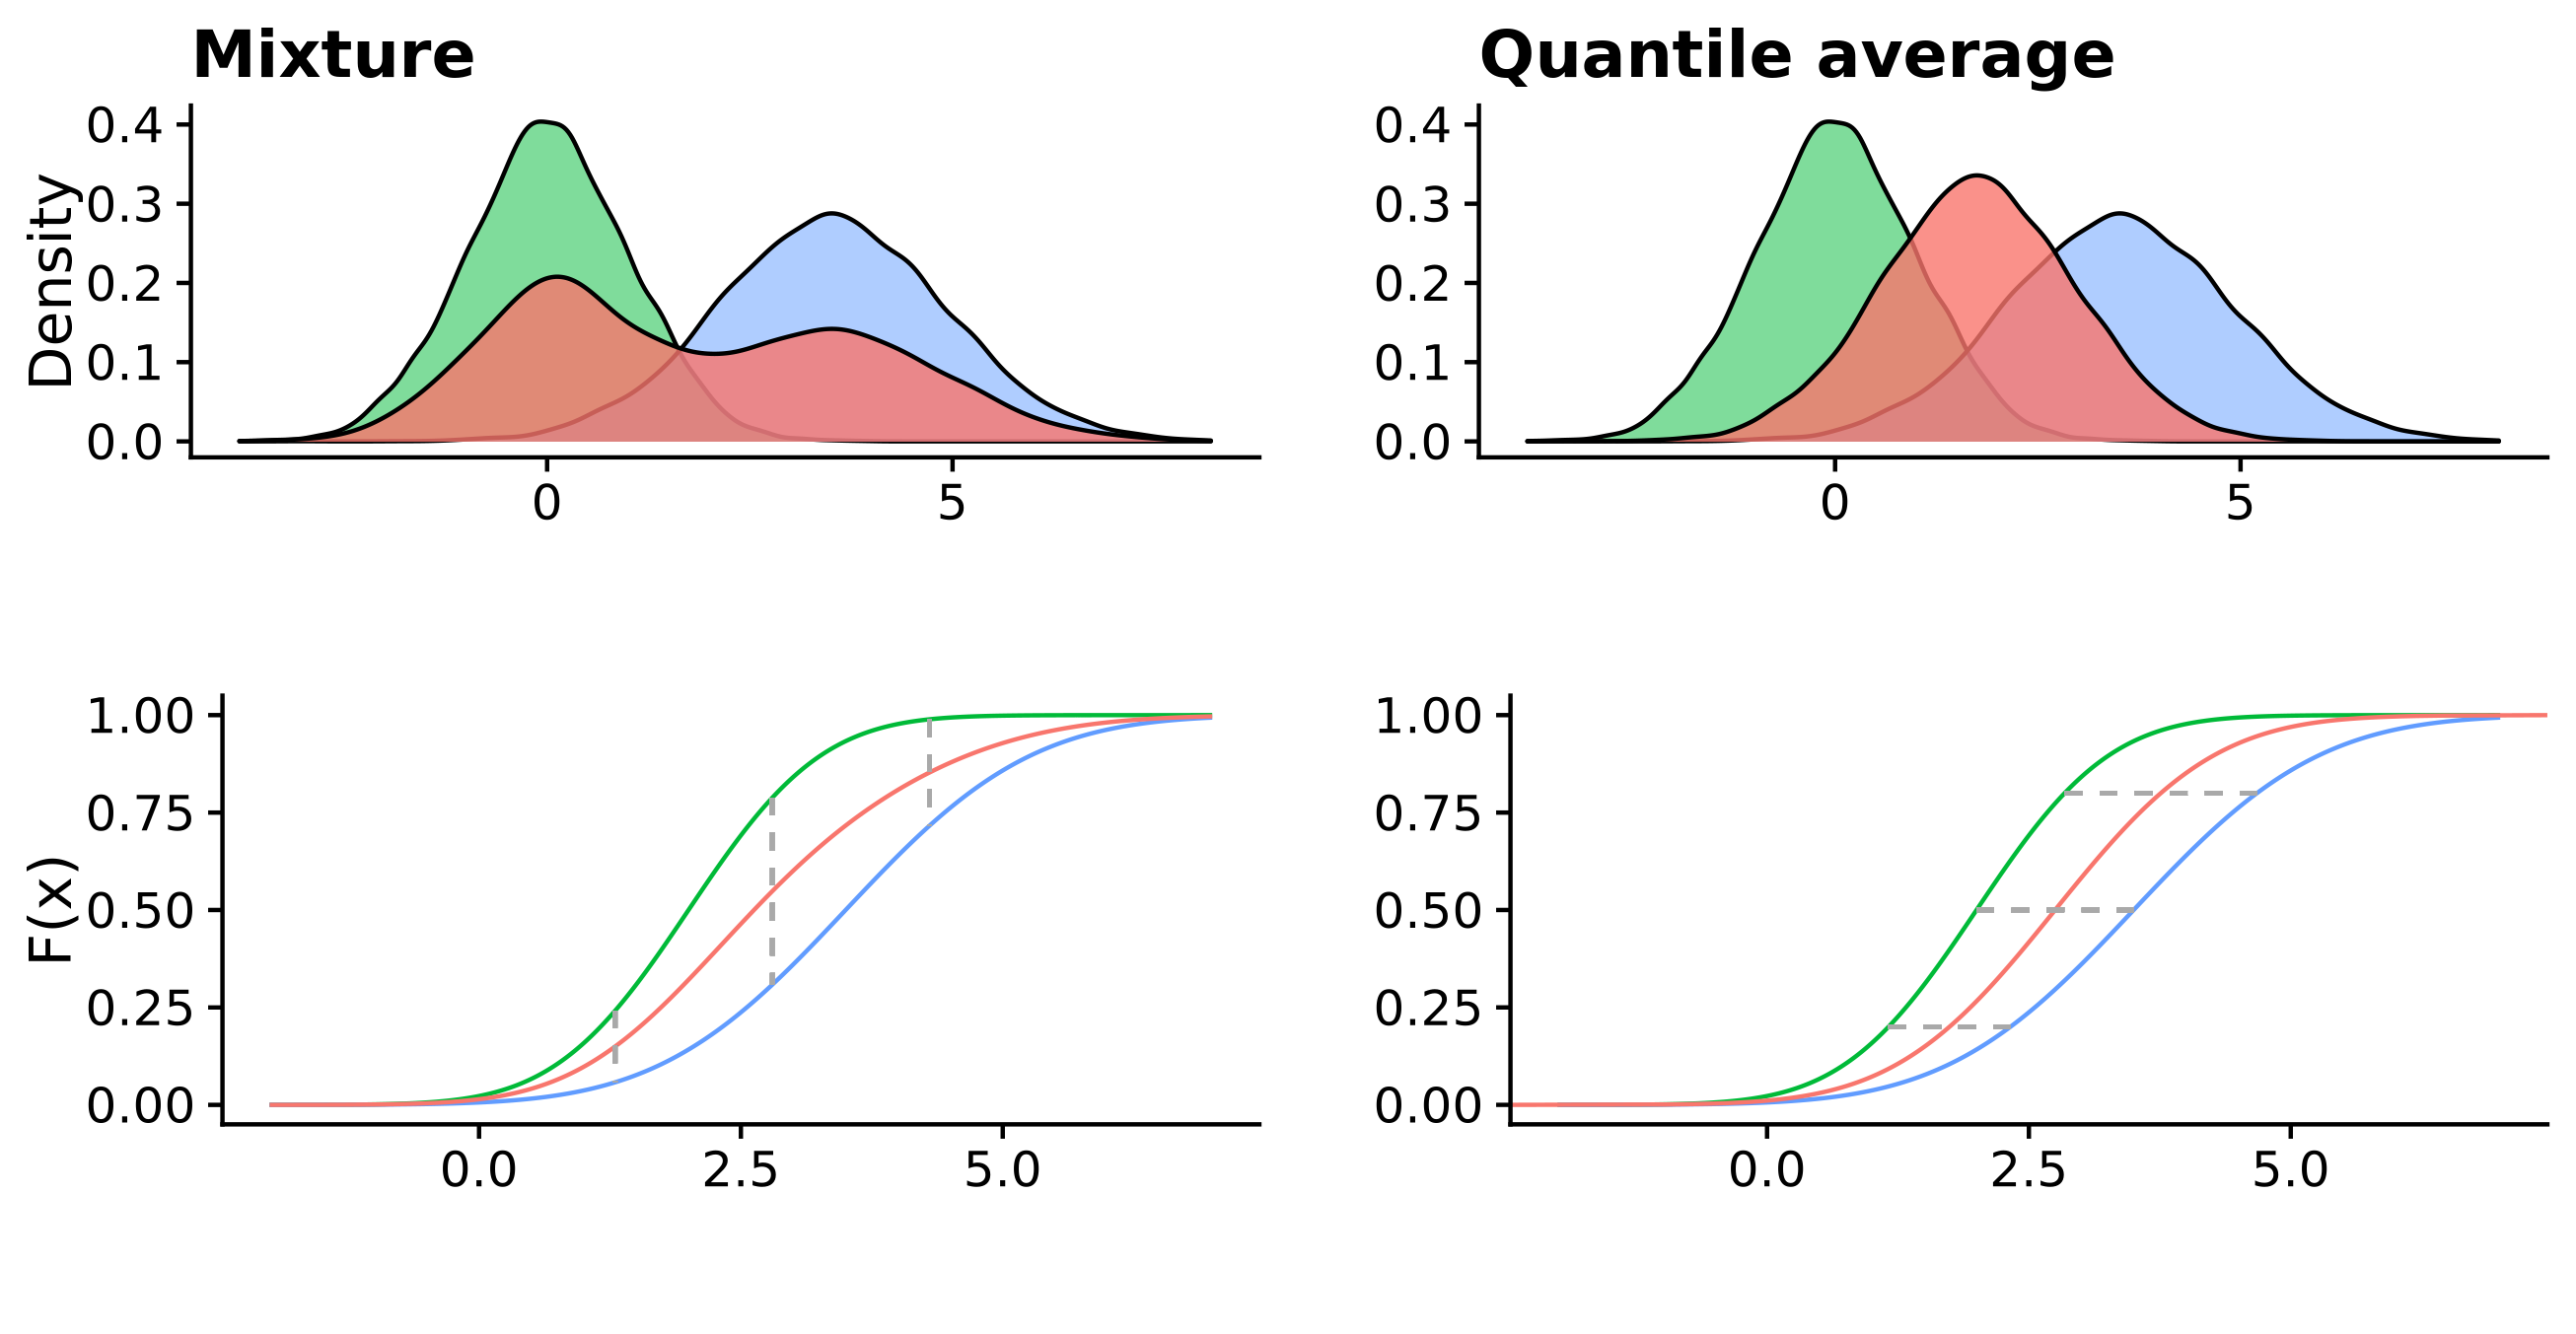
\includegraphics[width=0.95\linewidth]{../visualisation/chapter-4-ensemble/average-mixture-example} \caption{Two different ways of combining two predictive distributions (based on predictive samples). The left is a mixture distribution (red) generated by taking random samples with equal probability from the two original distributions (green and blue). The right is a quantile average that was generated by taking the pairwise mean of the sorted vectors of the predictive samples from the two distributions. The lower two plots show the same combinations in terms of averages of the cumulative distribution functions.}\label{fig:average-mixture-example}
\end{figure}

In the following, two different ensemble formation strategies will be presented. The Quantile Regression Average (QRA) is an ensemble strategy suited for quantile forecasts that determines optimal weights for a weighted quantile average. The CRPS ensemble works with predictive samples and determines optimal weights for a mixture distribution.

\hypertarget{the-quantile-regression-average-ensemble}{%
\section{The Quantile Regression Average ensemble}\label{the-quantile-regression-average-ensemble}}

The Quantile Regression Average \citep{nowotarskiComputingElectricitySpot2015} is an ensemble strategy build upon the weighted interval score presented in Chapter \ref{evaluation}.
Consider a forecast made for observation \(i, i = 1, \dots, n\) by one model \(k, k = 1, \dots, K\) at different quantile levels \(t \in (0,1), t=1,\dots, T\). The corresponding quantile prediction for observation i from model k at quantile level t is denoted \(q_{itk}\). The ensemble prediction at quantile level \(t\), \(q_{i, \text{ensemble},t}\) is then a weighted average of the corresponding predictive quantiles of the individual models:

\[q_{i,\text{ensemble}, t} = \sum_{k = 1}^K w_k \cdot q_{ikt}\],

where \(w_k\) is the weight given to model \(k\). The weights are usually constrained to be non-negative and to sum up to one. To get an optimal ensemble, we are looking for the combination of weights that, across all quantile levels \(t, t = 1, \dots, T\), produce an ensemble which minimises the weighted interval score over past observations. The optimisation problem can be denoted as follows \citep{ryantibshiraniQuantileStacking2020}:

\[\mathop{\text{arg min}}_{w} \sum_{i=1}^n \sum_{t=1}^T \psi_{_t} \bigg(y_i - \sum_{k=1}^K w_k q_{itk} \bigg) \]

where \(\psi_{t}()\) denotes the so-called pinball loss at quantile level \(t\). The pinball loss is defined as

\[\psi_{t}(x) = \max(t \cdot x, (t-1)\cdot x)\].

The solution to this minimisation problem yields the ensemble that minimises past weighted interval scores. This optimisation problem can be extended in a number of ways. E.g. one can estimate different weights for different quantile levels or one can incorporate additional constraints, e.g.~that quantiles not cross. The minimisation problem (including the additional constraints) can conveniently be solved using the quantgen package \citep{R-quantgen}.

\hypertarget{the-crps-ensemble}{%
\section{The CRPS ensemble}\label{the-crps-ensemble}}

Instead of the weighted interval score, we can also use the CRPS as a basis for an ensemble formation approach. The major conceptual advantage of using CRPS and predictive samples is that we can create a mixture distribution instead of a quantile average. The approach described in the following is a form of stacking (see \citet{yaoUsingStackingAverage2018}). Stacking is, in theory, optimal even if the true data-generating distribution is not among the individual ensemble distributions. While many other strategies like Bayesian Model Averaging eventually \citep{rafteryBayesianModelAveraging1997, hoetingBayesianModelAveraging1999, rafteryUsingBayesianModel2005} converge to putting all their weights to the single model that is closest to the true data-generating distribution, stacking is able to combine information from all models to form an optimal ensemble.

This CRPS ensembling approach was developed in collaboration with Yuling Yao from the Columbia University in New York and is implemented in the R package \texttt{stackr} \citep{R-stackr}. The following method overview is based on work written by Yuling Yao and edited by me for the \texttt{stackr} vignette.

As stated in Equation \eqref{eq:crps} in Chapter \ref{evaluation}, the CRPS for a predictive distribution with finite first moment and the corresponding true value \(y\) is given by
\[crps(F,y)=\mathbb{E}_X|X-y|- \frac{1}{2}\mathbb{E}_{X,X^\prime}|X-X'|\]
The notation now is slightly altered compared to Chapter \ref{evaluation} to avoid ambiguities with different versions of \(x\). The predictive distribution is denoted by \(F\) and true observed values are donated by \(y\). Let us assume we have data from \(T\) time points \(t = 1, \dots, T\) in \(R\) regions \(r = 1, \dots, R\). Observations are denoted \(y_{tr}\). Predictive samples are generated from \(K\) different models \(k = 1, \dots, K\). For every observation \(y_{tr}\) the \(S\) predictive samples \(s = 1, \dots, S\) are denoted \(x_{1ktr}, \dots, x_{Sktr}\).

Let us first look at the CRPS for one observation and one predictive model before deriving the CRPS of a mixture of all models. Based on the predictive samples, we can compute the CRPS of the \(k\)-th model for the observation \(y_{tr}\) at time \(t\) in region \(r\) as

\begin{align*}
 \widehat {\text{crps}}_{ktr} &= \widehat {\text{crps}}(x_{1ktr}, \dots, x_{Sktr},y_{tr}) \\
 &= \frac{1}{S} \sum_{s=1}^S  |x_{sktr}-y_{tr}| - \frac{1}{2S^2} \sum_{s, j=1}^S |x_{sktr}- x_{jktr}|
\end{align*}

Now we want to aggregate predictions from these \(K\) models. When the prediction is a mixture of the \(K\)
models with weights \(w_1, \dots, w_s\), the CRPS can be expressed as

\begin{align*}
 \widehat {\text{crps}}_{\text{ensemble}, tr} (w_1, \dots, w_K) 
 =& \frac{1}{S} \sum_{k=1}^K w_k  \sum_{s=1}^S |x_{skt}-y_t| \\
 &- \frac{1}{2S^2}  (\sum_{k=1}^K   \sum_{k, k'=1 }^K w_k w_{k'}   \sum_{s, j=1}^S |x_{skt}- x_{jk't}| )
\end{align*}

The overall CRPS for the mixture of all models for all observations can then simply be obtained by summing up the individual CRPS contributions from the different pairs of observations and predictions over all regions and time points. We can extend this framework by assigning different weights to different time points and regions. This makes sense for example if we want to assign less weight to older observations because we believe they are less characteristic of the current and future dynamics. Similarly, we might want to give more or less weight to certain regions. Mathematically we can introduce a time-varying weight \(\lambda_1, \dots, \lambda_T\), e.g.~\(\lambda_t = 2-(1-t/T)^2\) to penalize earlier estimates. Likewise we can introduce a region-specific weight \(\tau_r\).

To obtain the optimal CRPS weights we finally solve a quadratic optimisation:

\begin{align*}
 &\min_{w_1, \dots, w_K} \sum_{t=1}^T  \sum_{r=1}^R\lambda_t\tau_r  \widehat {crps}_{\text{ensemble}, tr} (w), \\
  &s.t. ~{0\leq w_1, \dots, w_K \leq 1, \sum_{k=1}^K w_k=1}. 
\end{align*}

In \texttt{stackr}, this is implemented using the \texttt{optimizing} function from the \texttt{rstan} \citep{R-rstan} package. To speed up computation, the terms \(\sum_{s=1}^S |x_{skt}-y_{tr}|\), \(\sum_{s, j=1}^S |x_{sktr}- x_{jktr}|\), and \(\sum_{s, j=1}^S |x_{sktr}- x_{jk'tr}|\) are only computed once for all \(k, k'\) pairs. Currently, \texttt{stackr} does not yet support different forecast horizons, but instead one horizon has to be chosen to optimise for.

After having obtained the mixture weights we can now obtain the final mixture by drawing samples from the individual member distribution distributions with probability equal to the weight asssigned to the corresponding model. This is implemented in the function \texttt{mixture\_from\_samples} in \texttt{stackr}. The following code snippet illustrates how a CRPS ensemble can be obtained using \texttt{stackr}:

\(~\)

\begin{Shaded}
\begin{Highlighting}[]
\NormalTok{splitdate \textless{}{-}}\StringTok{ }\KeywordTok{as.Date}\NormalTok{(}\StringTok{"2020{-}03{-}28"}\NormalTok{)}
\NormalTok{data \textless{}{-}}\StringTok{ }\NormalTok{data.table}\OperatorTok{::}\KeywordTok{setDT}\NormalTok{(stackr}\OperatorTok{::}\NormalTok{example\_data)}
\KeywordTok{print}\NormalTok{(data, }\DecValTok{3}\NormalTok{, }\DecValTok{3}\NormalTok{)}
\end{Highlighting}
\end{Shaded}

\begin{verbatim}
##         geography model sample_nr       date   y_pred    y_obs
##      1:  Tatooine ARIMA         1 2020-03-14 1.719445 1.655068
##      2:  Tatooine ARIMA         2 2020-03-14 1.896555 1.655068
##      3:  Tatooine ARIMA         3 2020-03-14 1.766821 1.655068
##     ---                                                       
## 103998: Coruscant Naive       498 2020-04-08 1.433936 1.543976
## 103999: Coruscant Naive       499 2020-04-08 1.719357 1.543976
## 104000: Coruscant Naive       500 2020-04-08 0.781818 1.543976
\end{verbatim}

\begin{Shaded}
\begin{Highlighting}[]
\NormalTok{traindata \textless{}{-}}\StringTok{ }\NormalTok{data[date }\OperatorTok{\textless{}=}\StringTok{ }\NormalTok{splitdate]}
\NormalTok{testdata \textless{}{-}}\StringTok{ }\NormalTok{data[date }\OperatorTok{\textgreater{}}\StringTok{ }\NormalTok{splitdate]}

\CommentTok{\# Obtain weights based on training data}
\NormalTok{weights \textless{}{-}}\StringTok{ }\NormalTok{stackr}\OperatorTok{::}\KeywordTok{crps\_weights}\NormalTok{(traindata)}

\CommentTok{\# create mixture based on predictive samples in the testing data. }
\NormalTok{test\_mixture \textless{}{-}}\StringTok{ }\NormalTok{stackr}\OperatorTok{::}\KeywordTok{mixture\_from\_samples}\NormalTok{(testdata, }\DataTypeTok{weights =}\NormalTok{ weights)}
\KeywordTok{print}\NormalTok{(test\_mixture)}
\end{Highlighting}
\end{Shaded}

\begin{verbatim}
##        geography       date    y_pred sample_nr        model
##     1:  Tatooine 2020-03-29 0.7475794         1 crps_mixture
##     2:  Tatooine 2020-03-29 0.6369094         2 crps_mixture
##     3:  Tatooine 2020-03-29 1.5239227         3 crps_mixture
##     4:  Tatooine 2020-03-29 1.3241245         4 crps_mixture
##     5:  Tatooine 2020-03-29 0.9995749         5 crps_mixture
##    ---                                                      
## 10996: Coruscant 2020-04-08 0.4987309       496 crps_mixture
## 10997: Coruscant 2020-04-08 0.0000000       497 crps_mixture
## 10998: Coruscant 2020-04-08 2.1036704       498 crps_mixture
## 10999: Coruscant 2020-04-08 0.3992655       499 crps_mixture
## 11000: Coruscant 2020-04-08 0.2112317       500 crps_mixture
\end{verbatim}

\hypertarget{background-data}{%
\chapter{Data and forecasting models}\label{background-data}}

After Chapters \ref{evaluation} and \ref{model-aggregation} have described the theoretical foundations of model evaluation and model aggregation, this chapter gives a first overview of the data and the different forecasting models analysed in Chapter \ref{results} to provide some context for the ensuing evaluation. It first describes the Forecasting Hub in more detail and offers a first look at the data. It then gives a brief overview of the different forecasting models.

\hypertarget{introduction-to-the-covid-19-forecast-hub-and-overview-of-the-data}{%
\section{Introduction to the COVID-19 Forecast Hub and overview of the data}\label{introduction-to-the-covid-19-forecast-hub-and-overview-of-the-data}}

The COVID-19 Forecast Hub \citep{umass-amherstinfluenzaforecastingcenterofexcellenceCovid19forecasthubOrg2020} is a collaboration between the U.S. Centers for Disease Control and Prevention (CDC), academic research groups led by Professor Nicholas Reich at the University of Massachussets Amherst, and different industry partners. Starting on April 13, the consortium elicited weekly forecasts for all US states and territories and the US as a whole from research teams around the world. Forecasts were submitted every Monday in a probabilistic format. The predictive distribution was represented by the median and eleven prediction intervals ranging from a 10\% prediction interval to a 98\% prediction interval (i.e.~the following 23 quantiles were recorded: \texttt{c(0.01,\ 0.025,\ seq(0.05,\ 0.95,\ by\ =\ 0.05),\ 0.975,\ 0.99)}). Forecasts were made for one to (at least) four week ahead horizons of targets like daily or weekly deaths and case numbers.

Out of these targets, this we focus only on weekly death incidences. The forecasts we analysed were made between June 22nd 2020 and August 3rd 2020 in twelve different US states and the US as a whole. As the ensemble models need at least one week of past data to estimate weights, only forecasts between June 29th and August 3rd. were evaluated. Eight models were chosen from all Forecast Hub models in a way that attempts to reflect the variety of models submitted to the Hub. Among these models also was the `epiforecasts-ensemble1' model that was submitted by the working group at the London School of Hygiene and Tropical Medicine that co-supervised this work. Dates and locations were chosen to obtain a complete set of predictions with no missing forecasts for any location or time point. While this isn't strictly necessary, it avoids downstream complications with model aggregation and evaluation that are beyond the scope of this thesis.

The ground truth data is provided by the Center for Systems Science and Engineering (CSSE) at Johns Hopkins University \citep{dongInteractiveWebbasedDashboard2020}. Table \ref{tab:overview} gives an overview of the dates, locations and models included. Figure \ref{fig:us-data} shows observed deaths in all thirteen locations. The time frame that is actually analysed is highlighted in green. We can see that the evolution of deaths exhibits quite different dynamics across different locations. In states like Illinois, Maryland or Massachusetts, deaths were mostly constant or falling. In others, like Arizona, Florida or Texas, deaths showed a strong upwards trend. Chapter \ref{results} will analyse in detail how models fare in these different scenarios.

\begin{figure}
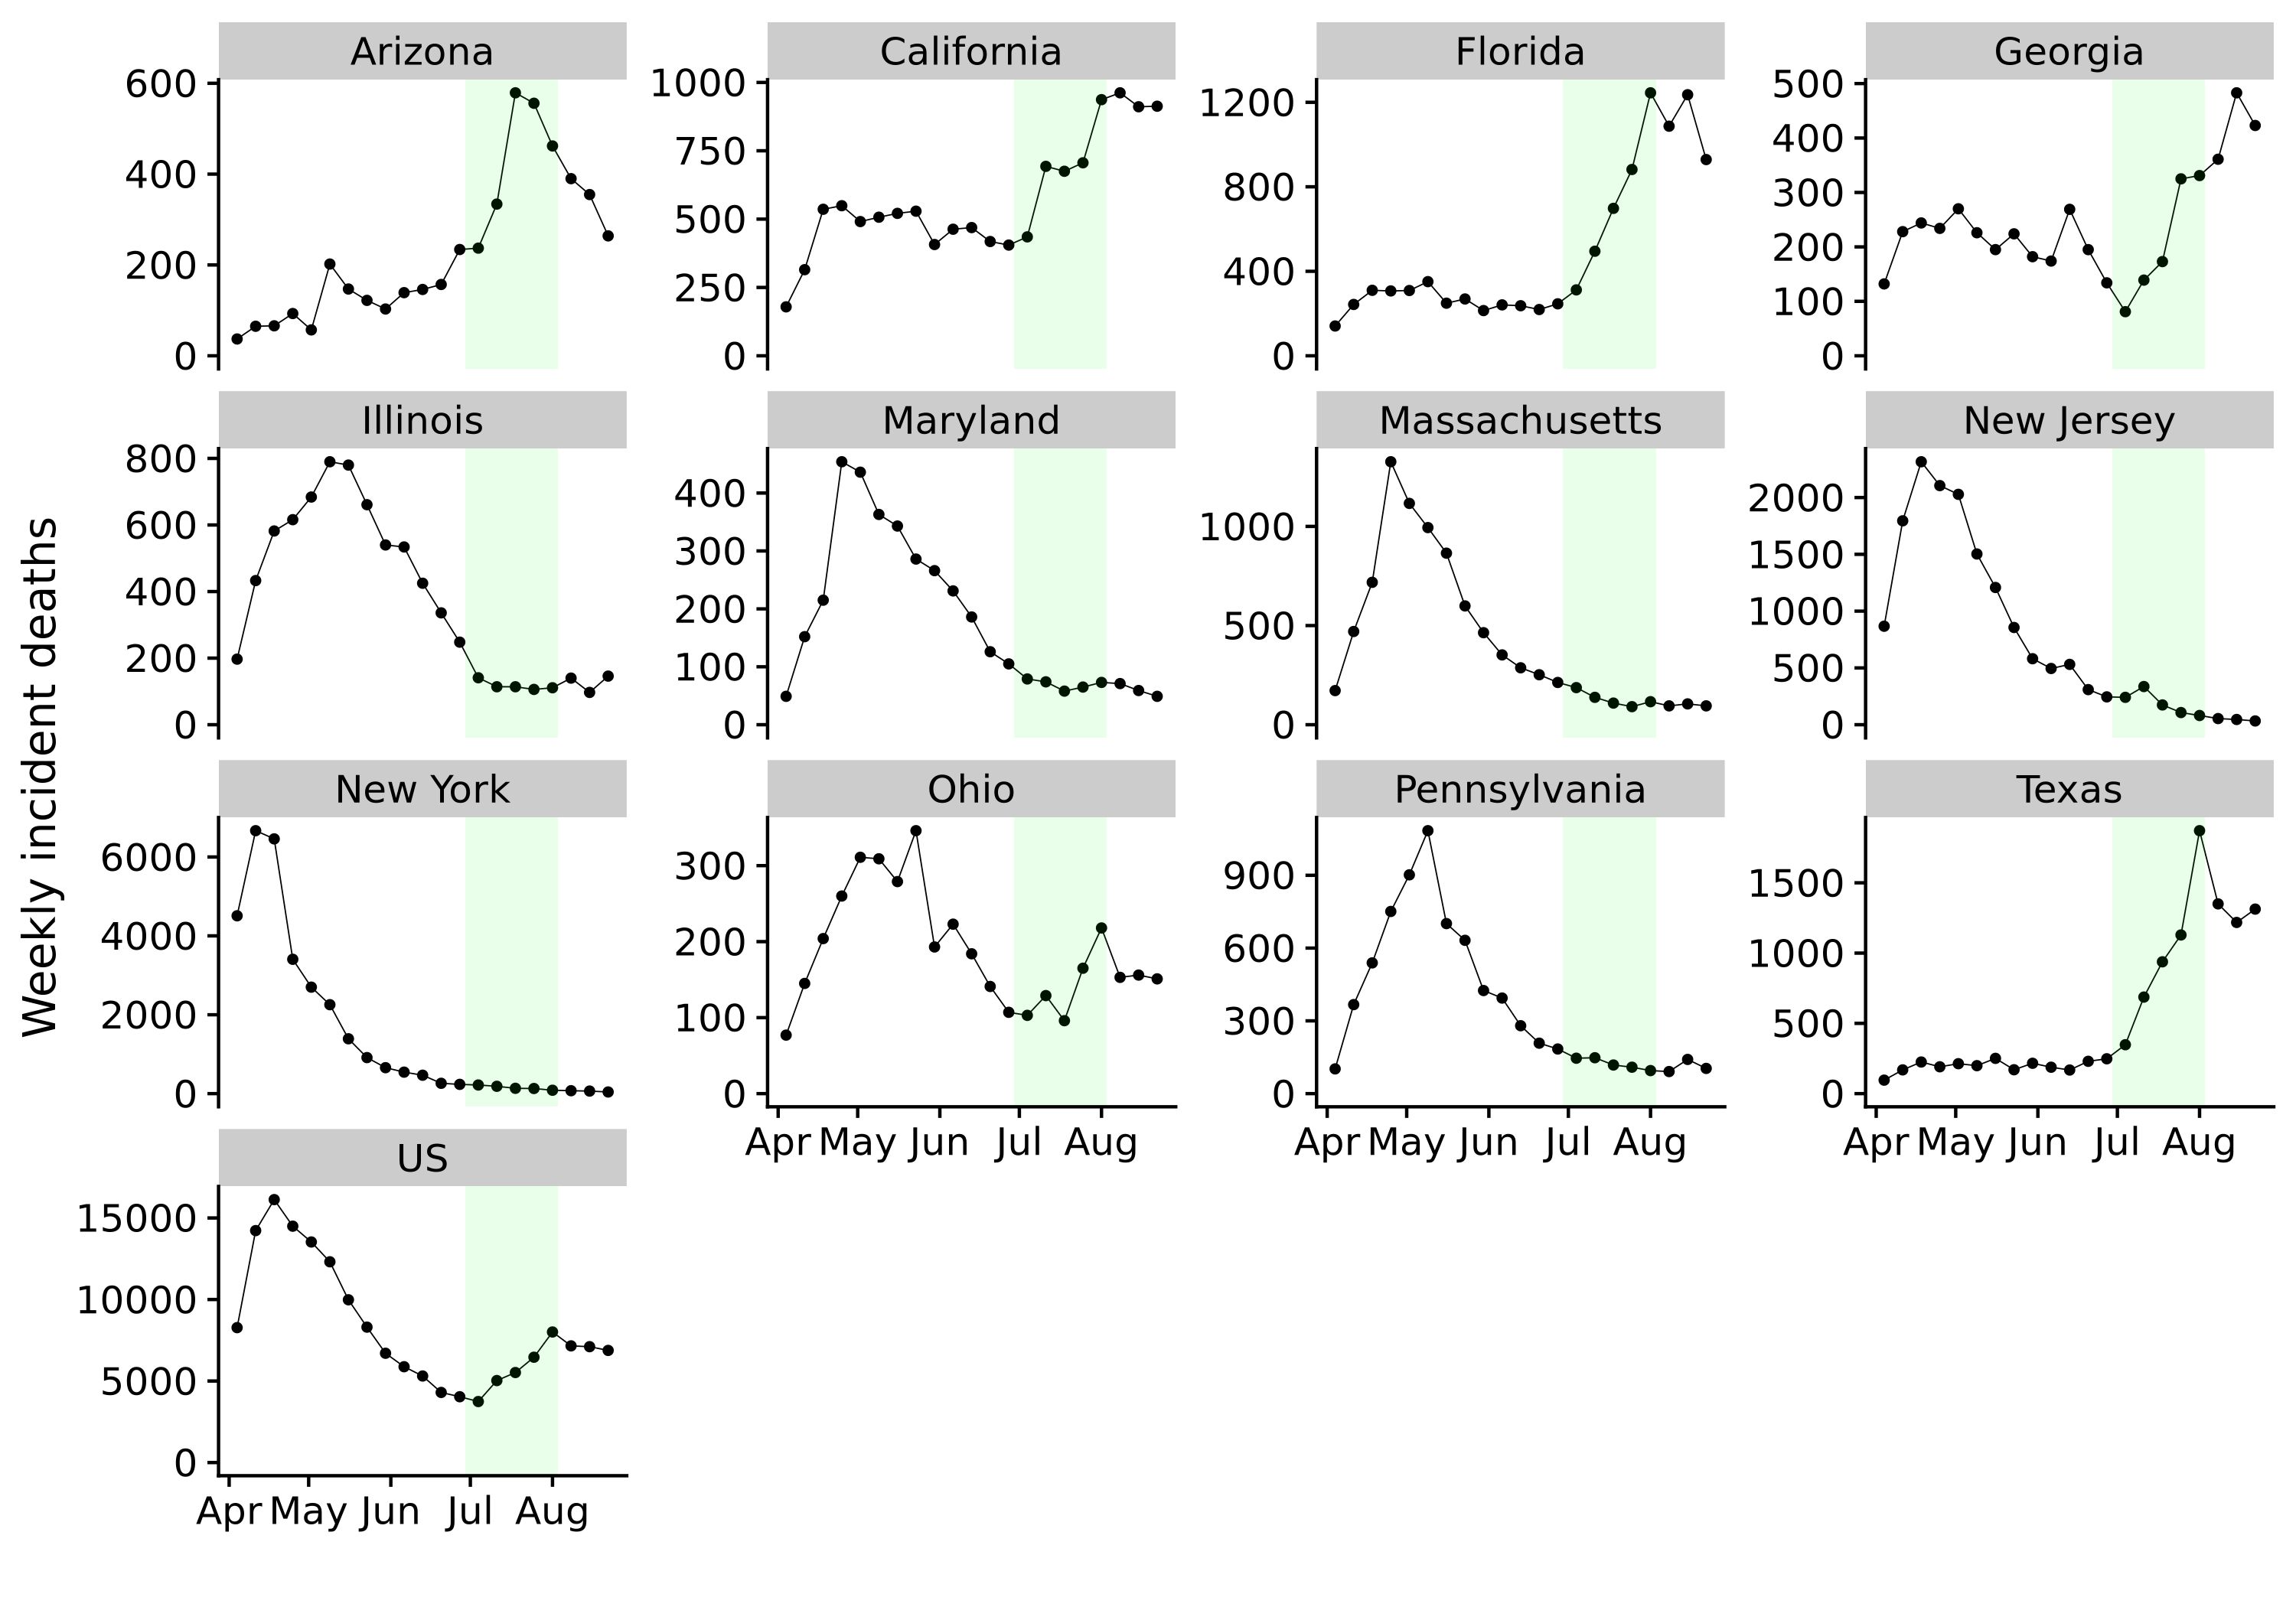
\includegraphics[width=0.95\linewidth]{../visualisation/chapter-2-background-data/plot-observations} \caption{Observed deaths in different regions. Weeks for which predictions are analysed are highlighted in green.}\label{fig:us-data}
\end{figure}

\hypertarget{an-overview-the-different-forecast-models}{%
\section{An overview the different forecast models}\label{an-overview-the-different-forecast-models}}

The models analysed in-depth in the next chapter vary substantially in the way they generate predictions. This section therefore gives a quick overview of the different model types. This overview should not be thought of as an exhaustive discussion, but is merely intended as a short primer that allows us to mentally place the COVID-19 Forecast Hub models in broad categories. The information used to inform this overview is taken from the descriptions provided by the research teams themselves\footnote{Model descriptions were uploaded by the teams on \href{https://github.com/reichlab/covid19-forecast-hub/tree/master/data-processed}{github.com/reichlab/covid19-forecast-hub/tree/master/data-processed}. The descriptions were accessed on 07.08.2020. As descriptions on github are updated whenever the model changes, this overview may therefore not be entirely accurate for all models over the entire history of past submissions included in the analysis.}.

Among the most widely used models in epidemiology are so-called compartmental models (see e.g.~\citet{brauerCompartmentalModelsEpidemiology2008} for an extensive overview). These split the general population in compartments and model the flow between these compartments. The basic compartments are \emph{Susceptible} (S), \emph{Infectious} (I) and \emph{Recovered} (R), giving these models the name SIR models. The flow from one compartment to the other is usually modeled using a set of differential equations. Compartmental models help to model specific characterisitcs of people in different compartments. For example, People in the \emph{Susceptible} compartment can be infected, while those who are in the \emph{Recovered} compartment are assumed to be immune against further infection. Compartmental models are therefore able to model the depletion of susceptibles as the epidemic progresses. Other compartments, like \emph{Exposed but not infectious} (E) can be introduced ad libitum to model e.g.~incubation periods. Most models submitted to the Forecast Hub are compartmental models. Three models analysed here belong to that category: UMass-MechBayes, YYG-ParamSearch and CU-select.

UMass-MechBayes\footnote{\href{https://github.com/dsheldon/covid}{github.com/dsheldon/covid}} is a Bayesian model build from a classical SEIR compartmental model. The model is fit independently to each state and allows its parameters to vary over time.

The YYGParamSearch model\footnote{\href{https://covid19-projections.com}{covid19-projections.com} and \href{https://github.com/youyanggu/covid19_projections}{github.com/youyanggu/covid19\_projections}} adds an additional machine learning layer to a classical SEIR model to learn optimal hyperparameters for the model. Some of the parameters like the infectious period are shared across locations, but most parameters like the mortality from Covid-19 or the effetive reproduction number \(R_t\) (the average number of people each infected person will infect in turn, see e.g.~\citet{nishiuraEffectiveReproductionNumber2009} or \citet{coriNewFrameworkSoftware2013}) etc. are determined per state.
The CU-select model is a SEIR model that is augmented by human insight. The Columbia University regularly submits a range of projections under different scenarios. For the CU-select model they always hand-pick the one they believe is most plausible.

Another common approach is to model the evolution of the pandemic using a time-varying growth rate. Based on the assumption that the spread of a disease is exponential in nature it is intuitive to estimate future case numbers by modeling the growth rate. The LANL-GrowthRate model and to a certain extent the epiforecasts-ensemble1 take this approach.

The LANL-GrowthRate model is a two component model. The first component models the number of infections using a time-varying growth parameter that connects present (or future) infections to earlier infections and the number of susceptibles. In a second step, this infections get mapped to reported deaths by assuming a fraction of infections likely to die.

The epiforecasts-ensemble combines the growth rate approach with classical time series modeling. It consists of three submodels that were aggregated using first an equally weighted quantile average and later a quantile regression average. The three submodels were two time series models and an \(R_t\)-based prediction model. \(R_t\) denotes the effective reproduction number, i.e.~the average number of people each infected person will infect. The two timeseries models were generated using the forecastHybrid package \citep{R-forecastHybrid}. The package automatically selects an Autoregressive Integrated Moving Average (ARIMA) model or a State Space model with appropriate error, trend and seasonality (ETS model). One of the epiforecasts-ensemble1 timeseries models included current cases as a lagged predictor, while the other was based on deaths only. The third model was generated using the R packages \texttt{EpiSoon} \citep{R-EpiSoon}, \texttt{EpiNow} \citep{R-EpiNow}, and later \texttt{EpiNow2} \citep{R-EpiNow2}. \texttt{EpiSoon} takes in reported cases to estimate the trajectory of \(R_t\). This trajectory is then forecasted into the future using \texttt{forecastHybrid} and transformed back to incidences using the so-called renewal equation that models futures cases as a weighted sum of past cases times \(R_t\). These three models are fit independently to each location.

A third possibility is to model deaths more directly in terms of a regression framework. This the approach chosen by the UT-Mobliity model \citep{woodyProjectionsFirstwaveCOVID192020}) that employs a Bayesian negative binomial regression model. One of the major predictors used is GPS mobility data provided by a company called SafeGraph. This data is used to compute measures of social distancing that are ultimately fed into the regression model.

In order to provide a sensible baseline to compare models against, the Forecast Hub created the COVIDhub-baseline model. This model basically assumes that incidences will be the same as in the past and models the uncertainty around this estimate according to the distribution of past changes in incidences. More precisely, forecasts for incidences are generated in the following way: The timeseries of all past incidences is taken and first differences are formed. These first differences, as well as the negative of these incidences are then used further along. From this vector of past changes, samples are drawn to get a predictive distribution of future changes. A predictive distribution for future incidences is then obtained by adding these samples to the last observed incidence. The predictive distribution is then shifted to enforce that the mean of the distribution equals the last observed value. Incidences below zero are truncated, and quantiles are obtained from the samples.
In addition to the models described above, four model ensembles were analysed. One of these ensembles, the COVIDhub-ensemble was an ensemble created by the Forecast Hub itself using a quantile average approach. The model was formed by taking the arithmetic mean of the corresponding quantiles from all eligible models. Models are deemed eligible if they pass some general sense checks (e.g.~cumulative forecasts must in general not decrease over time). The number of models included varies from state to state as not all teams submit forecasts for all locations. The other three ensembles were formed from the above described eight original models.

The mean-ensemble is a simple equally weighted quantile average of all original models. All models included in the mean-ensemble are therefore also included in the COVIDhub-ensemble. We can therefore think of the mean-ensemble as a variotion of the COVIDhub-ensemble that puts higher weight on the models included in this analysis and zero weight to the models excluded. The mean-ensemble serves as an important control. Any performance difference between the two ensembles can be attributed to the effect of the selection of models included for the analysis.

The qra-ensemble is formed based on the two last weeks of data using the methodology outlined in Chapter \ref{model-aggregation}. The qra-ensemble takes all past forecasts for which we have observations into account. It is therefore created using one and two-week-ahead forecasts. For the first evaluation date, June 29th, only one week of past data was used to inform the ensemble weights. Two weeks of past data were chosen as a sensible default, instead of optimised for, in order to avoid overfitting. Chapter \ref{results}, however, also provides a sensitivity analysis that explores other choices.

The crps-ensemble was also formed using two weeks of past data. But in order to make model aggregation possible, forecasts had to be transformed first. While the CRPS ensemble approach described in Chapter \ref{model-aggregation} is based on predictive samples, the Forecast Hub only stores predictive distributions in a quantile forecast. We therefore fit a separate gamma distribution to every set of predictive quantiles. The gamma distribution was chosen for its simplicity and reasonably good fit. The fitted distributions were subsequently used to obtain 1 000 predictive samples per forecast. We then estimated weights based on the predictive samples and created a mixture distribution by random sampling from the individual model samples with probability equal to the estimated weights. The samples drawn for the mixture model were then again used to create quantiles. This approach is not ideal as it is bound to lose information. Overall, however, it seemed to have worked not too badly. Figure \ref{fig:difference-true-sampled} shows the difference between quantiles from the actual predictive distributions submitted to the Forecast Hub and sample quantiles obtained by random sampling from a gamma distribution fitted to the same forecasts. This figure includes all forecasts for all locations, forecast dates and quantiles at once, so it may not show the full picture. It broadly suggests however, that the approach works reasonably for most quantiles of the predictive distribution. For higher quantiles we can see substantial deviations. As \texttt{stackr} currently does not support multiple forecast horizons, a choice also had to be made for a forecast horizon to optimise for. We chose to optimise for two-week-ahead forecasts. This effectively means that the crps-ensemble could use less data than the qra-ensemble, as forecasts from the previous week did not yet have matching observations and therefore only the two-week-ahead forecasts from two weeks ago could be used. Again, other possible choices for these parameters are explored in Chapter \ref{results}.

\begin{figure}
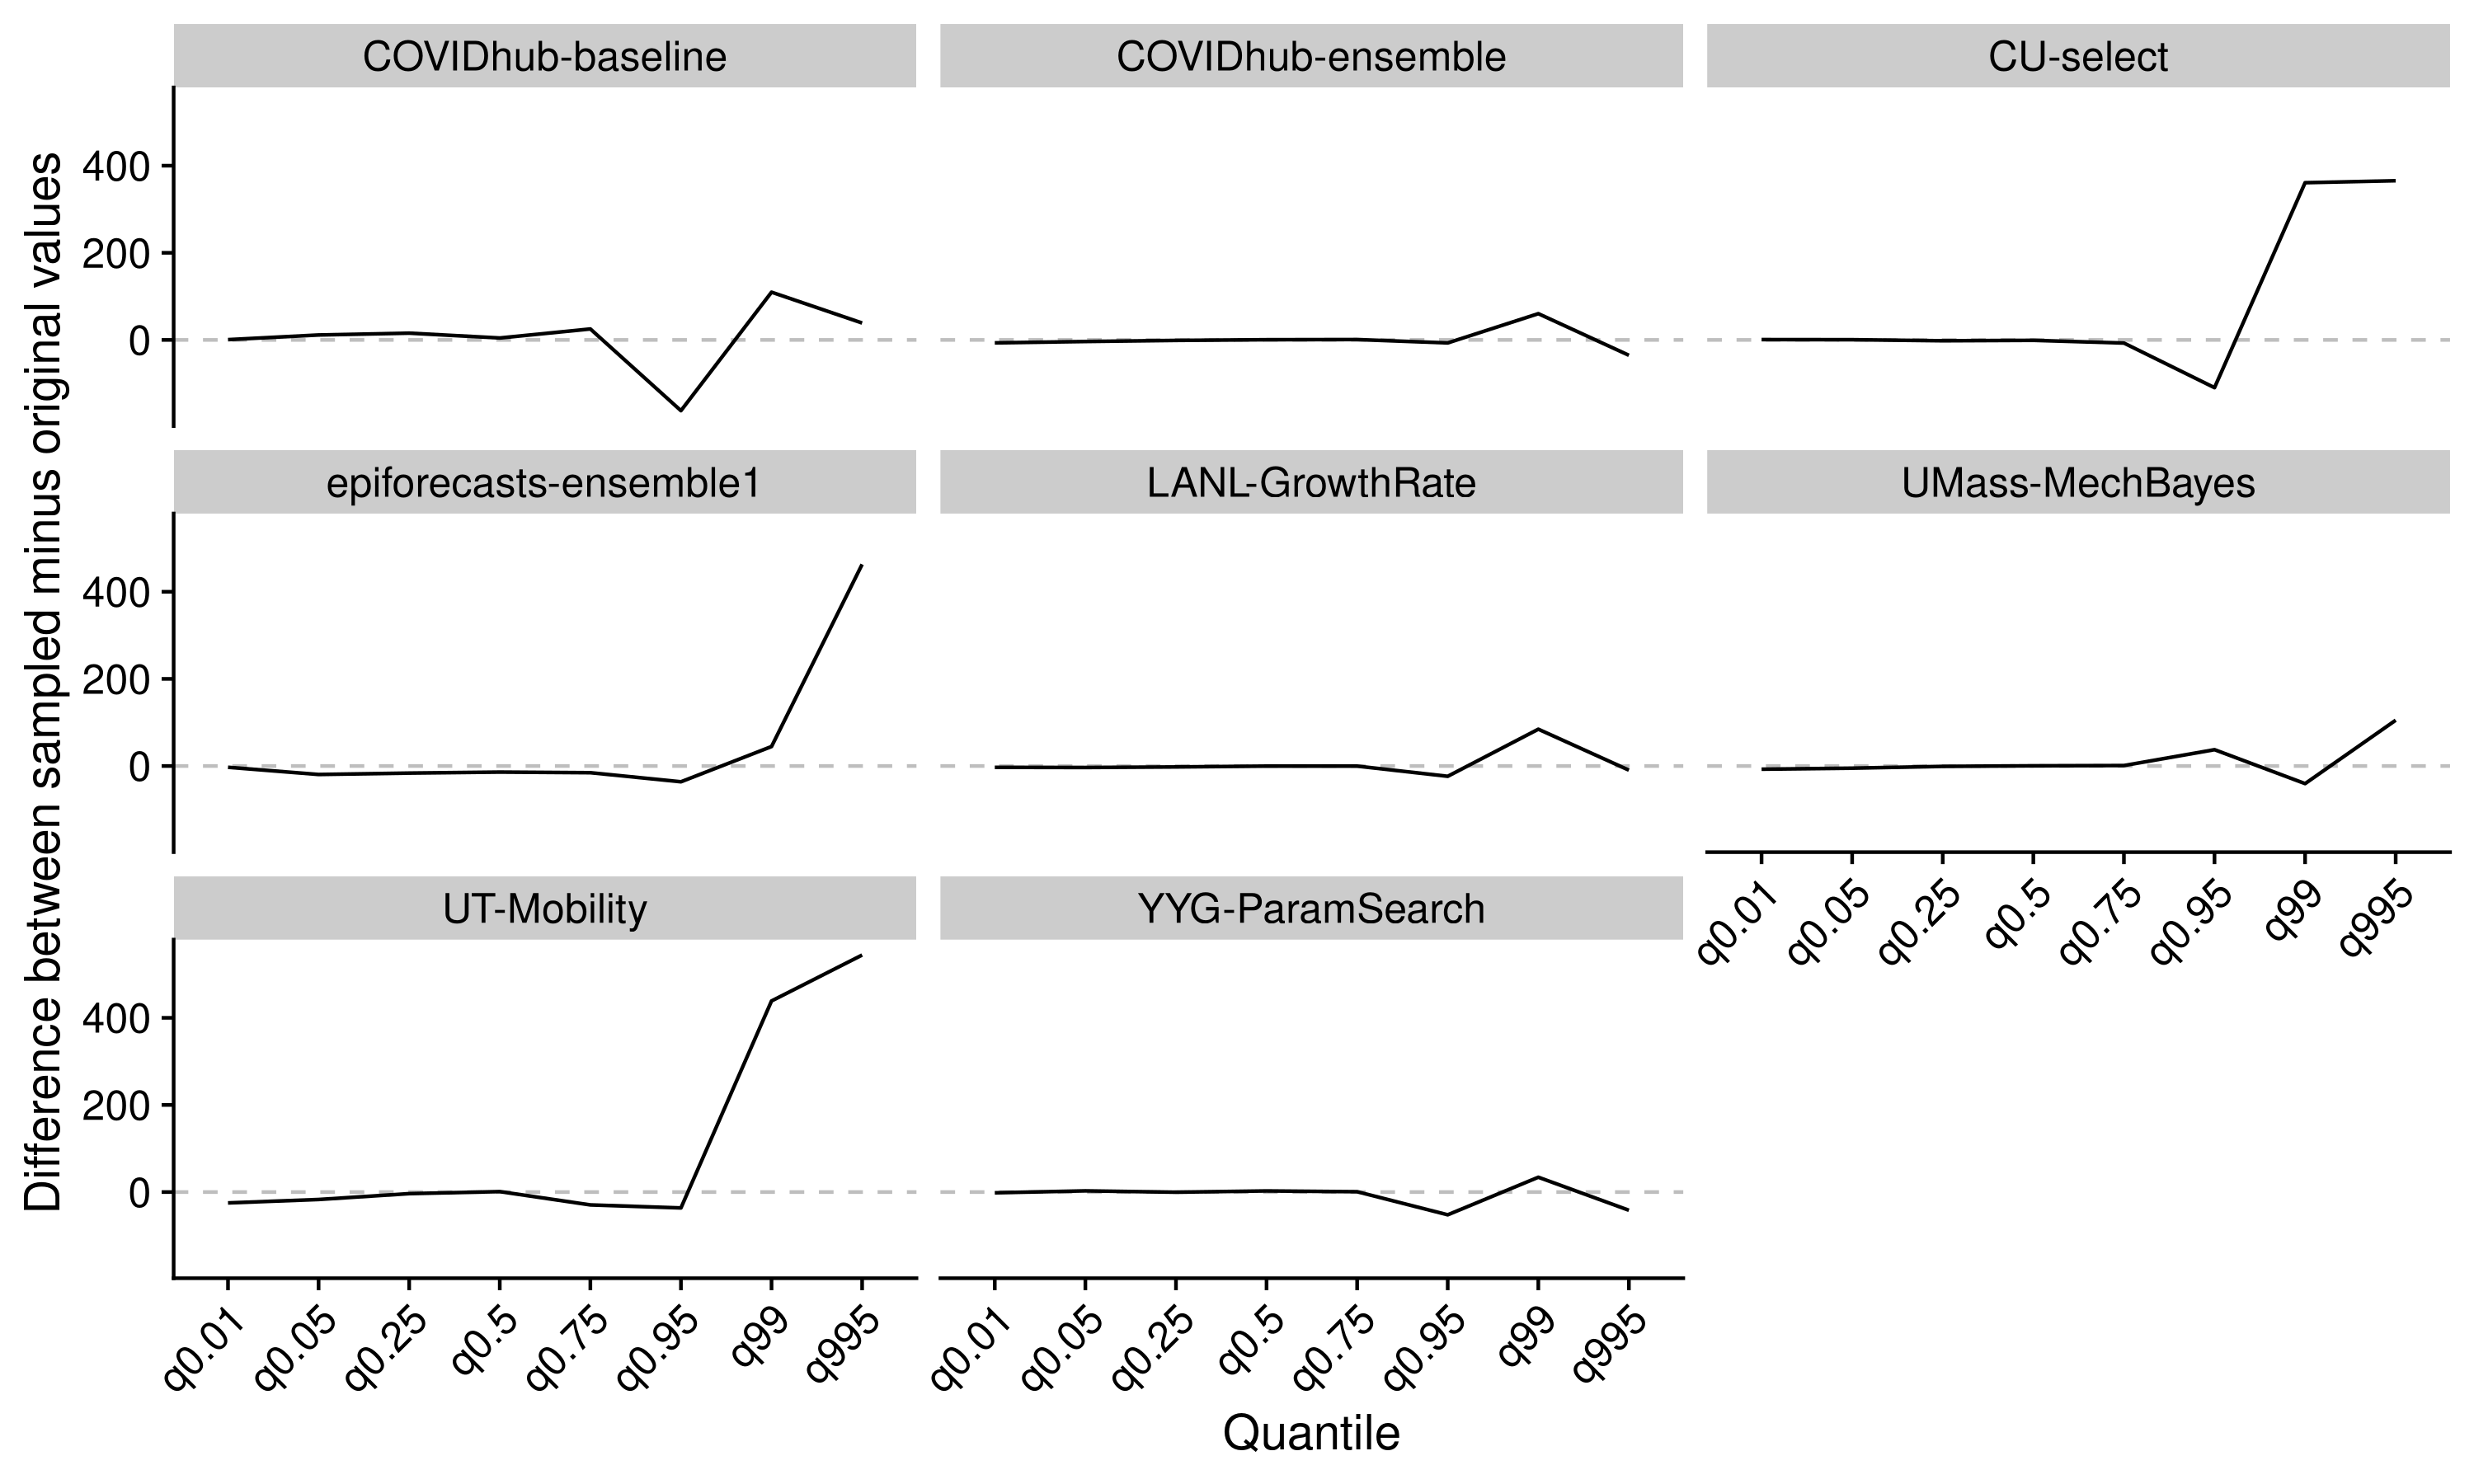
\includegraphics[width=0.95\linewidth]{../visualisation/chapter-4-ensemble/difference-true-sampled} \caption{Observed deaths in different regions. Weeks for which predictions are analysed are highlighted in green.}\label{fig:difference-true-sampled}
\end{figure}

Table \ref{tab:overview} provides a convenient summary of the different locations, forecast dates and models included in the analysis.

\label{tab:overview}An overview of the locations, dates and models included in the analysis.

locations

dates

models

model summary

Arizona

2020-06-29

COVIDhub-baseline

Baseline prediction model

California

2020-07-06

COVIDhub-ensemble

Official quantile average ensemble

Florida

2020-07-13

epiforecasts-ensemble1

time series / growth rate model

Georgia

2020-07-20

UMass-MechBayes

Bayesian SEIR model

Illinois

2020-07-27

YYG-ParamSearch

Machine Learning / SEIR model

Maryland

2020-08-03

CU-select

SEIR / human selection model

Massachusetts

UT-Mobility

Regression model

New Jersey

LANL-GrowthRate

Growth rate model

New York

Ohio

mean-ensemble

Quantile average ensemble

Pennsylvania

qra-ensemble

QRA ensemble

Texas

crps-ensemble

CRPS ensemble

US

\hypertarget{results}{%
\chapter{Results - evaluation and aggregation of Covid-19 death forecasts}\label{results}}

Chapters \ref{evaluation} and \ref{model-aggregation} have introduced the tools we need for model evaluation and model aggregation. Chapter \ref{results} will now apply these instruments to the Forecast Hub with the goal of better understanding their behaviour.

The majority of this chapter will deal with the evaluation of the eight models described in Chapter \ref{background-data} as well as the three different ensembles of the eight original models. This evaluation is as much about understanding model performance in the Forecast Hub as it is about understanding the tools used for evaluation themselves. The chapter will therefore digress at times to look at additional things like how different metrics correlate. A large part of model assessment is visual in nature - the chapter will therefore involve a lot of discussion of visual representations of different evaluation aspects. The evaluation will follow the general structure proposed in Chapter \ref{evaluation}: First the forecasts will be visually inspected. Afterwards, the attention will turn to the summarised scores and metrics, followed by a detailed look at calibration (including bias, coverage and PIT histograms) and sharpness. A mixed-effects model of the weighted interval score will help to summarise the conclusions from the model evaluation. WHERE TO PUT THE MIXED MODEL?

The evaluation is followed by a more detailed look at the ensemble models that will discuss some specific aspects in more detail. These include a look at ensemble weights over time as well as analysis of different ensemble alternatives. REPHRASE THIS.

The chapter will conclude with a brief sensitivity analysis that serves as a quick check of the plausibility of the inferences made throughout the chapter.

\hypertarget{forecast-visualisation}{%
\section{Forecast visualisation}\label{forecast-visualisation}}

In order to get a general sense for how the models do we shall start with a look at the projections versus the actual data. Figure \ref{fig:models-us} gives an overview of the projections for one and four week ahead forecasts for the United States as a whole. Plots for other locations can be seen in the APPENDIX. From a brief look we can see that most models generally do a good job at capturing the dynamic one week ahead into the future. For four-week-ahead predictions, performance seems to deteriorate significantly. The mean-ensemble, the crps-ensemble and the UMass-MechBayes model seem to do a consistently good job at one and four week ahead predictions. The UT-Mobility looks good for one week ahead (except for the last time point), but performs poorly four weeks ahead. The LANL-GrowthRate model seems rather off regardless of the horizon.

\begin{figure}
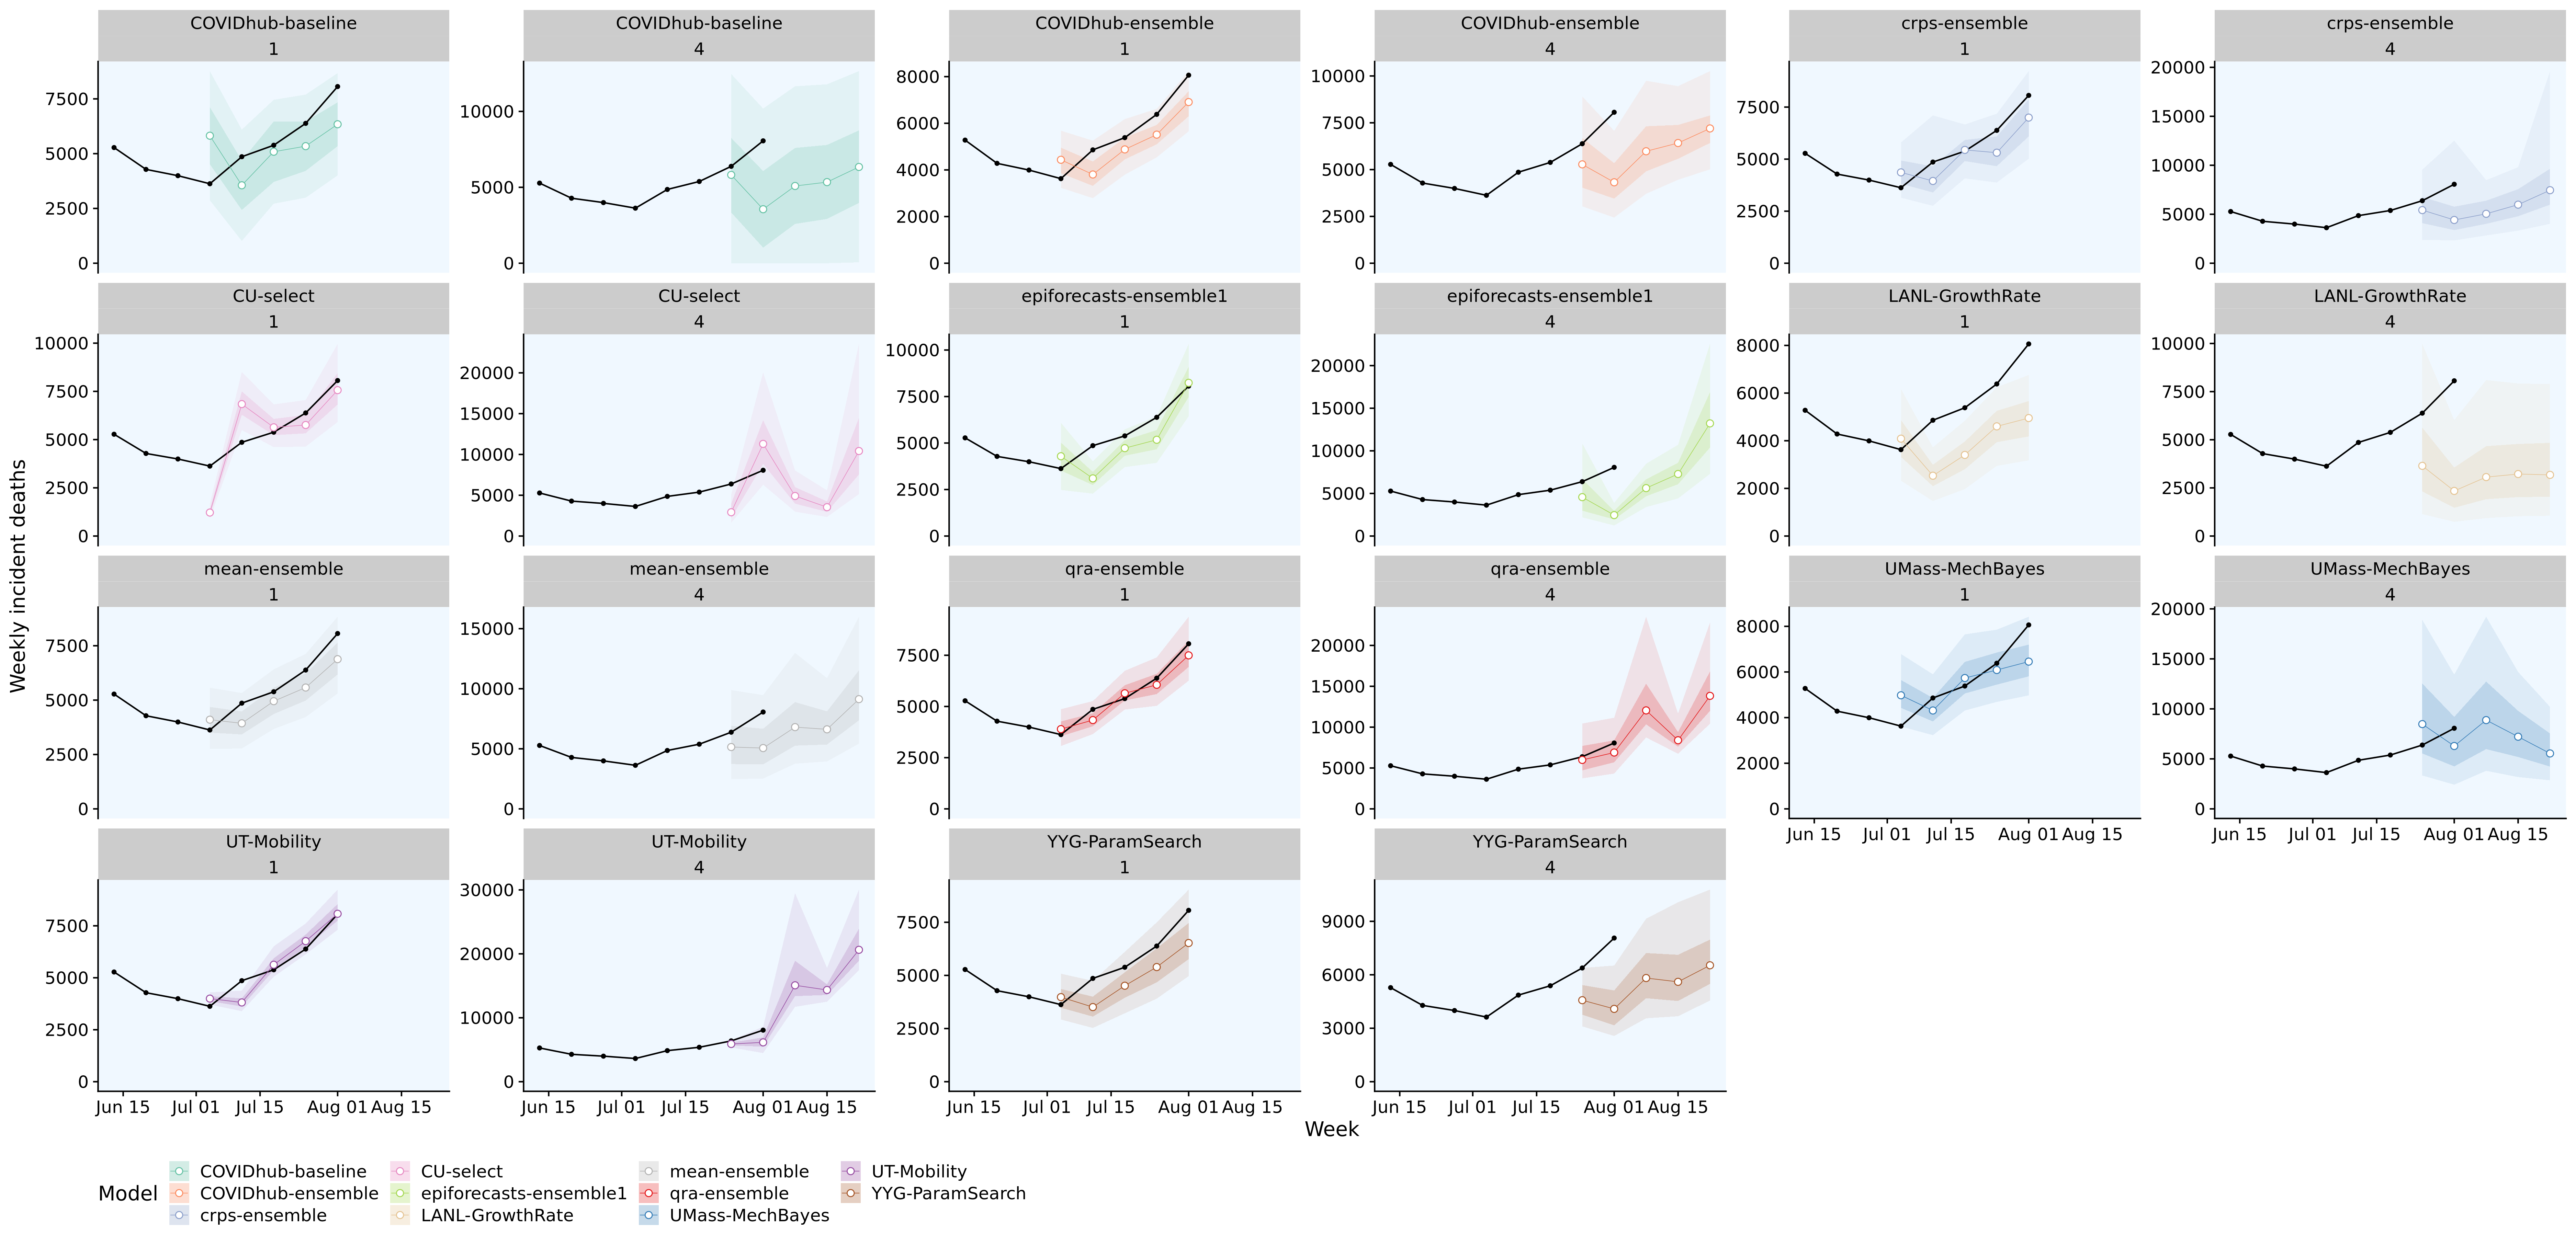
\includegraphics[width=1\linewidth]{../visualisation/chapter-5-results/US-forecast-1-4-wk-ahead} \caption{One week ahead forecasts for the US from all models}\label{fig:models-us}
\end{figure}

\hypertarget{summarised-scores}{%
\section{Summarised scores}\label{summarised-scores}}

We next turn to the aggregated scores from the different metrics and proper scoring. These help us to summarise the complexity and nuances of overall model performance with a few numbers. They are therefore a sensible starting point before going deeper into assessing model calibration and sharpness.

Figure \ref{fig:coloured-summarised-scores} shows the summarised scores for all eleven models from the metrics presented in Chapter \ref{evaluation}.

\begin{figure}
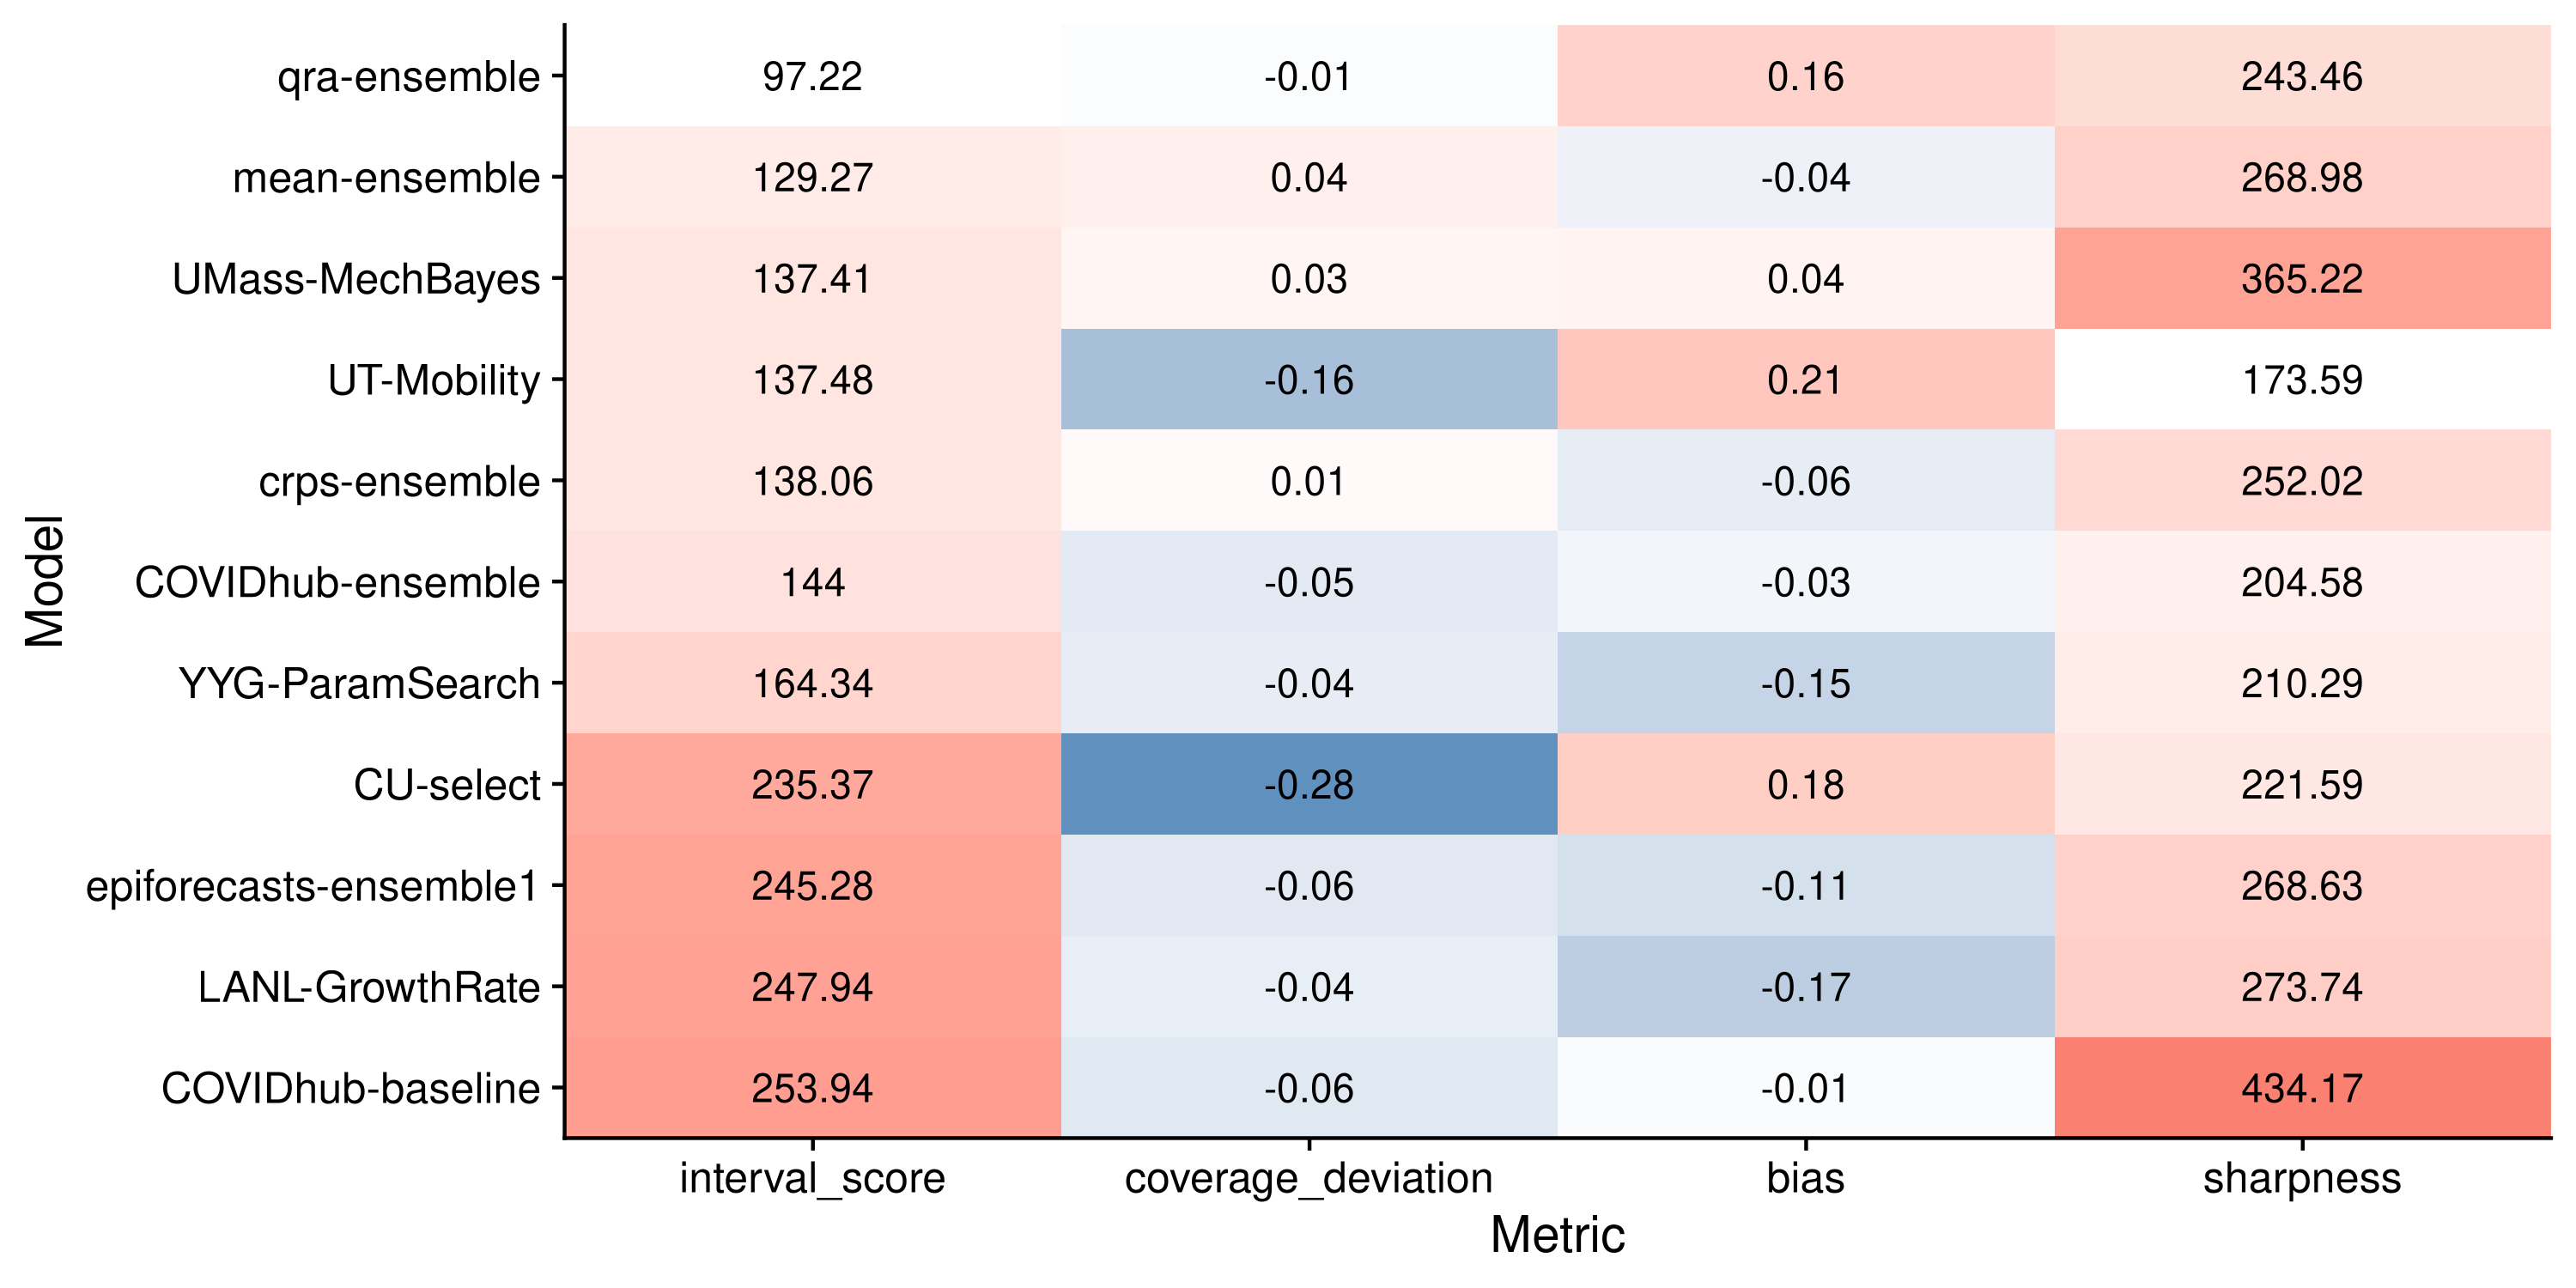
\includegraphics[width=1\linewidth]{../visualisation/chapter-5-results/coloured-summarised-scores} \caption{Colour coded summary of scores. Neutral / optimal values are shown in white, too low values in blue and too high values in red}\label{fig:coloured-summarised-scores}
\end{figure}

We can see that our quick visual ranking largely corresponds to the perfomance as judeged by the weighted interval score. The ensembles and UMassMechBayes rank at the top, while LANL-GrowthRate and UT-Mobility are ranked at the bottom. We don't, however, see the full picture from these aggregate scores. The epiforecasts-ensemble1, for example, does far worse than the UMass-MechBayes, even though both have similar values for coverage deviation, bias, absolute bias and sharpness. Absolute bias is included in Figure \ref{fig:coloured-summarised-scores}, as bias is aggregated over both positive and negative values and can therefore be misleading. We can see that the ranking is slightly different if we apply a log transformation to the weigthed interval score. This suggests that the average weighted interval score is heavily influenced by extreme values.

\hypertarget{correlation-between-metrics}{%
\subsection{Correlation between metrics}\label{correlation-between-metrics}}

To get a clearer understanding of how the different metrics relate, it seems sensible to look at the correlation between different metrics. Figure \ref{fig:correlation-map} shows the correlation matrix. This matrix also included log interval score and log sharpness, as both have very heavy tails and outliers. We can see that sharpness seems to have a surprisingly large influence on the weighted interval score. This may well be a feature of the weighted interval score. It cannot, however, be ruled out that the sharper models analysed here simply do better for other unknown reasons.

We can also see that bias and coverage deviation correlate strongly, which makes intuitive sense. A large absolute bias will lead to a lower empirical coverage which in turn results in a negative value for coverage deviation since coverage deviation is calculated as the difference between empirical coverage and desired nominal coverage. It is quite surprising to see, however that the correlation is nearly perfect and that coverage deviation and sharpness do not seem to correlate at all.

Other weightings for the weighted interval score may yield different relative influences of the other metrics. It could therefore be sensible to adapt the weights, e.g.~to get a stronger influence of the central intervals. This, however, is beyond the scope of this thesis. When interpreting the correlation, it is also important to note that the correlation matrix doesn't show `bias' and `calibration' as abstract concepts. Rather, it shows how the actual metrics chosen to measure bias and calibration correlate with the WIS - these may not actually cover all of what we would like them to cover.

\begin{figure}

{\centering 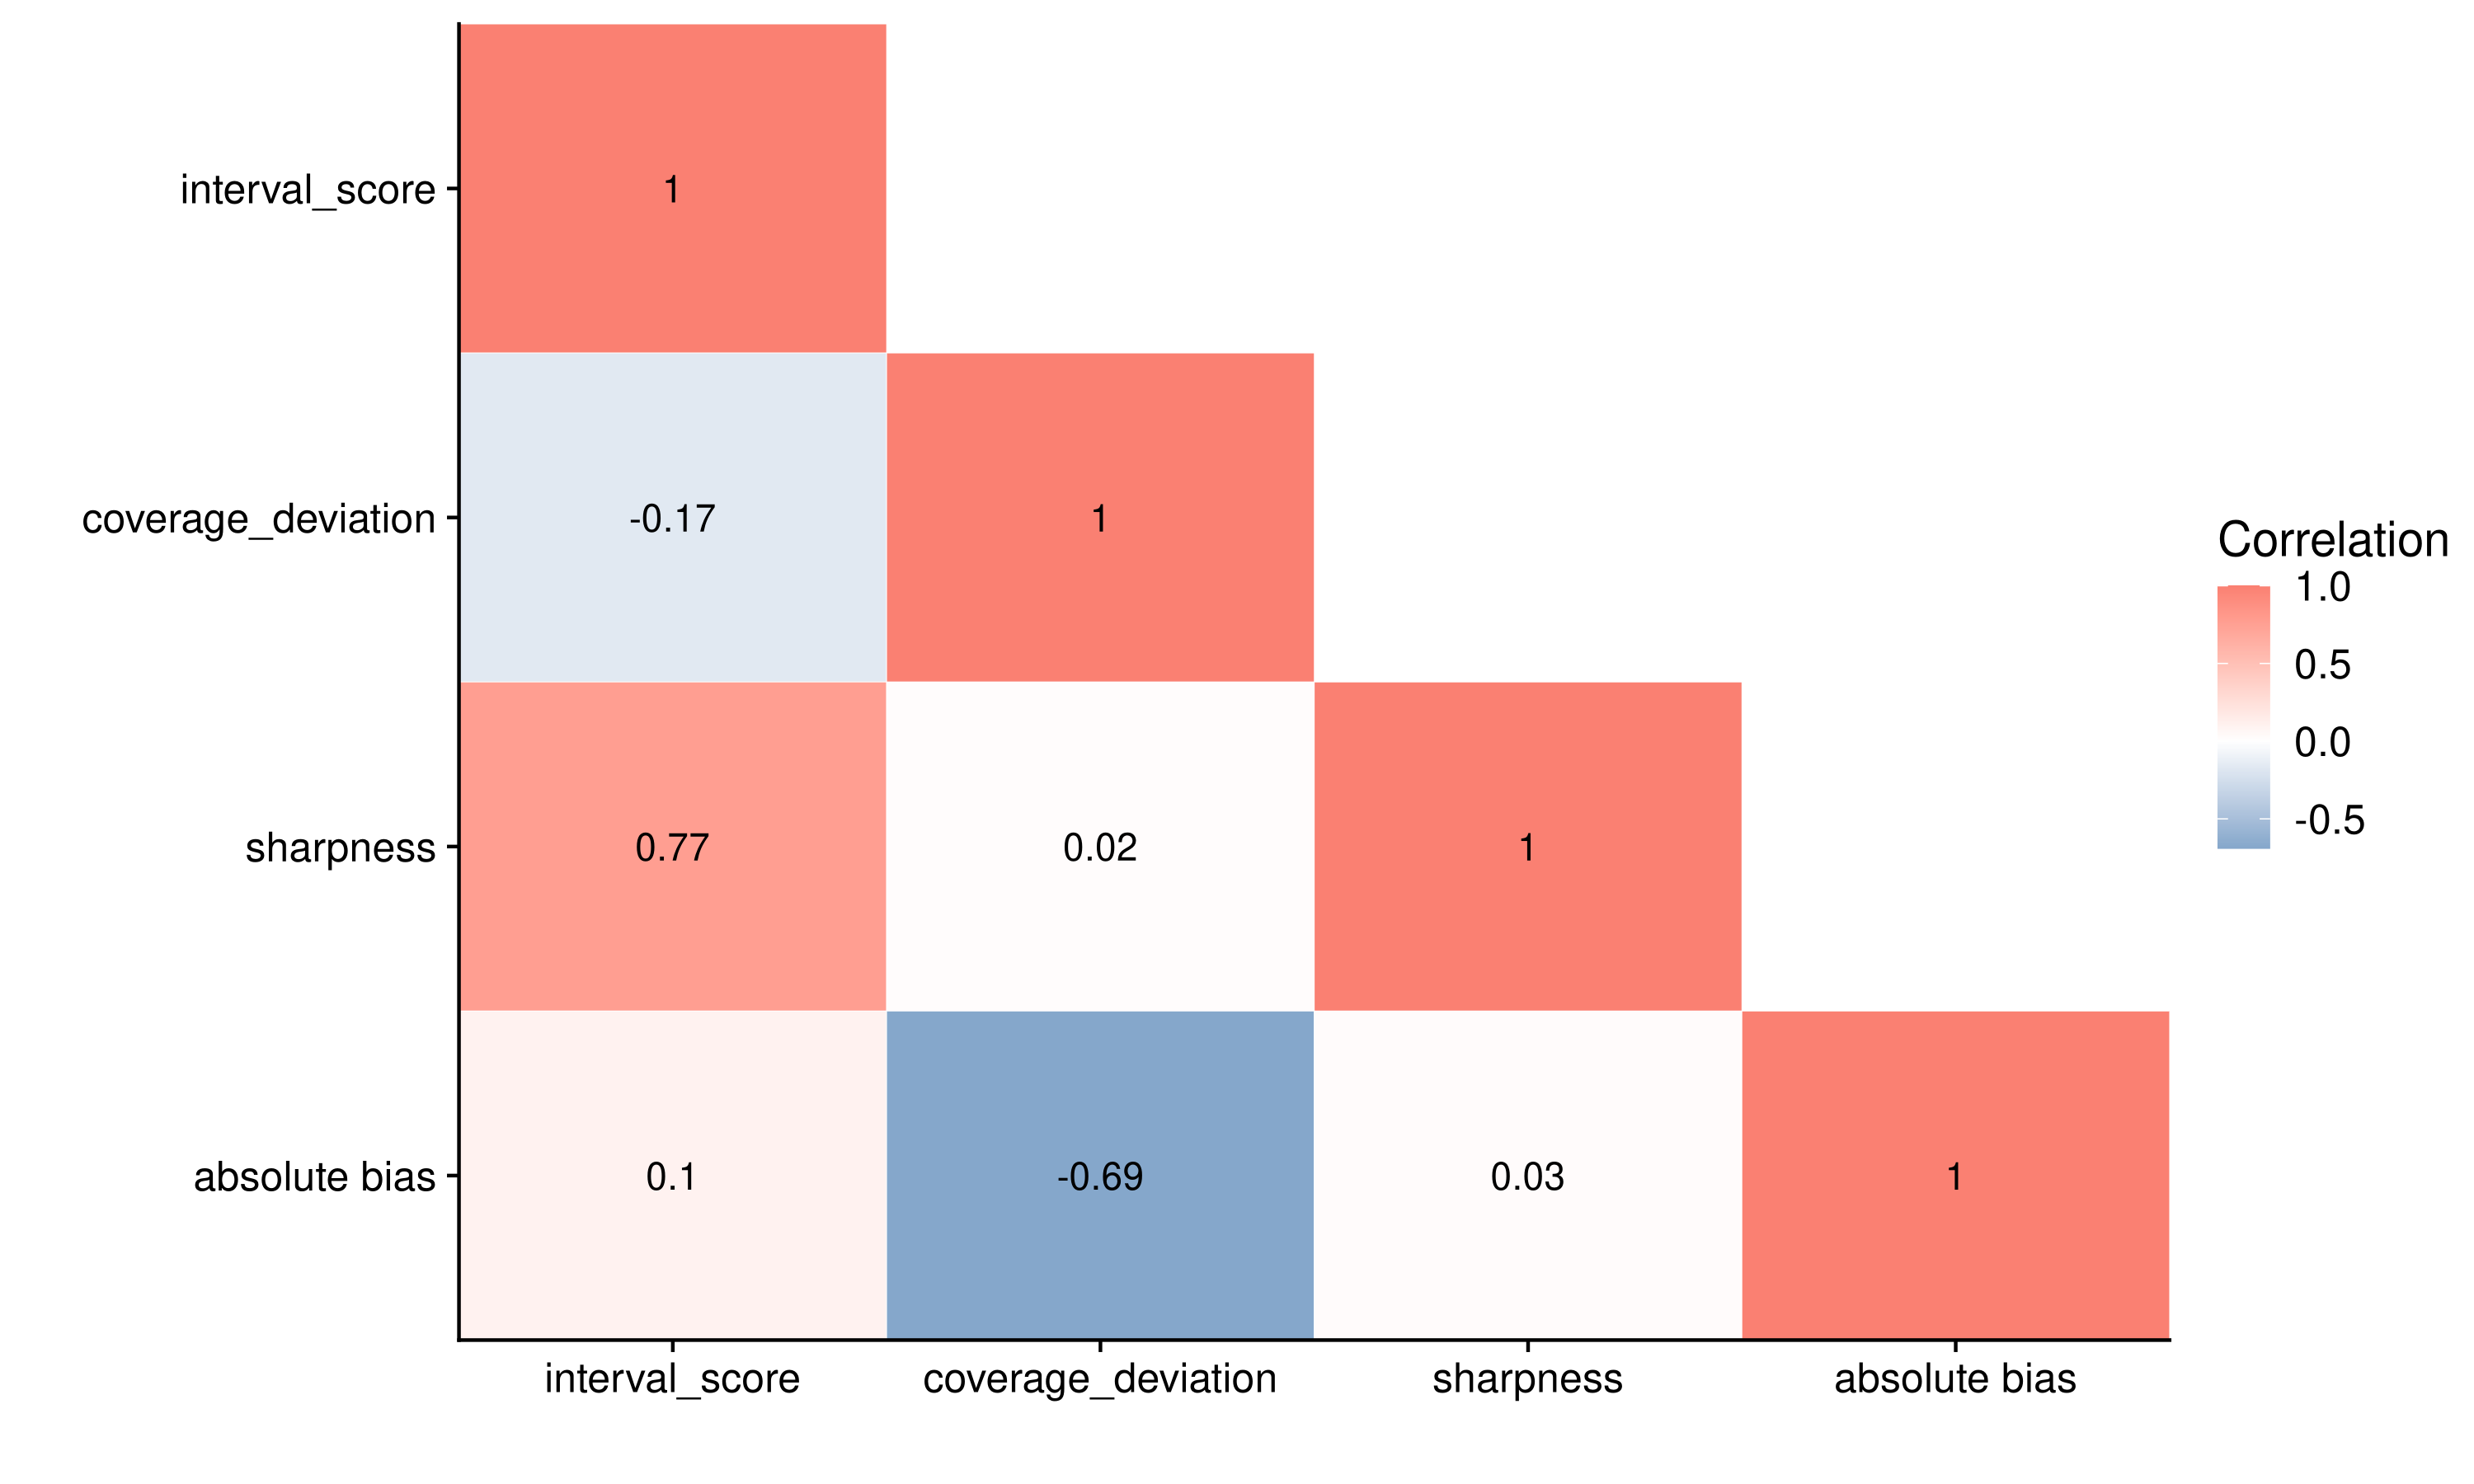
\includegraphics[width=1\linewidth]{../visualisation/chapter-5-results/correlation-map} 

}

\caption{Correlation between the different metrics }\label{fig:correlation-map}
\end{figure}

Figure \ref{fig:correlation-plot} shows a full correlation plot with all univariate and bivariate distributions. We can clearly see on the diagonal that sharpness and weighted interval score (WIS) have heavy tails. We can make some other interesting observations: A positive coverage deviation (i.e.~covering too much by stating too wide prediction intervals) is still associated with a lower WIS in the models analysed. We also see that while absolute bias and coverage deviation correlate with WIS, the variance is still immense.

\begin{figure}

{\centering 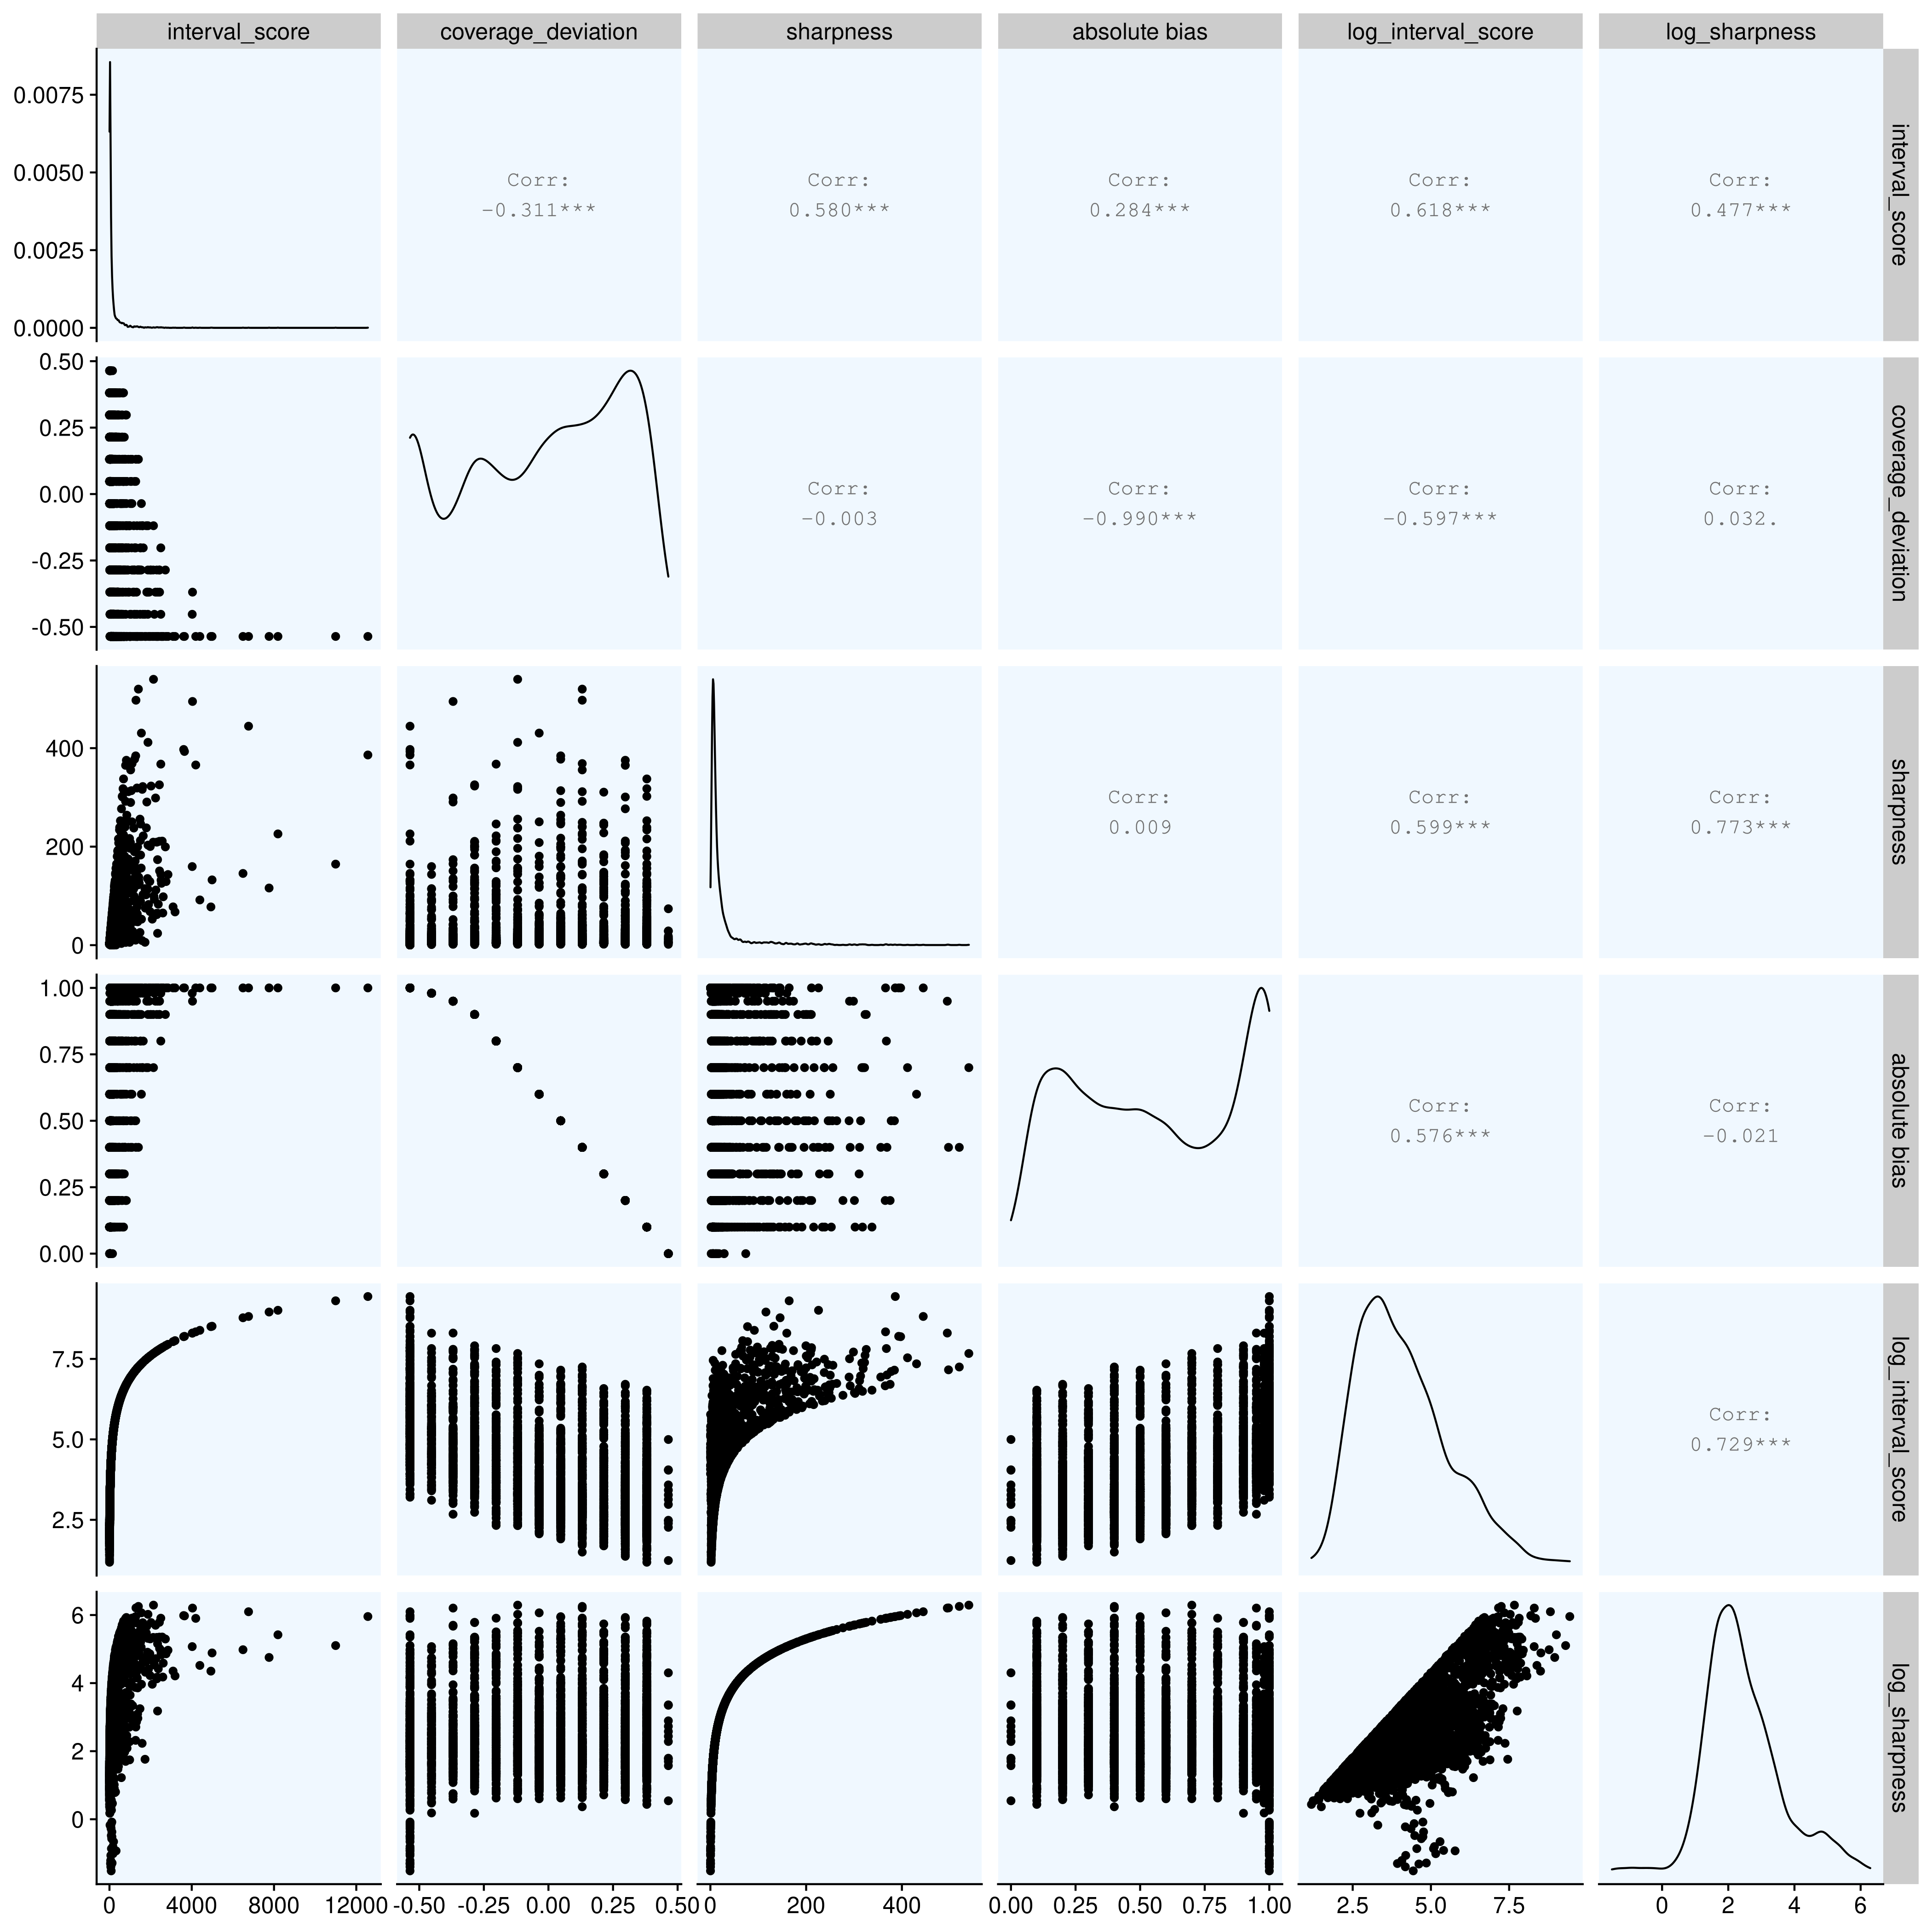
\includegraphics[width=1\linewidth]{../visualisation/chapter-5-results/corr-plot} 

}

\caption{Correlation plot that shows bivariate scatter plots for all evaluation metrics.}\label{fig:correlation-plot}
\end{figure}

Table \ref{tab:regression-wis-metrics} shows a quick regression of the log weighted interval score on absolute bias, coverage deviation and sharpness. All regressors have been standardised, so the effect size should be interpreted in terms of standard deviations. Coverage deviation and sharpness have the expected sign while absolute bias does not. As we have seen in Figure \ref{fig:correlation-map} bias and coverage deviation do correlate strongly, which might make estimation harder. Also for some reason it might be that coincidentally upwards biased models still performed well overall.

HOW DO I EXPLAIN THIS? MAYBE JUST DROP THE REGRESSION ALTOGETHER??

\begin{Shaded}
\begin{Highlighting}[]
\KeywordTok{lm}\NormalTok{(log\_scores }\OperatorTok{\textasciitilde{}}\StringTok{ }\NormalTok{abs\_bias\_std }\OperatorTok{+}\StringTok{ }\NormalTok{coverage\_deviation\_std }\OperatorTok{+}\StringTok{ }\NormalTok{log\_sharpness\_std, }
   \DataTypeTok{data =}\NormalTok{ unsummarised\_scores) }
\end{Highlighting}
\end{Shaded}

\begin{verbatim}
## 
## Call:
## lm(formula = log_scores ~ abs_bias_std + coverage_deviation_std + 
##     log_sharpness_std, data = unsum_scores)
## 
## Residuals:
##      Min       1Q   Median       3Q      Max 
## -1.73098 -0.12965 -0.00775  0.10938  3.06238 
## 
## Coefficients:
##                         Estimate Std. Error t value Pr(>|t|)    
## (Intercept)             4.080791   0.005803  703.22   <2e-16 ***
## abs_bias_std           -1.556420   0.040316  -38.60   <2e-16 ***
## coverage_deviation_std -2.406474   0.040328  -59.67   <2e-16 ***
## log_sharpness_std       1.061166   0.005824  182.20   <2e-16 ***
## ---
## Signif. codes:  0 '***' 0.001 '**' 0.01 '*' 0.05 '.' 0.1 ' ' 1
## 
## Residual standard error: 0.3328 on 3285 degrees of freedom
## Multiple R-squared:  0.943,	Adjusted R-squared:  0.943 
## F-statistic: 1.812e+04 on 3 and 3285 DF,  p-value: < 2.2e-16
\end{verbatim}

\label{tab:regression-wis-metrics}Regression of the log weighted interval score on the (standardised) absolute bias, coverage deviation and sharpness.

\hypertarget{scores-by-subgroups}{%
\subsection{Scores by subgroups}\label{scores-by-subgroups}}

Proceeding further we can break down the performance by different subgroups such as states, forecast horizons, and interval ranges to obtain a better understanding of what drives differences in the overall model scores. Figure \ref{fig:heatmap-performance} gives an overview of the model performance as judged by the WIS for every state. The colour indicates the overall rank that the model achieved in a given state. States are sorted from highest average interval score to lowest to illustrate contributions from different states. When averaging over different states, the overall weighted interval score is heavily influenced by few very large values. Large WIS values are most common in states with high case numbers (as small relative errors translate to large absolute deviations) and for larger horizons (as uncertainty grows).

MAYBE PLOT OF AVERAGE WIS VS NUMBER OF CASES OR / AND HORIZON

\begin{figure}
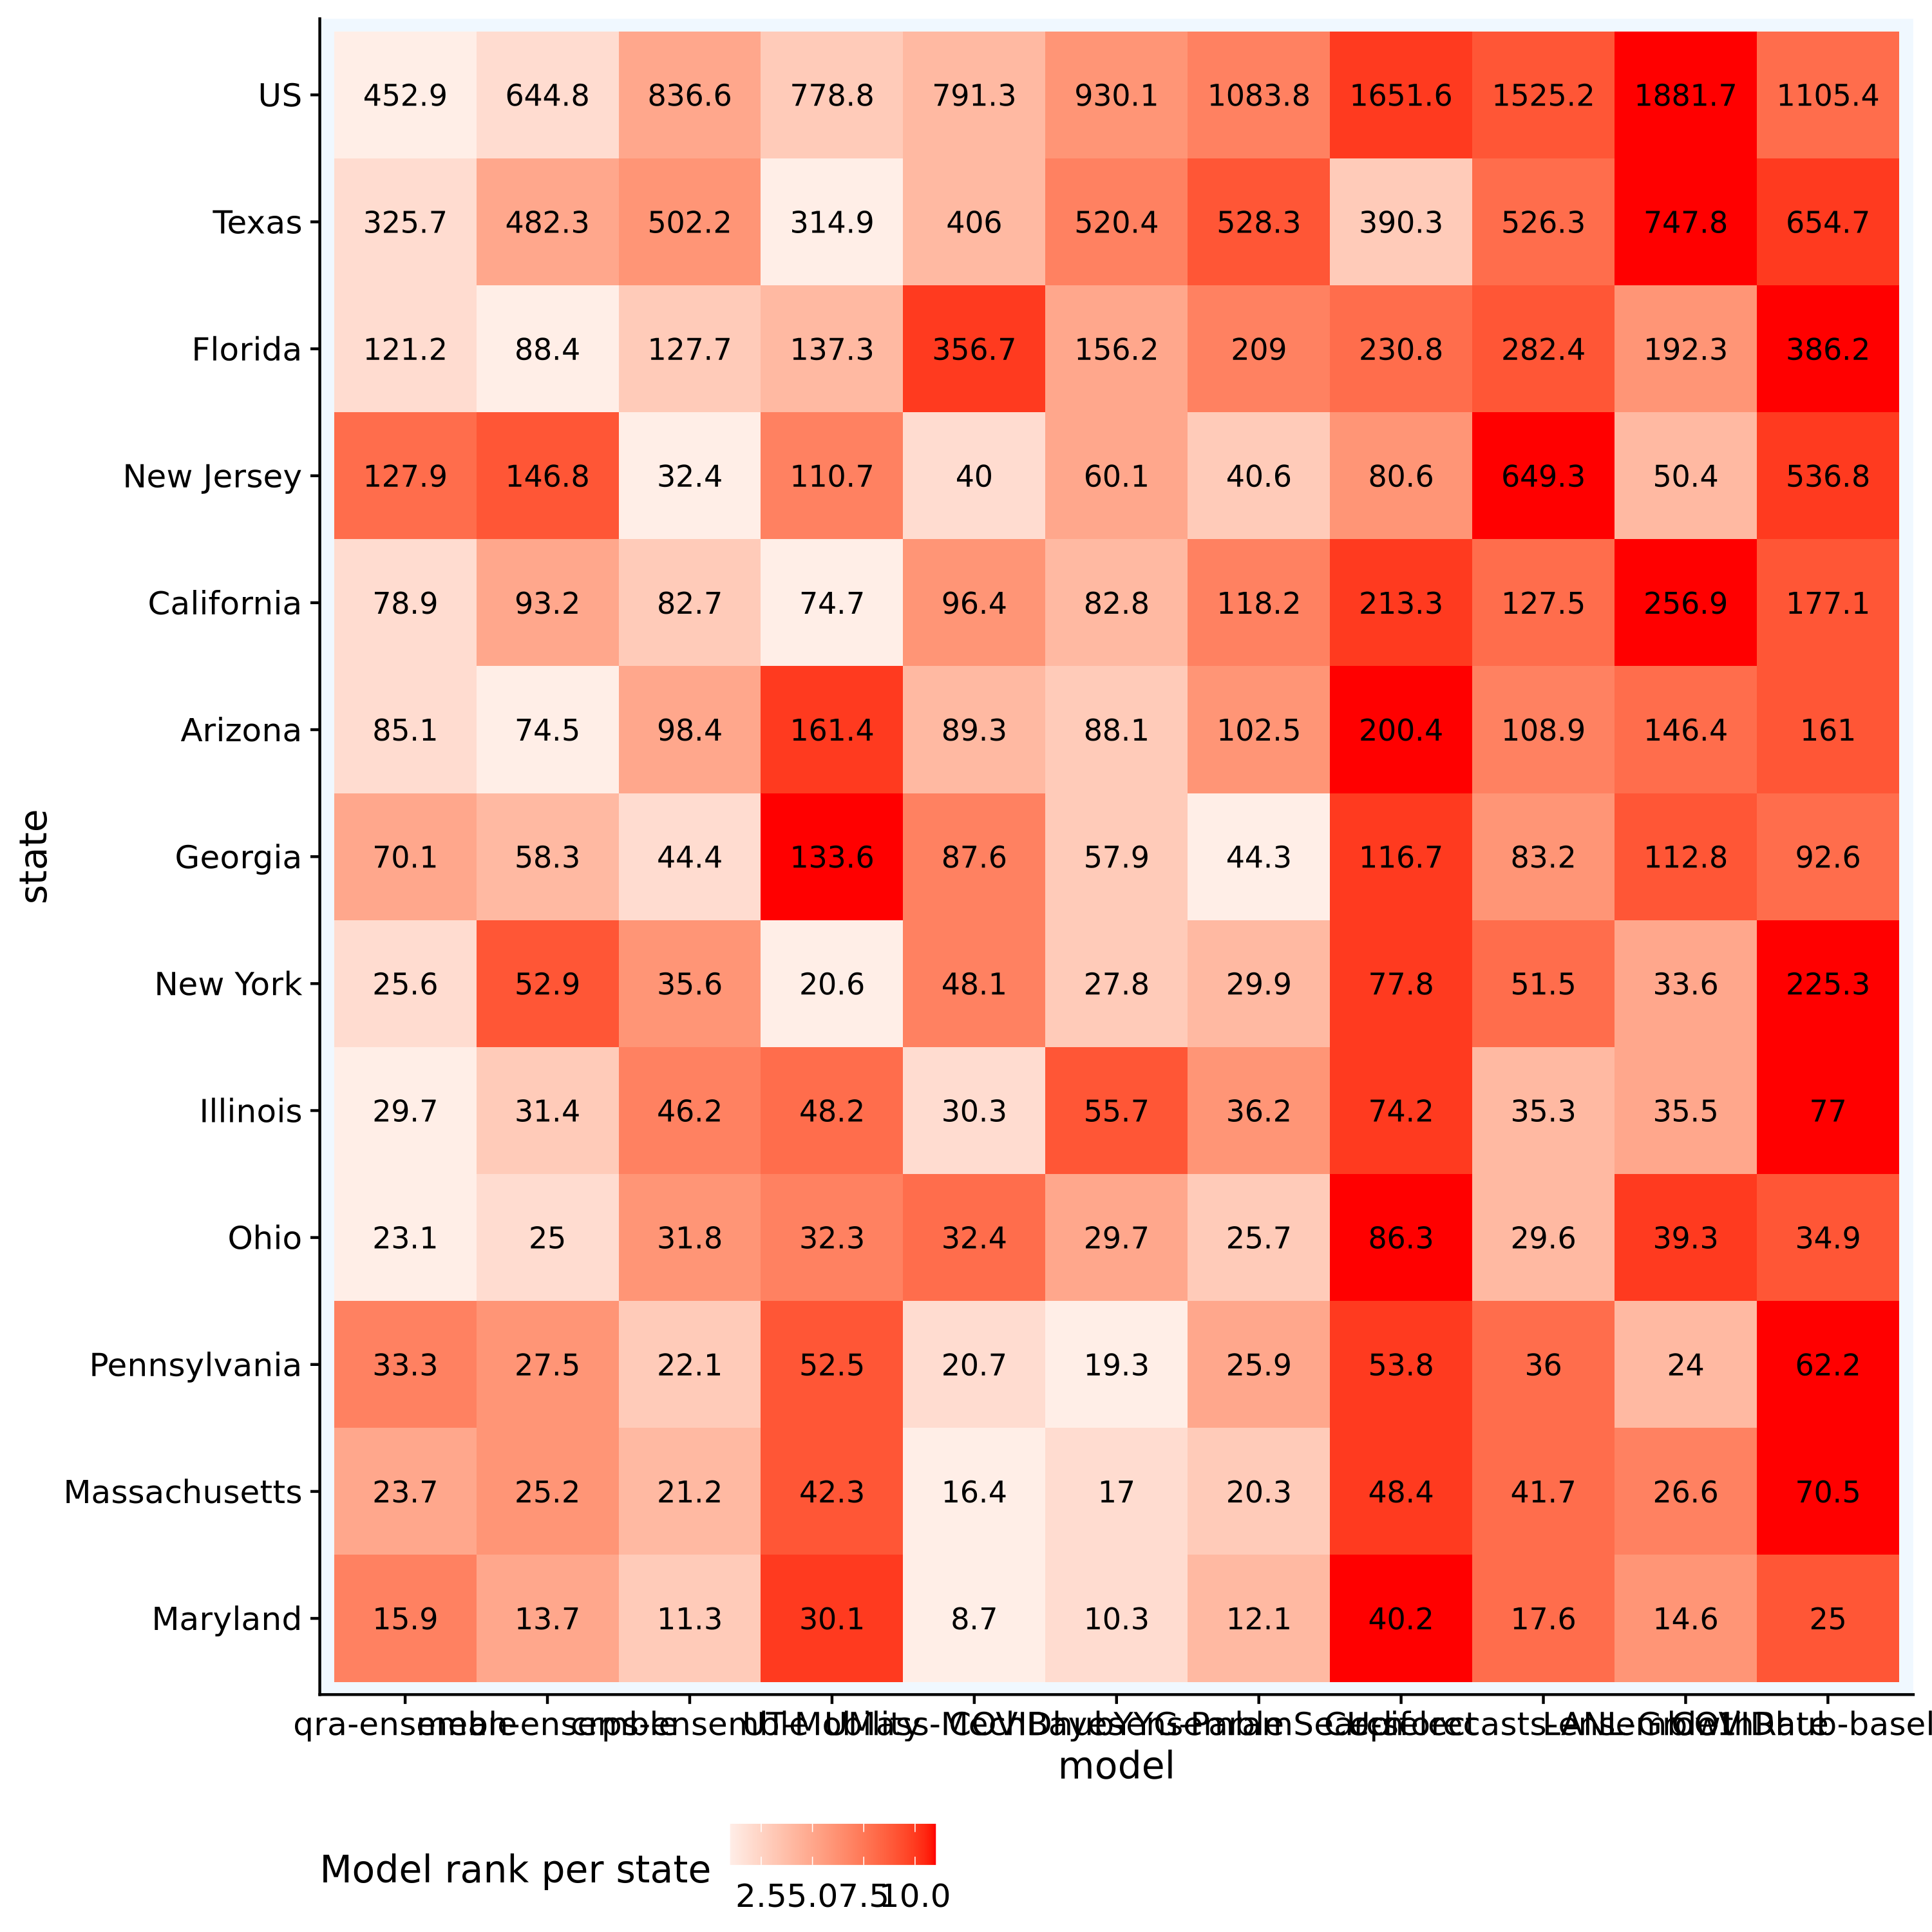
\includegraphics[width=1\linewidth]{../visualisation/chapter-5-results/heatmap-model-scores} \caption{Heatmap with the average of the weighted interval score over all horizons, states and forecast dates. The colouring indicates the rank of the model per state}\label{fig:heatmap-performance}
\end{figure}

Figure \ref{fig:heatmap-performance-horizon} shows performance over horizons instead of states. The colouring now indicates how much higher a score is relative to the score achieved for one-week-ahead forecasts by the model. Models are again sorted from lowest to highest average weighted interval score. The plot highlights how much general model performance is affected by the accuracy of long term forecasts rather than short term forecasts. The qra-ensemble for example does very well for one-week-ahead forecasts, but its performance deteriorates substantially further ahead into the future.

\begin{figure}
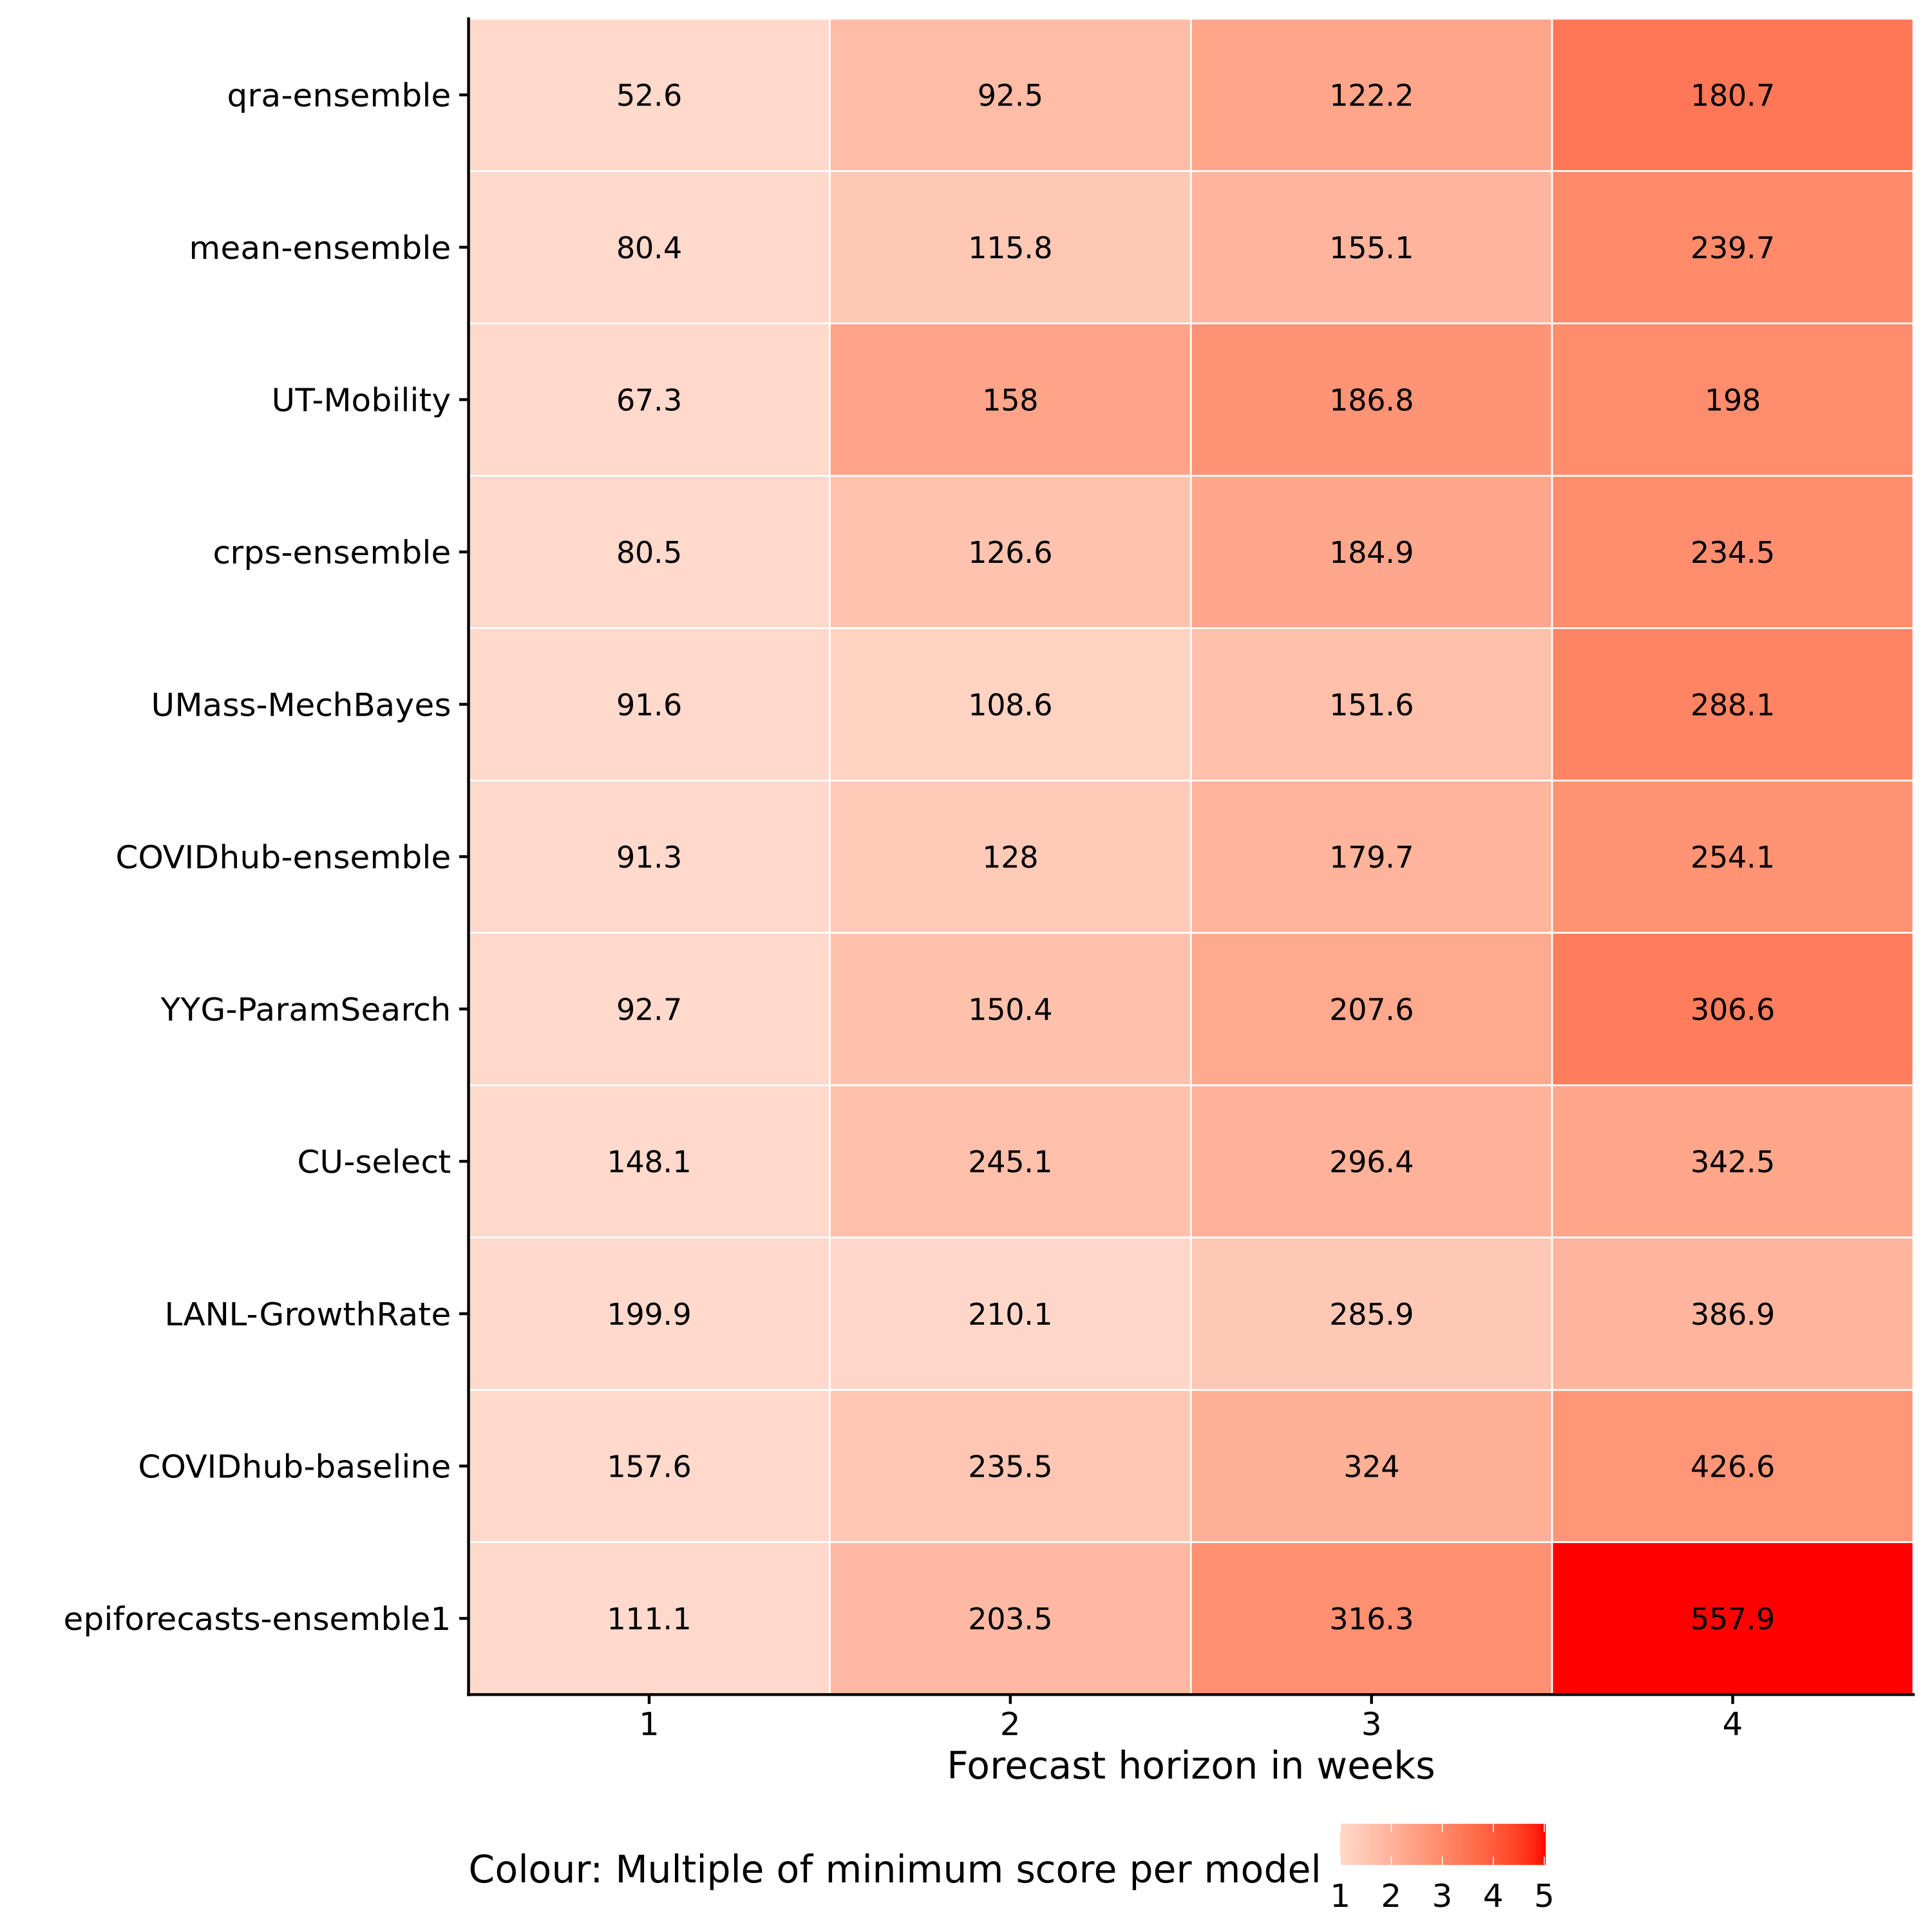
\includegraphics[width=1\linewidth]{../visualisation/chapter-5-results/heatmap-model-scores-horizon} \caption{Heatmap with the average of the weighted interval score across all states and forecast dates. The colouring indicates how much higher a score is relative to the lowest average score achieved by a model}\label{fig:heatmap-performance-horizon}
\end{figure}

To understand the composition of the weighted interval score better we can also look at the contributions from different interval ranges to the overall WIS. Figure \ref{fig:scores-ranges} shows that the WIS as implemented here seems to be more strongly influenced by the inner prediction intervals (small interval range) than the outer intervals (large range). Note again that other weightings are possible for the weighted interval score.

\begin{figure}
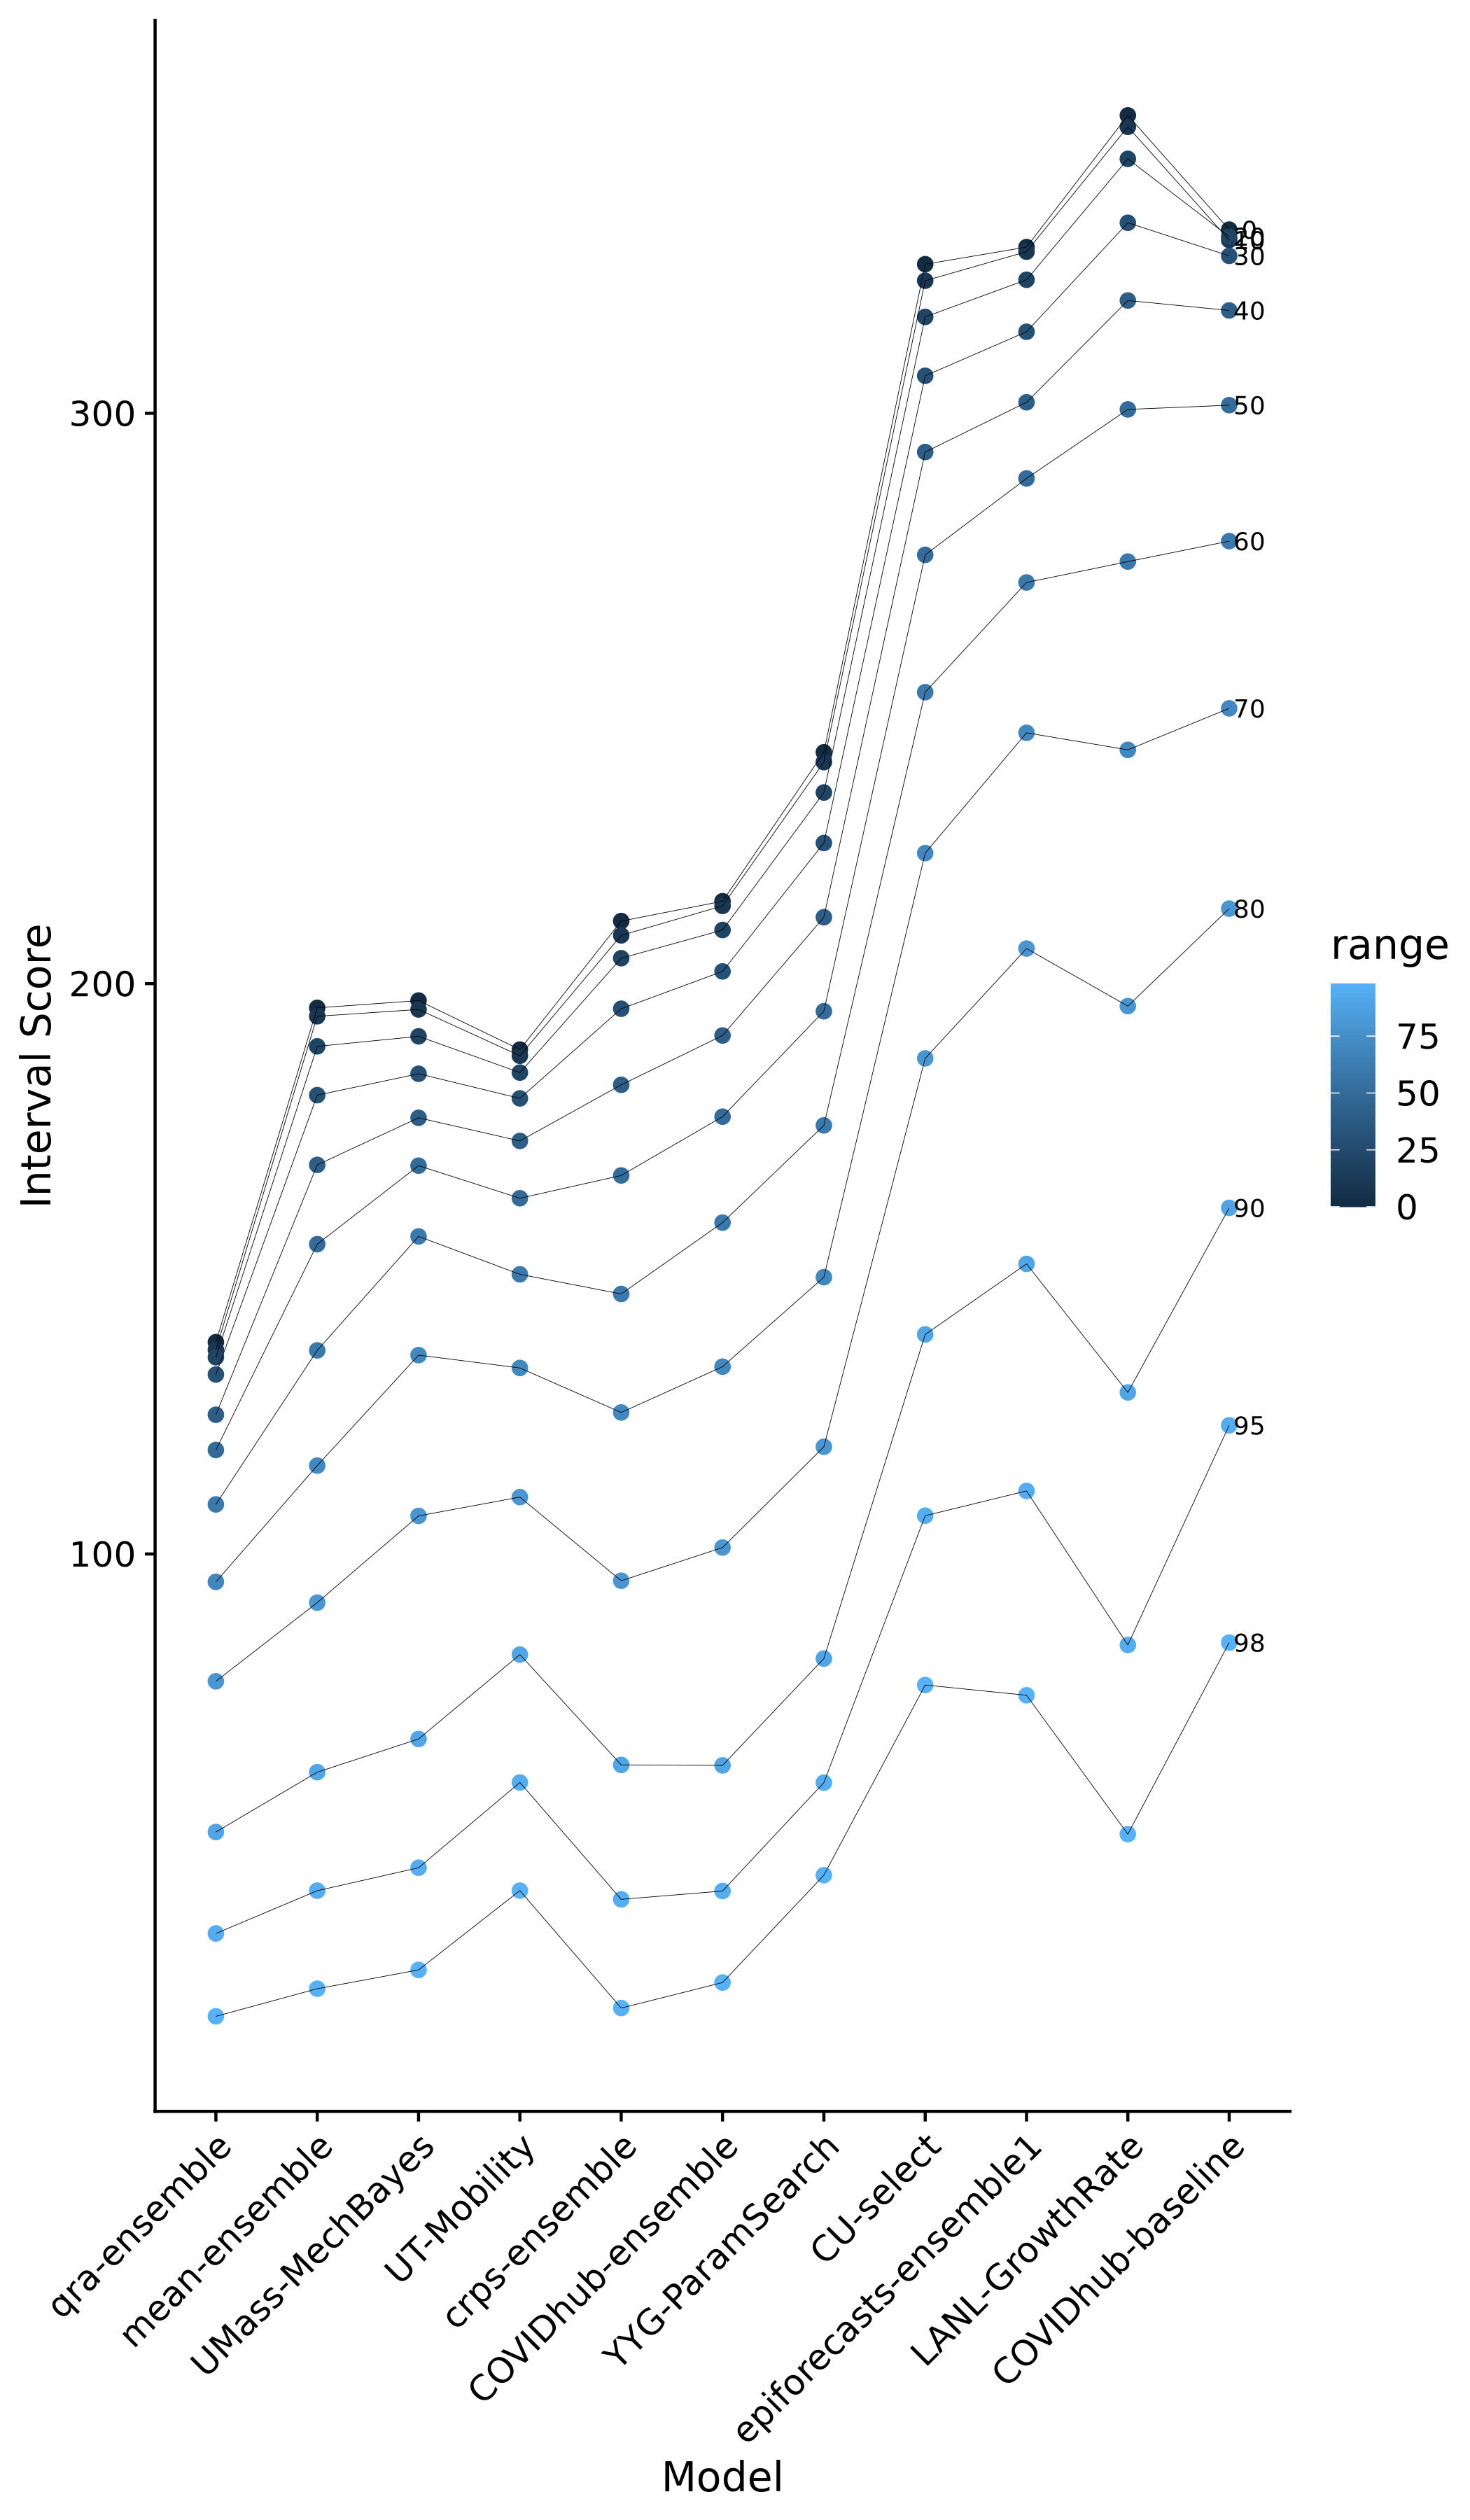
\includegraphics[width=1\linewidth]{../visualisation/chapter-5-results/scores-by-range} \caption{Interval scores across all states and forecast dates and horizons for different interval ranges}\label{fig:scores-ranges}
\end{figure}

After having examined the aggregated scores we can now move to visualise and analyse calibration and sharpness in detail.

\hypertarget{assessing-calibration}{%
\section{Assessing Calibration}\label{assessing-calibration}}

\hypertarget{bias}{%
\subsection{Bias}\label{bias}}

Just as we did with in Chapter \ref{evaluation}, we start our analysis of calibration with bias. For the purpose of model improvement it seems most useful to compare the evolution of bias over time with the actual predictions and observations. With the help of this comparison we can obtain insights regarding the particular situations that cause models to biased or not. While this is of course unfeasible to do for all eleven models, Figure \ref{fig:bias-ensemble} shows one-week-ahead predictions and bias for the three ensemble models in the six locations with the highest average WIS. We see that all models make very similar predictions. The qra-ensemble seems to have a slight tendency for higher bias values, but this is hard to infer just from looking at the plots.
All models seems to have some difficulties with picking up rapid changes in trends. This is especially pronounced in Texas. We can see that models seem to overpredict when deaths are increasing (Arizona, Texas) and seem to underpredict when cases are decreasing (New Jersey, last two weeks in Arizona).

Looking at the plot we can digress a bit and make a second unrelated observation regarding the crps-ensemble model: Plots of New Jersey (and maybe Florida) show that the model sometimes produces very large spikes in uncertainty. This can probably be attributed to the loss of precision that results from the sampling in the crps model aggregation progress. If we look back at the PLOT IN CHAPTER MODEL AGGREGATION, we can probably attribute this to the loss of precision due to sampling. We saw IN THE PLOT that samples from the gamma distribution tend to have much larger tails than the actual distribution.

\begin{figure}
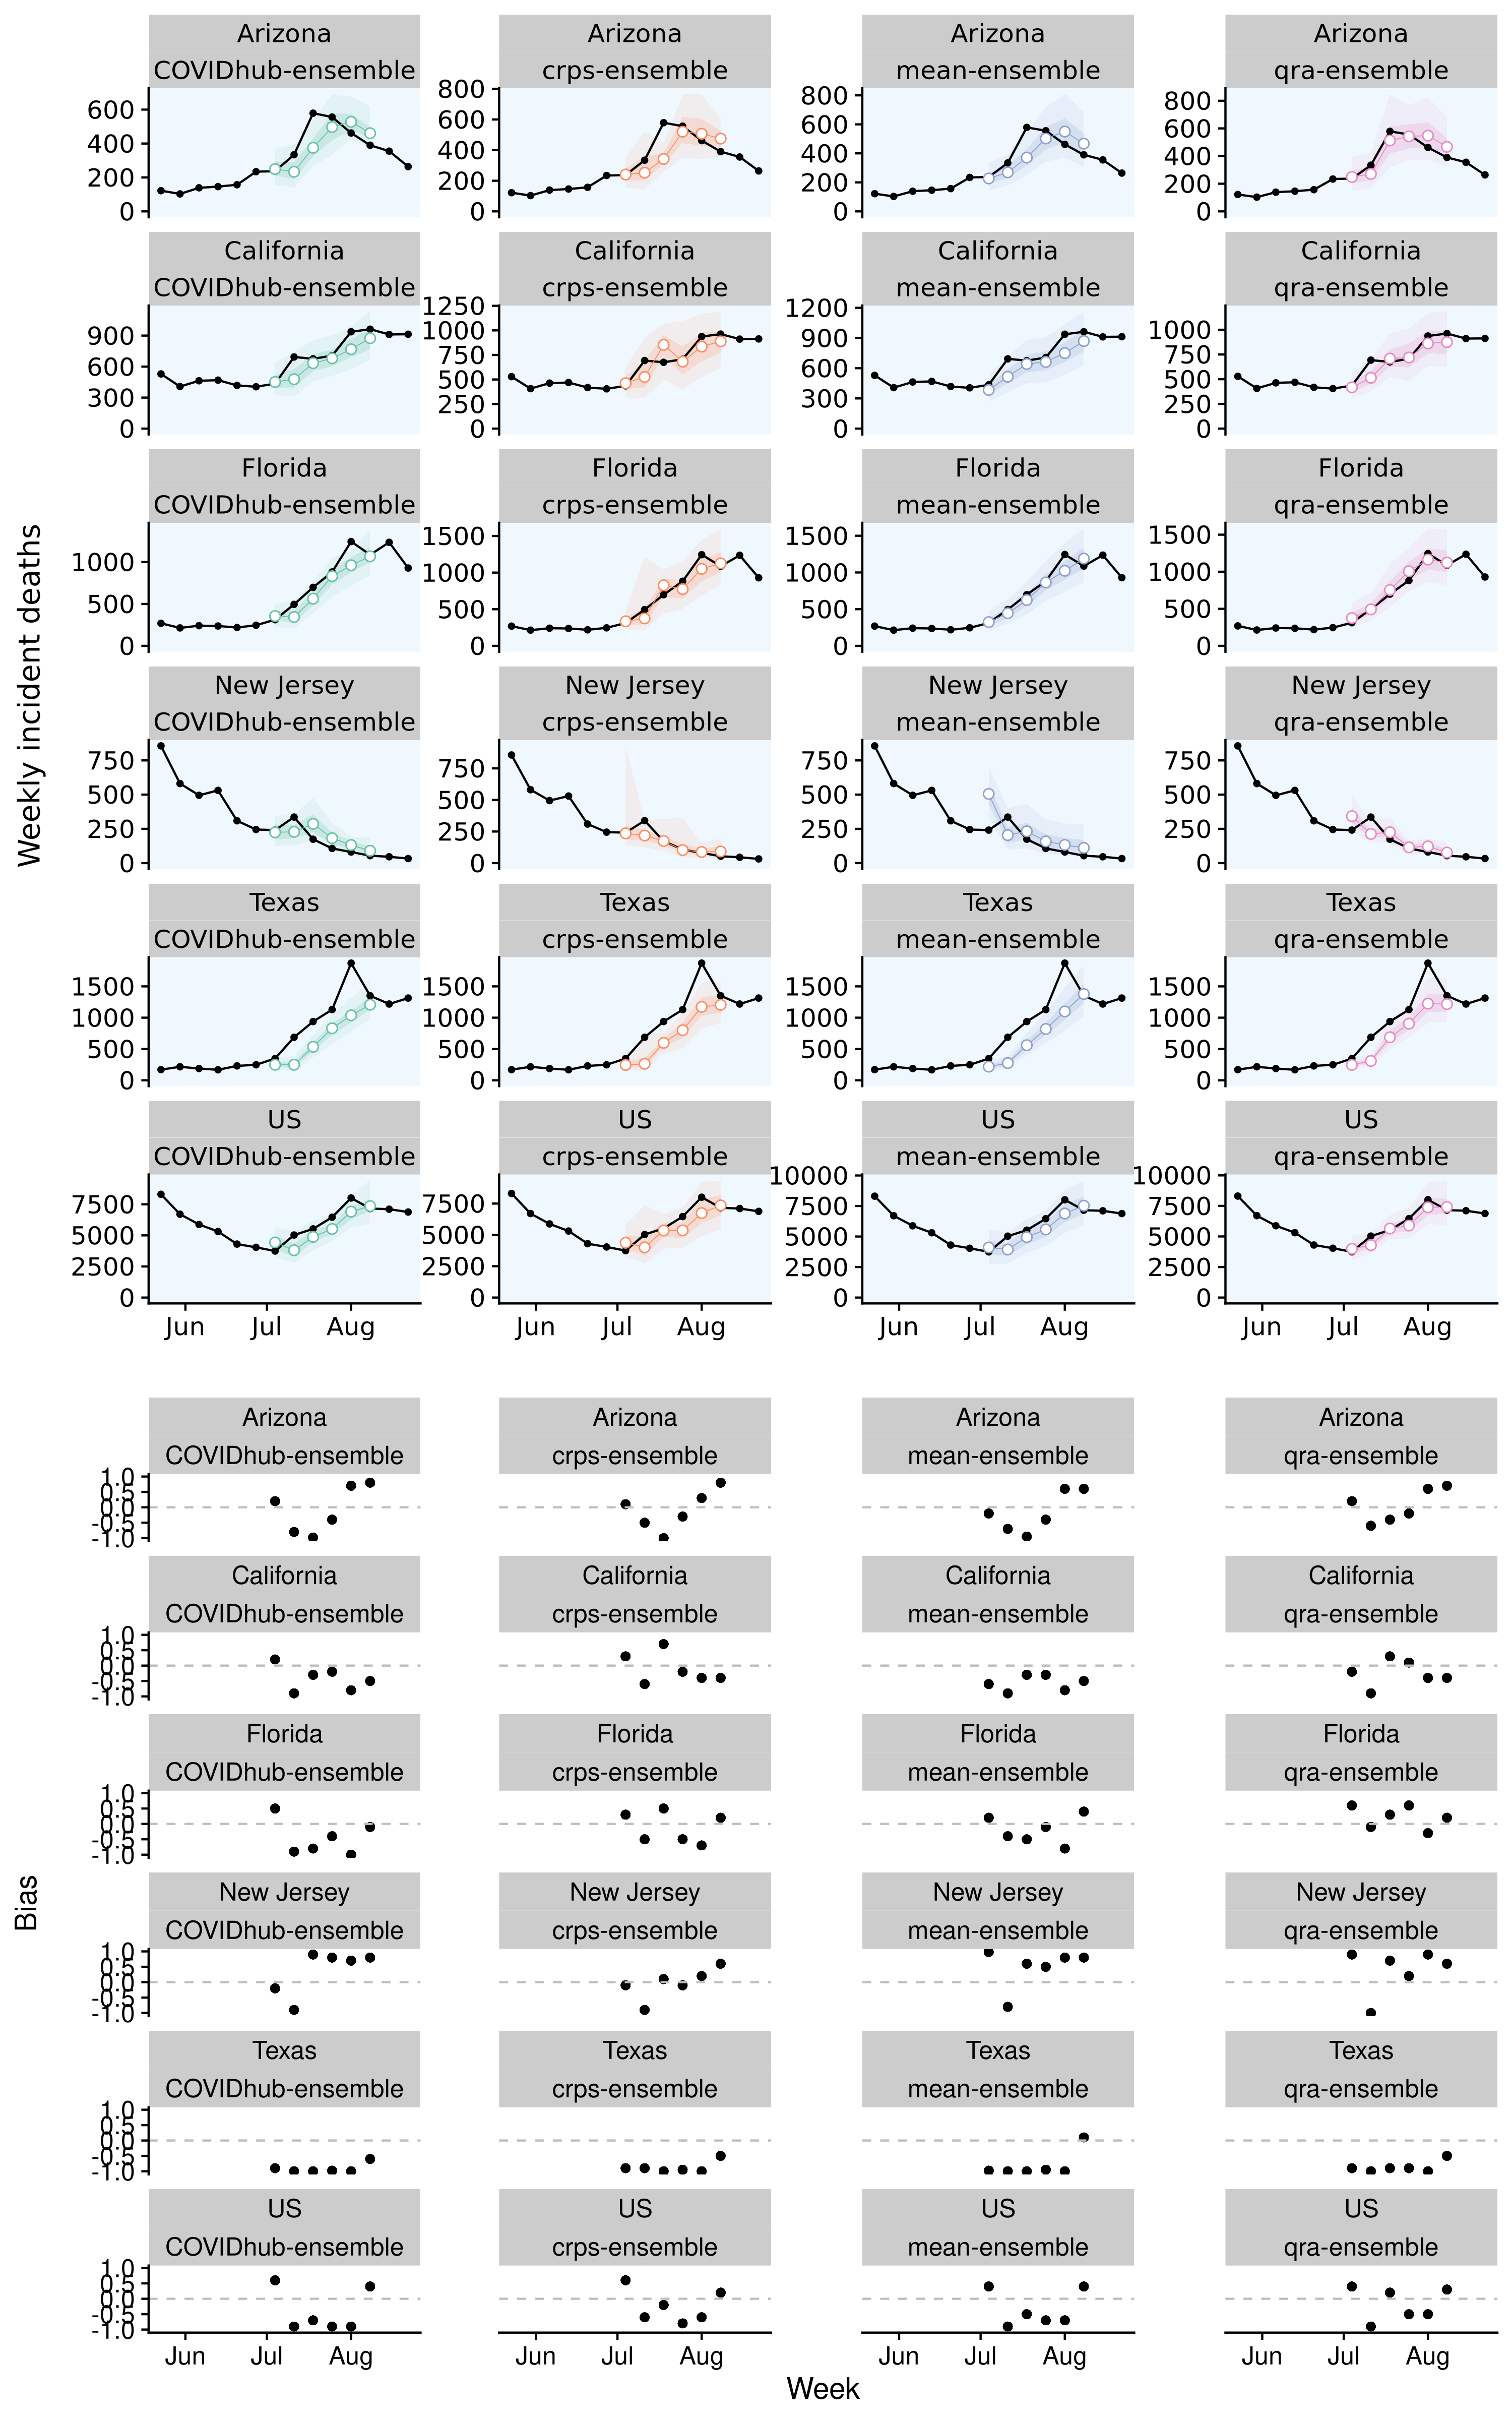
\includegraphics[width=1\linewidth]{../visualisation/chapter-5-results/bias_ensemble} \caption{Observations and predictions (top) as well as bias (bottom) for the YYG-ParamSearch model in the six states that exhibited the largest absolute bias.}\label{fig:bias-ensemble}
\end{figure}

\hypertarget{bias-by-subgroups}{%
\subsubsection{Bias by subgroups}\label{bias-by-subgroups}}

horizons, states

Figure \ref{fig:bias-all} shows bias for all models over different forecast horizons. We see that absolute bias tends to be a bit larger for greater horizons (though maybe not as much larger as expected) and that bias tends to be a slightly larger for worse ranked models. Overall, however, no really clear picture emerges.

\begin{figure}
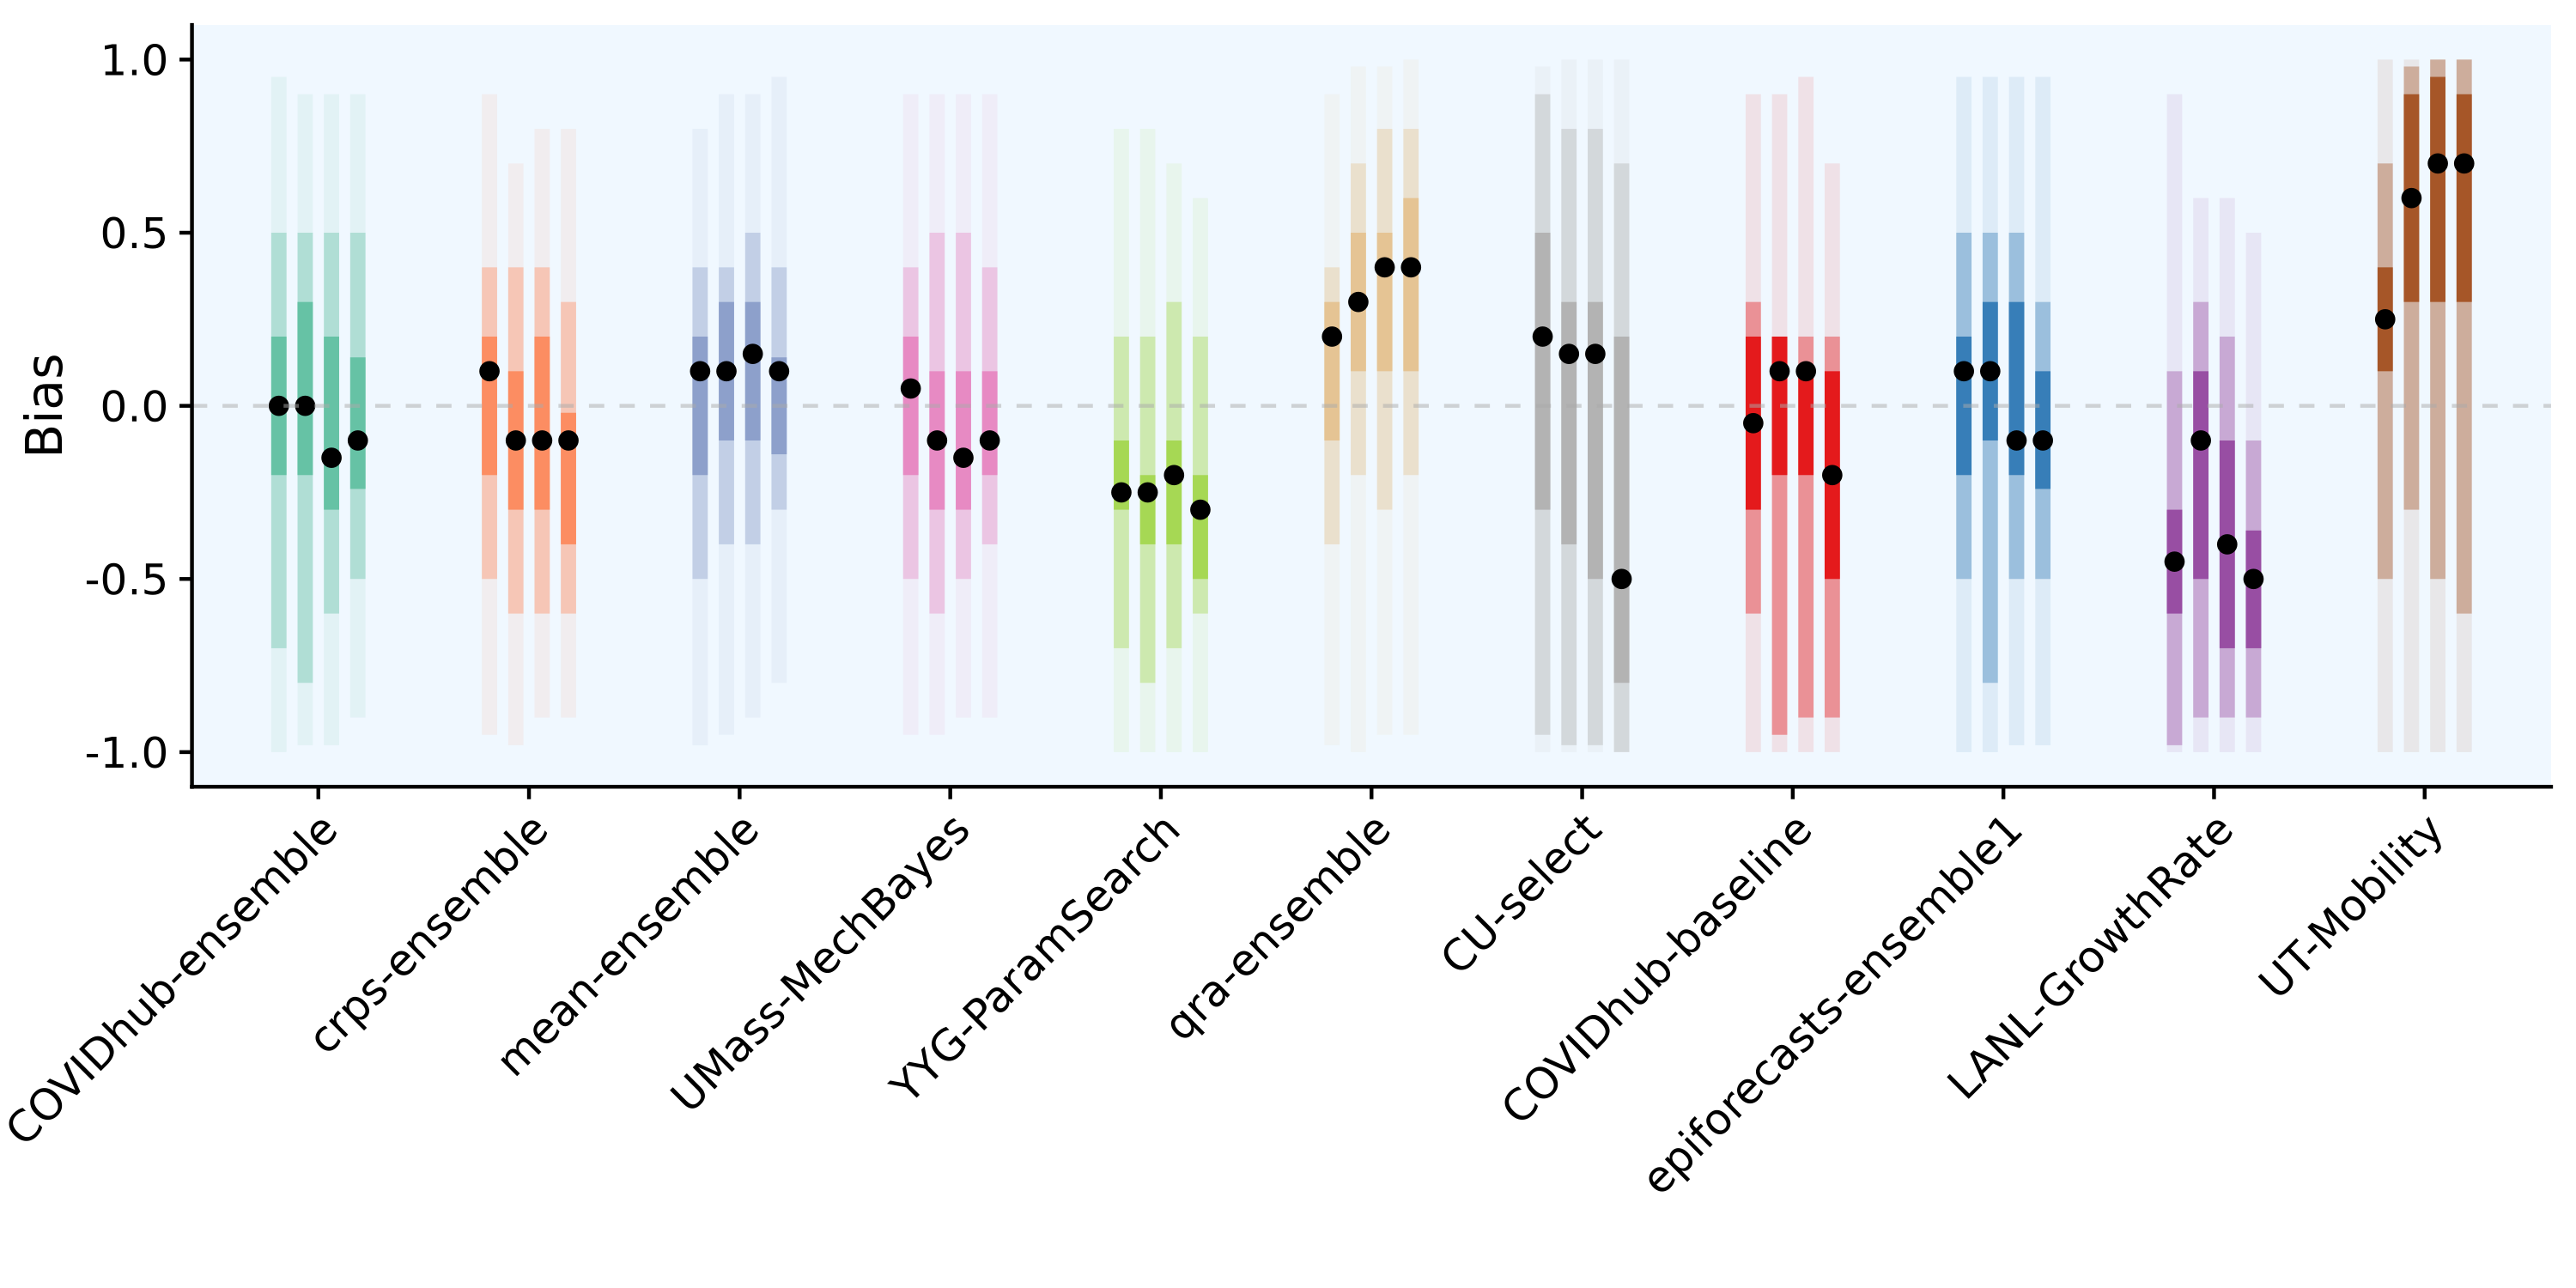
\includegraphics[width=1\linewidth]{../visualisation/chapter-5-results/bias-horizons} \caption{Bias for all models and different horizons. The black dot denotes the median bias, the black square the mean bias and different colour shadings show the 20, 40, and 90 percent intervals of all observed quantile values. Models are again ordered according to their overall performance by WIS.}\label{fig:bias-all}
\end{figure}

BIAS IN DIFFERENT STATES?

\hypertarget{coverage}{%
\subsection{Coverage}\label{coverage}}

We next turn to examine coverage. Figure \ref{fig:interval-coverage-all} shows the empirical interval coverage for all eleven models. We see that some models (especially CU-select and UT-mobility) have problems with calibration. The COVIDhub-baseline model is an interesting case. While the aggregated coverage deviation score in Figure \ref{fig:coloured-summarised-scores} looked very good, we can now conclude from this plot that the COVIDhub-baseline is not well calibrated. It instead is covering too much by its inner prediction intervals, but too little by its outer intervals. The epiforecasts-ensemble1, the qra-ensemble and especially the COVIDhub-ensemble seem to do best in terms of interval coverage. Looking only at interval coverage plots, however, does not tell us where the lack of coverage comes from.

\begin{figure}
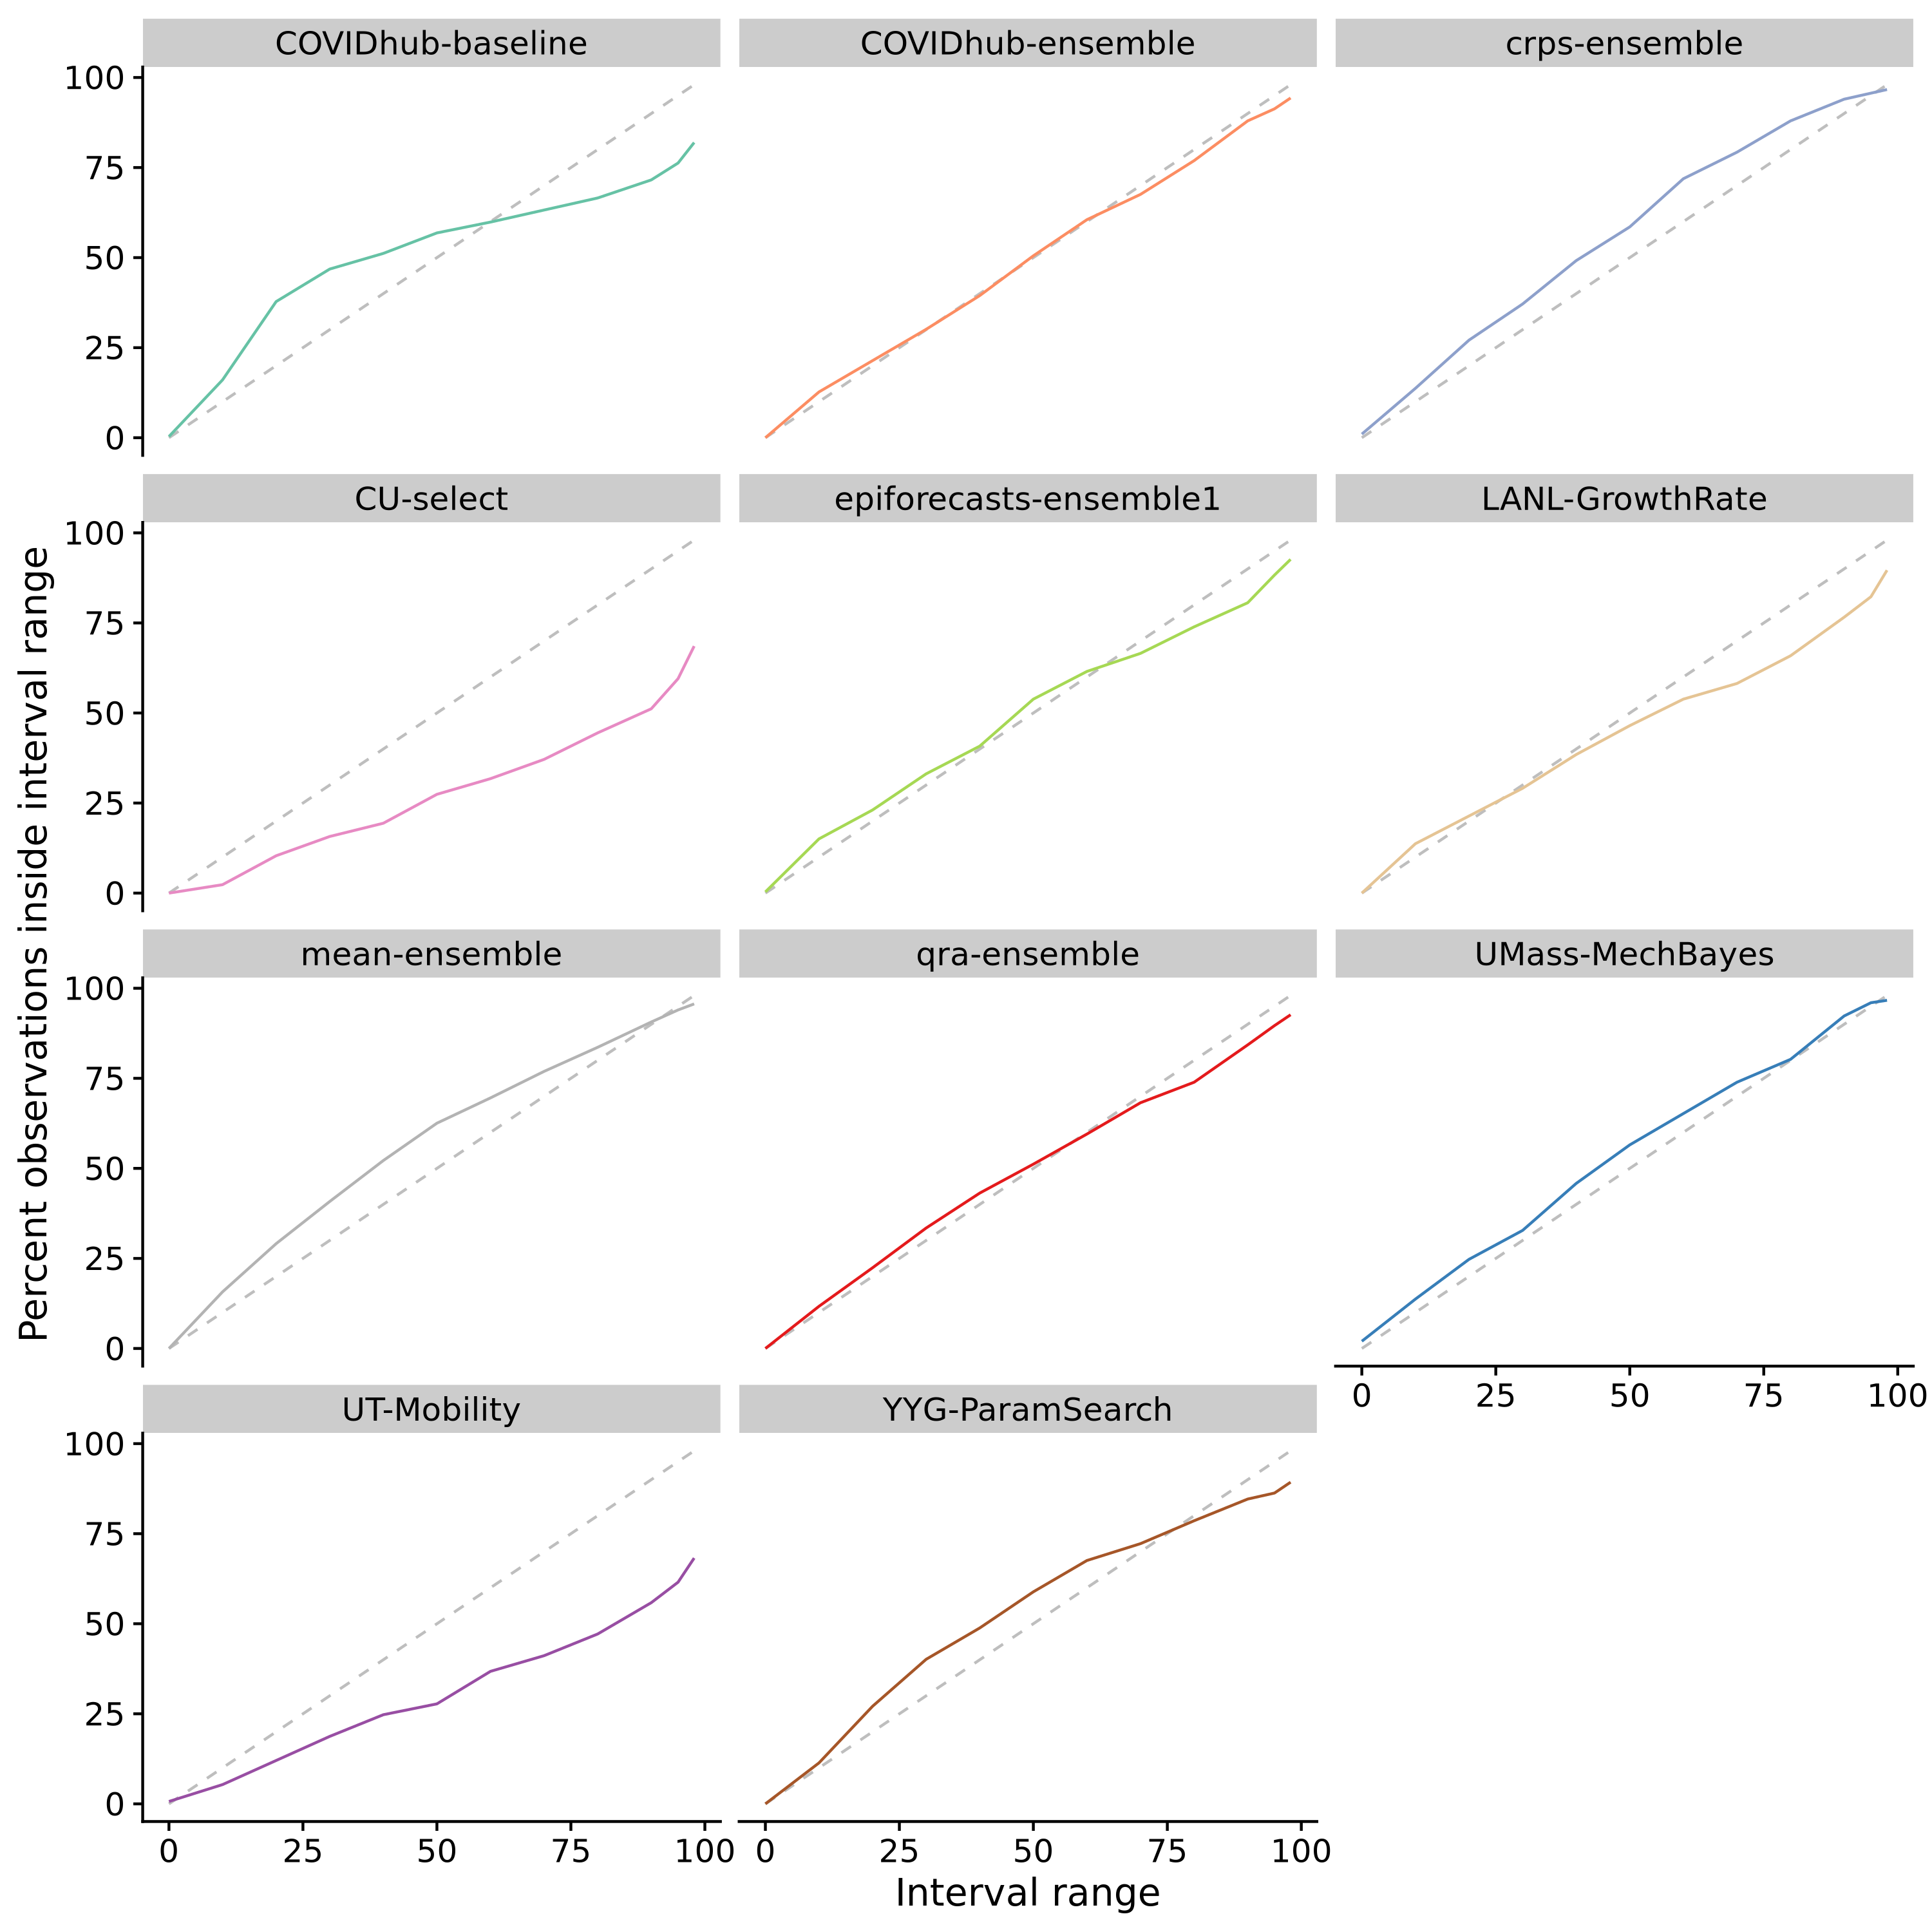
\includegraphics[width=1\linewidth]{../visualisation/chapter-5-results/interval-coverage-all} \caption{Coverage of the prediction intervals across all locations and forecast dates}\label{fig:interval-coverage-all}
\end{figure}

Figure \ref{fig:quantile-coverage-all} therefore goes into more detail and shows quantile coverage, i.e.~the proportion of predictions lower than the true value for each quantile of the model predictions. This makes it possible to see whether a lack of coverage in a certain interval range is more a problem of the lower or the upper bounds of the interval range. For the epiforecasts-ensemble1, for example, we could see a lack of coverage in the outer prediction intervals in Figure \ref{fig:interval-coverage-all}. With the help of the quantile coverage plot we can now see that the problem lies in the upper, rather than the lower bounds. It seems that the epiforecasts-ensemble1 did well in quantifying uncertainty below the median, but was underpredicting the likelihood of extreme events above the median. This quantile coverage visualisation also allows us to reexamine the bias component of calibration again. We can for example see that the UT-Mobility and qra-ensemble, which exhibit an upward bias (compare \ref{fig:coloured-summarised-scores}), are moved to the left of the diagonal, while e.g.~the YYG-ParamSearch or the LANL-GrowthRate model, which are downward biased, are moved to the right.

\begin{figure}
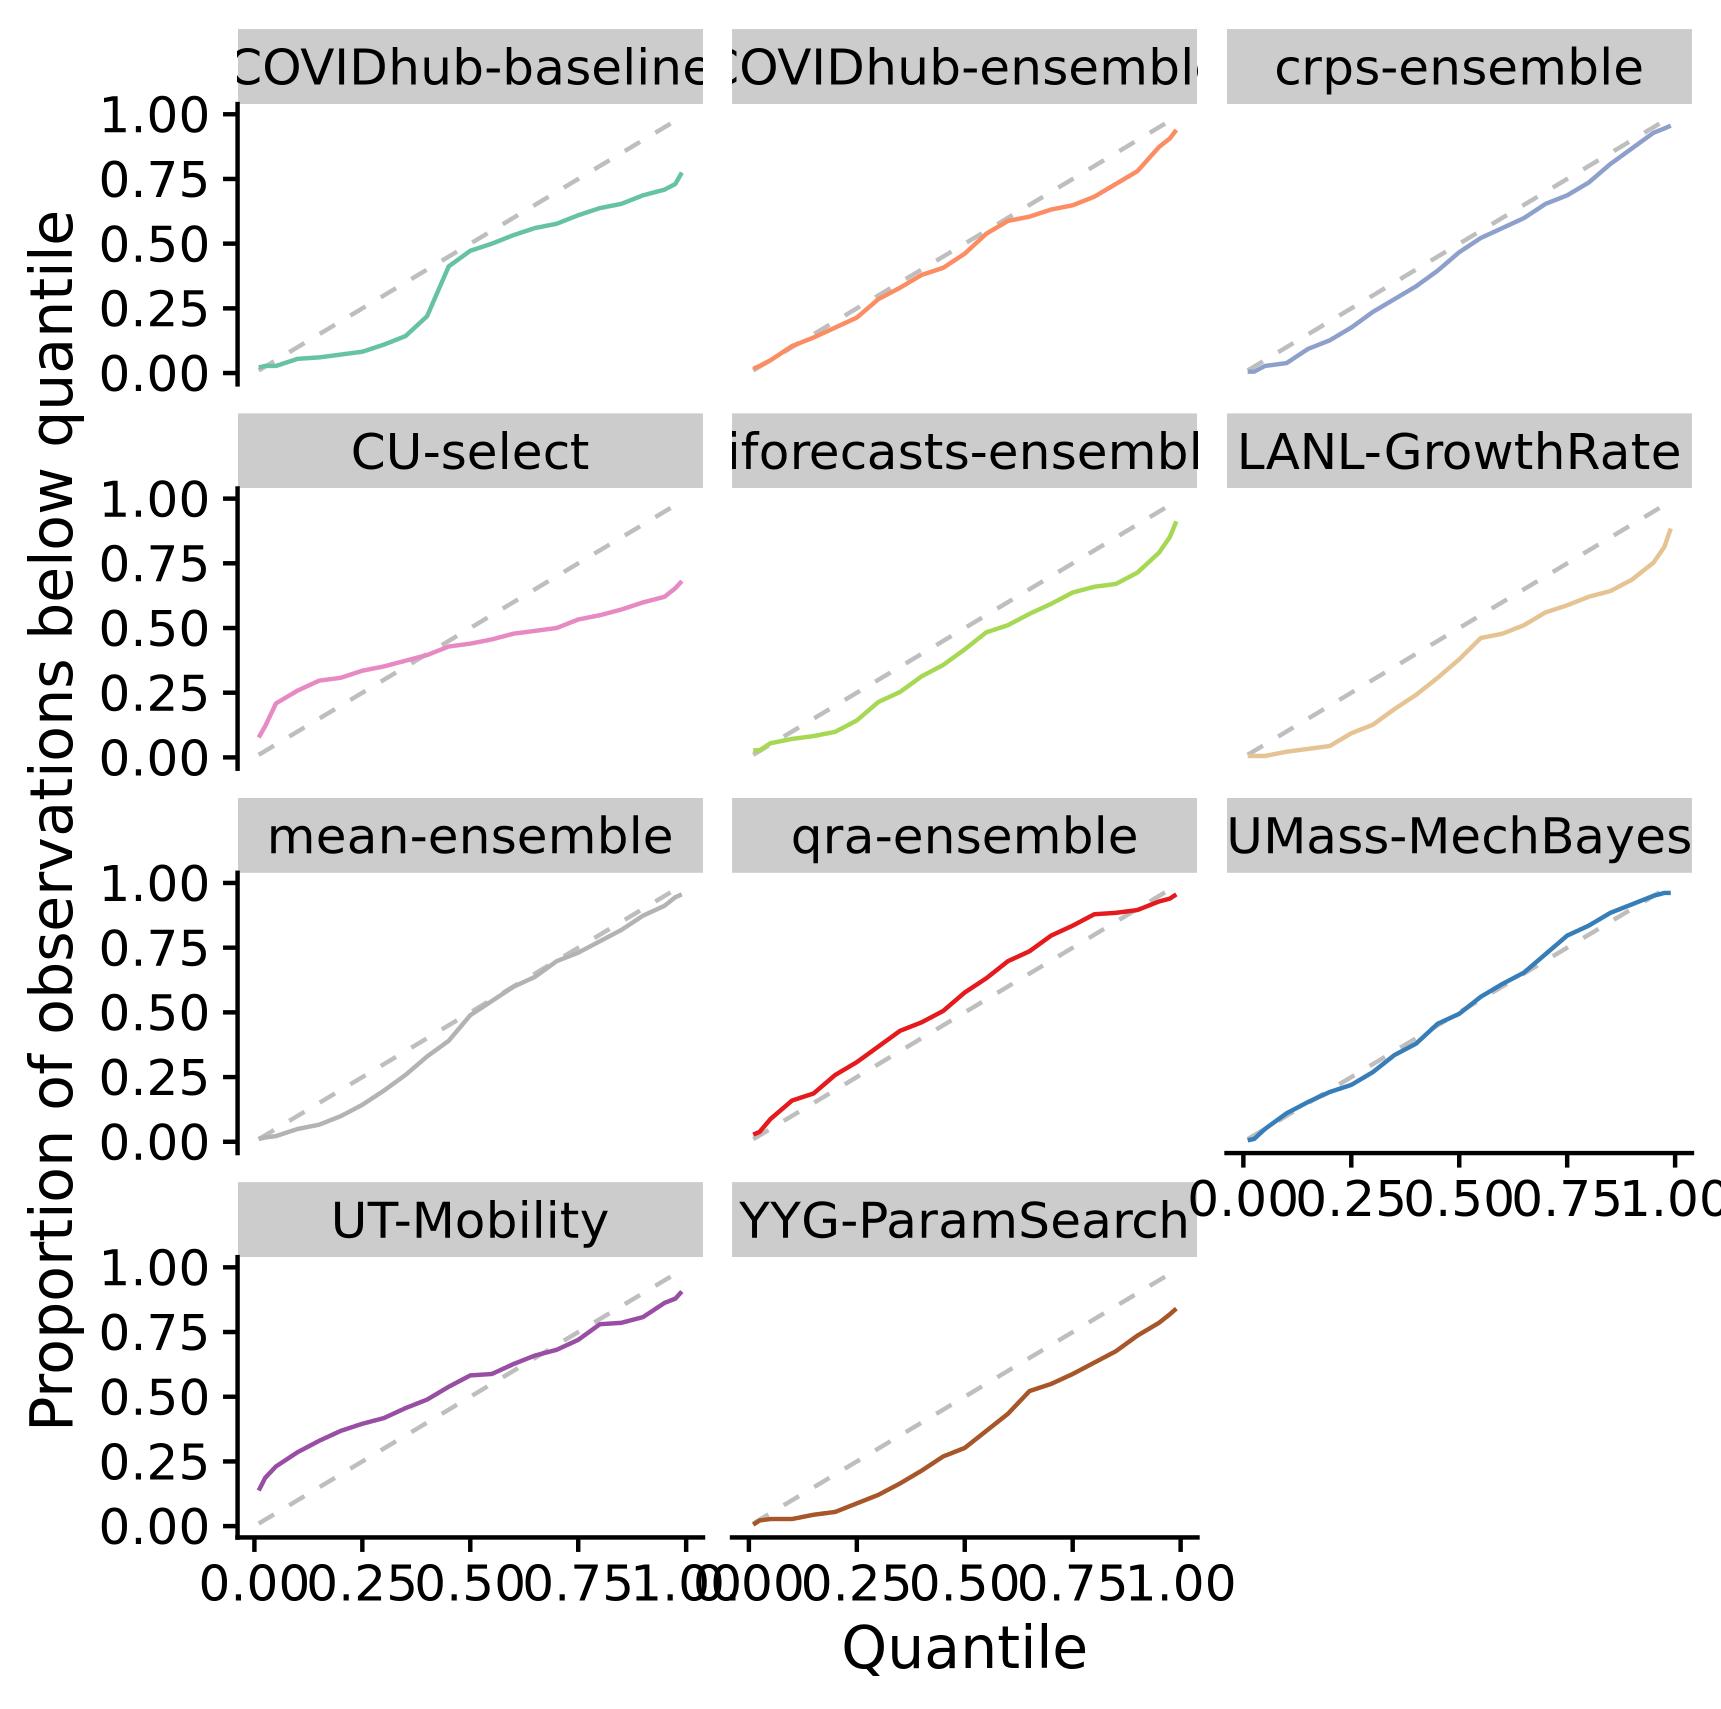
\includegraphics[width=1\linewidth]{../visualisation/chapter-5-results/quantile-coverage-all} \caption{Coverage of the prediction intervals across all locations and forecast dates}\label{fig:quantile-coverage-all}
\end{figure}

One major advantage this type of visualisation has over PIT histograms is that we can easily compare different models in a single plot. Figure \ref{fig:coverage-ensemble} exemplifies this for the ensemble models. It is obvious taht the COVIDhub-ensemble did best in terms of interval as well as quantile coverage. The crps-ensemble and the mean-ensemble have a slightly too high interval coverage, which we confirms what we have already seen in the summarised scores in Figure \ref{fig:coloured-summarised-scores}. Looking at the quantile coverage plot (on the right) we can see clearly see that the qra-ensemble model is the most biased of all ensemble models. It is therefore maybe surprising to see the model looks quite well in terms of interval coverage (on the left). We can explain this discrepancy by taking sharpness into account. In Figure \ref{fig:coloured-summarised-scores} we could see that the COVIDhub-ensemble was much sharper than the other three ensembles which were about equally sharp. For the mean-ensemble and the crps-ensemble the increased width of the prediction intervals for the translated into a positive coverage deviation, while for the qra-ensemble it only mitigated the effect the increased bias would have had on interval coverage. This discrepancy between quantile and interval coverage, however, highlights again that interval coverage only shows one kind of calibration. Good interval coverage is a necessary condition, but not sufficient to prove good calibration. In general, it seems that the quantile plot (right) visually correlates better with overall model performance as judged by WIS. We should therefore look at the quantile coverage plot rather than the interval coverage plot if we were to choose only one.

\begin{figure}
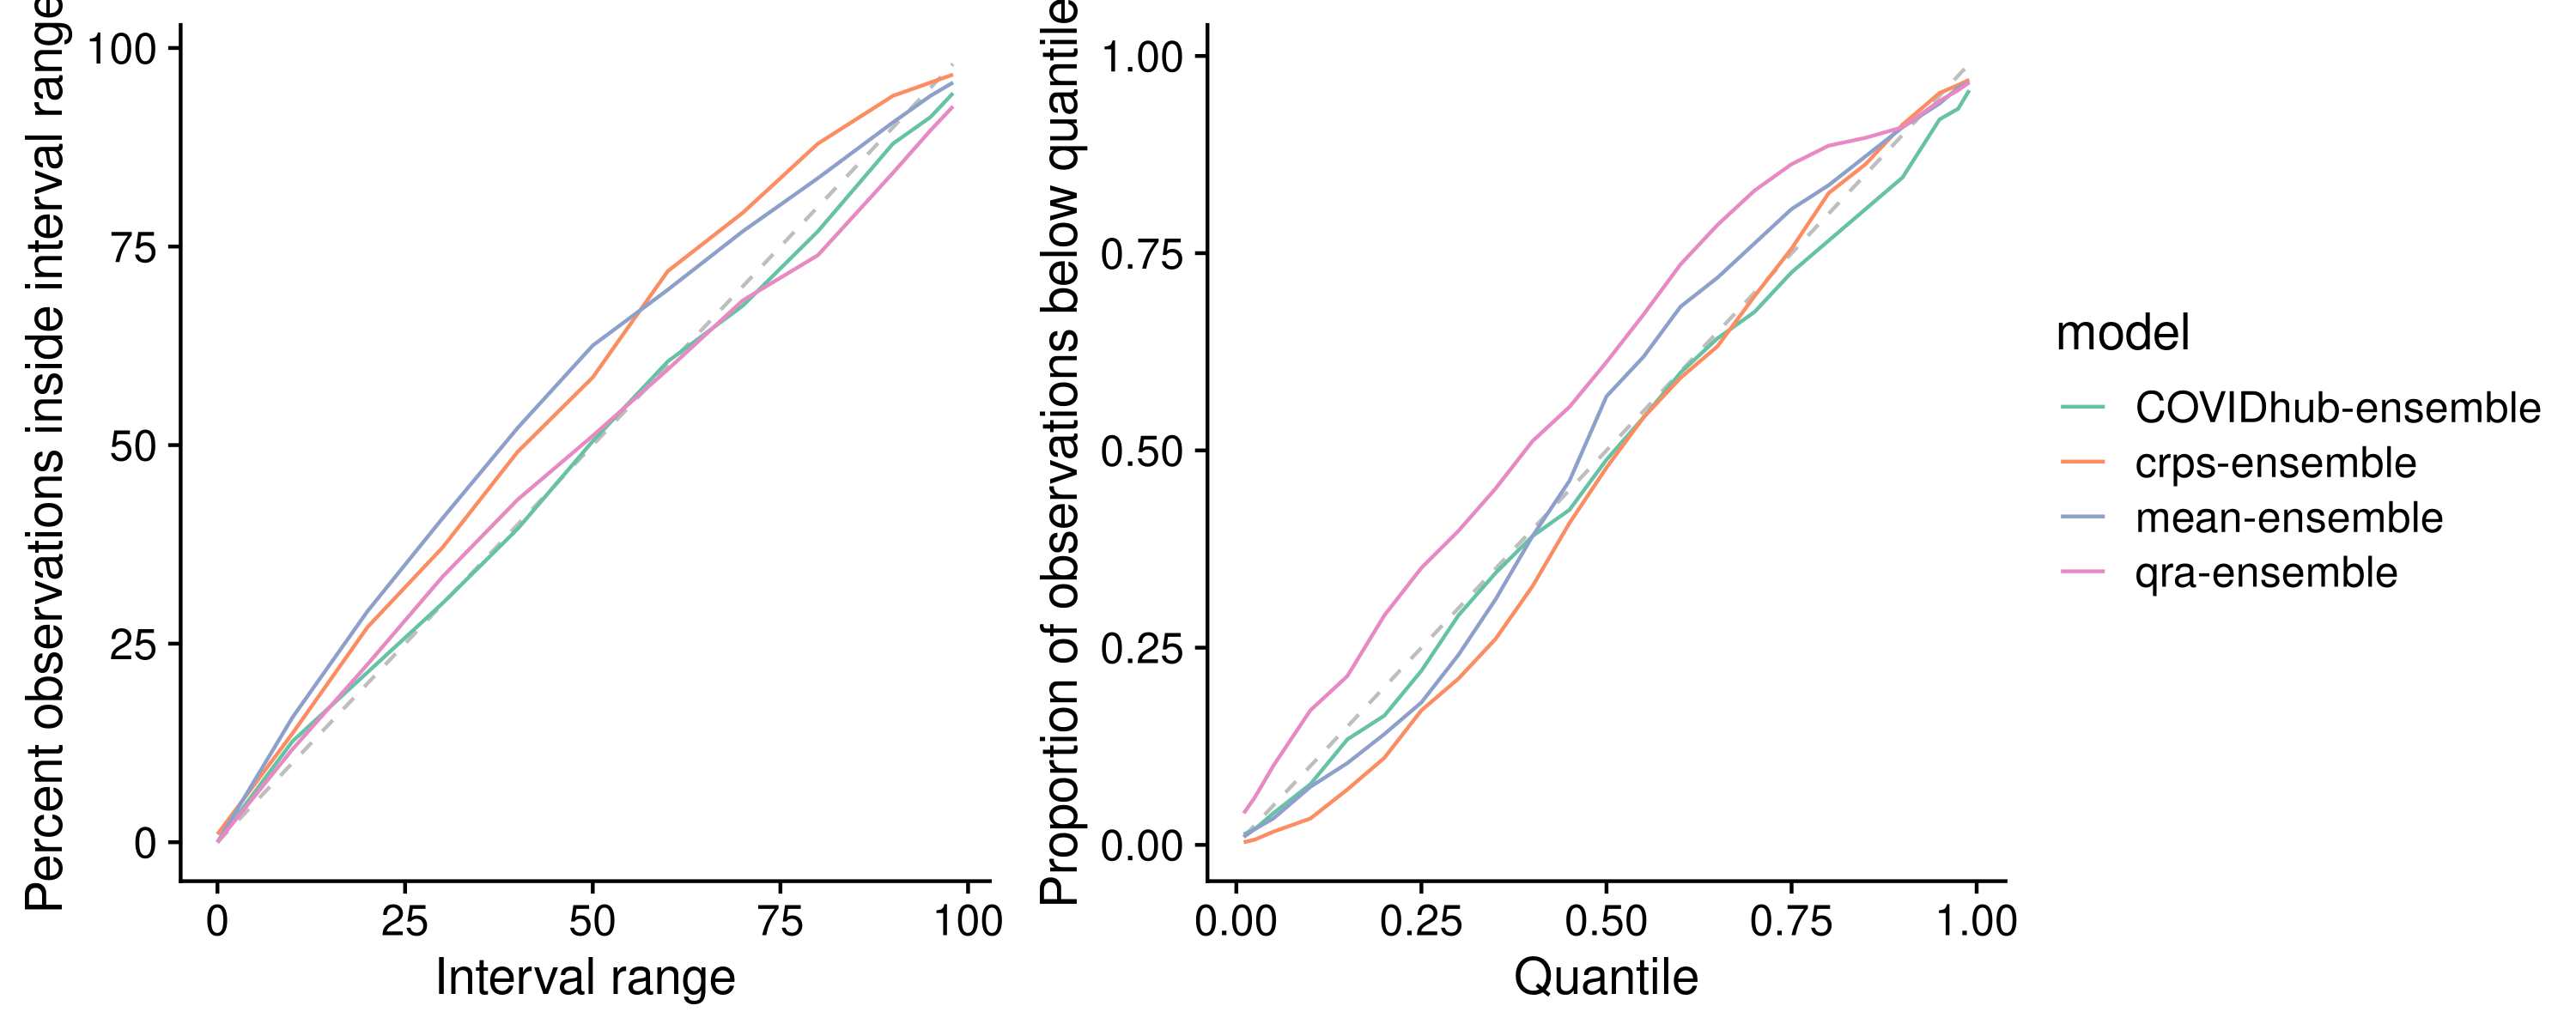
\includegraphics[width=1\linewidth]{../visualisation/chapter-5-results/coverage_ensemble} \caption{Interval coverage (left) and quantile coverage (right)}\label{fig:coverage-ensemble}
\end{figure}

\hypertarget{coverage-by-subgroups}{%
\subsubsection{Coverage by subgroups}\label{coverage-by-subgroups}}

We can again look at coverage in different subgroups to get a better understanding for how the models and the metrics behave. We might for example want to ask how coverage changes over different prediction horizons, as this could give an indication of how well we far into the future we can confidently make predictions. Figures \ref{fig:interval-coverage-horizon} and \ref{fig:quantile-coverage-horizon} show the interval and quantile coverage over different prediction horizons. We can generally see that coverage generally tends to deteriorate at least slightly with increasing forecast horizons for many models. WORK ON THIS INTERPRETATION OR MAYBE JUST MOVE THE PLOTS TO THE APPENDIX.

\begin{figure}
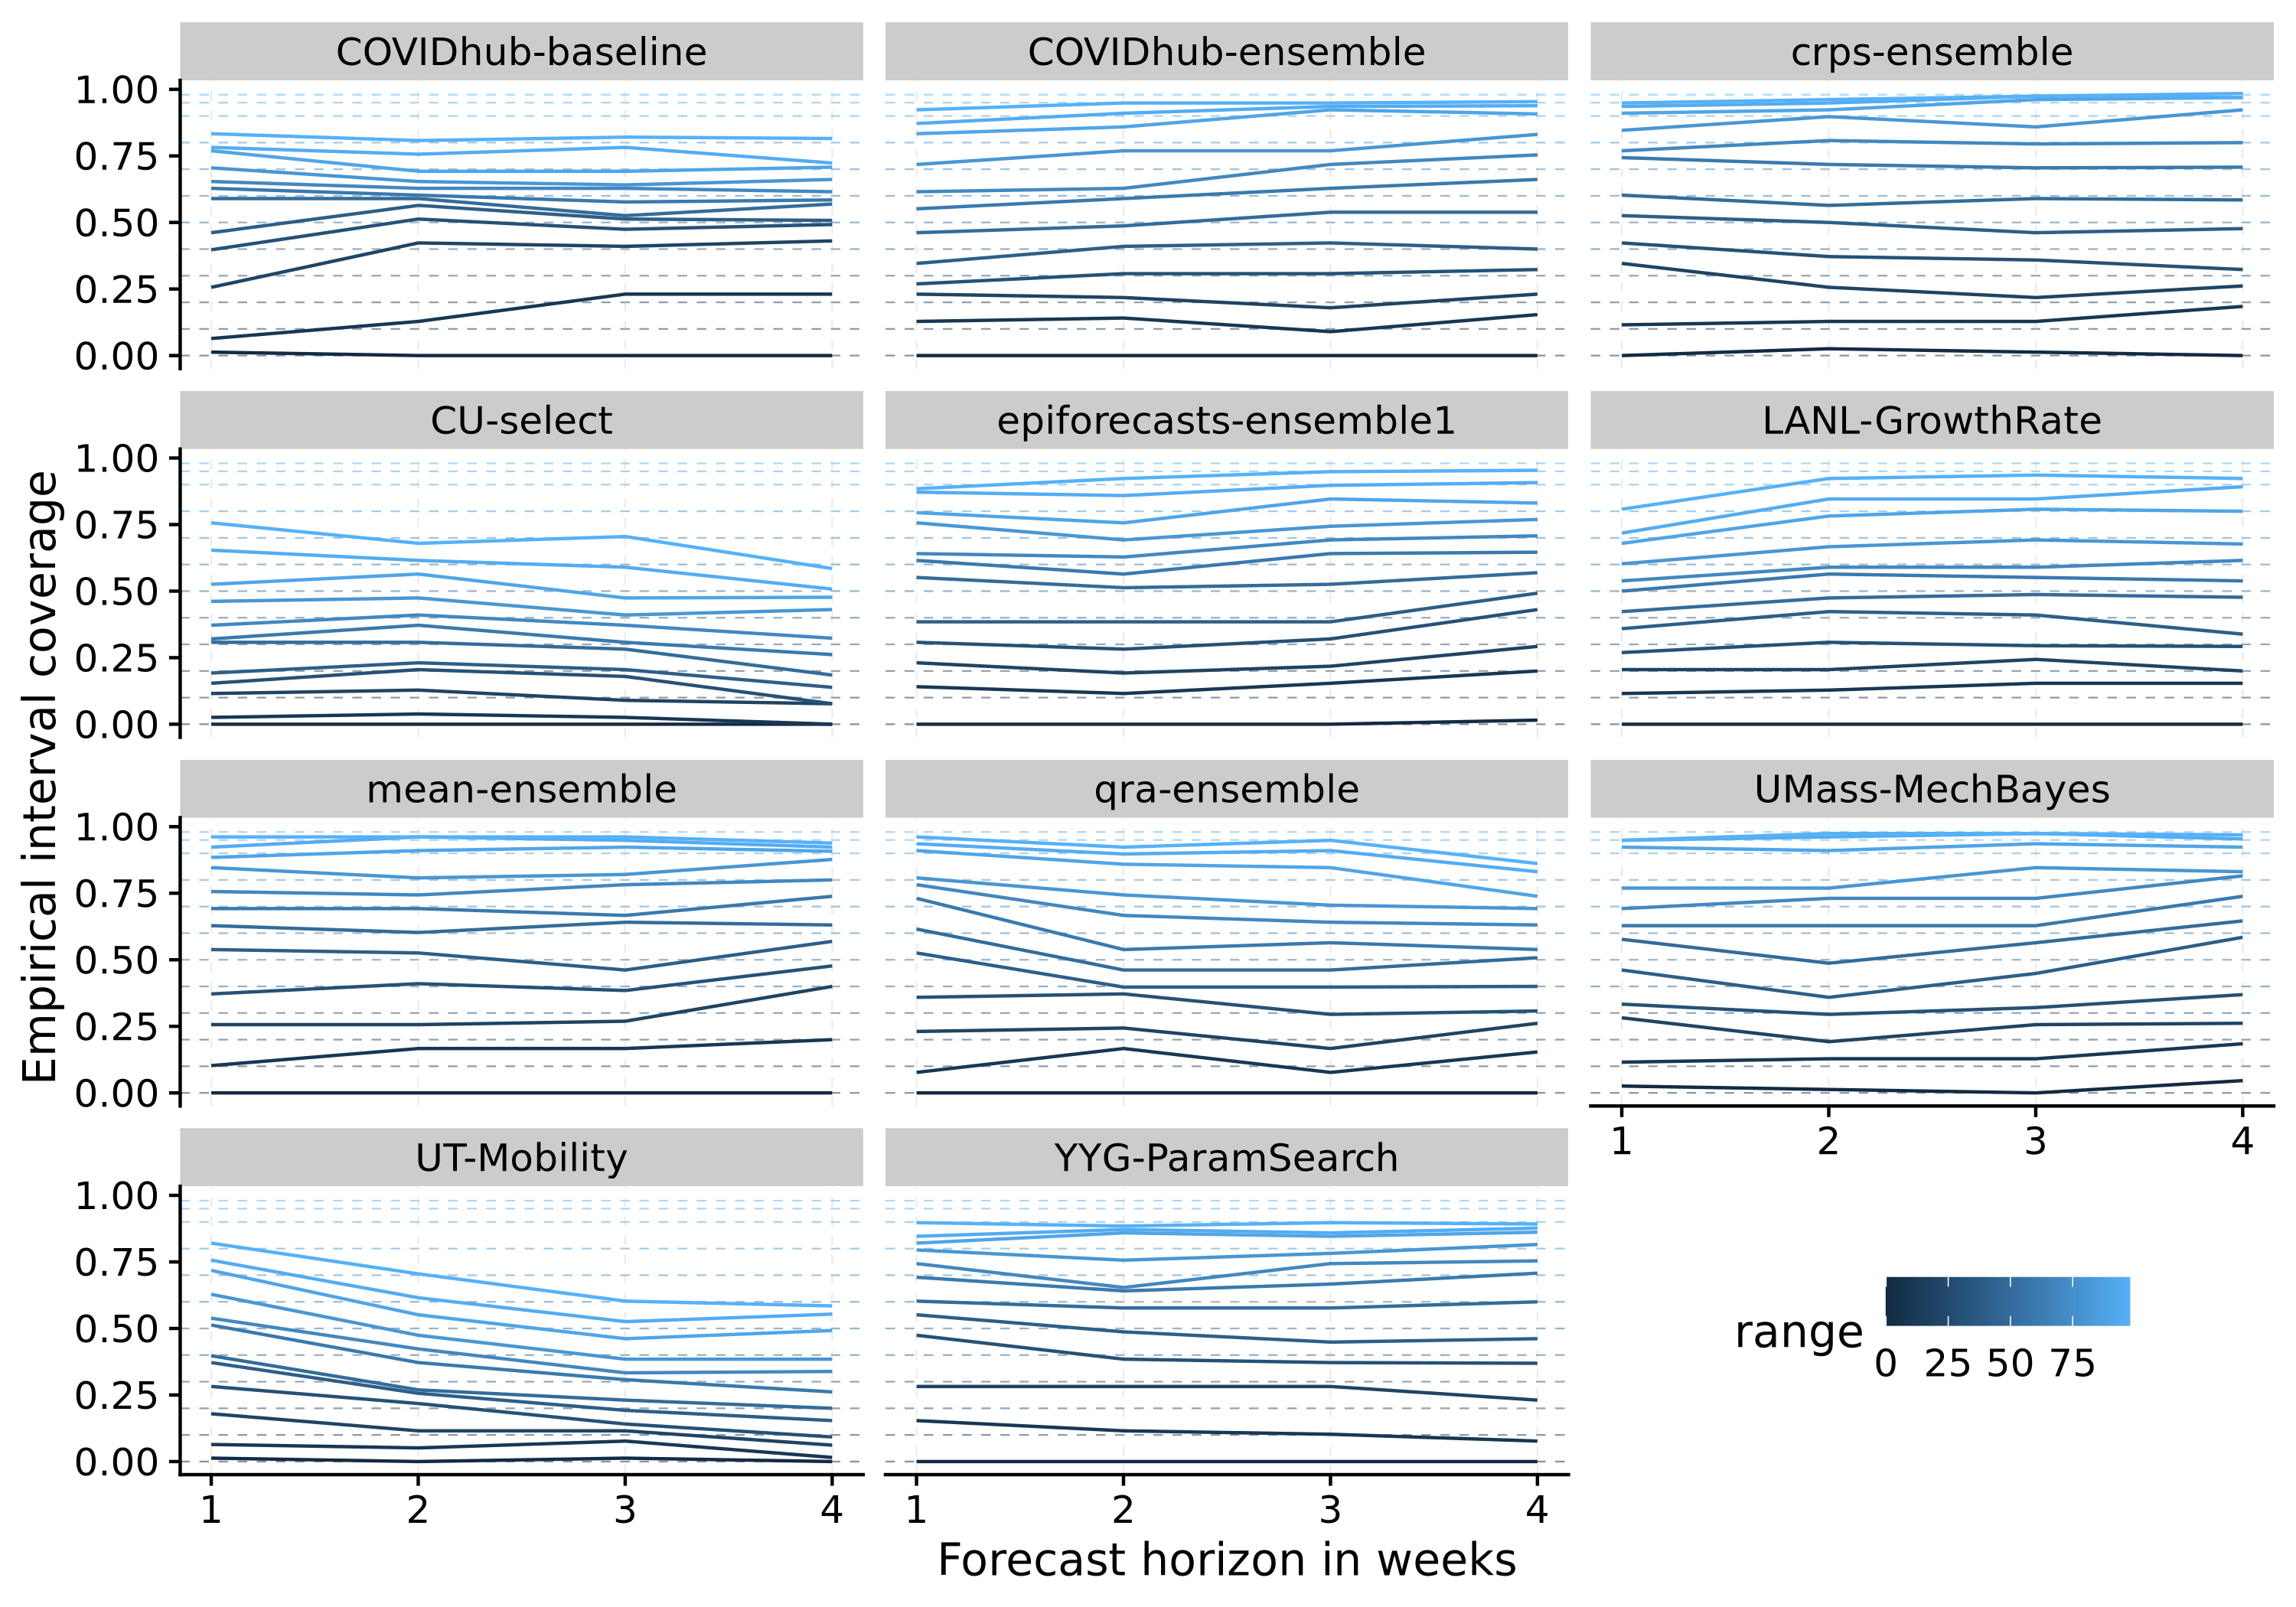
\includegraphics[width=1\linewidth]{../visualisation/chapter-5-results/interval-coverage-horizons} \caption{Coverage of the prediction intervals across all locations and forecast dates over different horizons}\label{fig:interval-coverage-horizon}
\end{figure}

\begin{figure}
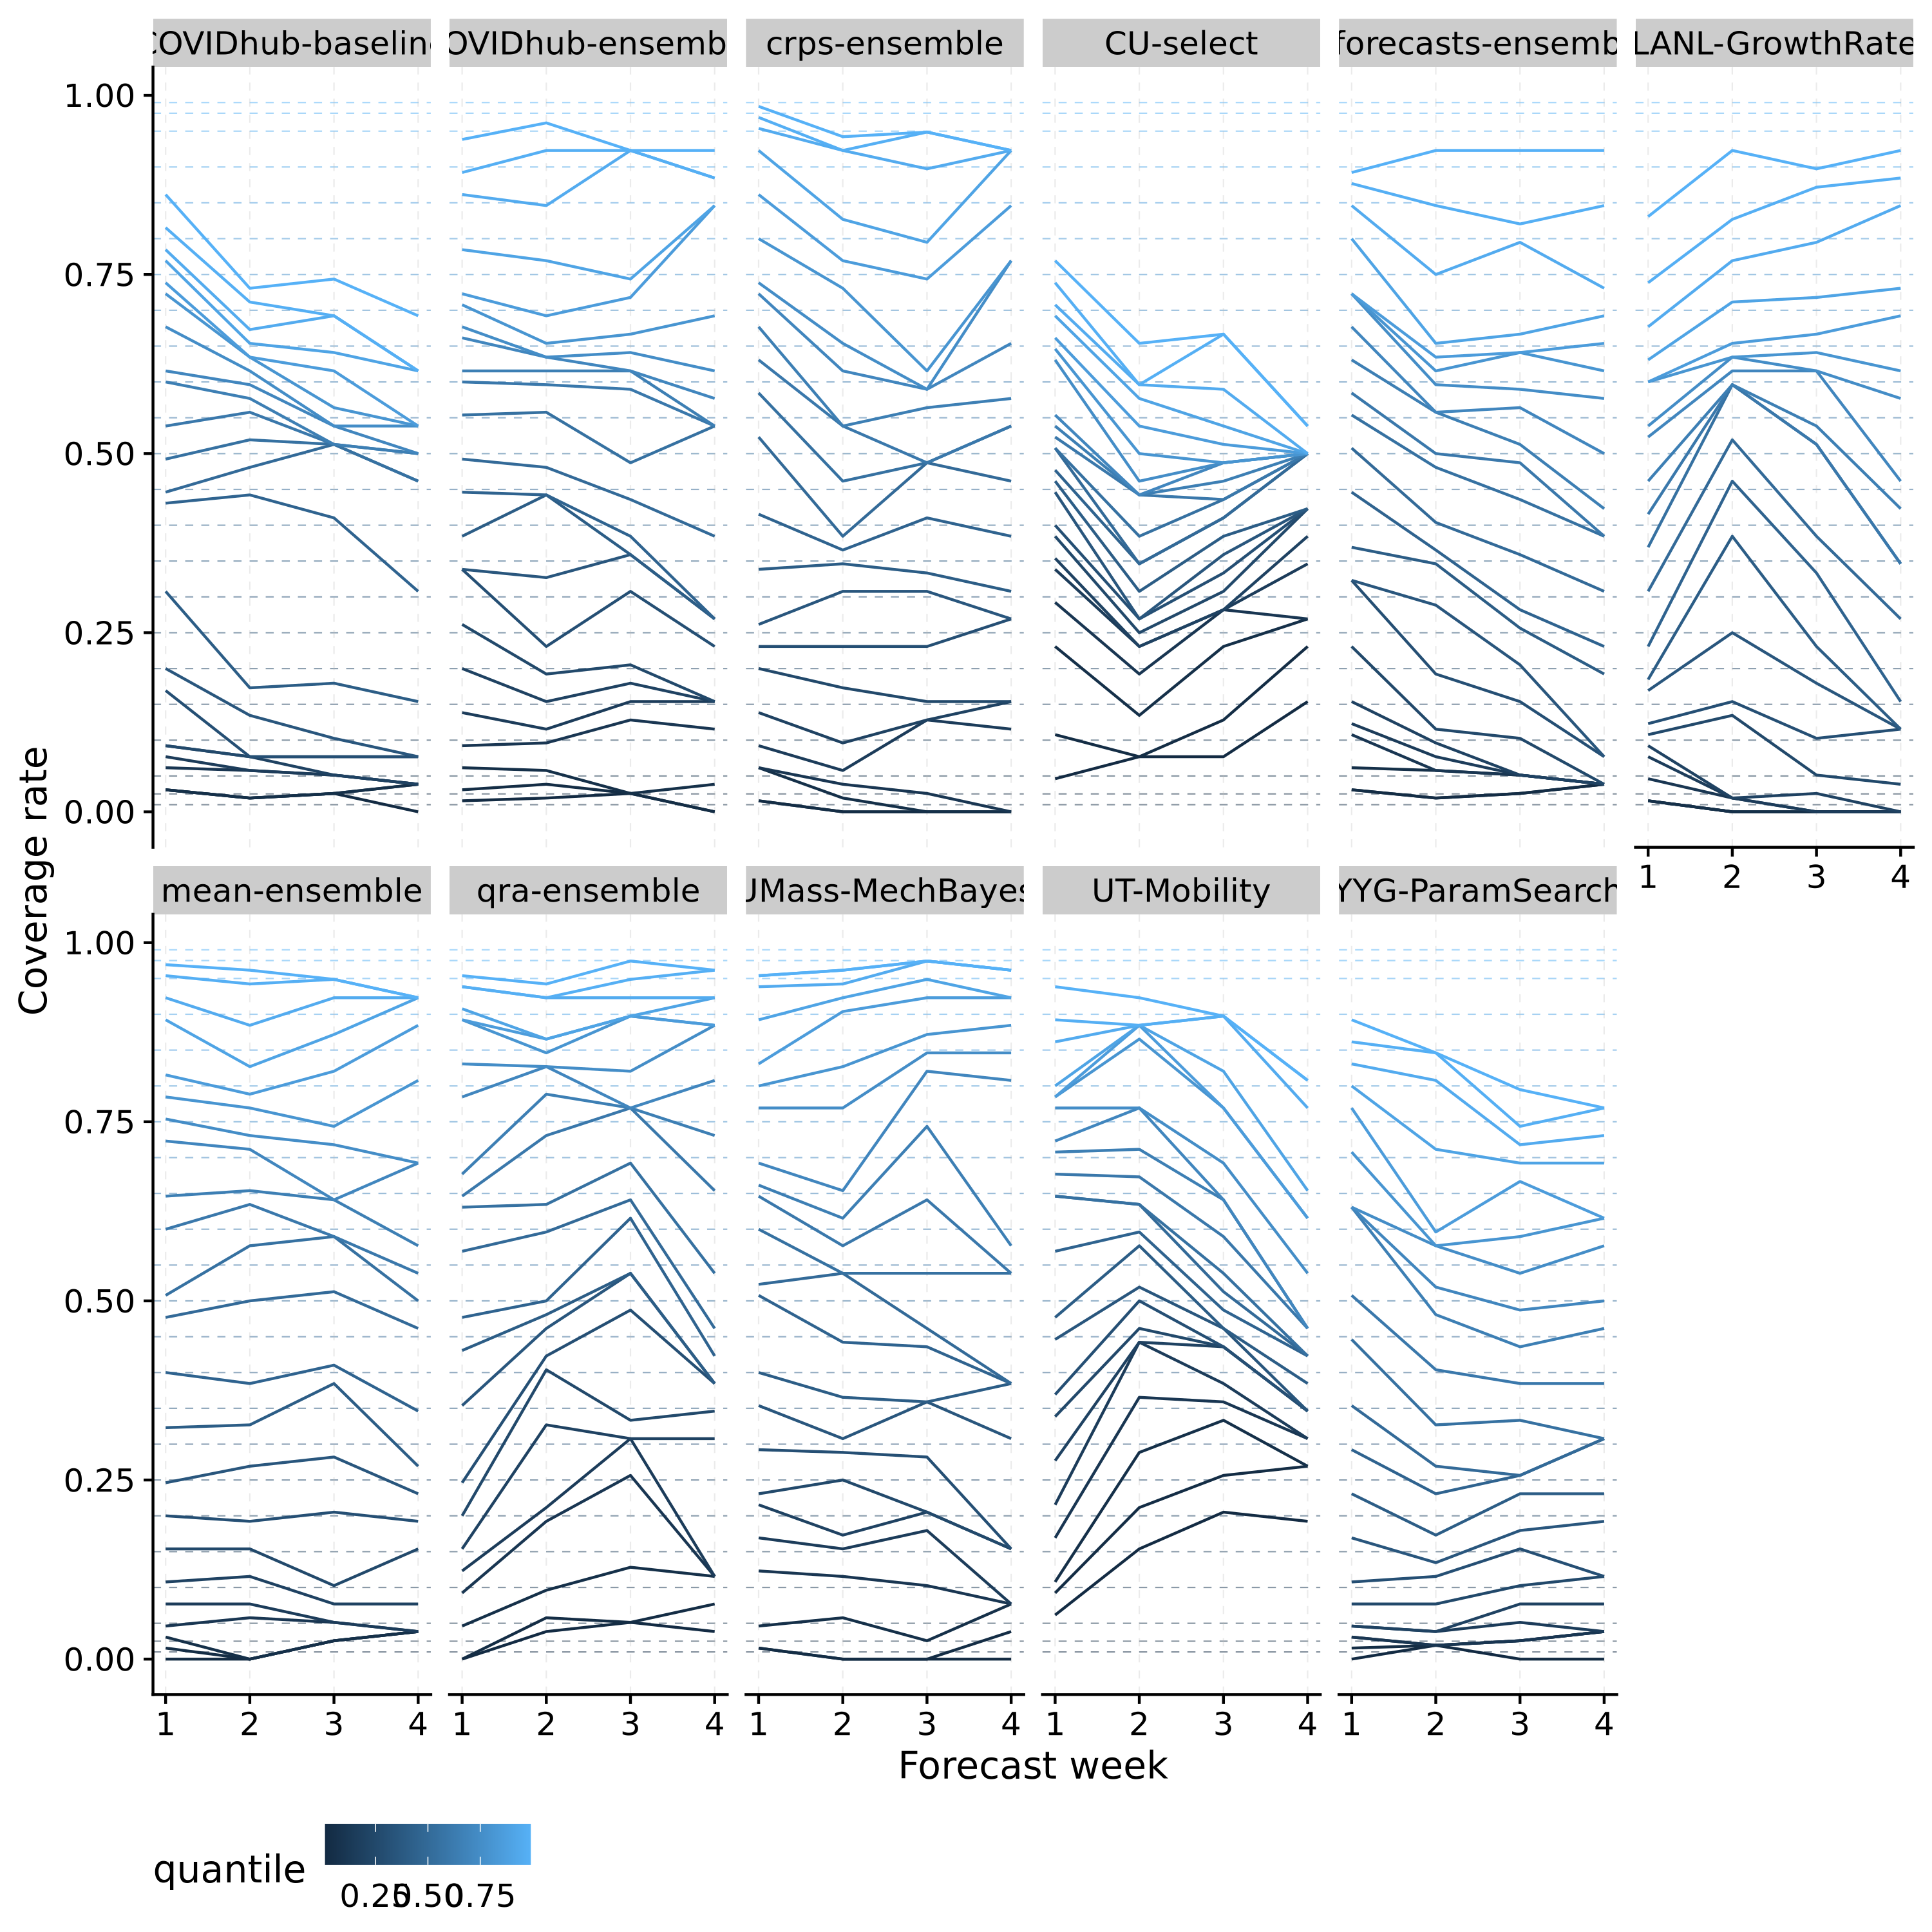
\includegraphics[width=1\linewidth]{../visualisation/chapter-5-results/quantile-coverage-horizons} \caption{Coverage of the prediction intervals across all locations and forecast dates over different horizons}\label{fig:quantile-coverage-horizon}
\end{figure}

As before, we may also be interested in how different ranges contribute to overall coverage deviation. \ref{fig:coverage-deviation-range} therefore shows coverage deviation by range. MAYBE THIS PLOT IS NOT SO INTERESTING AND I SHOULD DROP IT. A MAYBE MORE INTERSTING PLOT COULD BE COVERAGE DEVIATION BY QUANTILE - THIS WOULD GIVE A MAYBE NICE VISUALISATION OF BIAS.

\begin{figure}
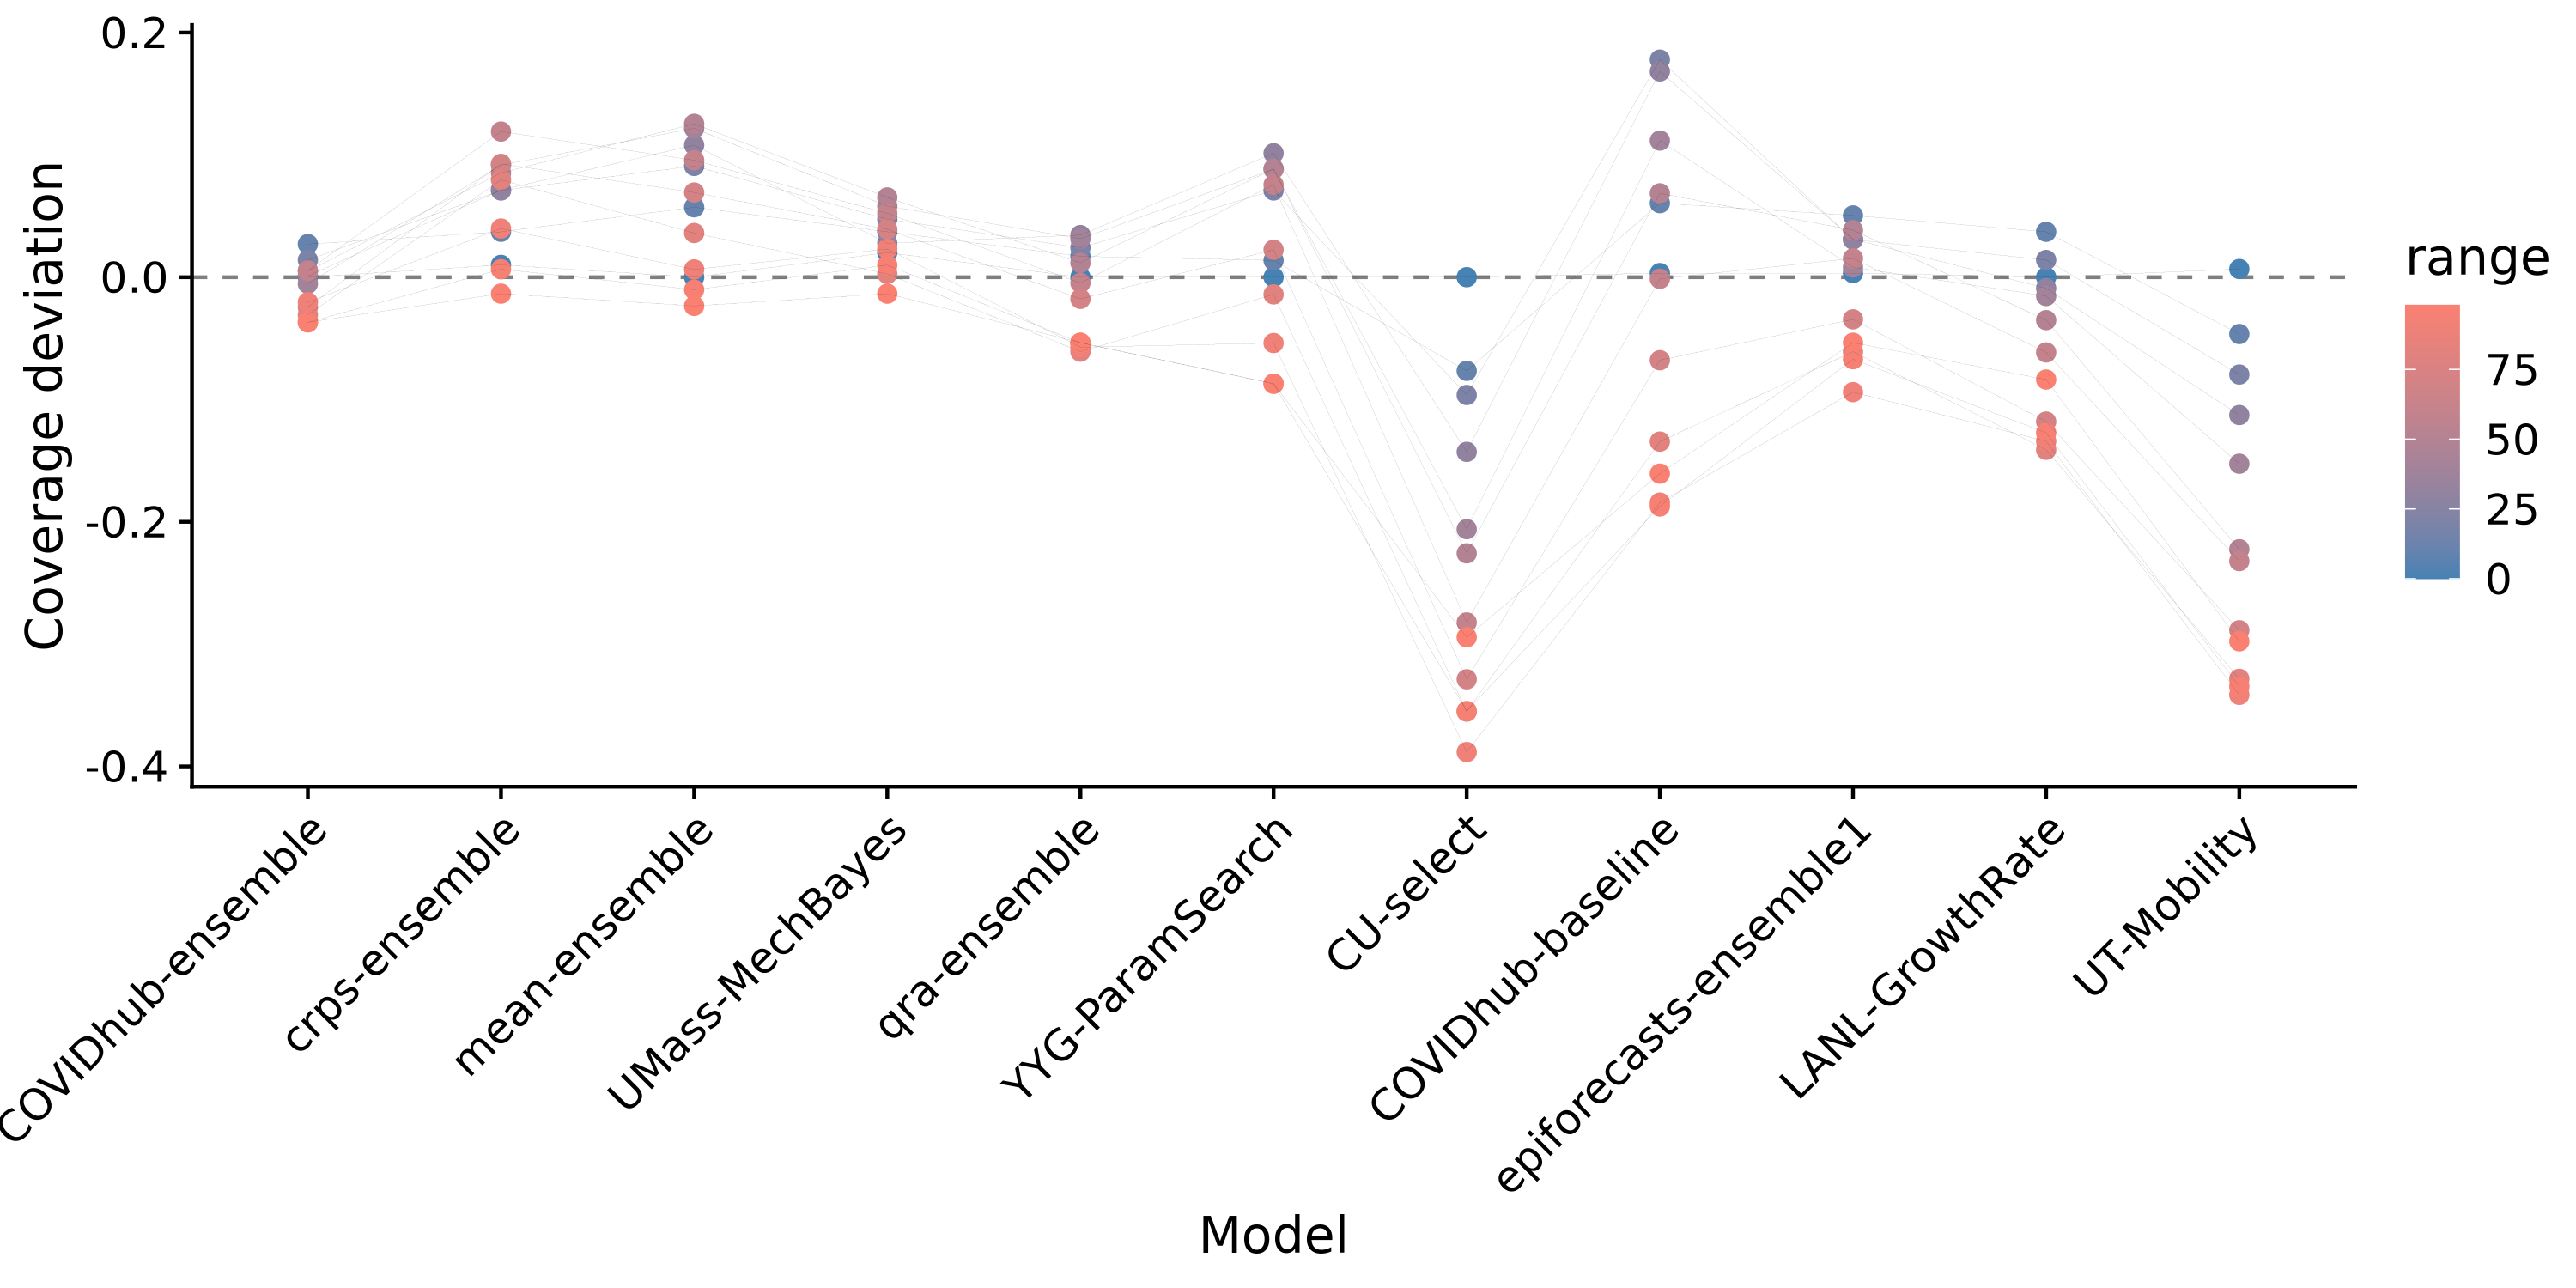
\includegraphics[width=1\linewidth]{../visualisation/chapter-5-results/coverage-deviation-by-range} \caption{Coverage deviation for different ranges}\label{fig:coverage-deviation-range}
\end{figure}

Coverage deviation by state is interesting as it gives us some feeling for how hard different states are to forecast. Figure \ref{fig:coverage-deviation-states} shows the deviation by state. We see that some states are very prone to over- and underprediction. While better performing models tend to be more right we see that all models fail significantly in states like Texas. Figure \ref{fig:pred-texas} shows one-week-ahead predictions and observed values in Texas. Surprisingly, all models are unable to keep up with the change in trend.

\begin{figure}
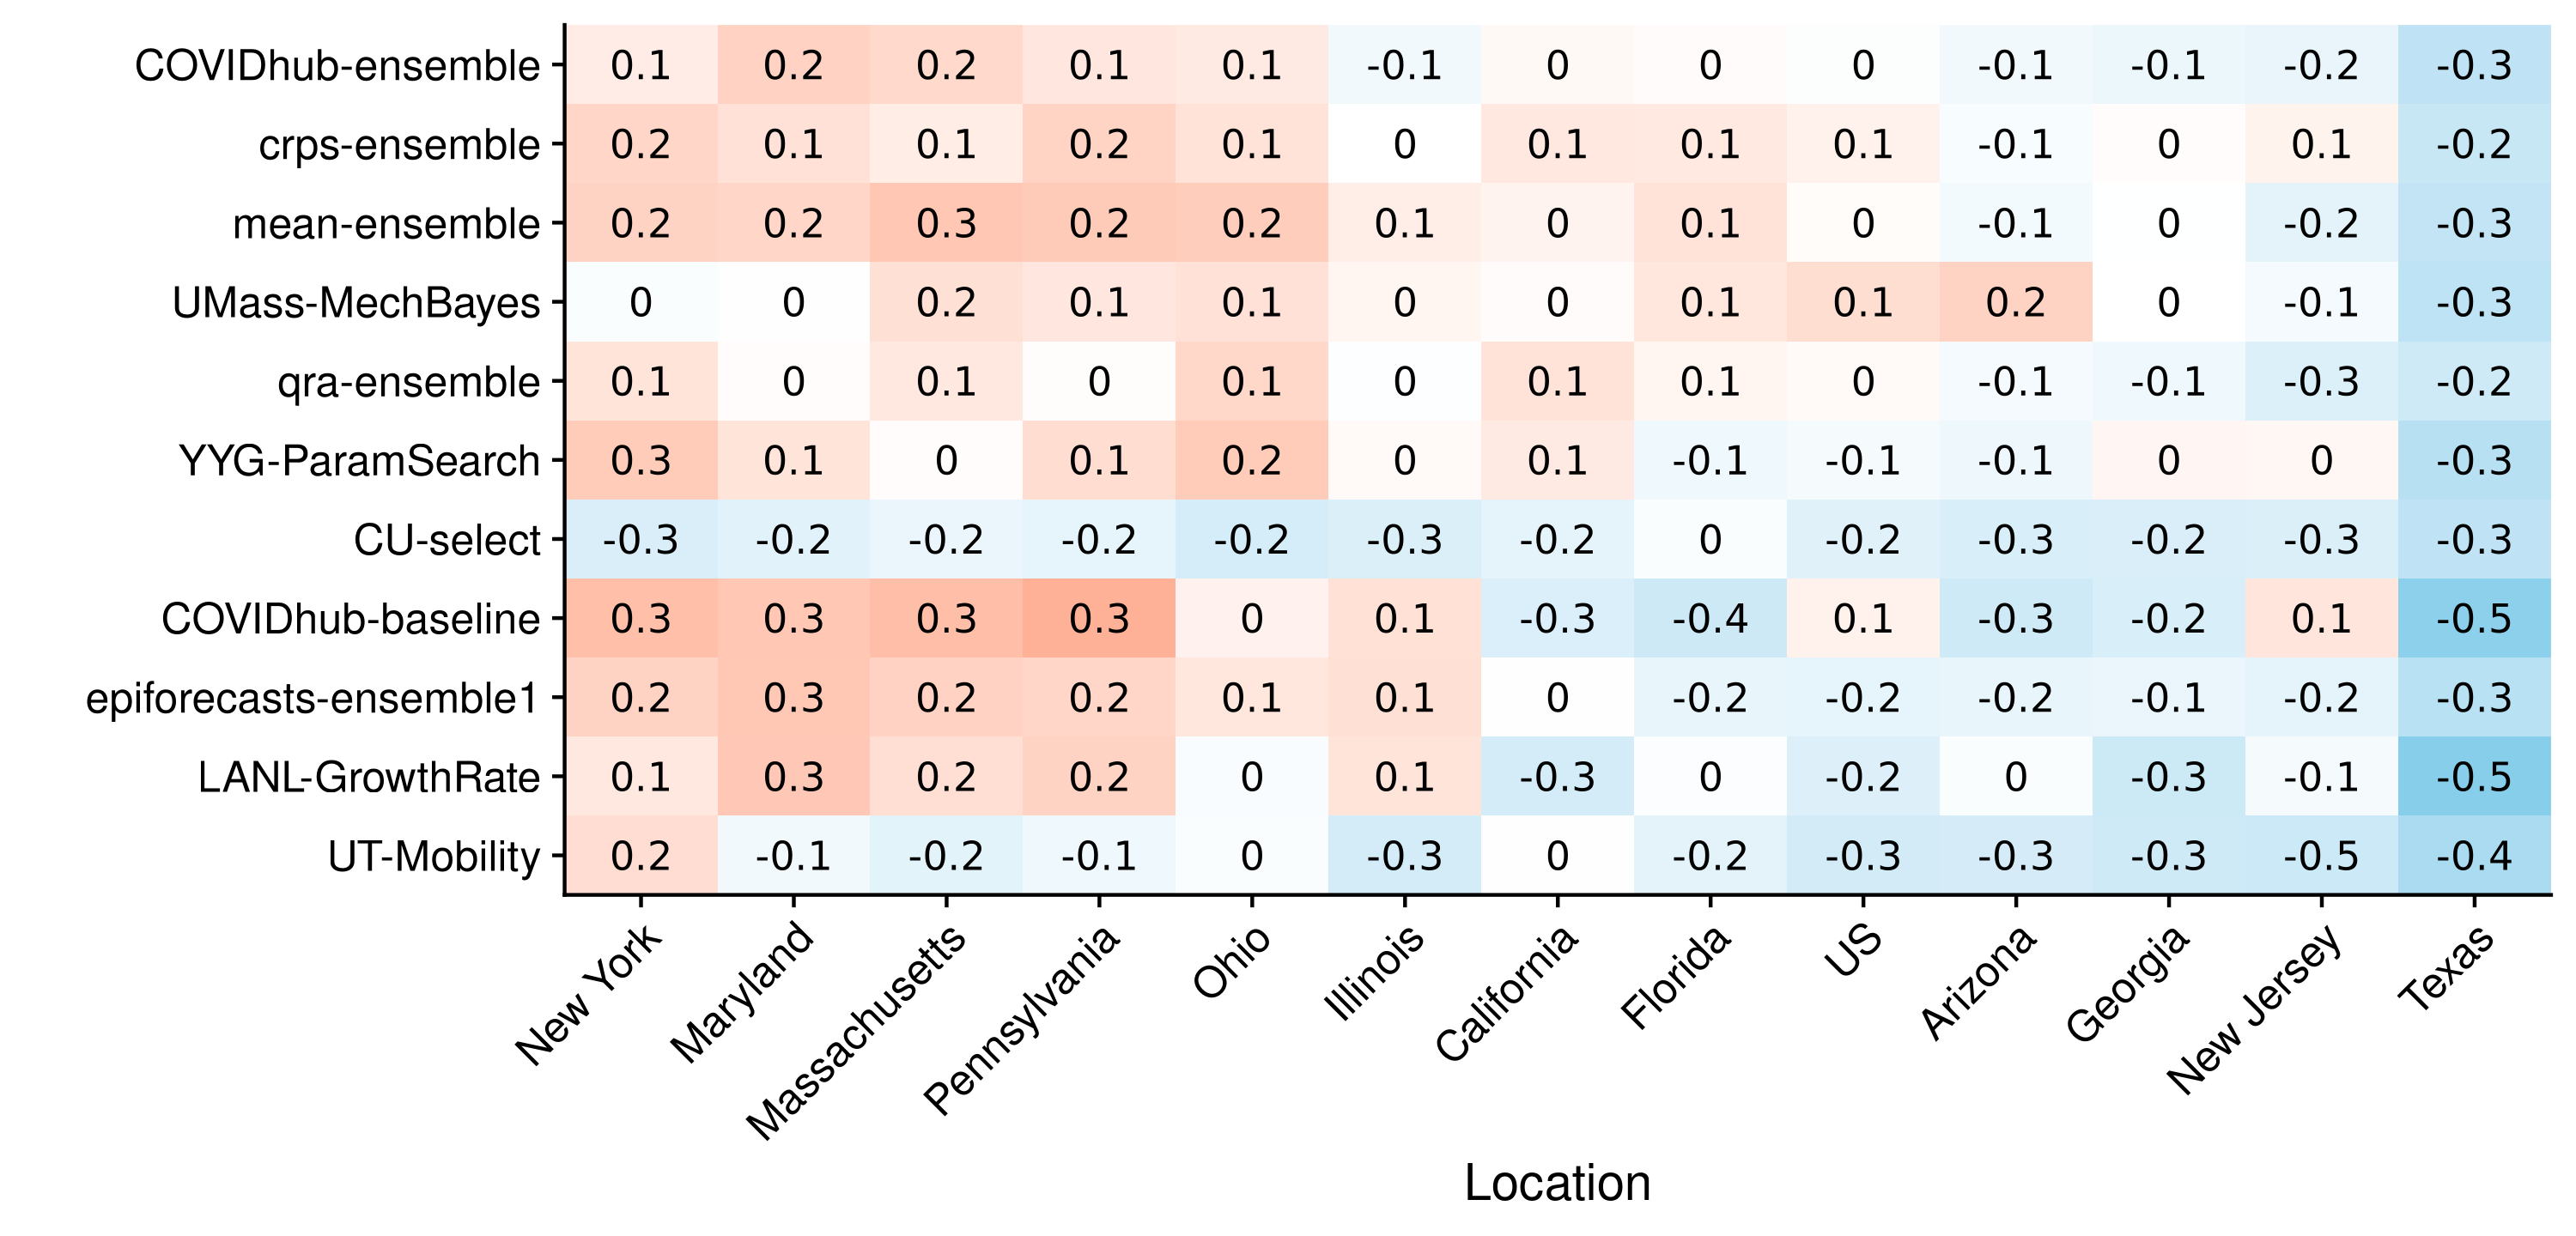
\includegraphics[width=1\linewidth]{../visualisation/chapter-5-results/heatmap-model-coverage} \caption{Coverage deviation for different ranges}\label{fig:coverage-deviation-states}
\end{figure}
\begin{figure}
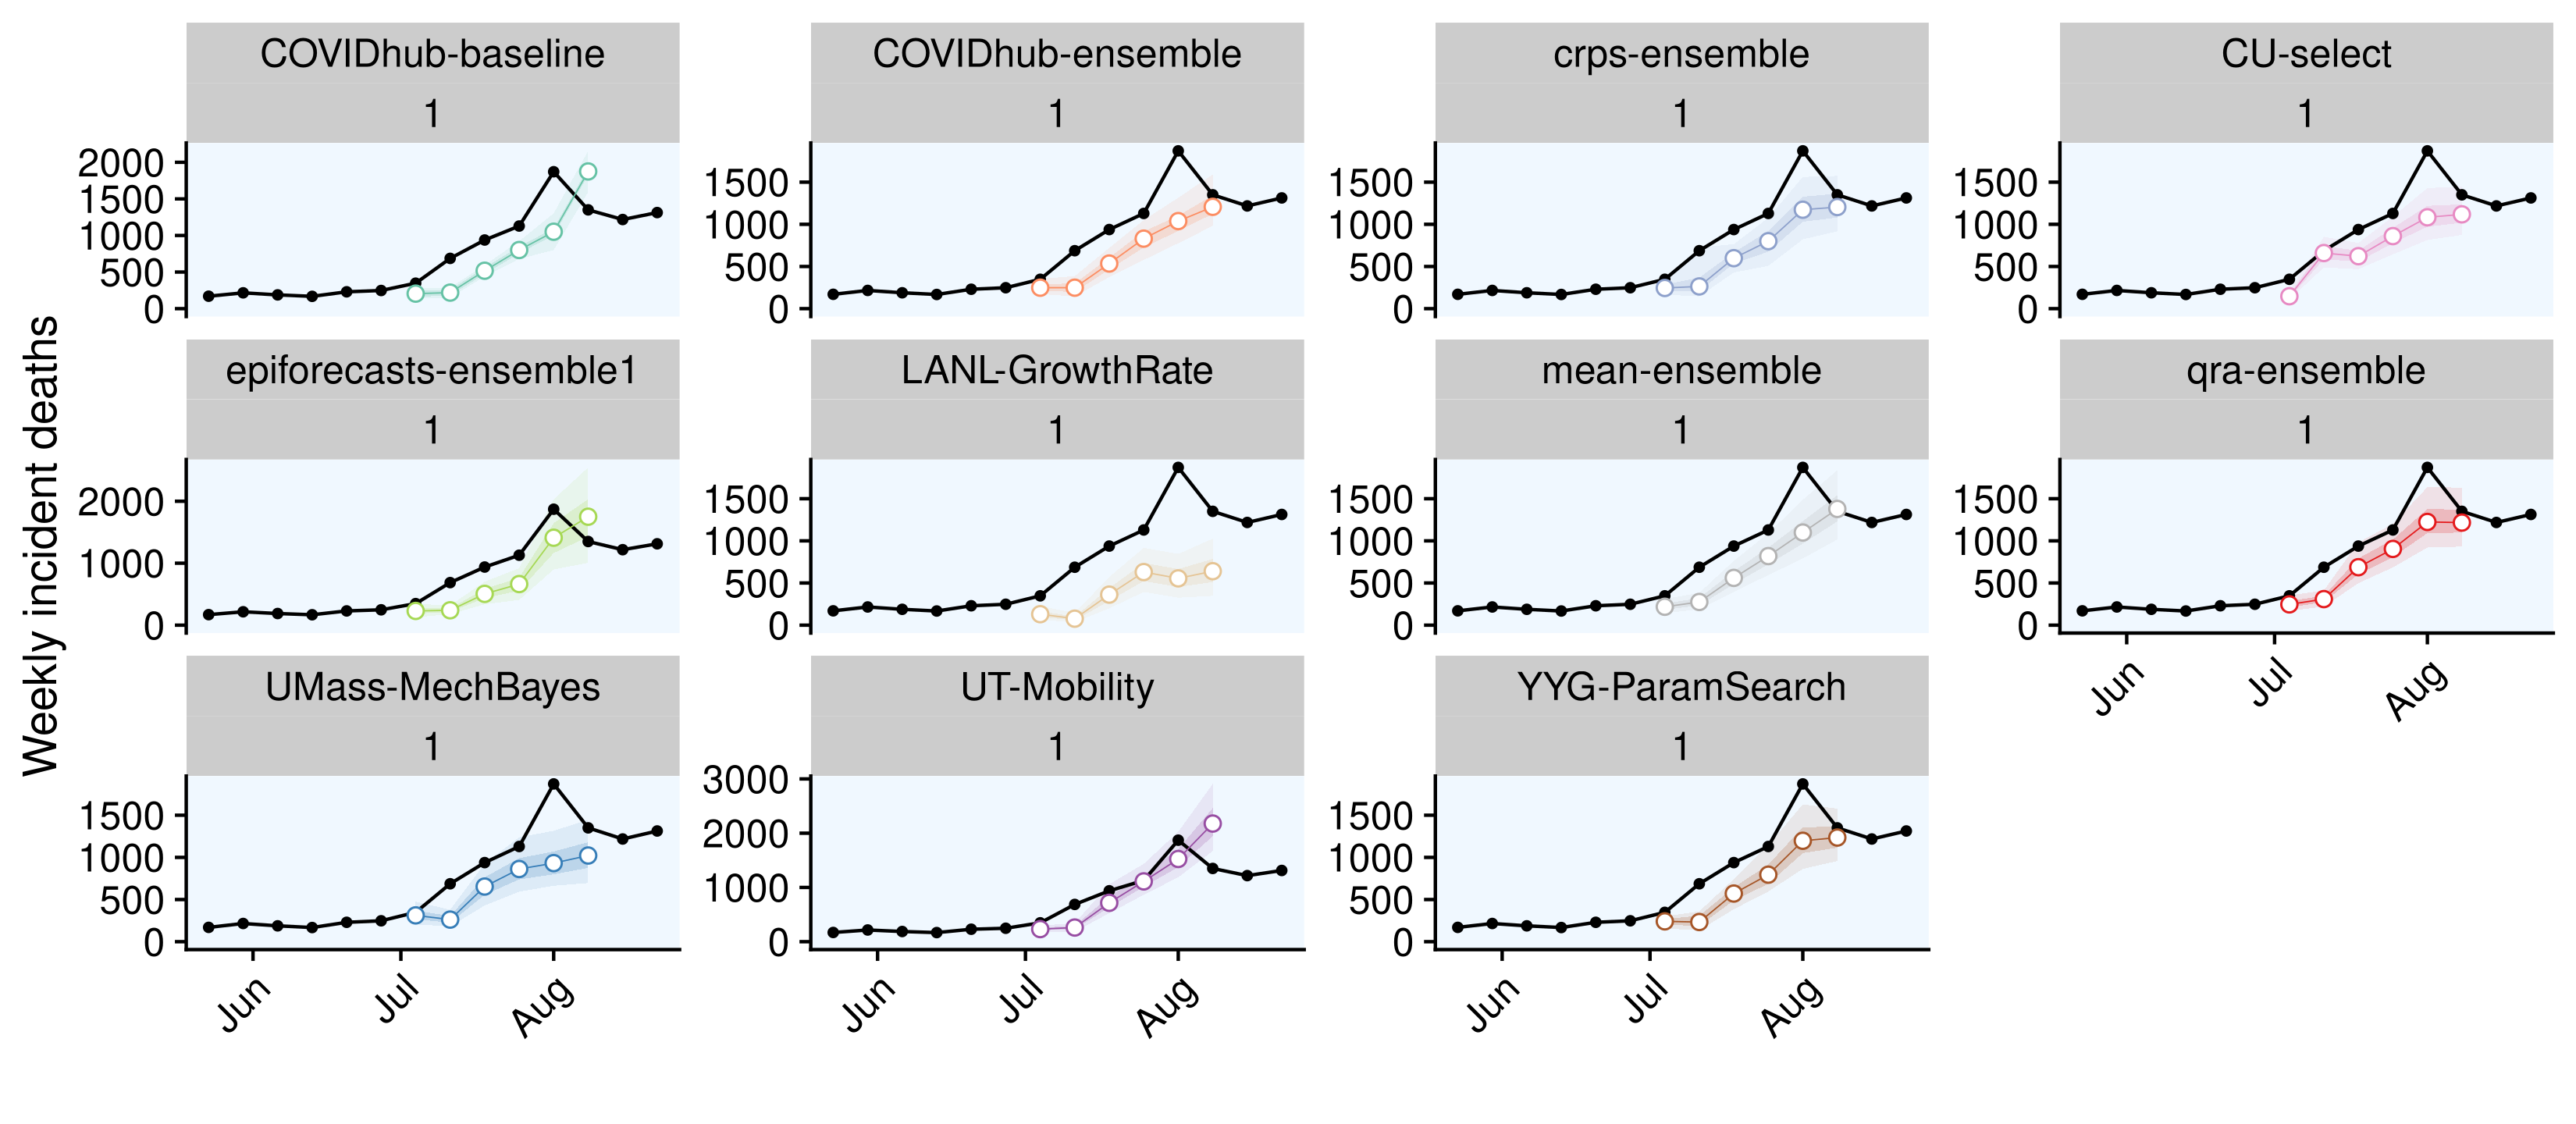
\includegraphics[width=1\linewidth]{../visualisation/chapter-5-results/scenario-baseline/Texas-one-week} \caption{One week ahead predictions and observed values in Texas}\label{fig:pred-texas}
\end{figure}

\hypertarget{pit-histograms}{%
\subsection{PIT histograms}\label{pit-histograms}}

In addition to looking at coverage plots, we can also approach calibration through PIT histograms. Figure \ref{all-pit-plots} shows the PIT histograms for all eleven models. We can immediately see that the Anderson-Darling test for uniformity is rejected for all models. While some models are indeed severely miscalibrated (as seen before in the coverage plots), we may probably also conclude that the Anderson-Darling test has limited value for most practical purposes of model comparison. PIT histograms are arguably somewhat hard to interpret for many readers. However, they provide a very good way to succinctly summarise different aspects of calibration and show again a lot of the things previously observed in other plots. We can for example see again the bias in the qra-ensemble and the YYG-ParamSearch model. Or we can recognise the hump shape corresponding to the positive coverage deviation of the crps-ensemble and the mean-ensemble (the predictions are wider than they actually need be). We will, however, not revisit all these aspects again, but instead turn to sharpness now.

\begin{figure}
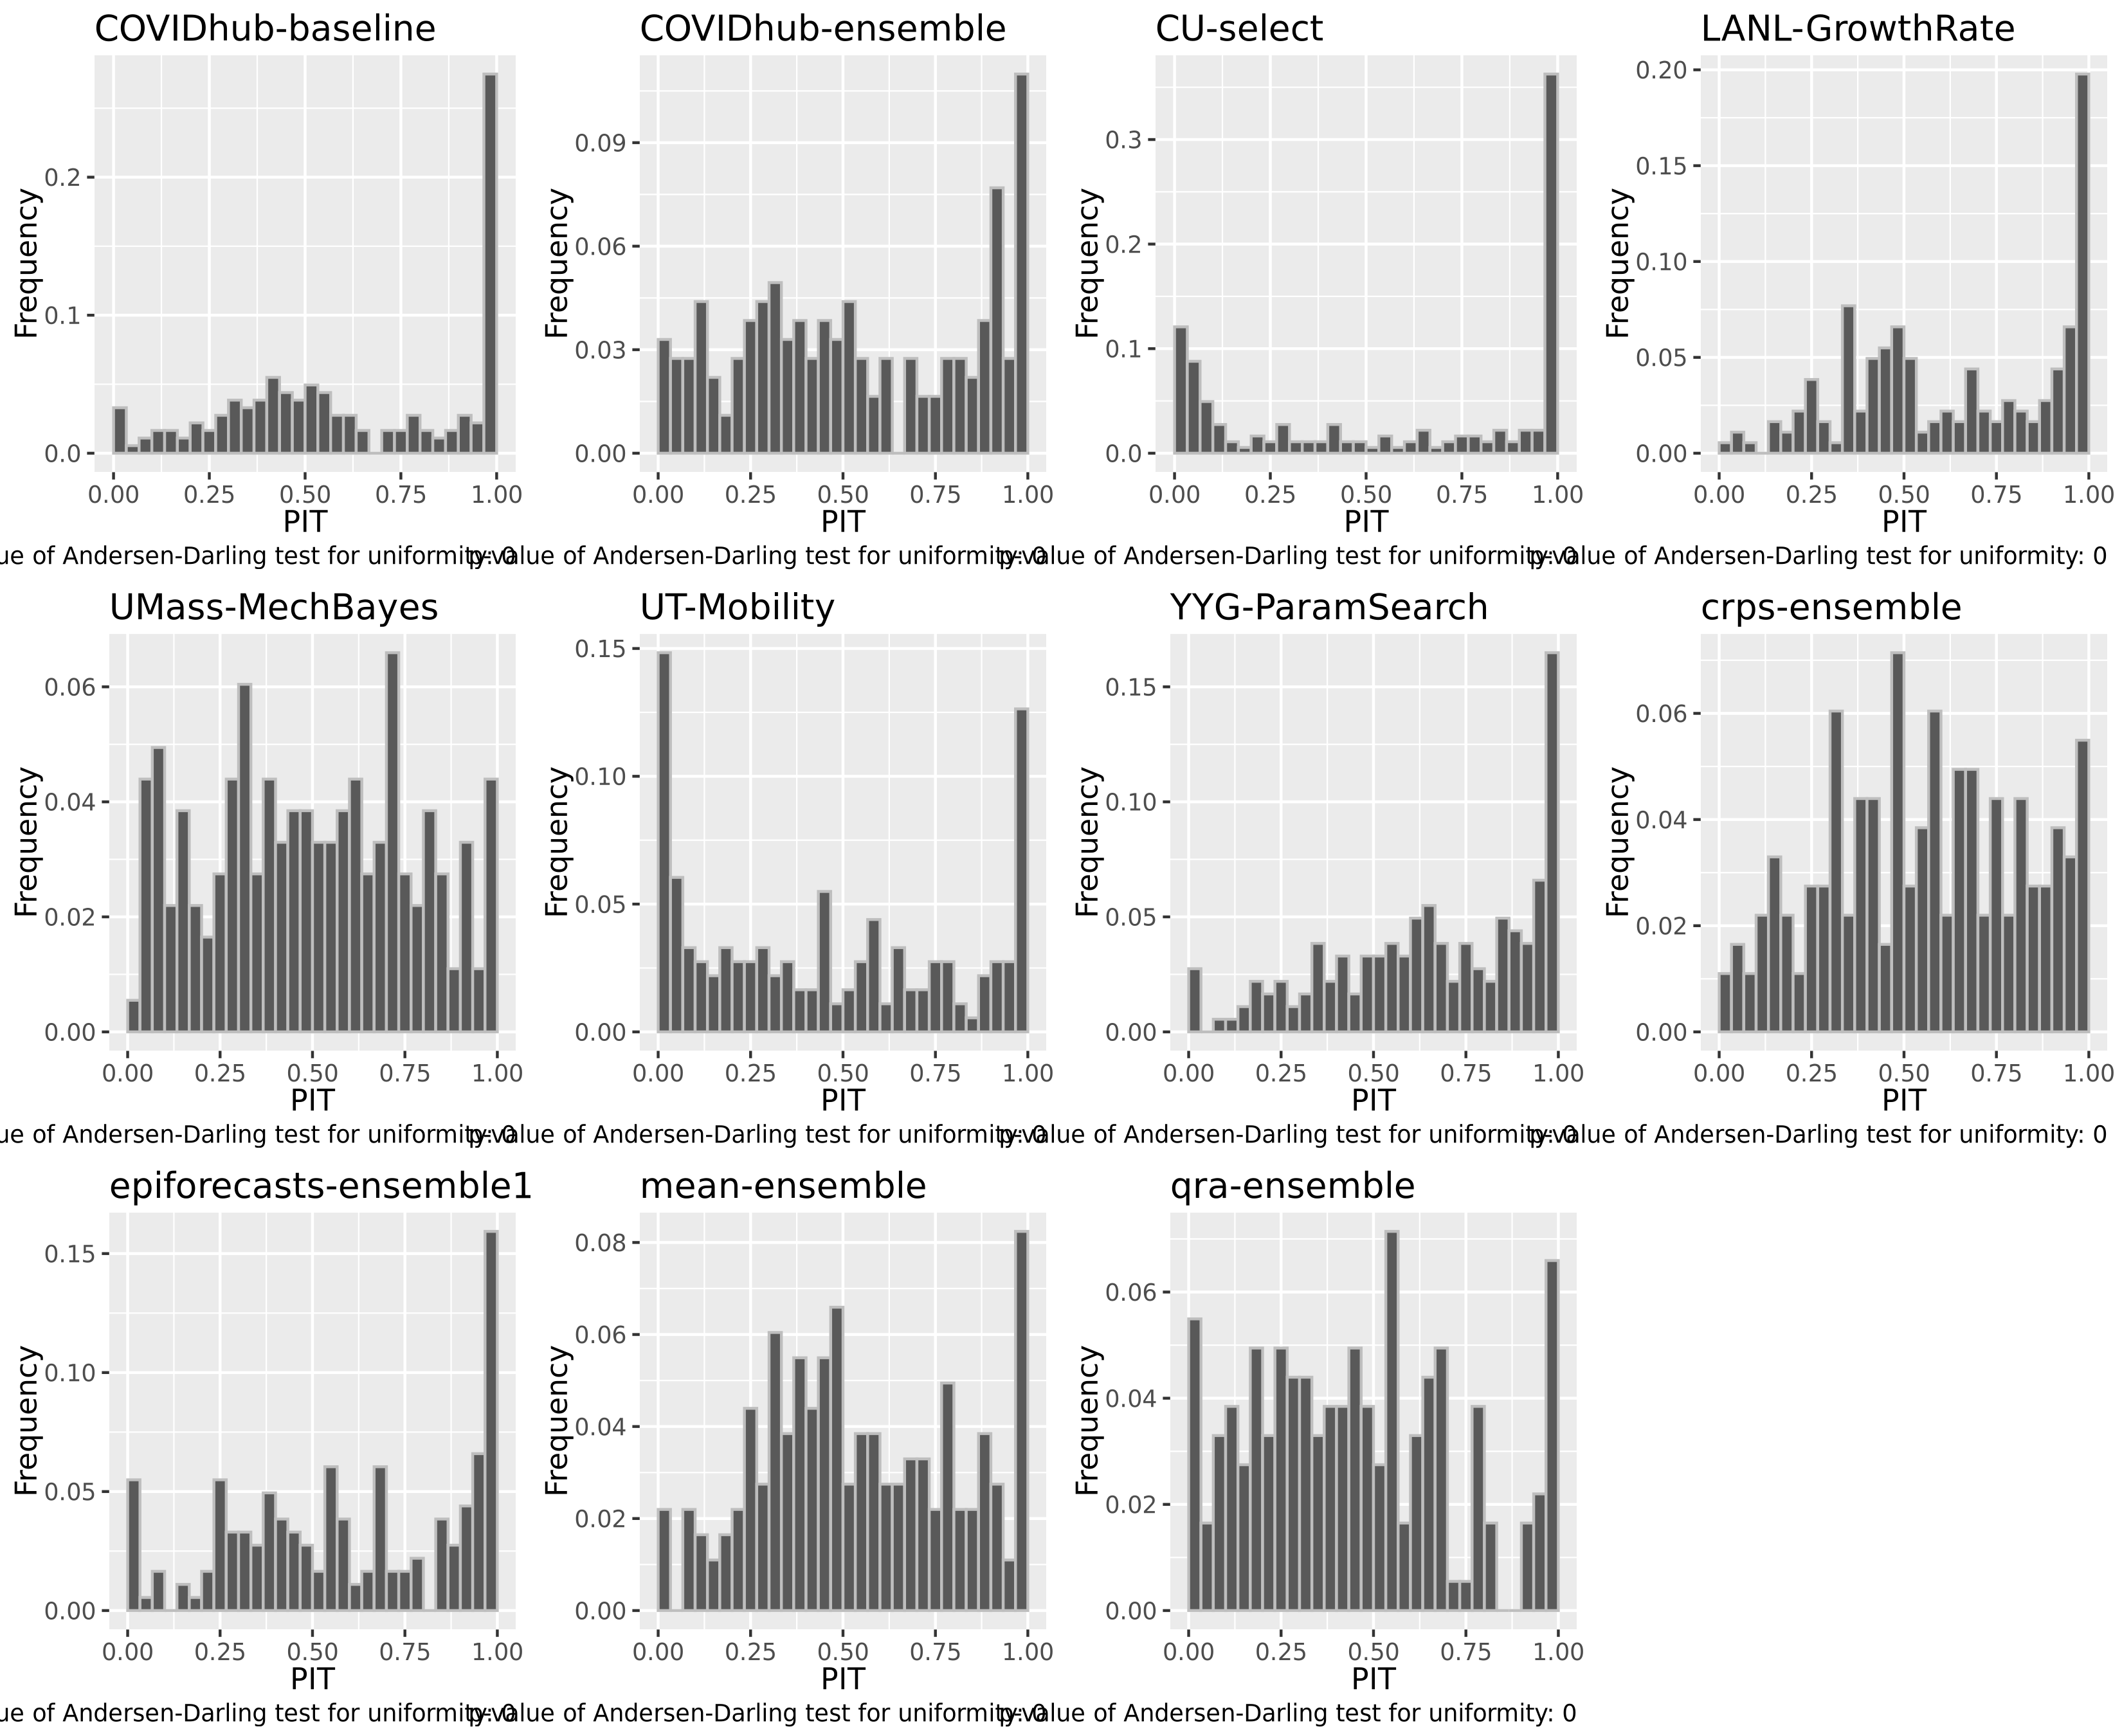
\includegraphics[width=1\linewidth]{../visualisation/chapter-5-results/all-pit-plots} \caption{PIT histograms for all models. Samples were obtained by first fitting a gamma distribution to the set of quantiles. Note that the PIT plots shown here don't have the same scale on the y-axis, which make them easier to read on their own, but a bit harder to compare. }\label{fig:all-pit-plots}
\end{figure}

\hypertarget{assessing-sharpness}{%
\section{Assessing sharpness}\label{assessing-sharpness}}

INTRODUCION TO SECTION

In order to understand the individual model better it is again most helpful to plot sharpness next to predictions. Figure \ref{fig:sharpness-crps-ensemble} does this for the crps-ensemble model for one-week-ahead predictions. Only one of the ensemble models is shown as all four make very similar forecasts. We can see that sharpness does not really follow a clearly identifiable pattern. It is much larger, of course, in locations like the US as a whole that have many more cases. But we cannot really see the ensemble model consistently adapting to past mistakes. Ideally, we would want a model to make wider predictions whenever predictions and observations do not match (for example, when the trend changes) and narrower ones when past predictions and observations have matched. Unfortunately, none of the original PLOT IN APPENDIX models really seems to exhibit that kind of behaviour and the ensemble is not able to mitigate this shortcoming. Instead we see rather random looking changes in sharpness (see e.g.~Arizona, US).

\begin{figure}
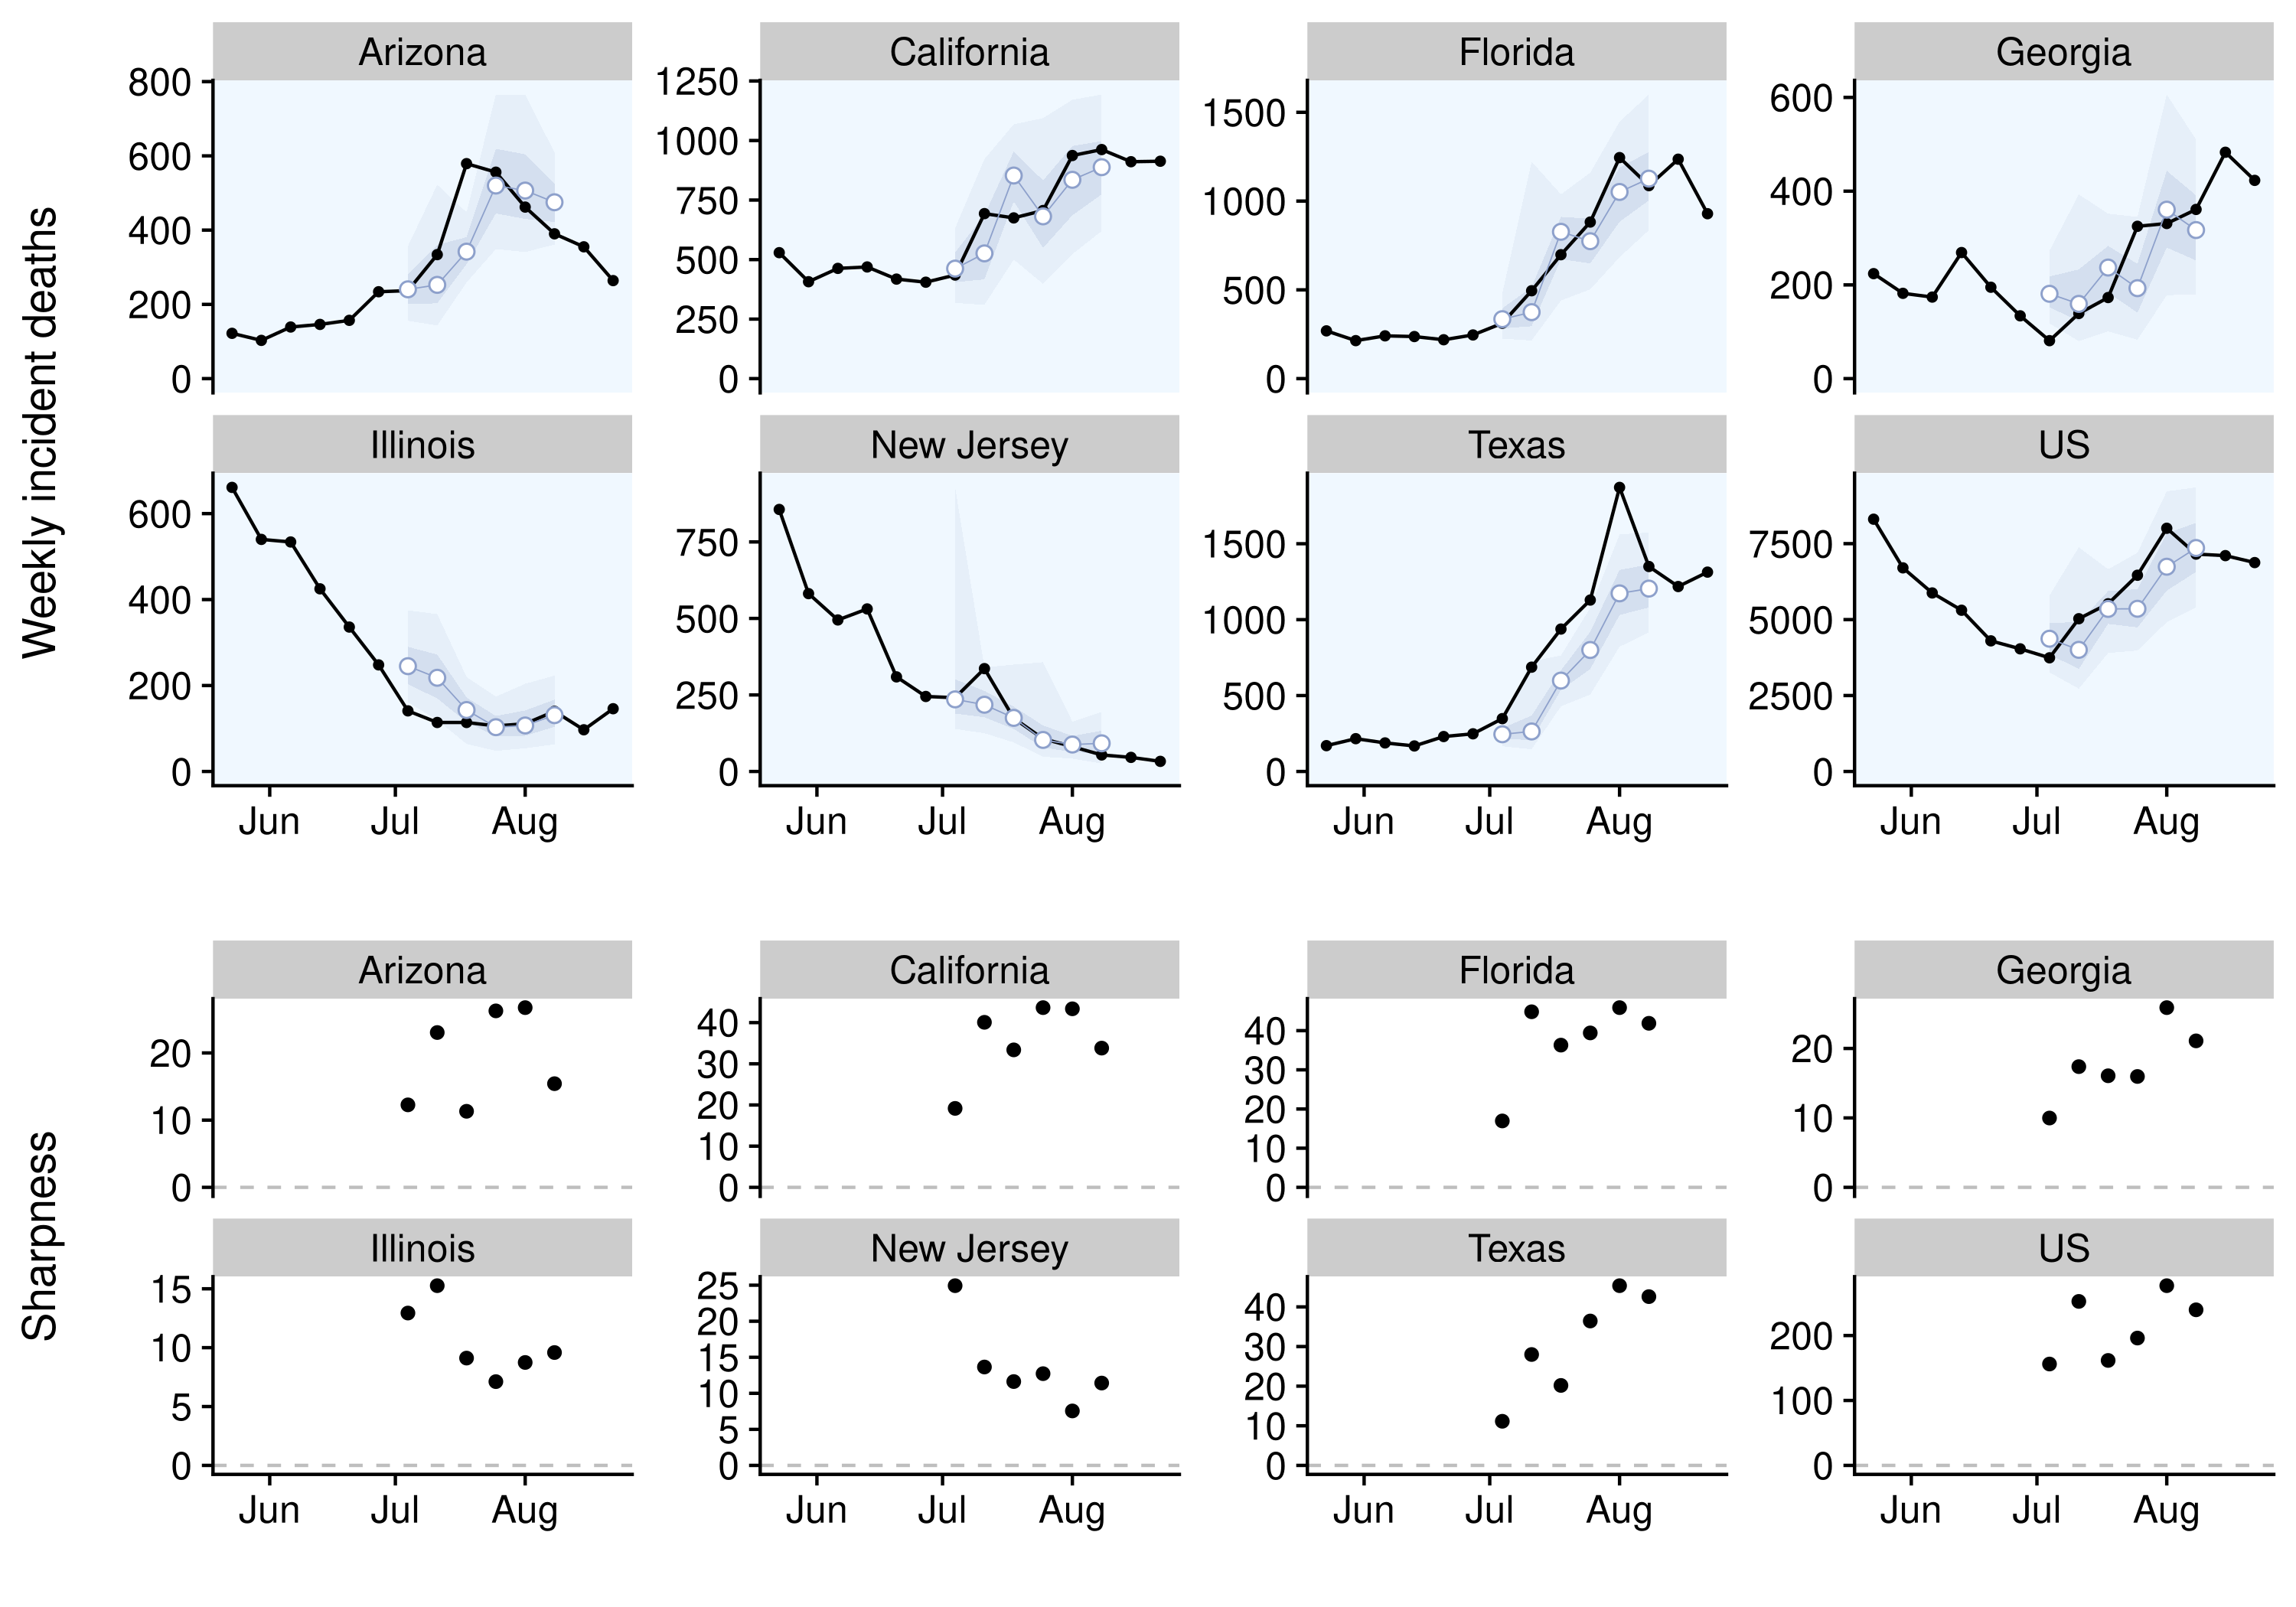
\includegraphics[width=1\linewidth]{../visualisation/chapter-5-results/scenario-baseline/sharpness-predictions-ensemble} \caption{Sharpness over different horizons. }\label{fig:sharpness-crps-ensemble}
\end{figure}

In order to get a better feeling for differences in model behaviour we can again try and compare sharpness in different subgroups. Figure \ref{fig:sharpness-horizons} shows sharpness over different horizons for all eleven models. This visualisation shows that prediction intervals tends to grow with increasing forecast horizons for almost all models. This provides a simple sanity check, as we should expect prediction intervals to grow with uncertainty. Only CU-select and LANL-GrowthRate fail this check as their median sharpness does not increase over all horizons. For the better performing models we mostly see a moderate increase with the only exception of UMass-MechBayes among the top performers. Comparing this with WIS over horizon (see Figure \ref{fig:heatmap-horizons}) we can conclude that this lack of sharpness for four-week-ahead forecasts is indeed accompanied by a worse weighted interval score. We can now also conclude that it is this lack of sharpness for four-week-ahead-predictions that cause UMass-MechBayes to rank among the bottom in terms of average sharpness (compare again Figure \ref{fig:coloured-summarised-scores}).

\begin{figure}
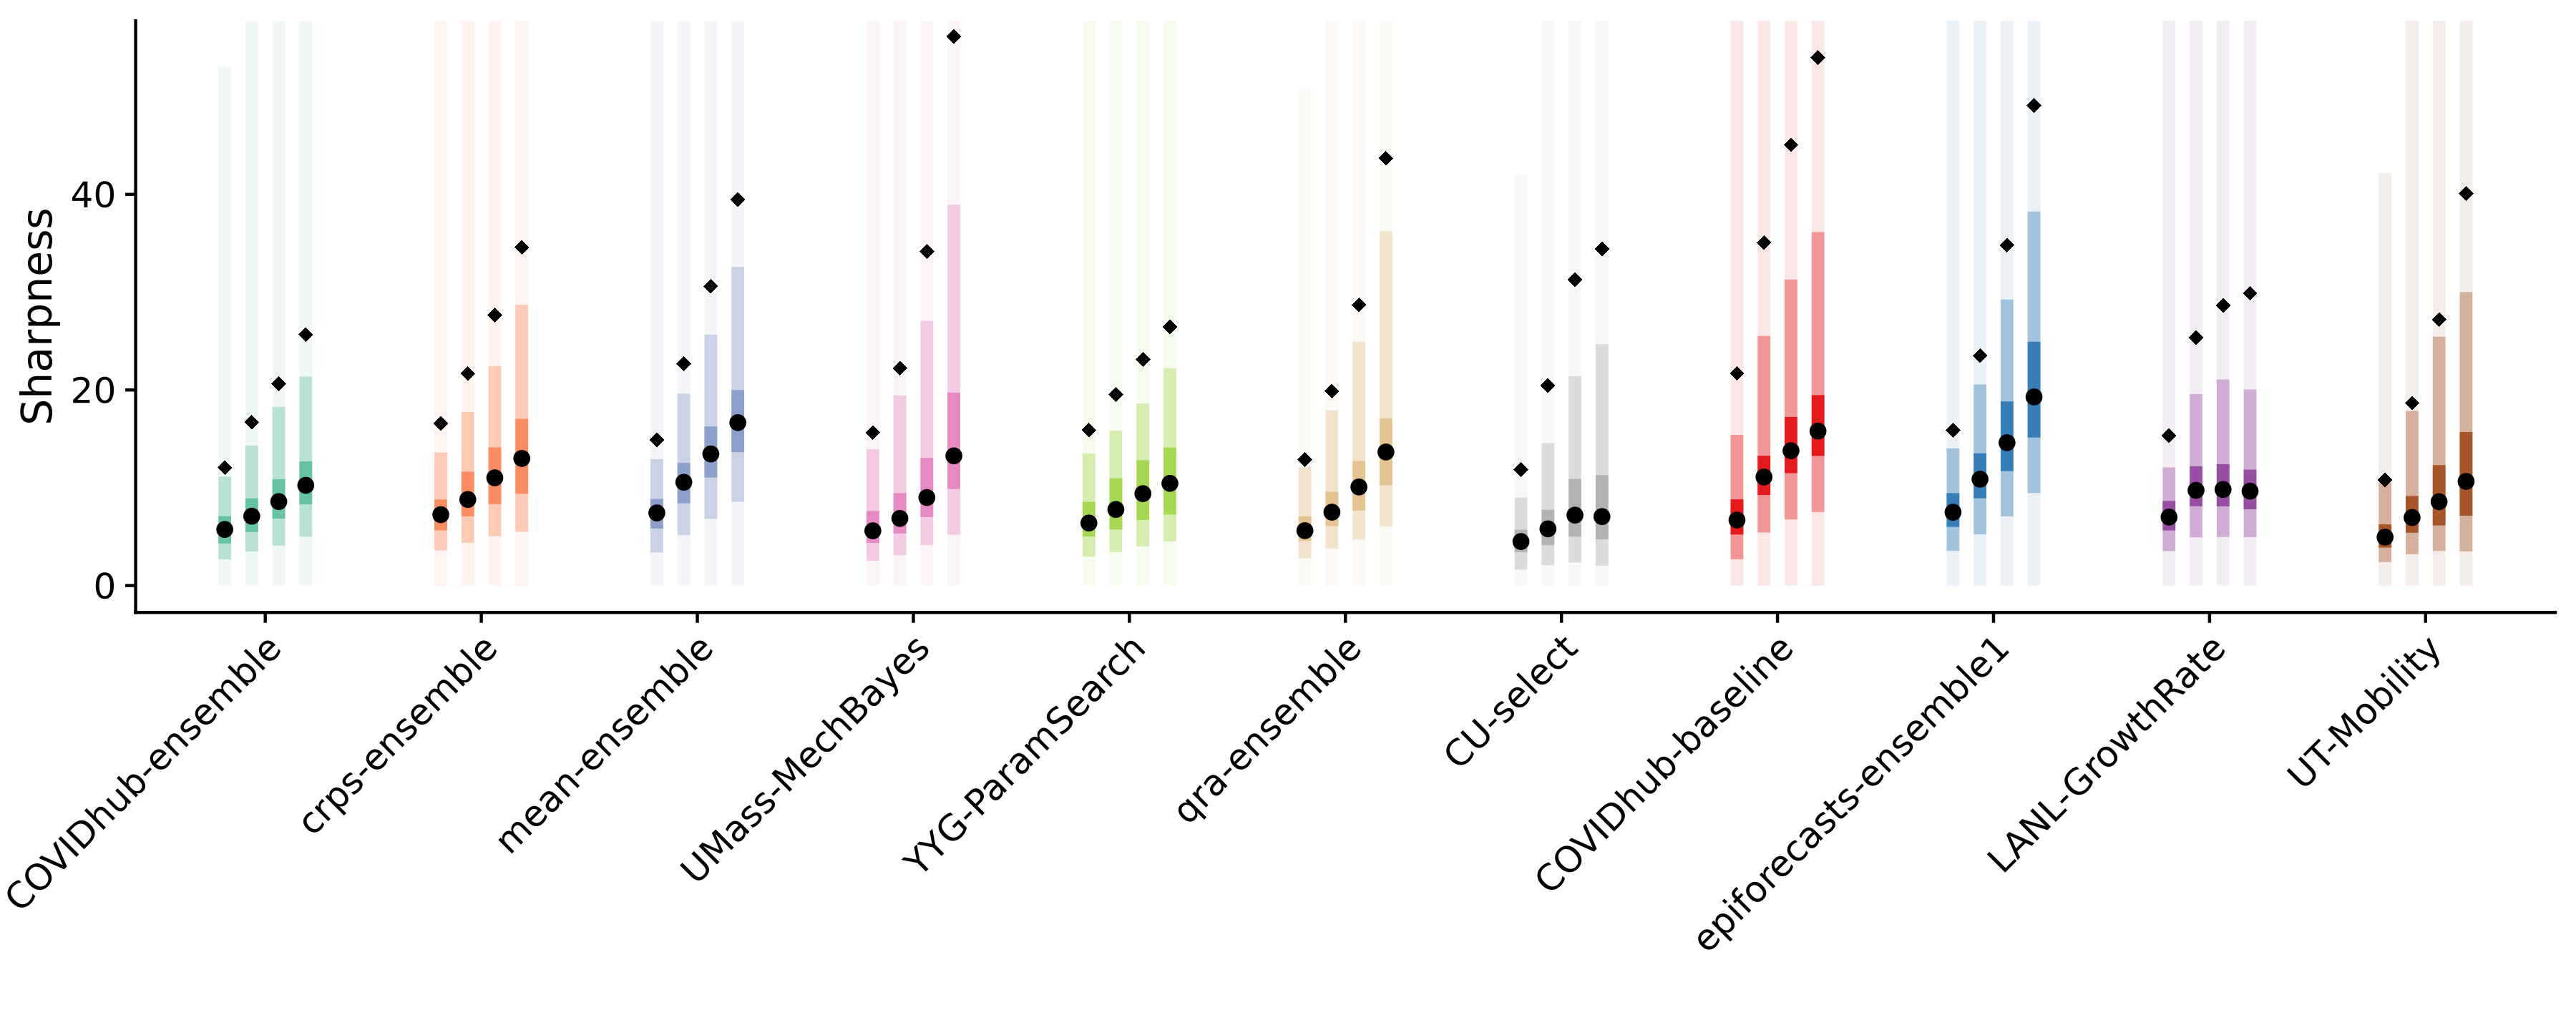
\includegraphics[width=1\linewidth]{../visualisation/chapter-5-results/sharpness-horizons} \caption{Sharpness over different horizons. }\label{fig:sharpness-horizons}
\end{figure}

Looking at sharpness separated by different interval ranges allows us again to discern the contributions to overall sharpness from individual prediction intervals. Figure \ref{fig:scores-ranges} the contributions from inner and outer prediction intervals for all eleven models. It generally seems that 50\% intervals tend to contribute most to sharpnes, while neither narrow intervals near the median nor the tails of the predictive distribution seem to make large contributions.

\begin{figure}
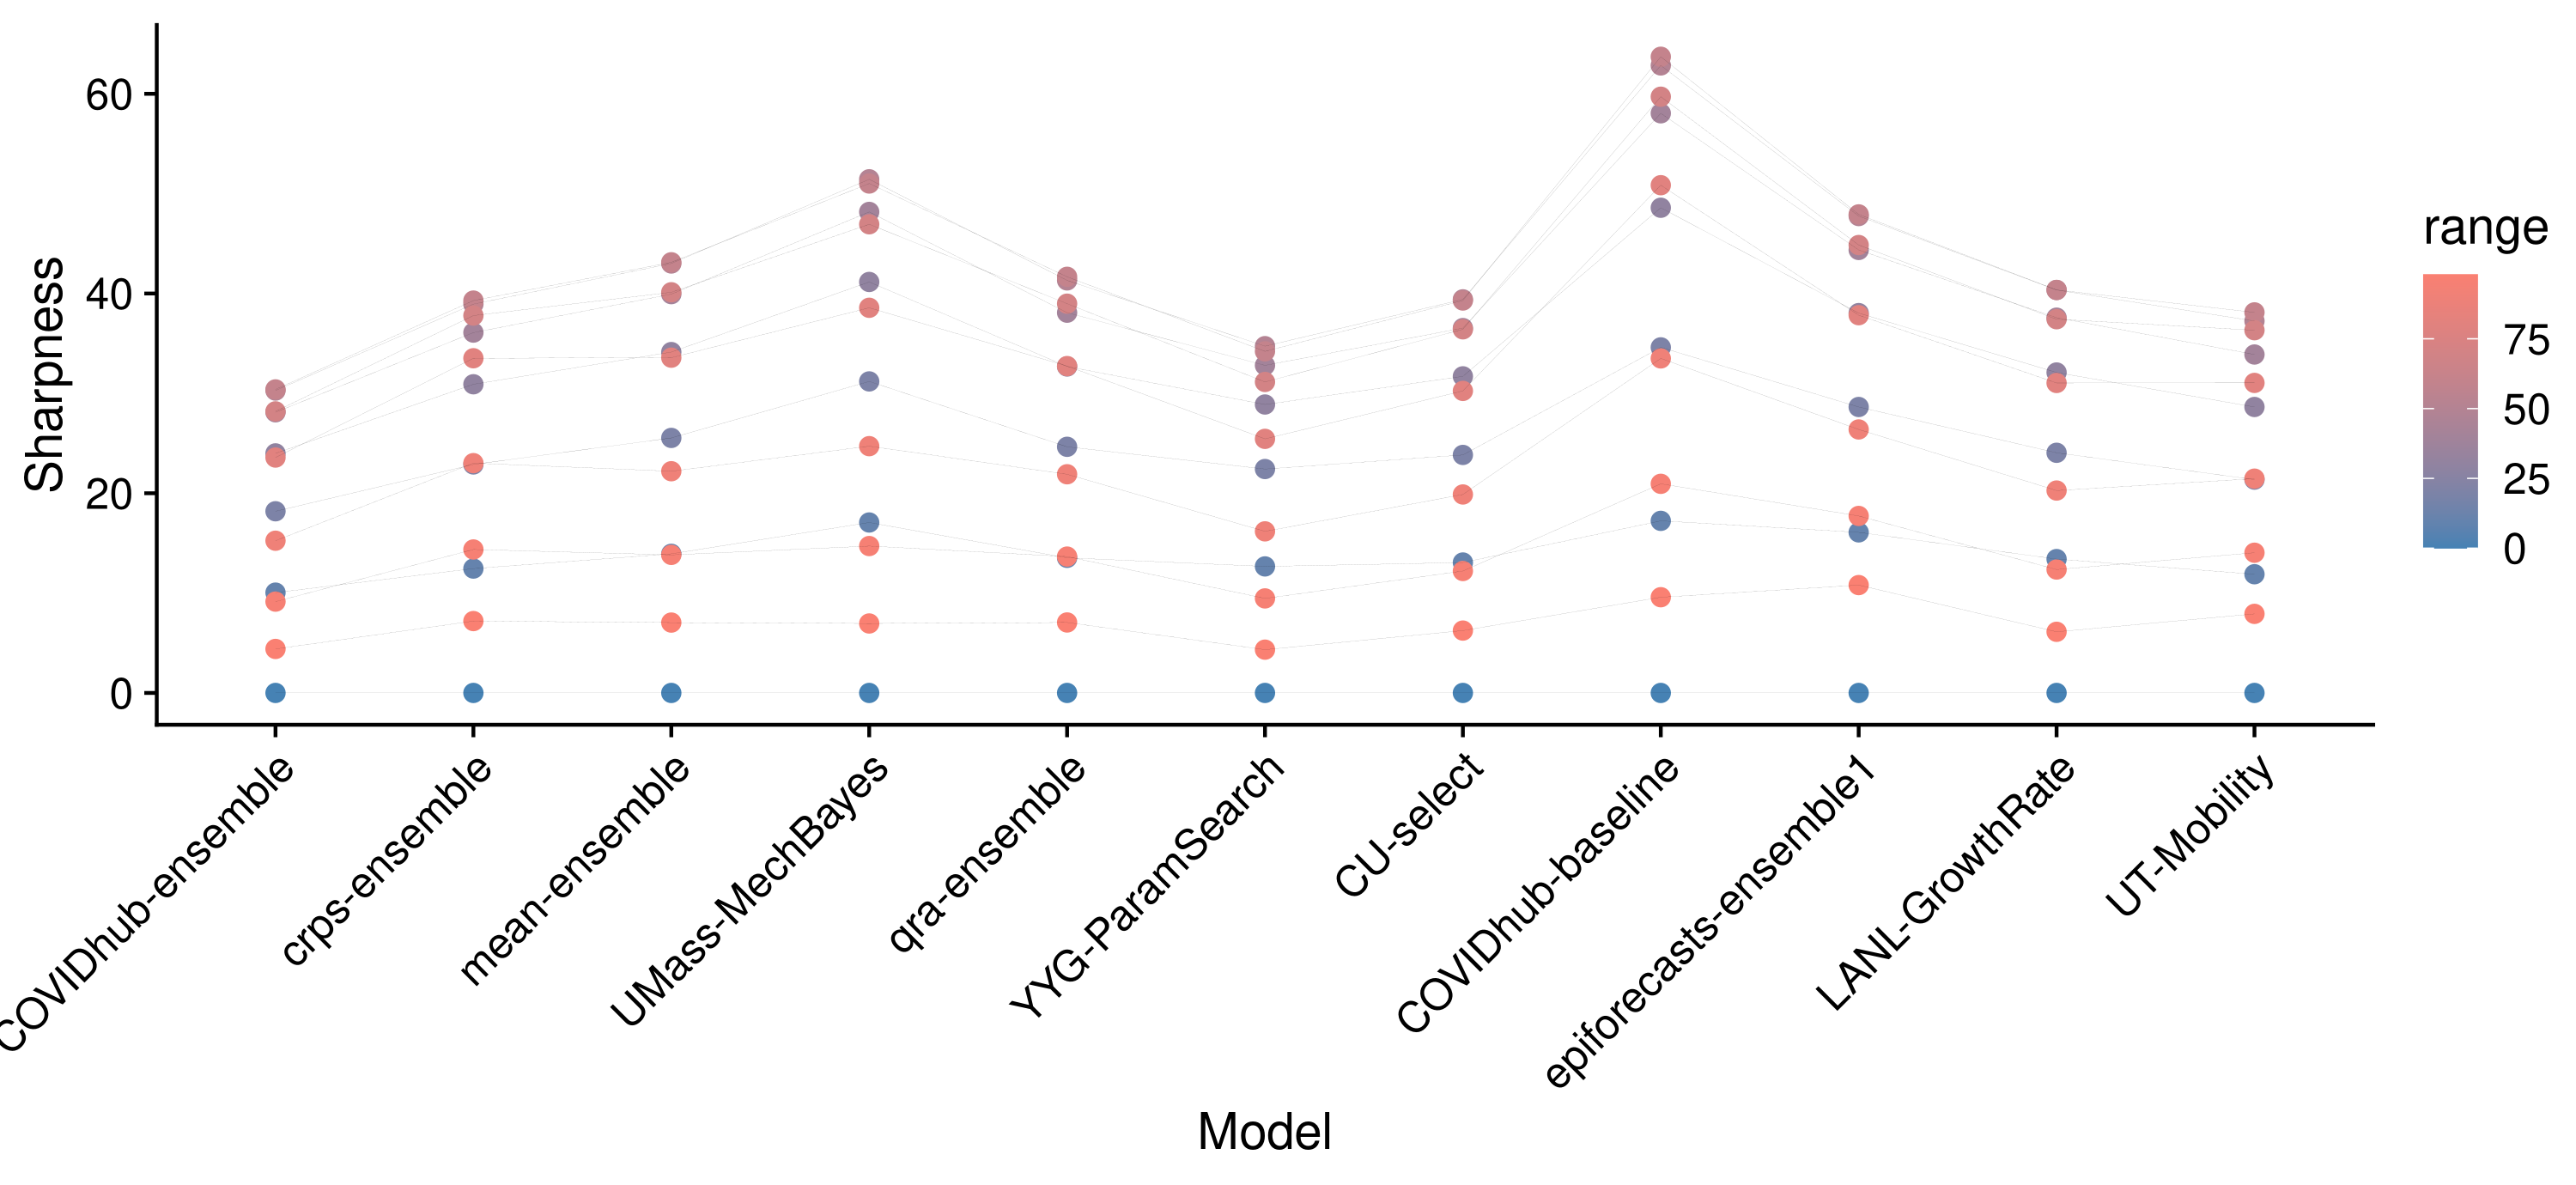
\includegraphics[width=1\linewidth]{../visualisation/chapter-5-results/sharpness-by-range} \caption{Sharpness across all states and forecast dates and horizons for different interval ranges}\label{fig:sharpness-ranges}
\end{figure}

Visualising sharpness for different states is again a way to see how different states vary in the sharpness they permit as well as how consistetnly models do in terms of sharpness. Figure \ref{fig:sharpness-ensemble} shows sharpness for every model and ensemble. We clearly see that average sharpness is largely dominated by sharpness in the US as a whole. We can also observe that some models (e.g.~COVIDhub-ensemble, YYG-ParamSearch, CU-select) consistently tend towards sharper forecasts, while other models vary a lot across regions.

\begin{figure}
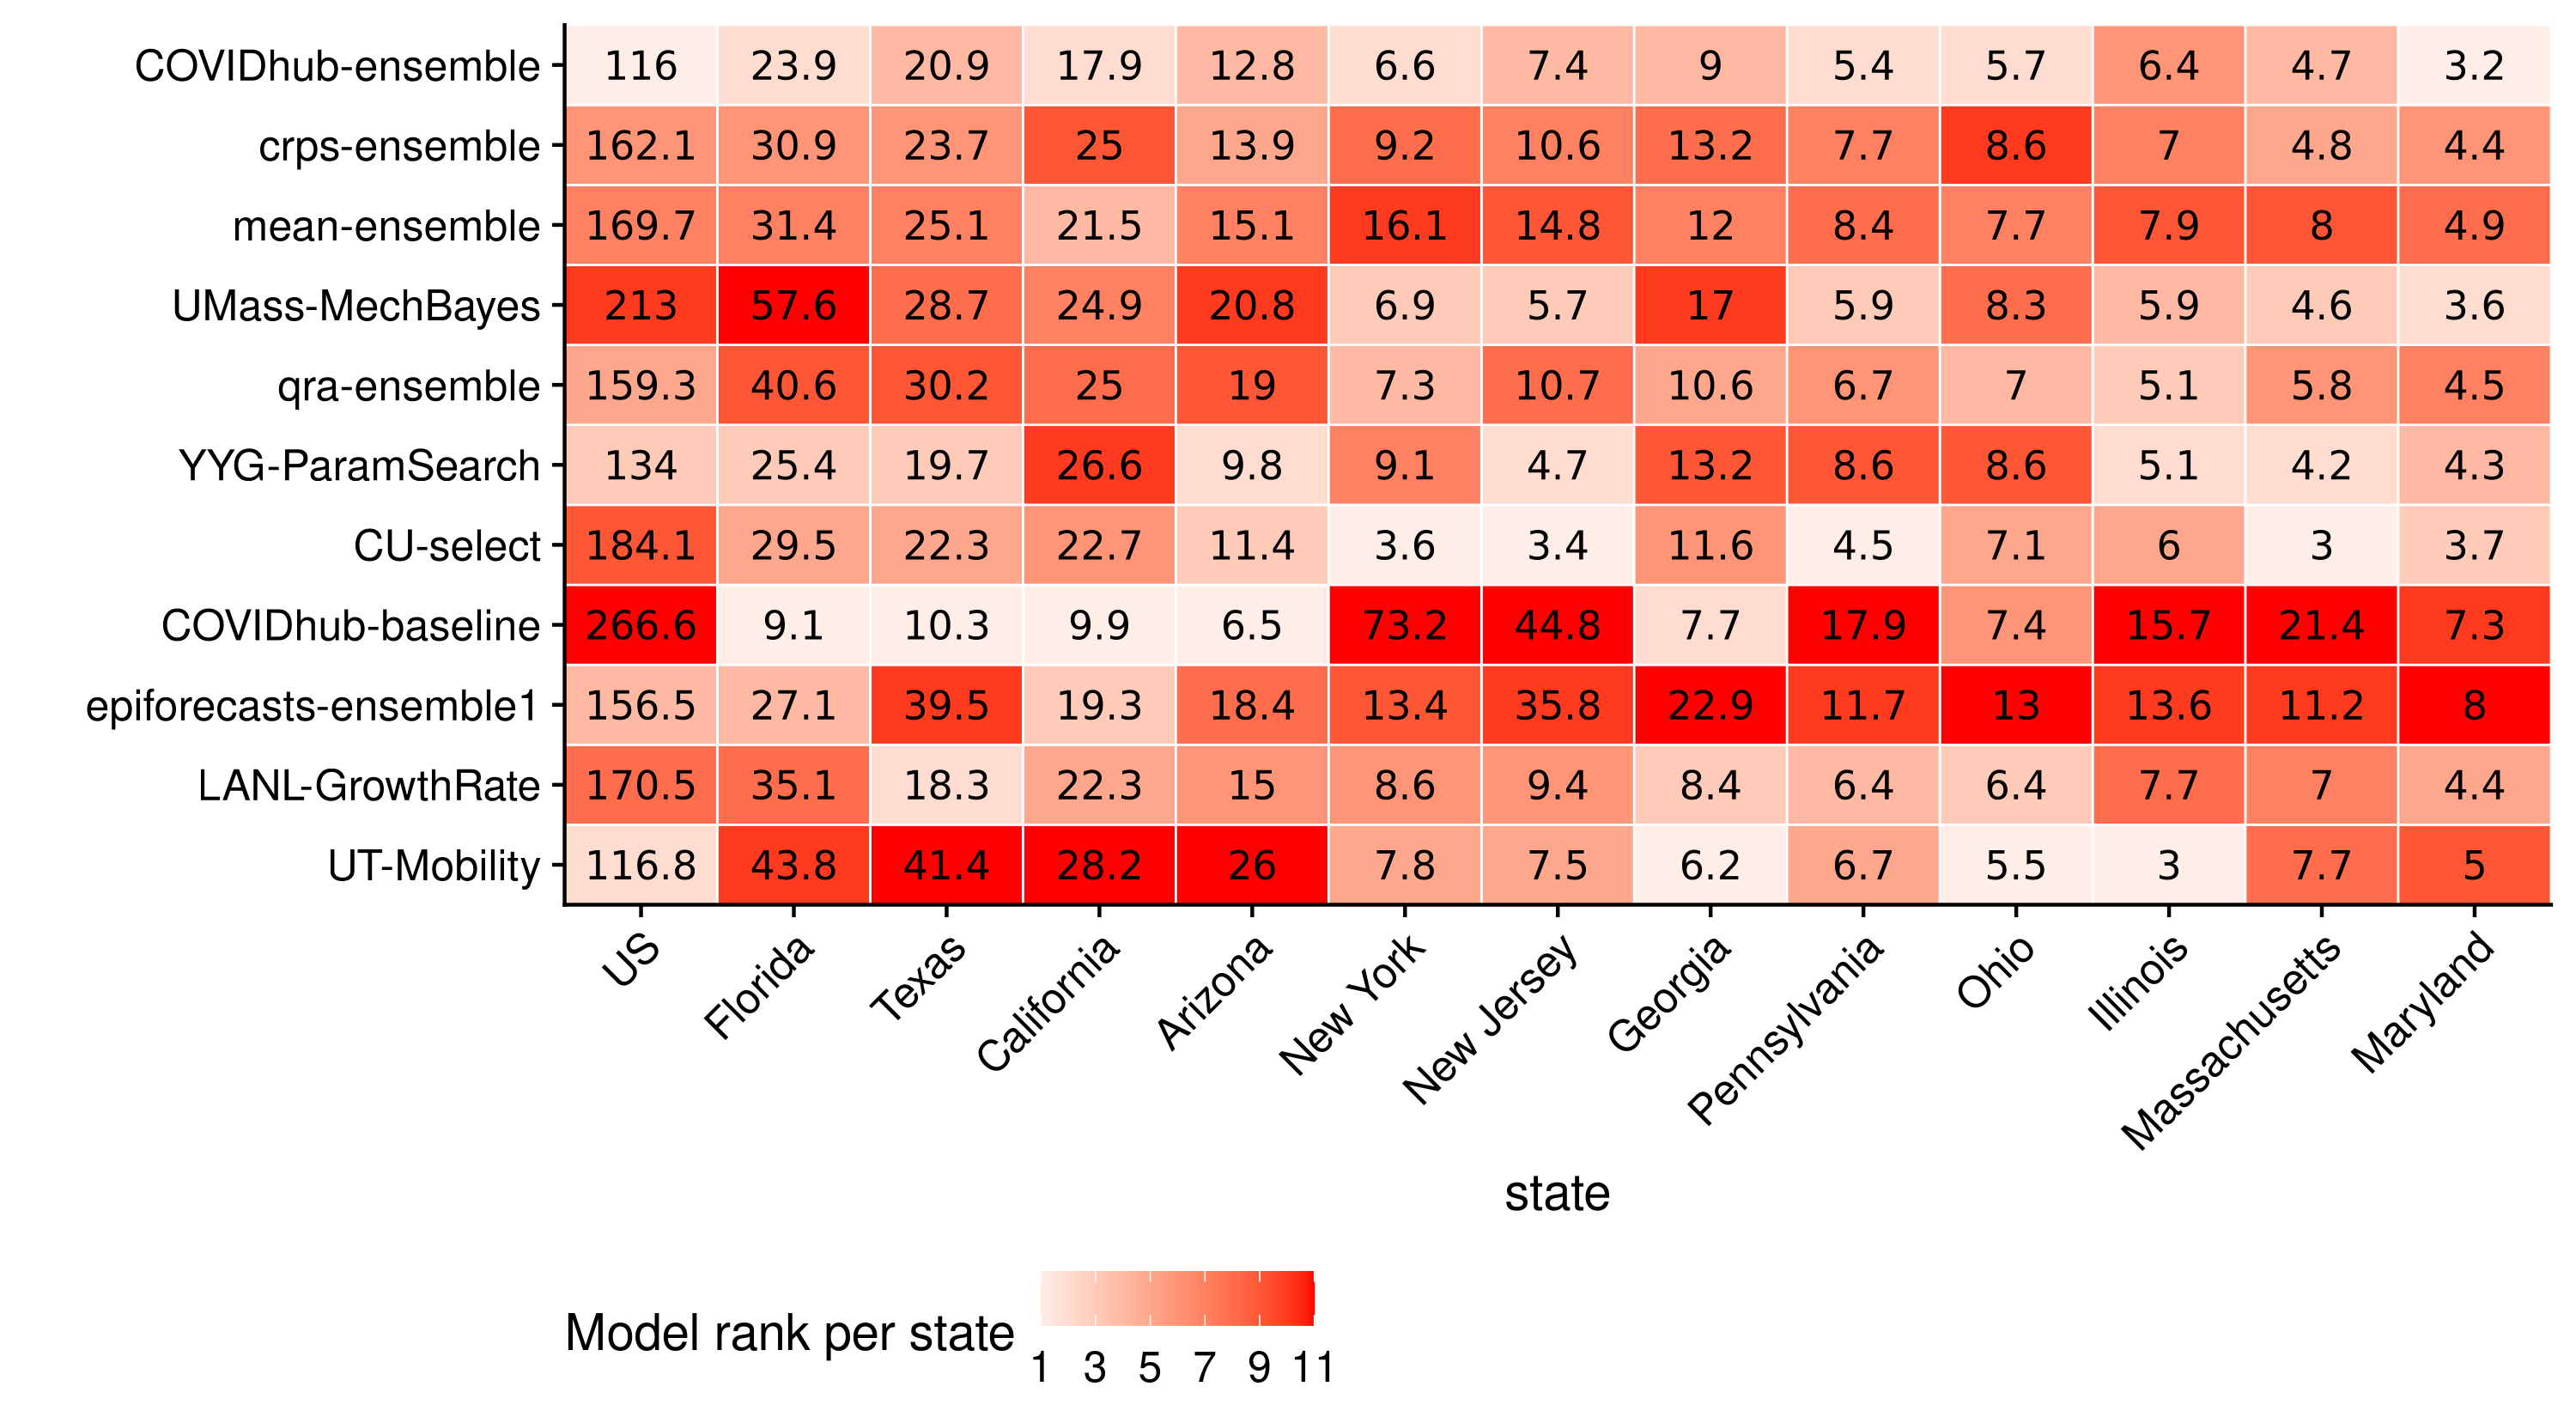
\includegraphics[width=1\linewidth]{../visualisation/chapter-5-results/scenario-baseline/heatmap-model-sharpness} \caption{Sharpness of the ensemble models in different states. The shading indicates how much higher a certain sharpness value is compared to the minimum value achieved in that state.}\label{fig:sharpness-ensemble}
\end{figure}

SECTION SUMMARY?

\hypertarget{model-evaluation-in-a-regression-framework}{%
\section{Model evaluation in a regression framework}\label{model-evaluation-in-a-regression-framework}}

To complement the analysis presented above we can look at evaluation in a regression. This is a natural next steps towards model selection that in principle allows us to make a better founded decision for or against a specific model to choose for future predictions. It is also very helpful for the case in which we do not have a complete set of predictions. If a certain research group for example misses a submission or does not submit forecasts in all states, then we can better mitigate this in a regression framework than by merely averaging over all available data.

To that end we employ a mixed-effects model with fixed effects for models and horizons and random effects for states and forecast dates. The model formula looks as shown below. Interval scores are again log transformed to mitigate issues with the heavy tails of the original distribution. As a baseline we take the COVIDhub-ensemble model (the top performer). This helps us to discern whether models at the top can actually be distinguished and show significant performance differences.

\begin{Shaded}
\begin{Highlighting}[]
\NormalTok{fit \textless{}{-}}\StringTok{ }\NormalTok{lme4}\OperatorTok{::}\KeywordTok{lmer}\NormalTok{(log\_scores }\OperatorTok{\textasciitilde{}}\StringTok{ }\NormalTok{model }\OperatorTok{+}\StringTok{ }\NormalTok{horizon }\OperatorTok{+}\StringTok{ }\NormalTok{(}\DecValTok{1}\OperatorTok{|}\NormalTok{state) }\OperatorTok{+}\StringTok{ }\NormalTok{(}\DecValTok{1}\OperatorTok{|}\NormalTok{forecast\_date),}
                  \DataTypeTok{data =}\NormalTok{ unsummarised\_scores)}
\end{Highlighting}
\end{Shaded}

Table \ref{tab:random-effects-model} shows the results from that regression. We can see that the regression confirms general tendencies observed before. The horizon, for example, has a highly significant positive effect on the weighted interval score. The overall ranking of model effects corresponds to the model ranking by log interval score presented in \ref{fig:coloured-summarised-scores}. This regression can of course be adapted. One possibility is to model an interaction between model and horizon to control for the fact that some models cope better or worse with increasing uncertainty. It also seems sensible to model horizon as a factor instead of a metric variable. If we were especially interested in performance over say a four-week-ahead horizon, we could then estimate a separate effect for every model at horizon four by looking at the combination of the model effect and the interaction. The regression outcome suggests a clear split between two groups of models in terms of perfomance. Models in the top group are roughly comparable, except for the mean ensemble (and maybe the qra-ensemble) which fare a bit worse. Note again that the regression was performed on log scores which changes the order with respect to untransformed scores. The mean-ensemble, for example looks worse according to log scores than it would otherwise have. This suggests that mean-ensemble avoids outliers, but does a bit worse on a typical forecast.

\begin{table}

\caption{\label{tab:random-effects-model}Mixed model regression of the log weighted interval score on model, horizon (both fixed), state, and forecast date (both random)}
\centering
\resizebox{\linewidth}{!}{
\begin{tabular}[t]{lrrrrr}
\toprule
  & Estimate & Std. Error & df & t value & Pr(>|t|)\\
\midrule
(Intercept) & 3.1751929 & 0.3315952 & 12.8892 & 9.5755102 & 0.0000003\\
modelcrps-ensemble & 0.0791488 & 0.0590696 & 3259.8901 & 1.3399250 & 0.1803631\\
modelmean-ensemble & 0.1787953 & 0.0590696 & 3259.8901 & 3.0268573 & 0.0024904\\
modelUMass-MechBayes & 0.0645586 & 0.0590696 & 3259.8901 & 1.0929249 & 0.2745075\\
modelqra-ensemble & 0.1096244 & 0.0590696 & 3259.8901 & 1.8558514 & 0.0635649\\
\addlinespace
modelYYG-ParamSearch & 0.0563939 & 0.0590696 & 3259.8901 & 0.9547021 & 0.3397992\\
modelCU-select & 0.5842311 & 0.0590696 & 3259.8901 & 9.8905536 & 0.0000000\\
modelCOVIDhub-baseline & 0.7578785 & 0.0590696 & 3259.8901 & 12.8302623 & 0.0000000\\
modelepiforecasts-ensemble1 & 0.5177092 & 0.0590696 & 3259.8901 & 8.7643931 & 0.0000000\\
modelLANL-GrowthRate & 0.4618302 & 0.0590696 & 3259.8901 & 7.8184070 & 0.0000000\\
\addlinespace
modelUT-Mobility & 0.5969057 & 0.0590696 & 3259.8901 & 10.1051247 & 0.0000000\\
horizon & 0.2421870 & 0.0116076 & 3262.1356 & 20.8645833 & 0.0000000\\
\bottomrule
\end{tabular}}
\end{table}

While the strength of this regression framework is its ability to aid with model selection, we can also use it to learn more about the effects of different locations and forecast dates. Figure \ref{fig:random-effects} shows the estimated random effects from all different locations and forecast dates. We can see that location effects are much larger than forecast date effects.

\begin{figure}
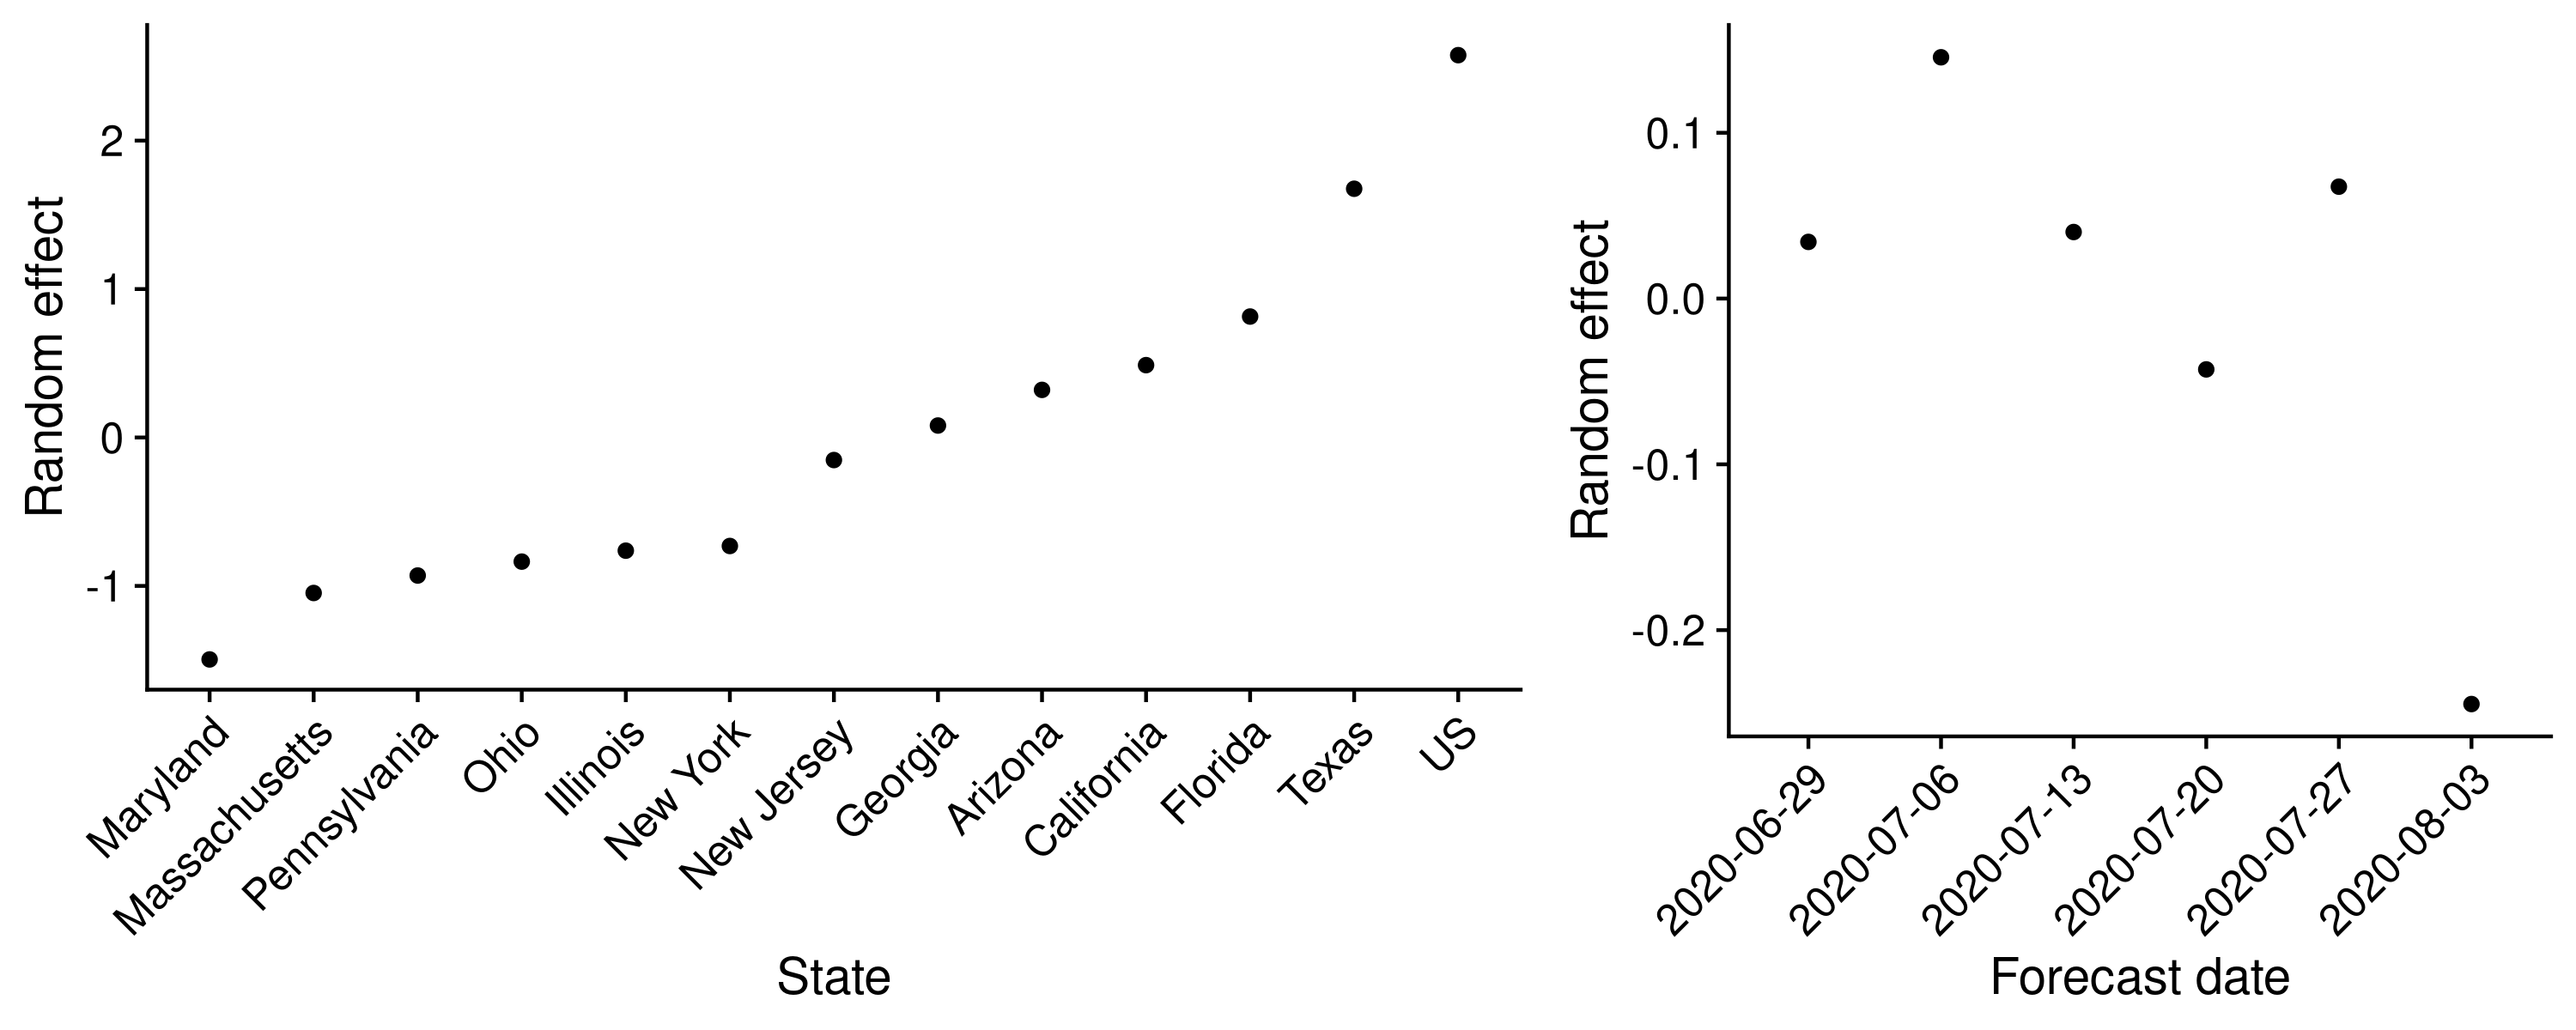
\includegraphics[width=1\linewidth]{../visualisation/chapter-5-results/random-effects} \caption{Random effects of the different locations (left) and forecast dates (right}\label{fig:random-effects}
\end{figure}

SECTION SUMMARY / TRANSITION

\hypertarget{assessing-ensemble-performance}{%
\section{Assessing ensemble performance}\label{assessing-ensemble-performance}}

The following section will explore some aspects concerning the ensemble models in a bit more detail. These paragraphs will focus on the qra and the crps ensemble, as these are the ones of greatest interest. The first part will examine how ensemble member weights evolve over time for the two model aggregation approaches. The second part will then look at different variants of the qra and crps ensemble that alter the number of past observations to take into account or the horizon to optimise for. A regression framework will be used again to determine differences between the different ensemble variants. The COVIDhub-ensemble will here serve as a benchmark against which to compare the other ensembles.

The mean-ensemble will not be discussed in more depth as it is not very interesting in terms of further investigation. Since its member models are all already included in the COVIDhub-ensemble model, performance differences between the mean-ensemble and the COVIDhub-ensemble can be fully attributed to the subselection of models from the Forecast Hub for this thesis.

\hypertarget{model-weights-over-time}{%
\subsection{Model weights over time}\label{model-weights-over-time}}

Looking at the how ensemble weights evolve over time can give us insights about how the ensembles work. Figure \ref{fig:weights-time} visualises this evolution. We can see that both model aggregation approaches seem to

\begin{figure}
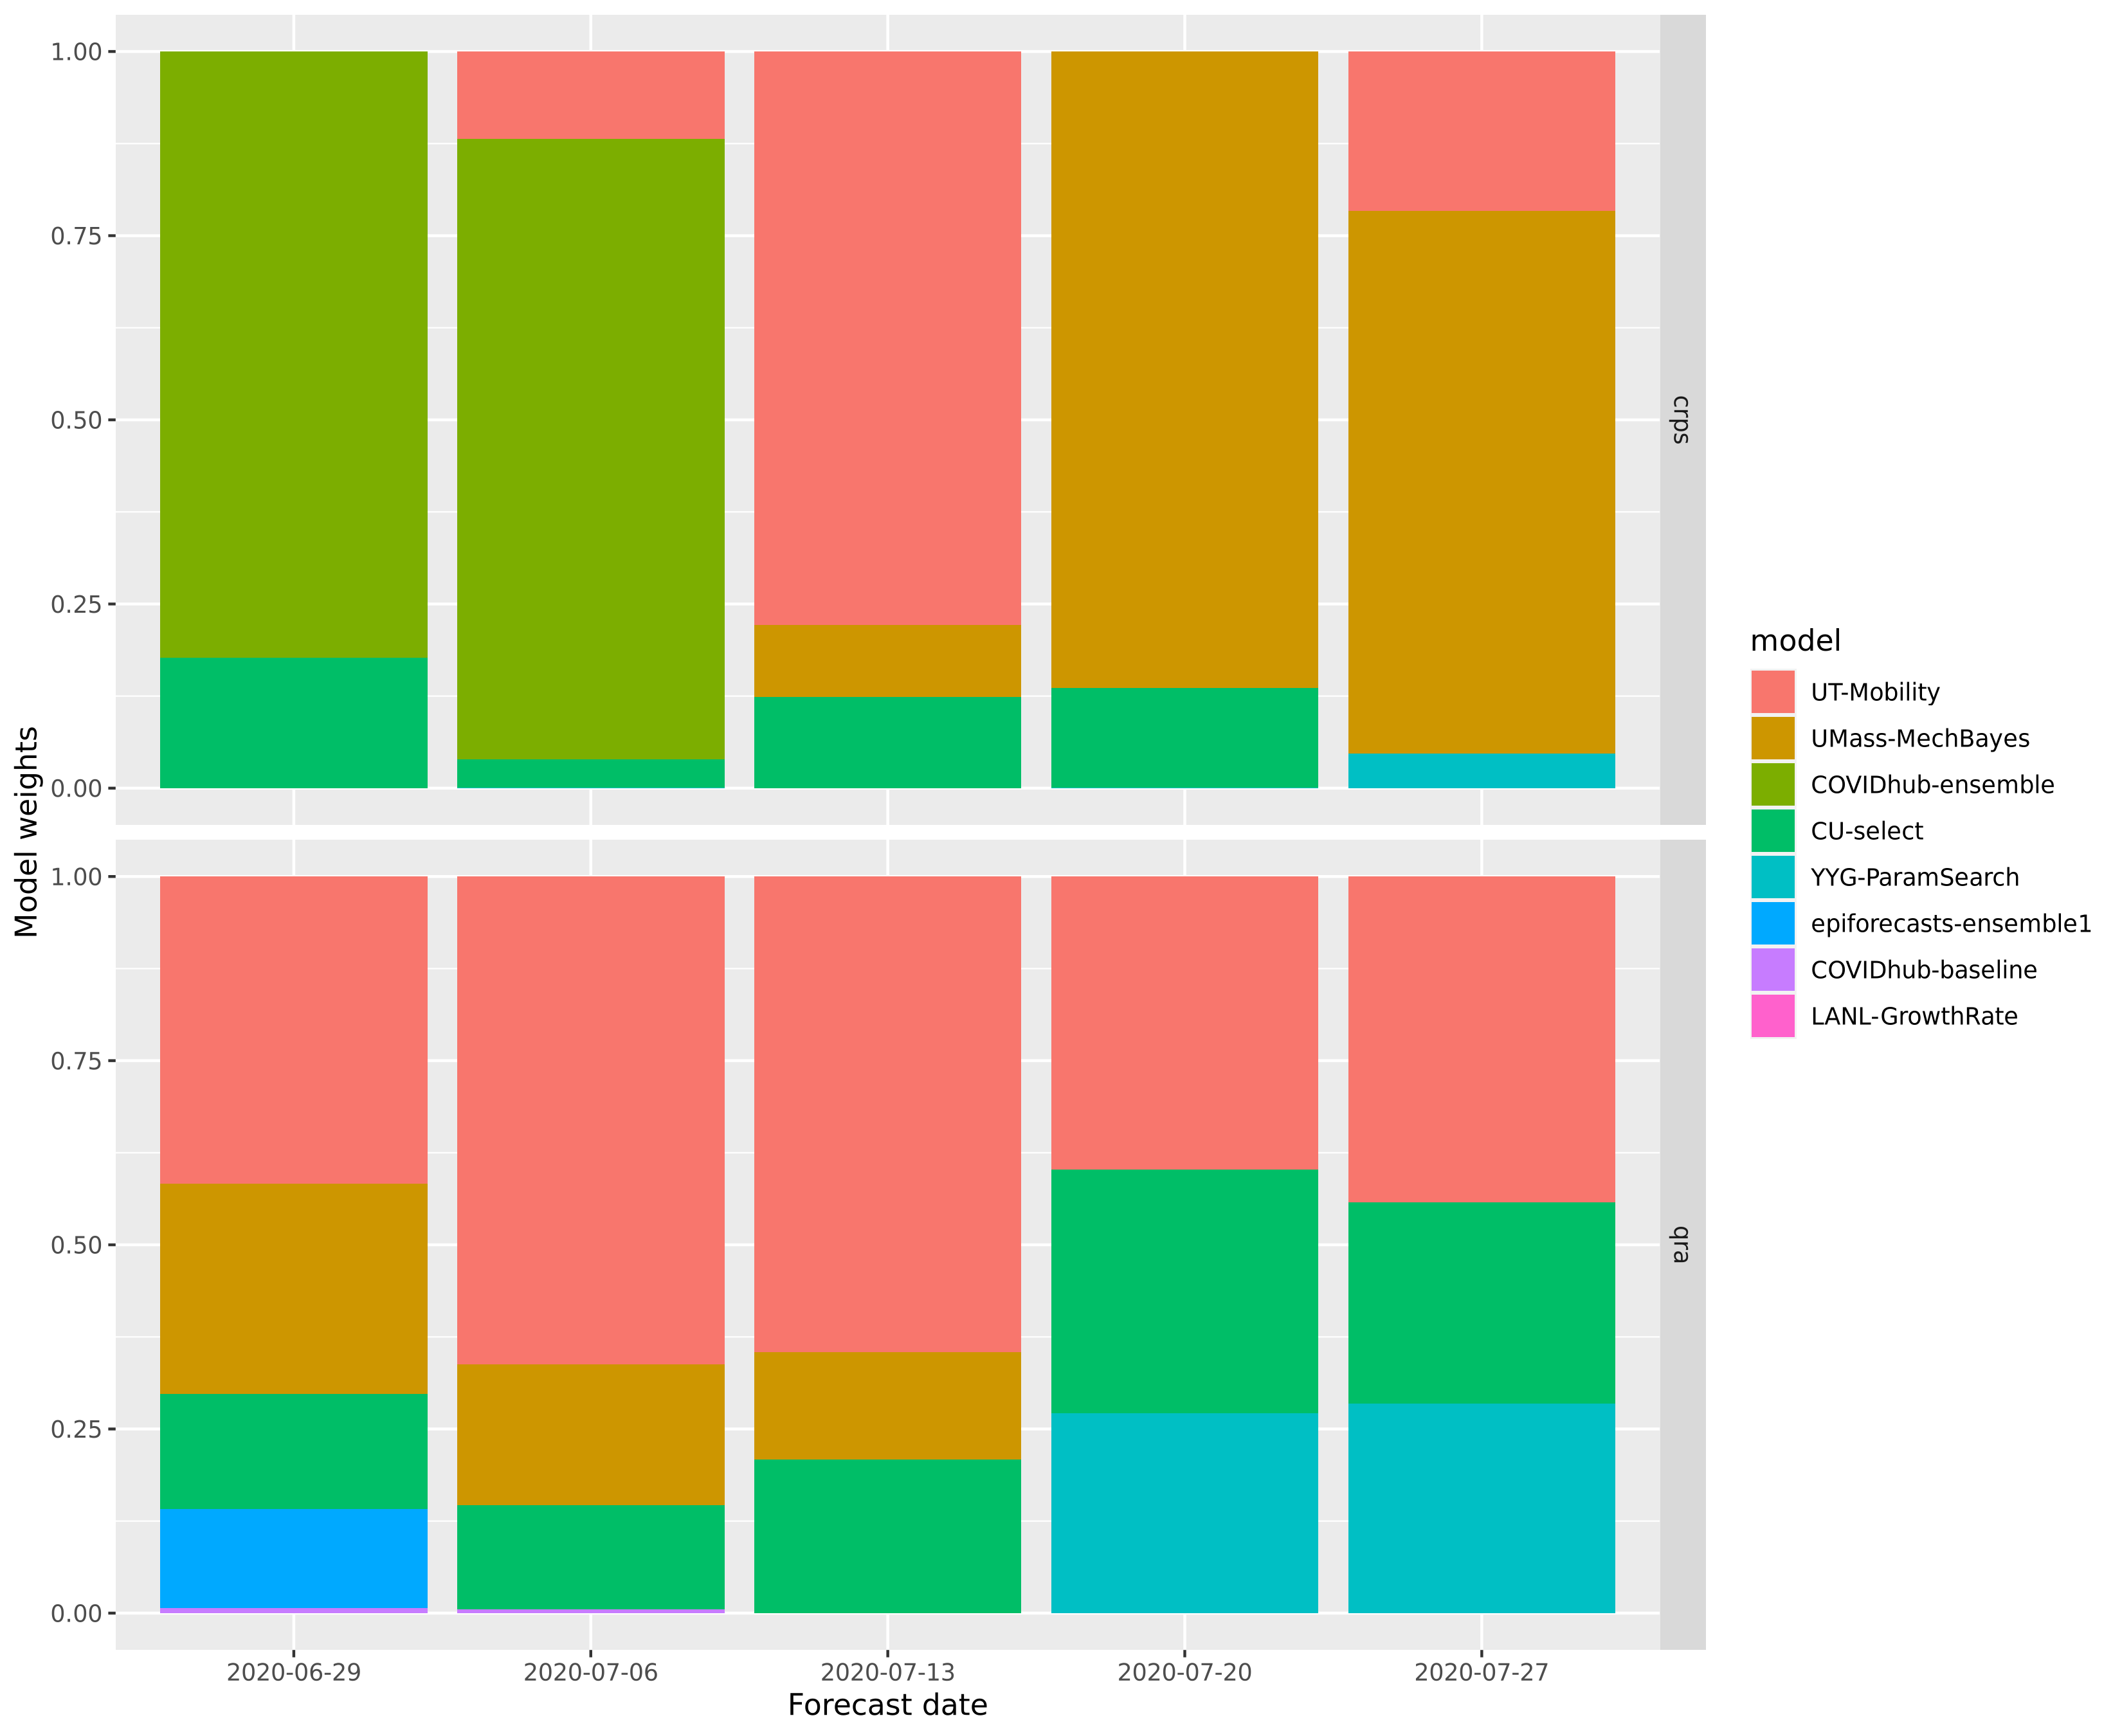
\includegraphics[width=1\linewidth]{../visualisation/chapter-5-results/weights-time} \caption{Weights given to the different models in the ensemble over time}\label{fig:weights-time}
\end{figure}

Figure \ref{fig:weights-vs-scores} shows the weights over time against the performance of the models. We can see that both ensembles prefer to include similar models. We can also see that model inclusion is not necessarily only determined by overall performance. For example, the CU-select and UT-Mobility model are included in both ensembles and seem to add something of value even though they are not among the top performers.

\begin{figure}
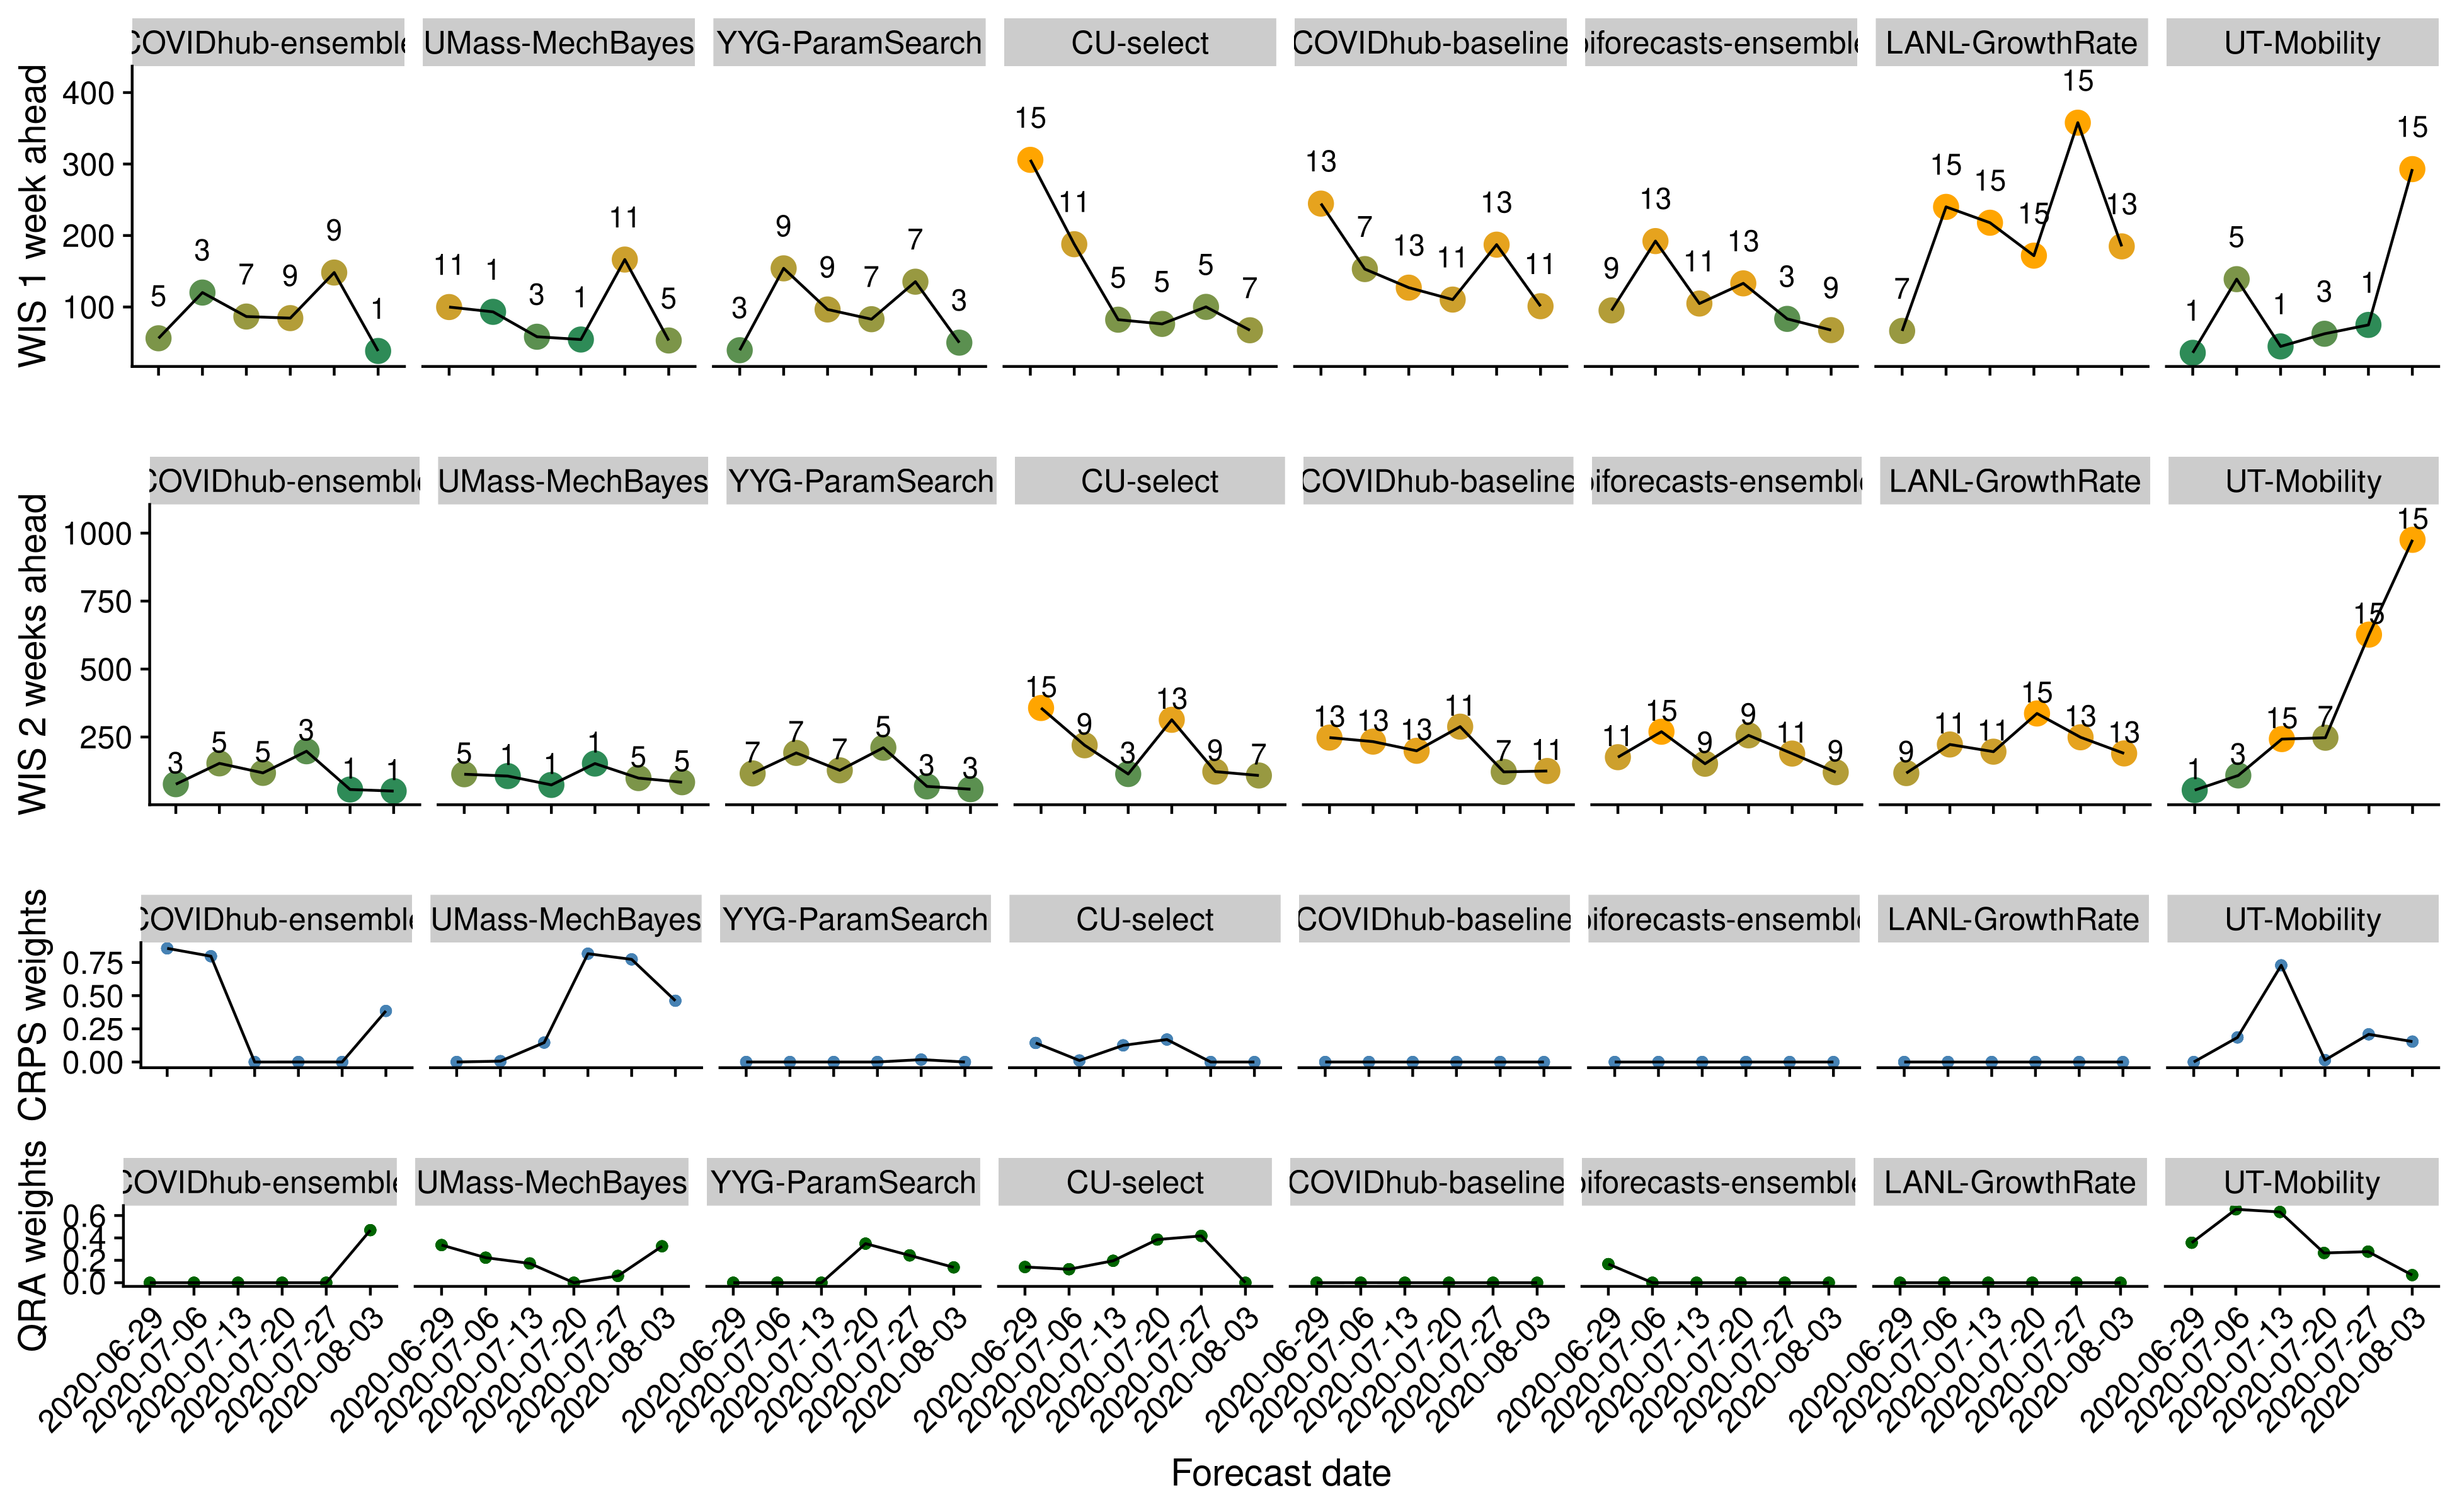
\includegraphics[width=1\linewidth]{../visualisation/chapter-5-results/weights-vs-wis} \caption{Weights given to the different models in the ensemble over time}\label{fig:weights-vs-scores}
\end{figure}

\hypertarget{other-ensemble-variants}{%
\section{Other ensemble variants}\label{other-ensemble-variants}}

The ensemble variants above are a sensible default, but are of course not the only possible ensemble combination. This section therefore explores different ensembles with different parameters. The default was run with otpimisation based on the two last forecasts. The qra ensembles were now run with one to four weeks of past forecasts and were therefore called qra-ensemble-1 to qra-ensemble-4. The default used previously corresponds to qra-ensemble-2. For the crps-ensemble, an additional choice was made, namely the horizon on which to optimise. In contrast to the \texttt{quantgen} package, \texttt{stackr} currently only supports one horizon. The second number in the crps-ensemble name therefore indicates the horizon for which the crps was optimised. The default model corresponds to crps-ensemble-2-2. We can see from a comparison with \ref{fig:coloured-summarised-scores} that aggregate scores for the crps-ensemble-2-2 model turn out slightly different. This can most certainly be explained by the fact that the crps-ensemble relies on random sampling.
Figure \ref{fig:ensemble-comparison} shows aggregate model performance for the different ensemble variants. No obvious picture emerges regarding the superiority of either qra or crps ensembles. There is, however, a couple of interesting patterns to observe. Firstly, crps-ensembles optimised only on one-week-ahead forecast horizon tend to do worst, while those optimised on three and especially two weeks do best. For the crps ensemble it seems that the forecast horizon matters more than the number of past forecasts included in the weighting. This is somewhat surprising given that qra-ensemble-1 is among the top performers. If we only ever include the past forecast, this of course implies that weighting can only be done on one-week-ahead forecasts. Normally, we would therefore expect the qra-ensemble-1 to perform similarly to crps-ensemble-1-1. We can also see that the qra-ensemble-4 and qra-ensemble-1 are top performers, while qra-ensemble-3 and qra-ensemble-2 are not. This casts doubt whether there is a clear best choice of the number of past observations to include. Additional analysis could be conducted by including arbitrary combinations of horizons in the qra optimisation instead of simply all available horizons. We also see that qra ensemble tend to overpredict, while crps ensembles tend to underpredict. This, however, may also be an artifact of the model aggregation process in which a gamma distribution gets fit to predictive quantiles.

\begin{figure}
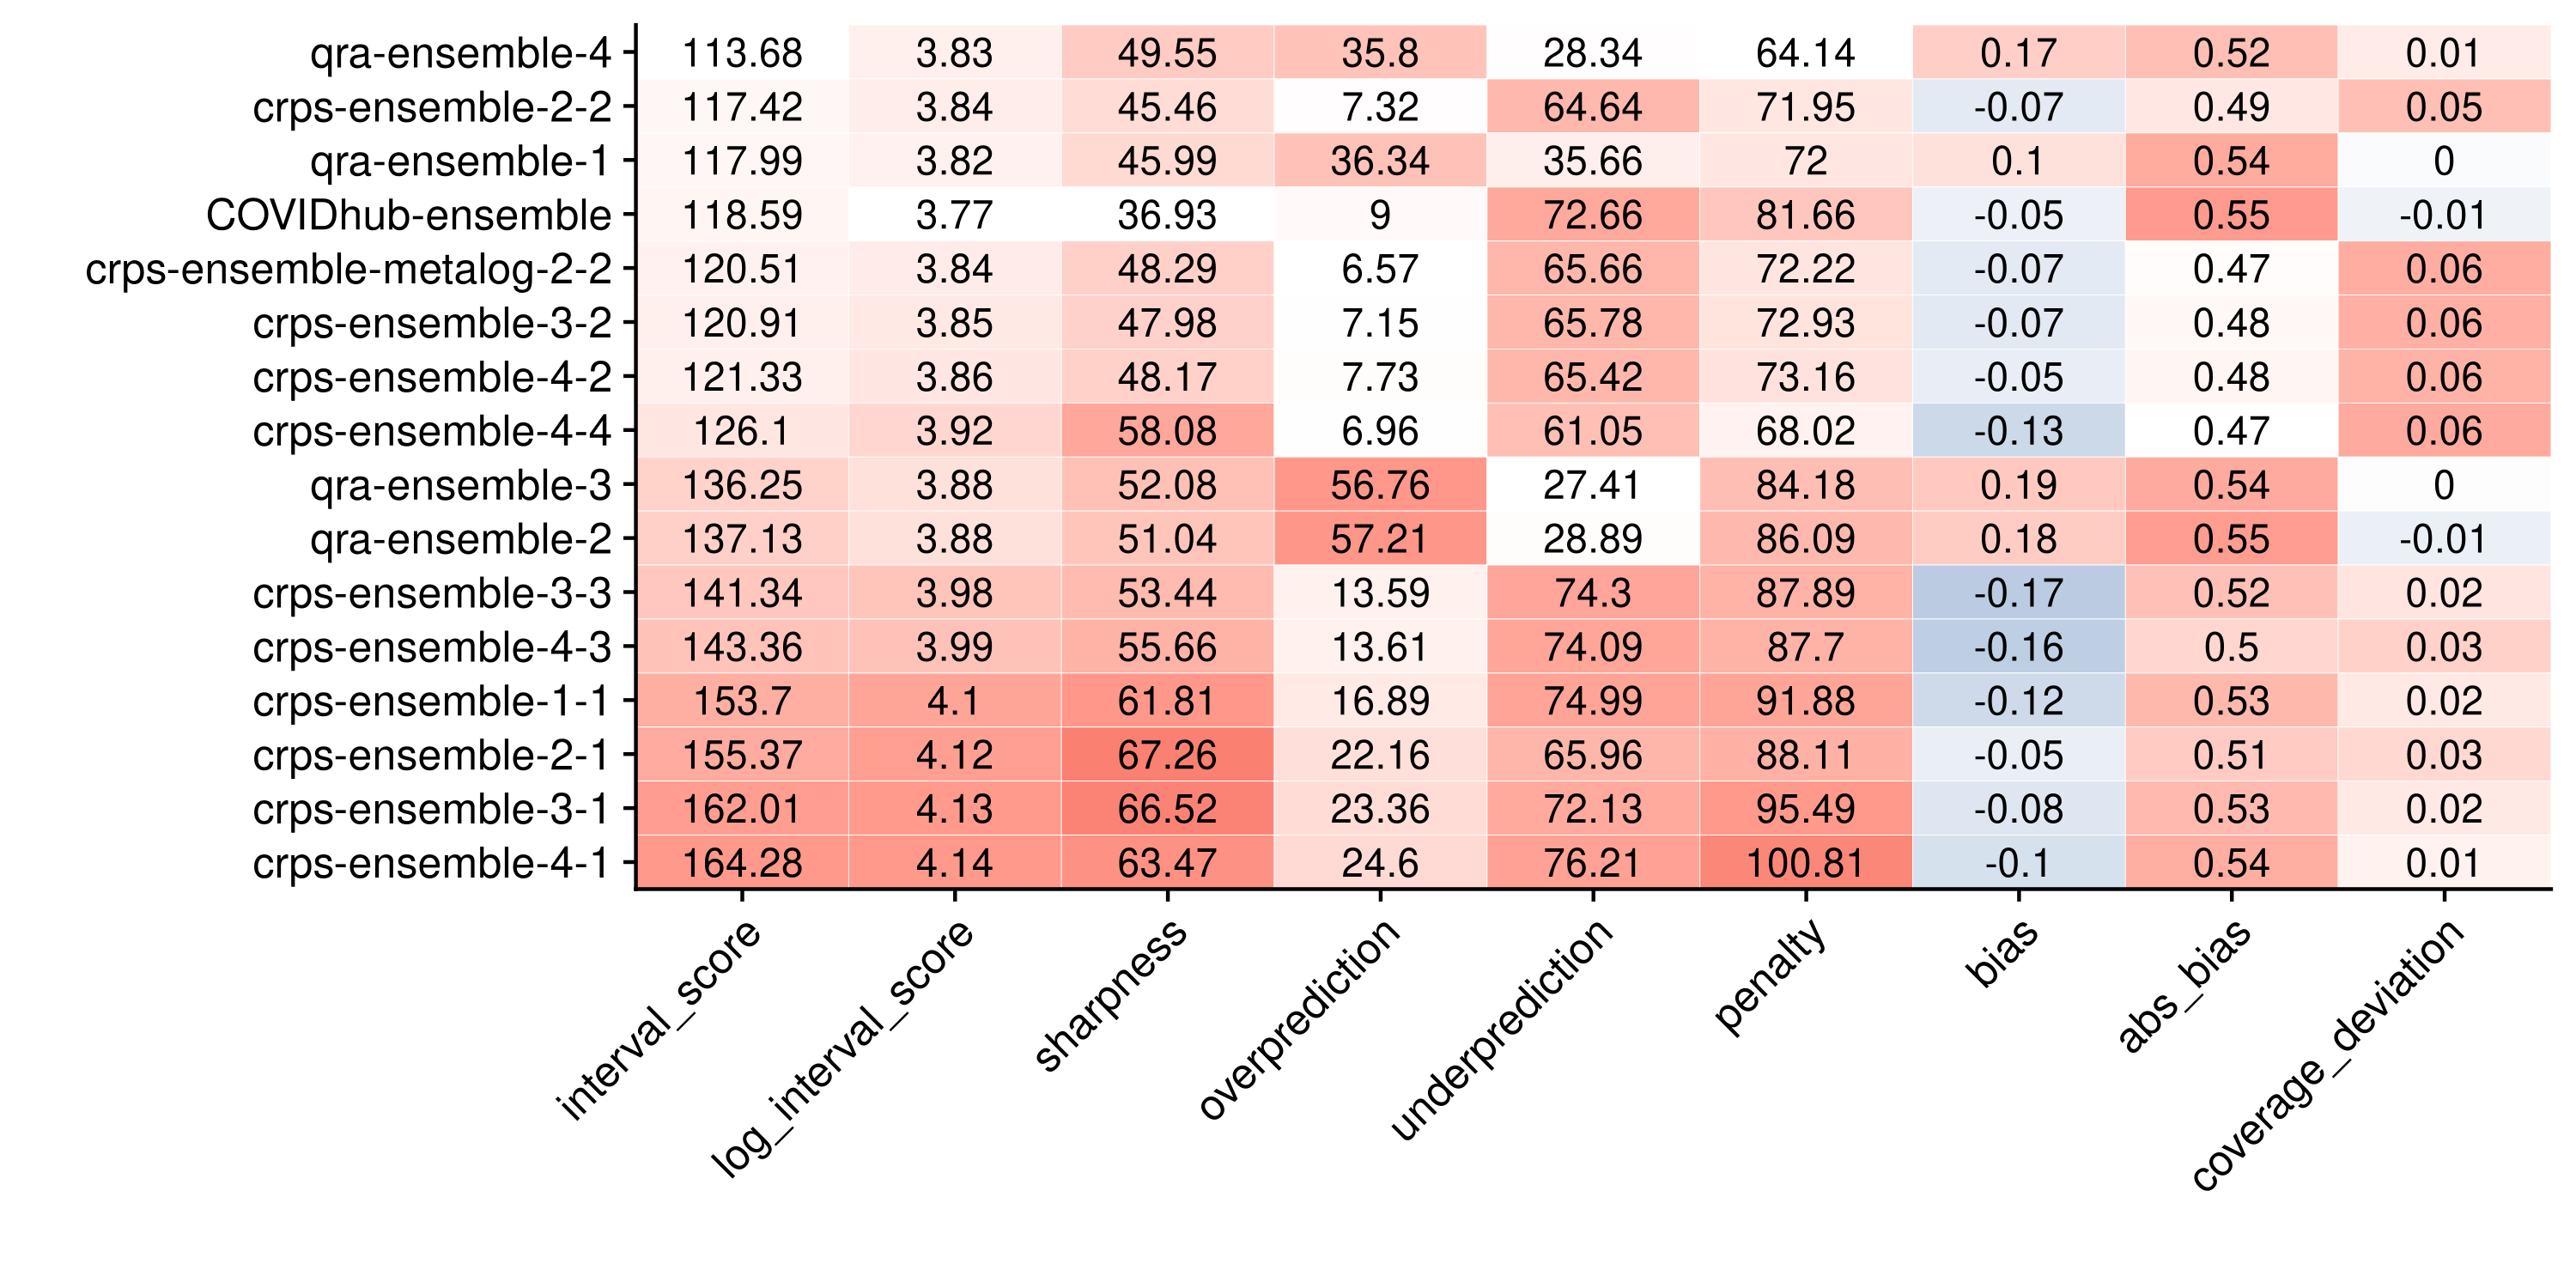
\includegraphics[width=1\linewidth]{../visualisation/chapter-5-results/ensembles/scenario-baseline/coloured-summarised-scores} \caption{Weights given to the different models in the ensemble over time}\label{fig:ensemble-comparison}
\end{figure}

\begin{table}

\caption{\label{tab:regression-ensemble}Mixed model regression of the log weighted interval score on model (fixed), state, and forecast date (both random)}
\centering
\resizebox{\linewidth}{!}{
\begin{tabular}[t]{lrrrrr}
\toprule
  & Estimate & Std. Error & df & t value & Pr(>|t|)\\
\midrule
(Intercept) & 3.8078748 & 0.3181880 & 13.94955 & 11.9673741 & 0.0000000\\
modelcrps-ensemble-4-1 & 0.3180304 & 0.0532436 & 4154.98761 & 5.9731245 & 0.0000000\\
modelcrps-ensemble-3-1 & 0.3142822 & 0.0532436 & 4154.98761 & 5.9027272 & 0.0000000\\
modelcrps-ensemble-2-1 & 0.2963384 & 0.0532436 & 4154.98761 & 5.5657133 & 0.0000000\\
modelcrps-ensemble-1-1 & 0.2758819 & 0.0532436 & 4154.98761 & 5.1815081 & 0.0000002\\
\addlinespace
modelcrps-ensemble-4-3 & 0.1709521 & 0.0532436 & 4154.98761 & 3.2107559 & 0.0013339\\
modelcrps-ensemble-3-3 & 0.1602553 & 0.0532436 & 4154.98761 & 3.0098525 & 0.0026294\\
modelcrps-ensemble-4-4 & 0.0966253 & 0.0532436 & 4154.98761 & 1.8147787 & 0.0696300\\
modelqra-ensemble-2 & 0.0603194 & 0.0532436 & 4154.98761 & 1.1328961 & 0.2573233\\
modelqra-ensemble-3 & 0.0599485 & 0.0532436 & 4154.98761 & 1.1259294 & 0.2602605\\
\addlinespace
modelcrps-ensemble-4-2 & 0.0396256 & 0.0532436 & 4154.98761 & 0.7442321 & 0.4567782\\
modelcrps-ensemble-3-2 & 0.0318226 & 0.0532436 & 4154.98761 & 0.5976795 & 0.5500864\\
modelcrps-ensemble-2-2 & 0.0152883 & 0.0532436 & 4154.98761 & 0.2871387 & 0.7740204\\
modelqra-ensemble-4 & 0.0052770 & 0.0532436 & 4154.98761 & 0.0991108 & 0.9210551\\
\bottomrule
\end{tabular}}
\end{table}

INTERESTING: WEIGHTS OVER TIME

ADD TO INTERPRETATION: The second thing to keep in mind is that the crps-ensemble implementation in this thesis entails fitting a gamma distribution to the set of predictive quantiles which is bound to lose some precision. It is therefore expected to the see the crps-ensemble perform worse and therefore rather surprising that it keeps up in performance with the other ensembles.

\hypertarget{sensitivity-analysis}{%
\section{Sensitivity analysis}\label{sensitivity-analysis}}

In order to test the validity and robustness of the results obtained, this section presents a small validity analysis. This analysis could of course be expanded greatly.

Instead of looking at the whole time window, the three latest dates were successively removed. Figure \ref{fig:senitivity} shows the summarised scores for all models in the four different scenarios. We can see XXX.

\begin{figure}
\includegraphics[width=0.5\linewidth]{../visualisation/chapter-5-results/scenario-baseline/coloured-summarised-scores} 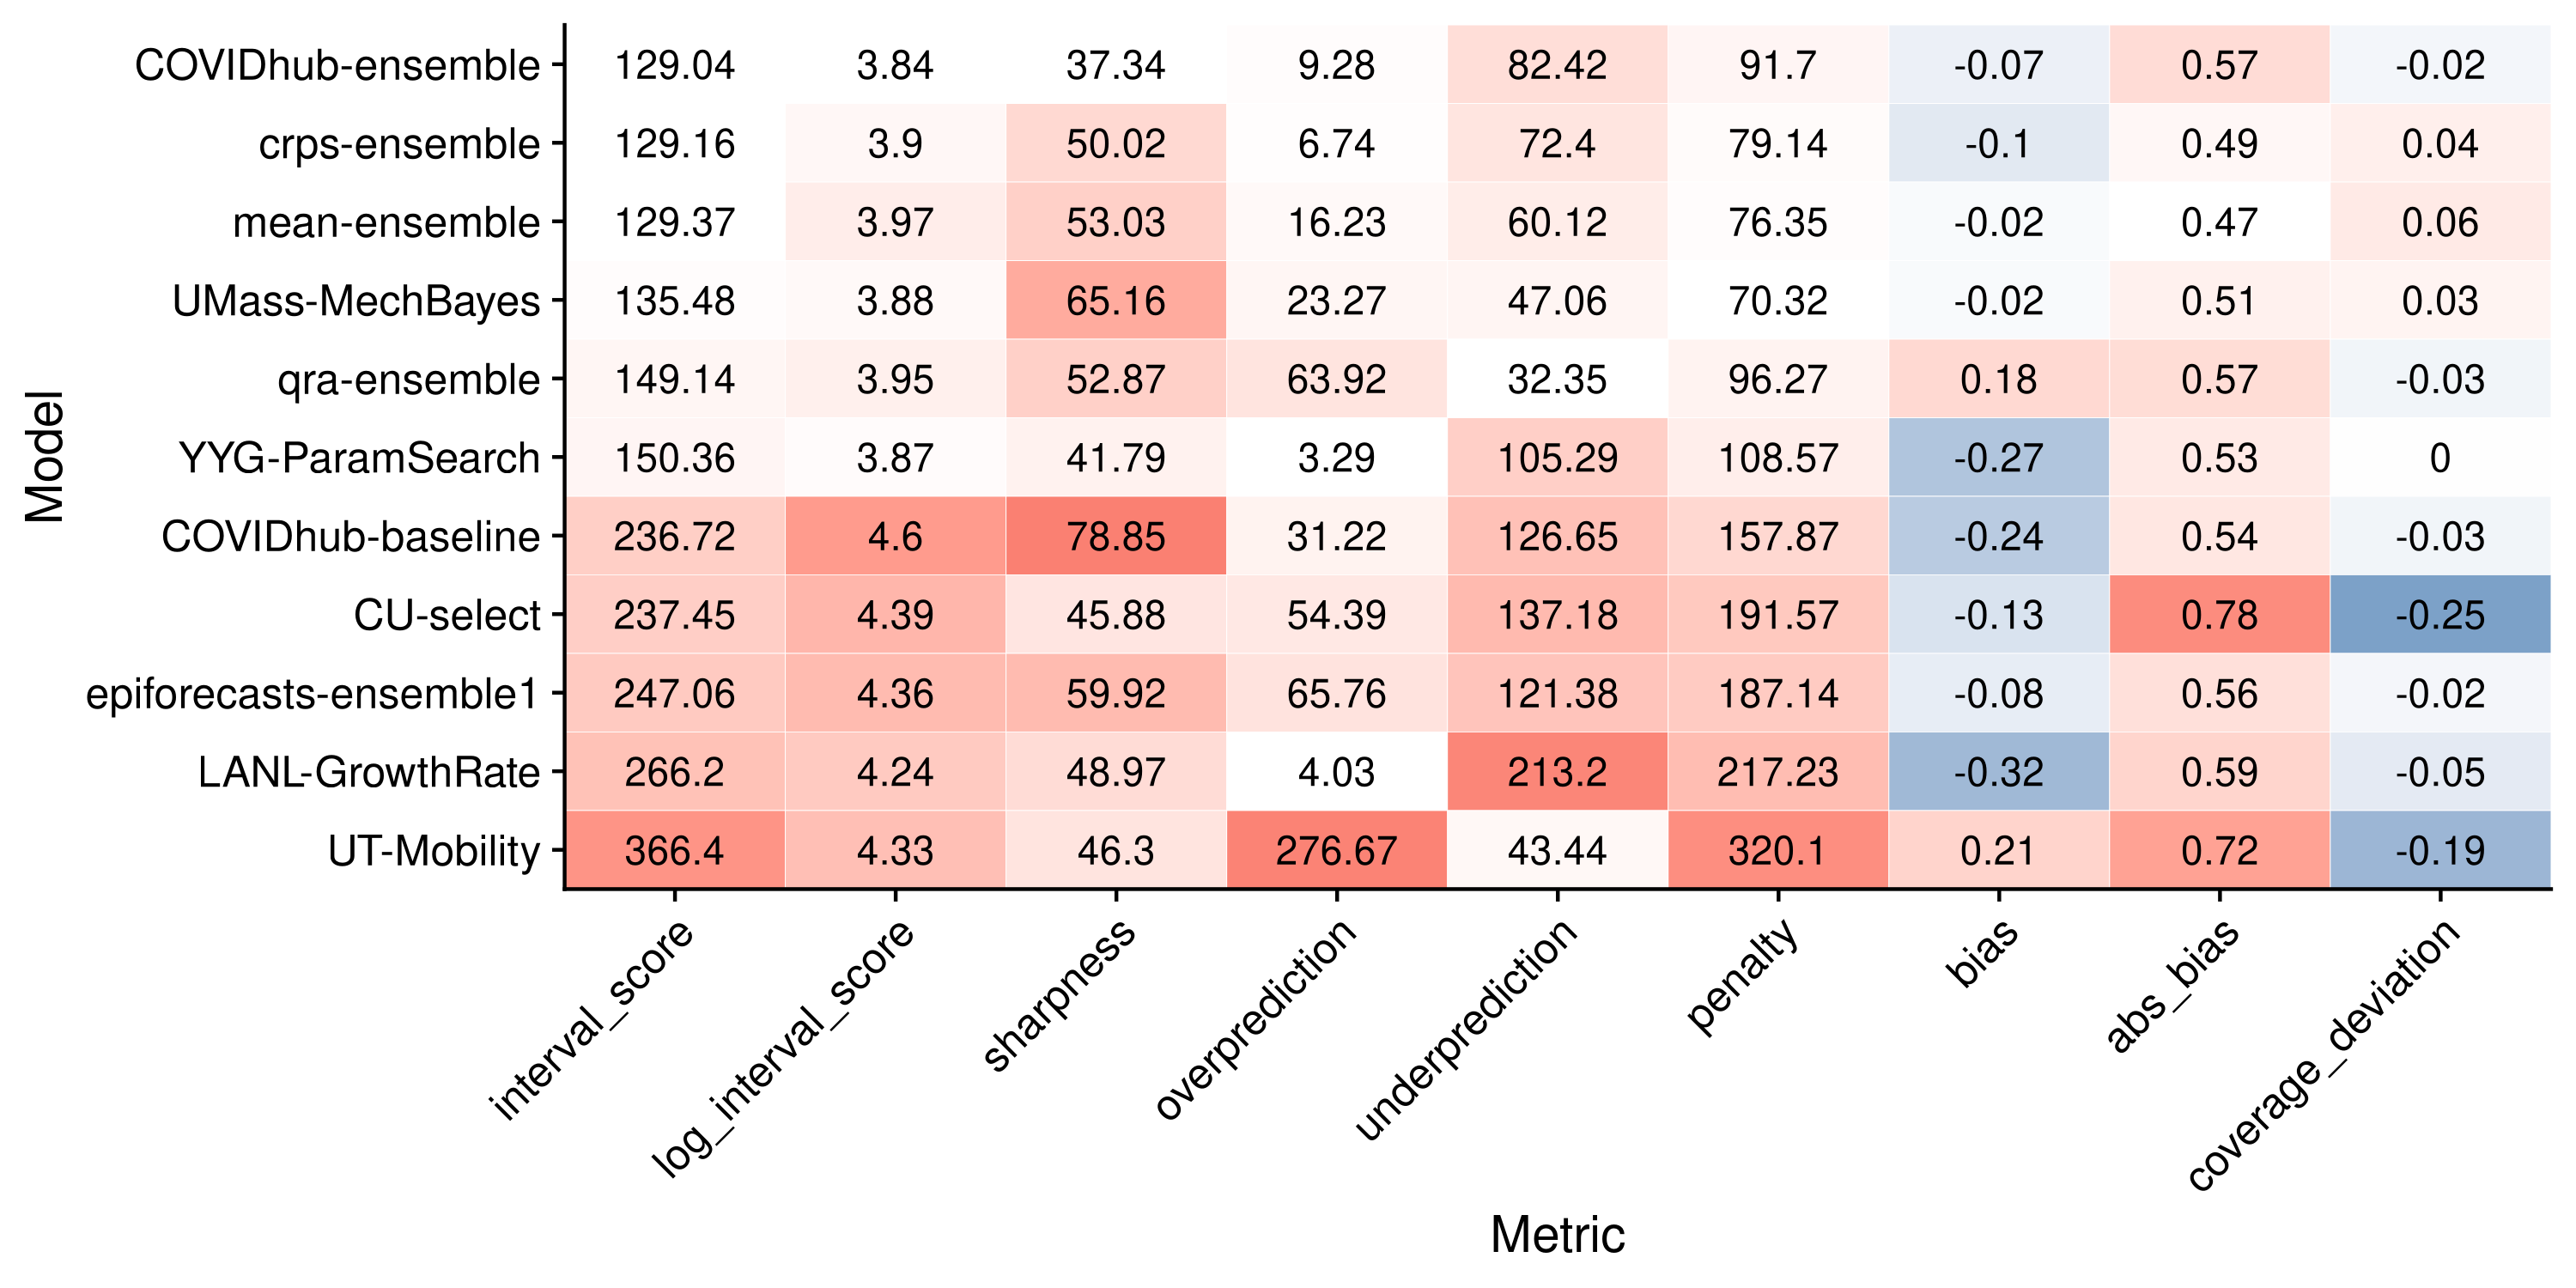
\includegraphics[width=0.5\linewidth]{../visualisation/chapter-5-results/scenario-1/coloured-summarised-scores} \includegraphics[width=0.5\linewidth]{../visualisation/chapter-5-results/scenario-2/coloured-summarised-scores} 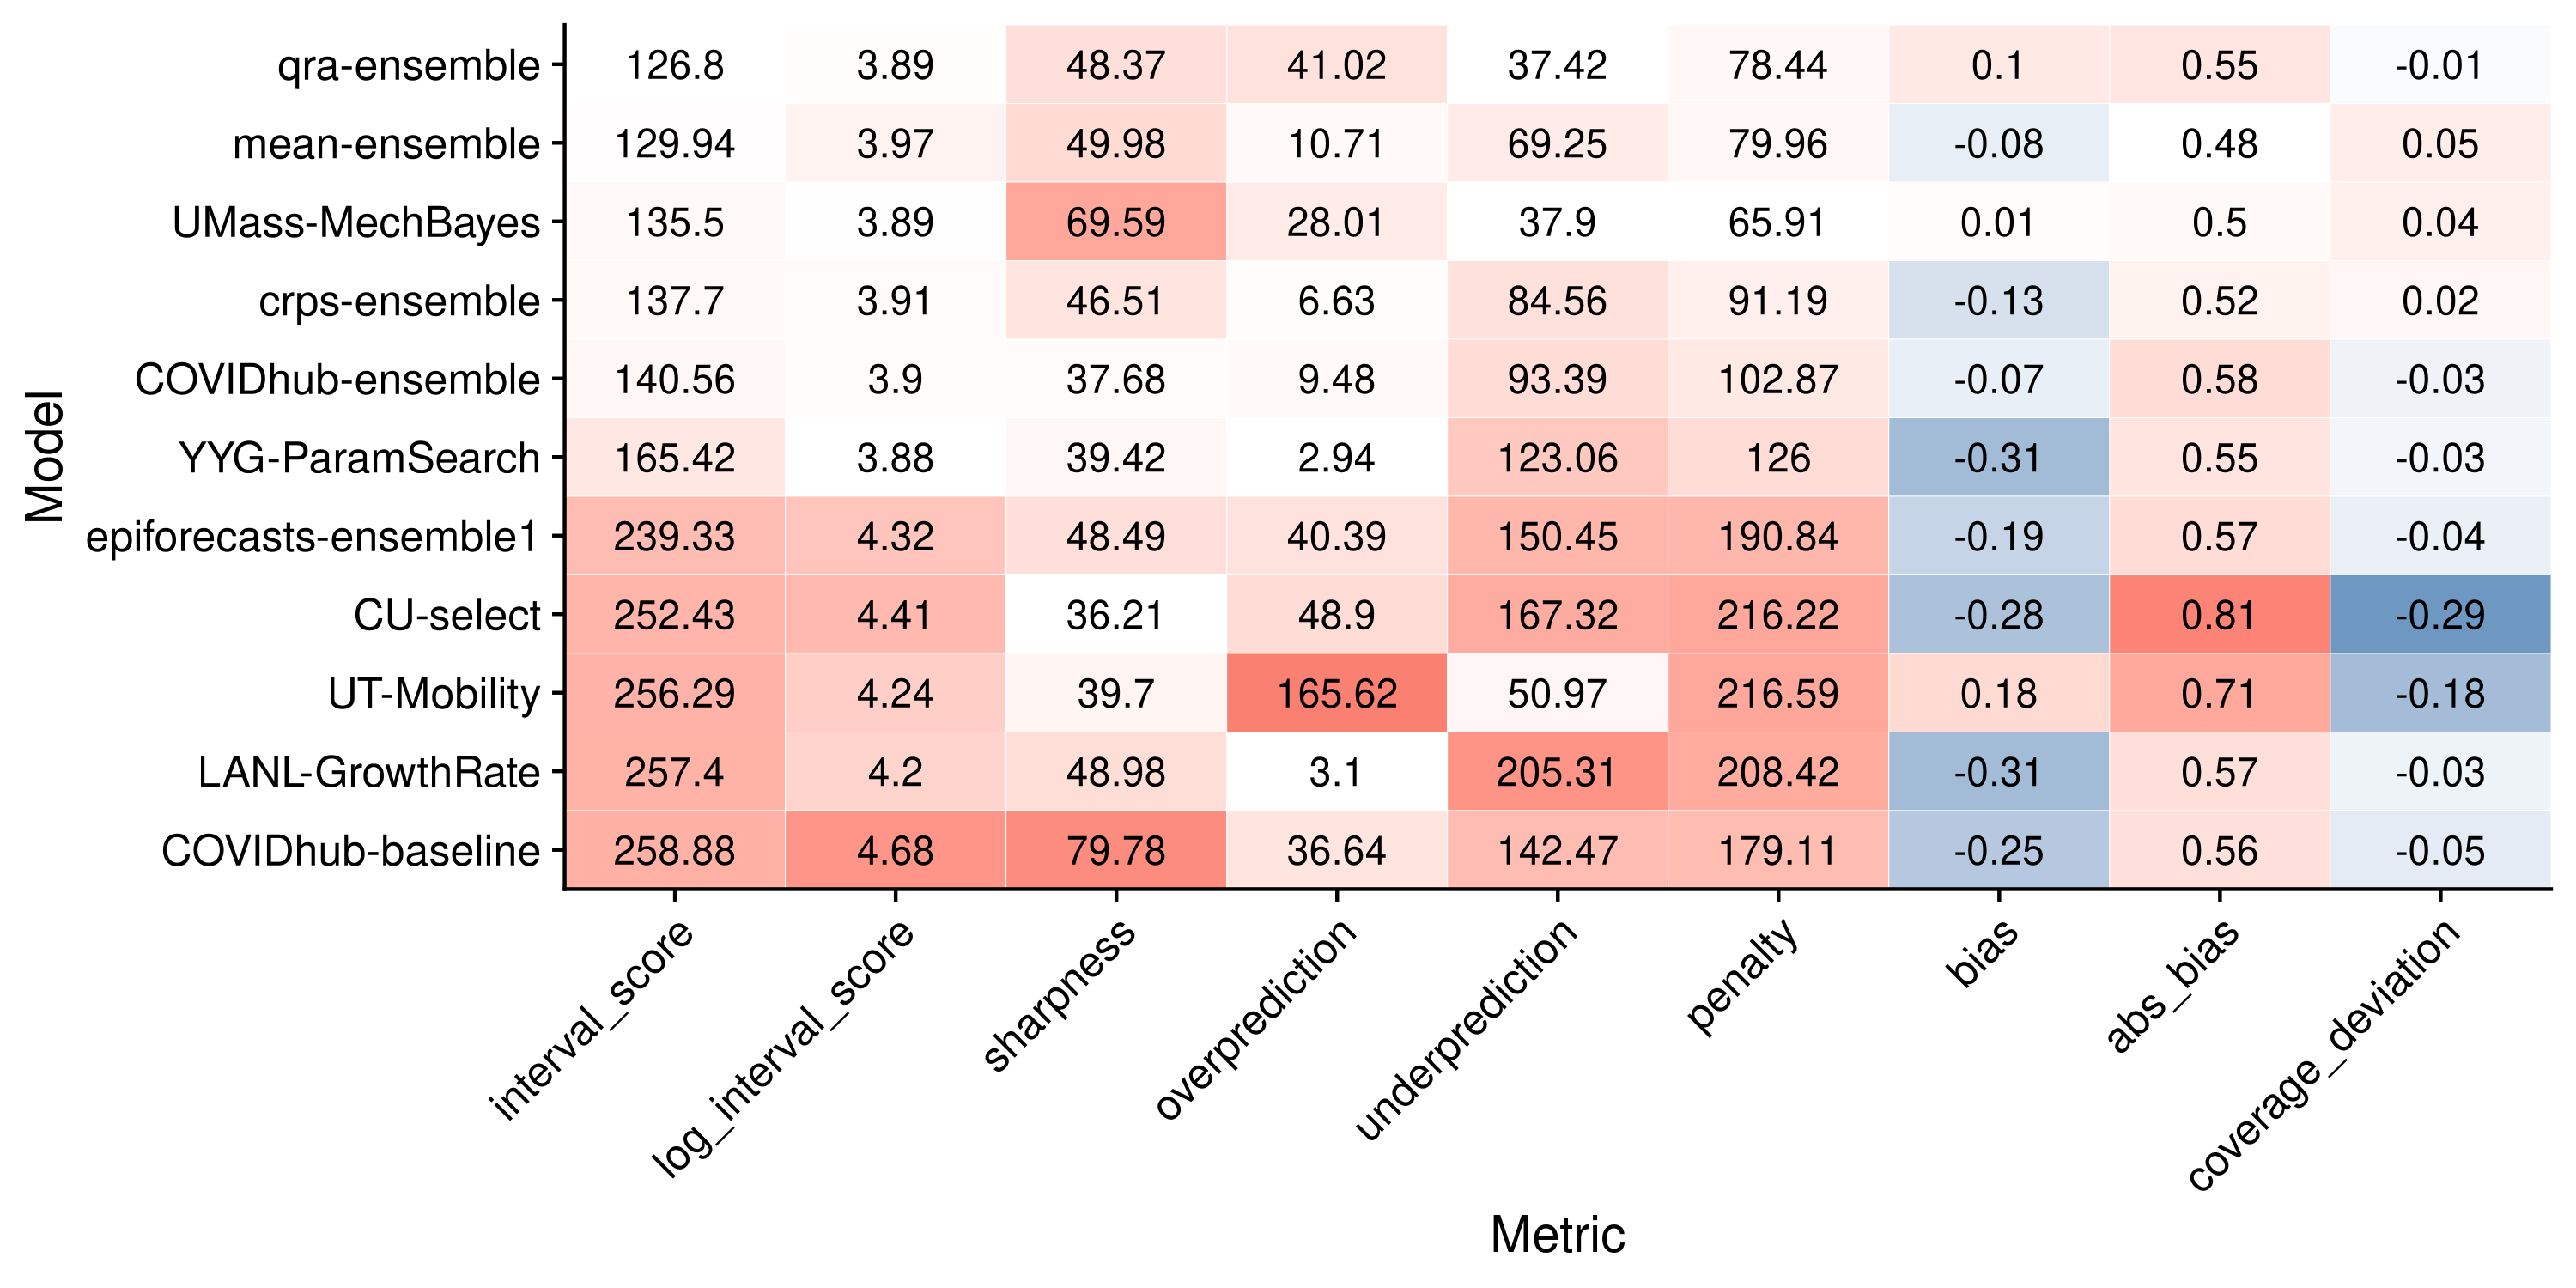
\includegraphics[width=0.5\linewidth]{../visualisation/chapter-5-results/scenario-3/coloured-summarised-scores} \caption{Weights given to the different models in the ensemble over time}\label{fig:senitivity}
\end{figure}

The same analysis is of course also interesting for the ensemble variants. Figure \ref{fig:senitivity} therefore shows aggregated scores for all ensemble variants for the four different scenarios. REWORK INTERPRETATION. qra-ensemble-4 stays at the top consistently, it seems like qra is slightly outperforming crps. It still seems like crps-ensemble horizon 2 is best.

\begin{figure}
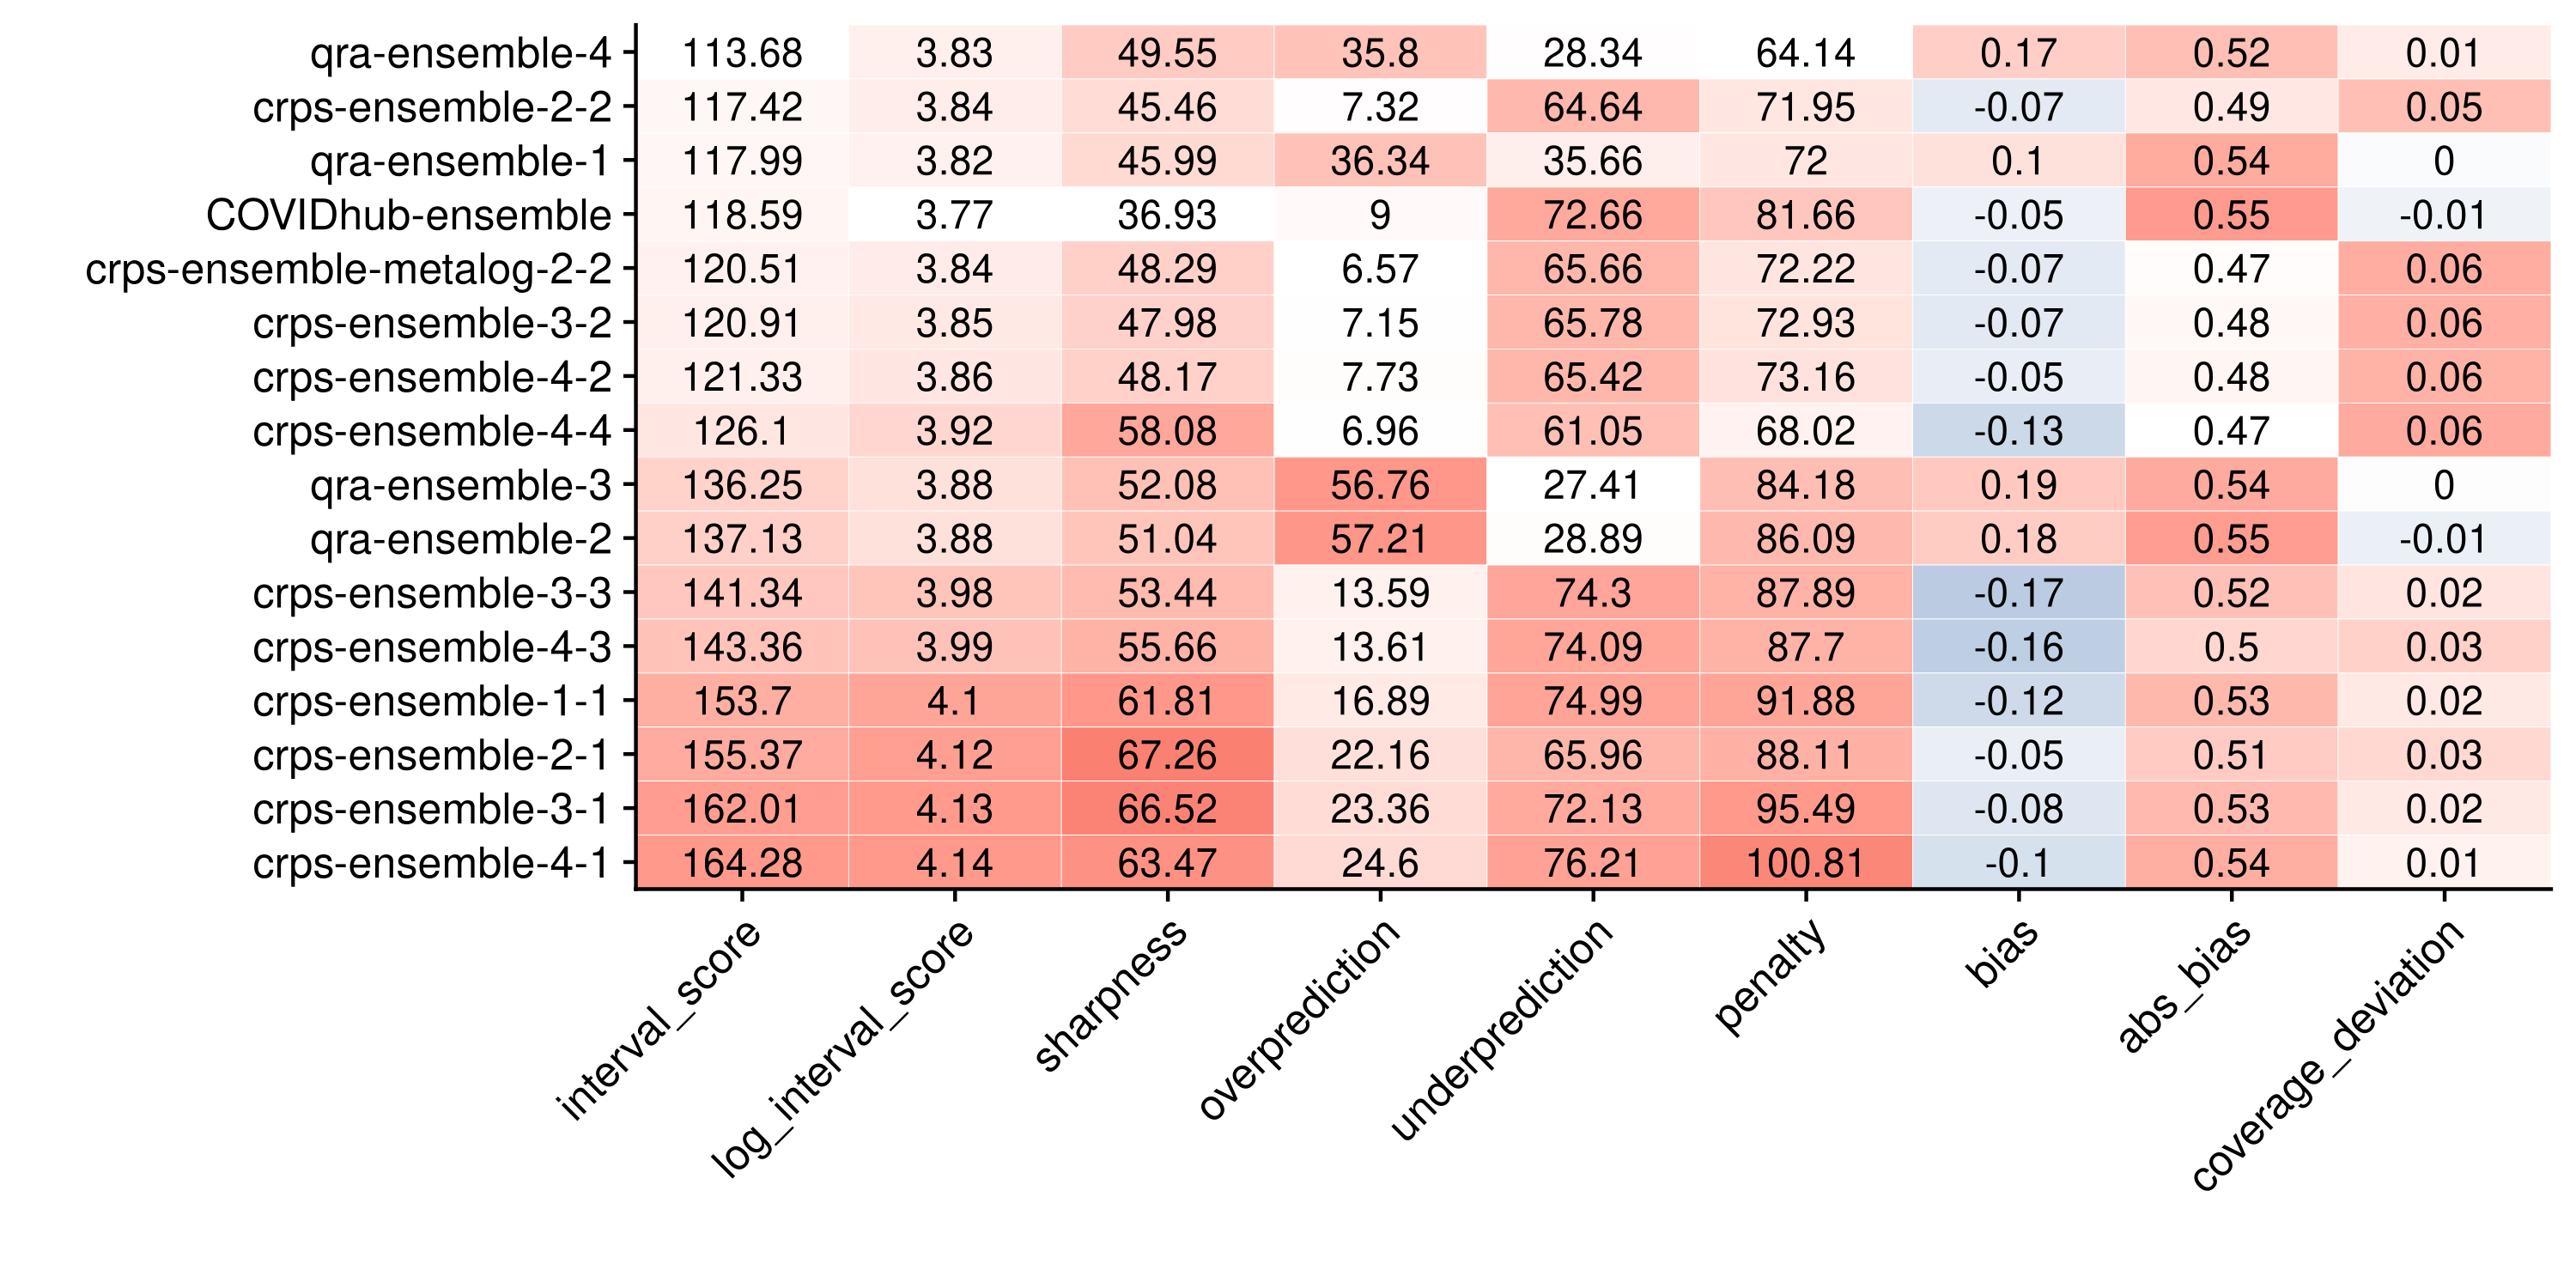
\includegraphics[width=0.5\linewidth]{../visualisation/chapter-5-results/ensembles/scenario-baseline/coloured-summarised-scores} 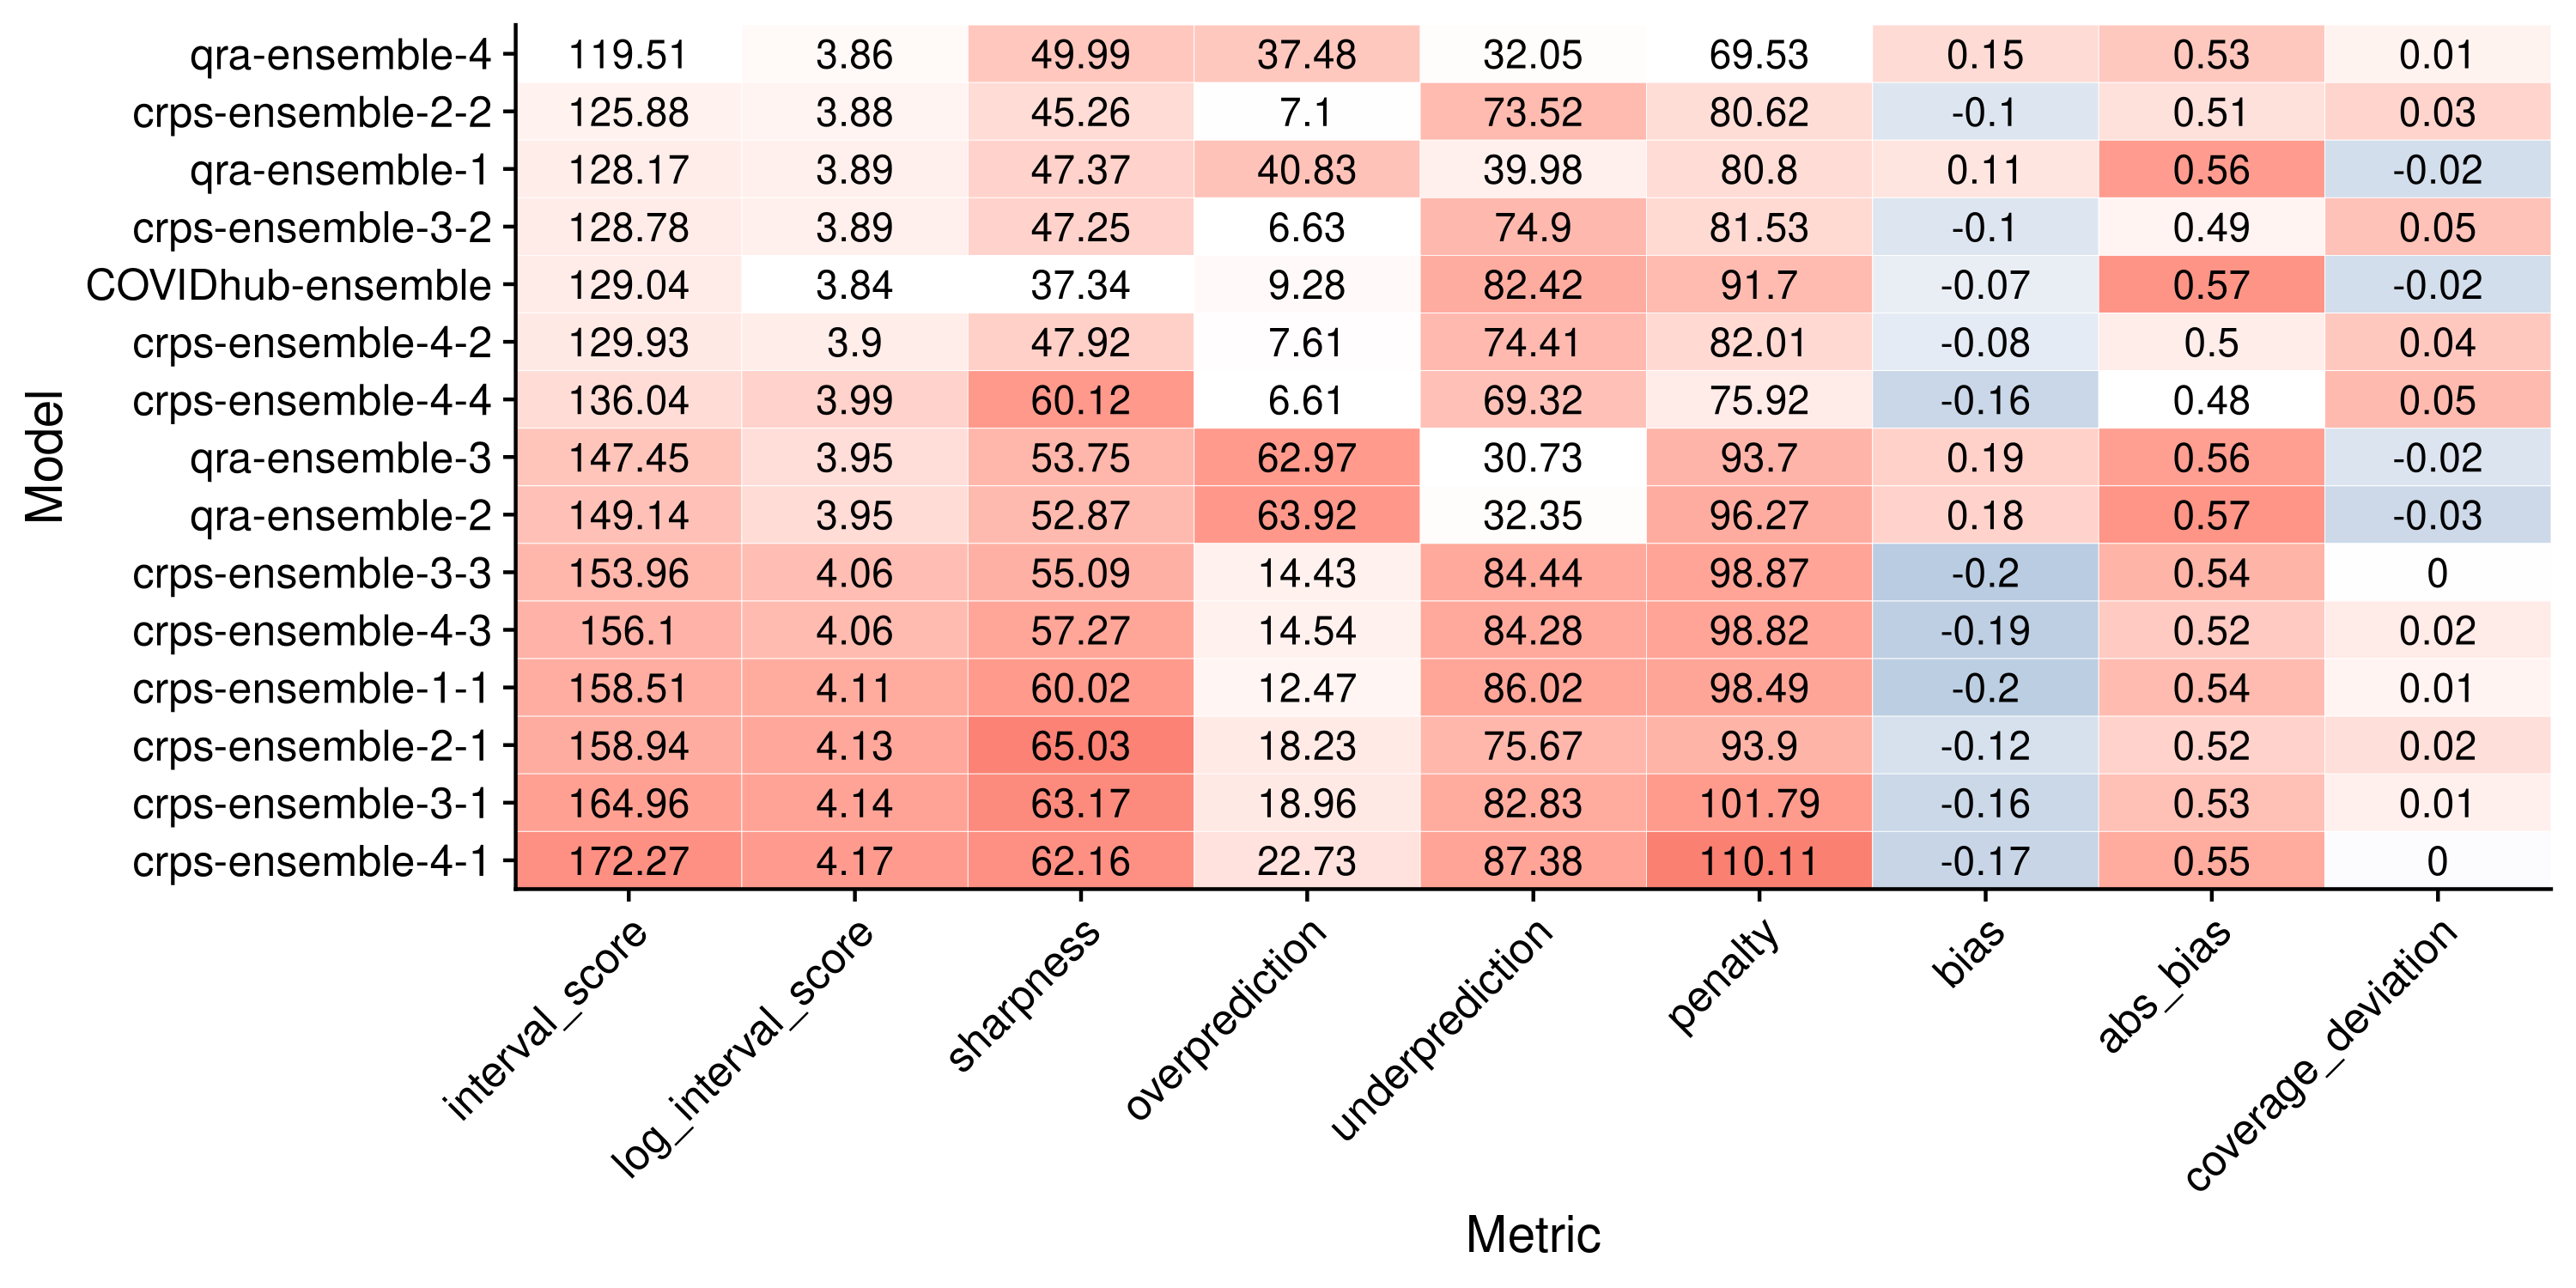
\includegraphics[width=0.5\linewidth]{../visualisation/chapter-5-results/ensembles/scenario-1/coloured-summarised-scores} 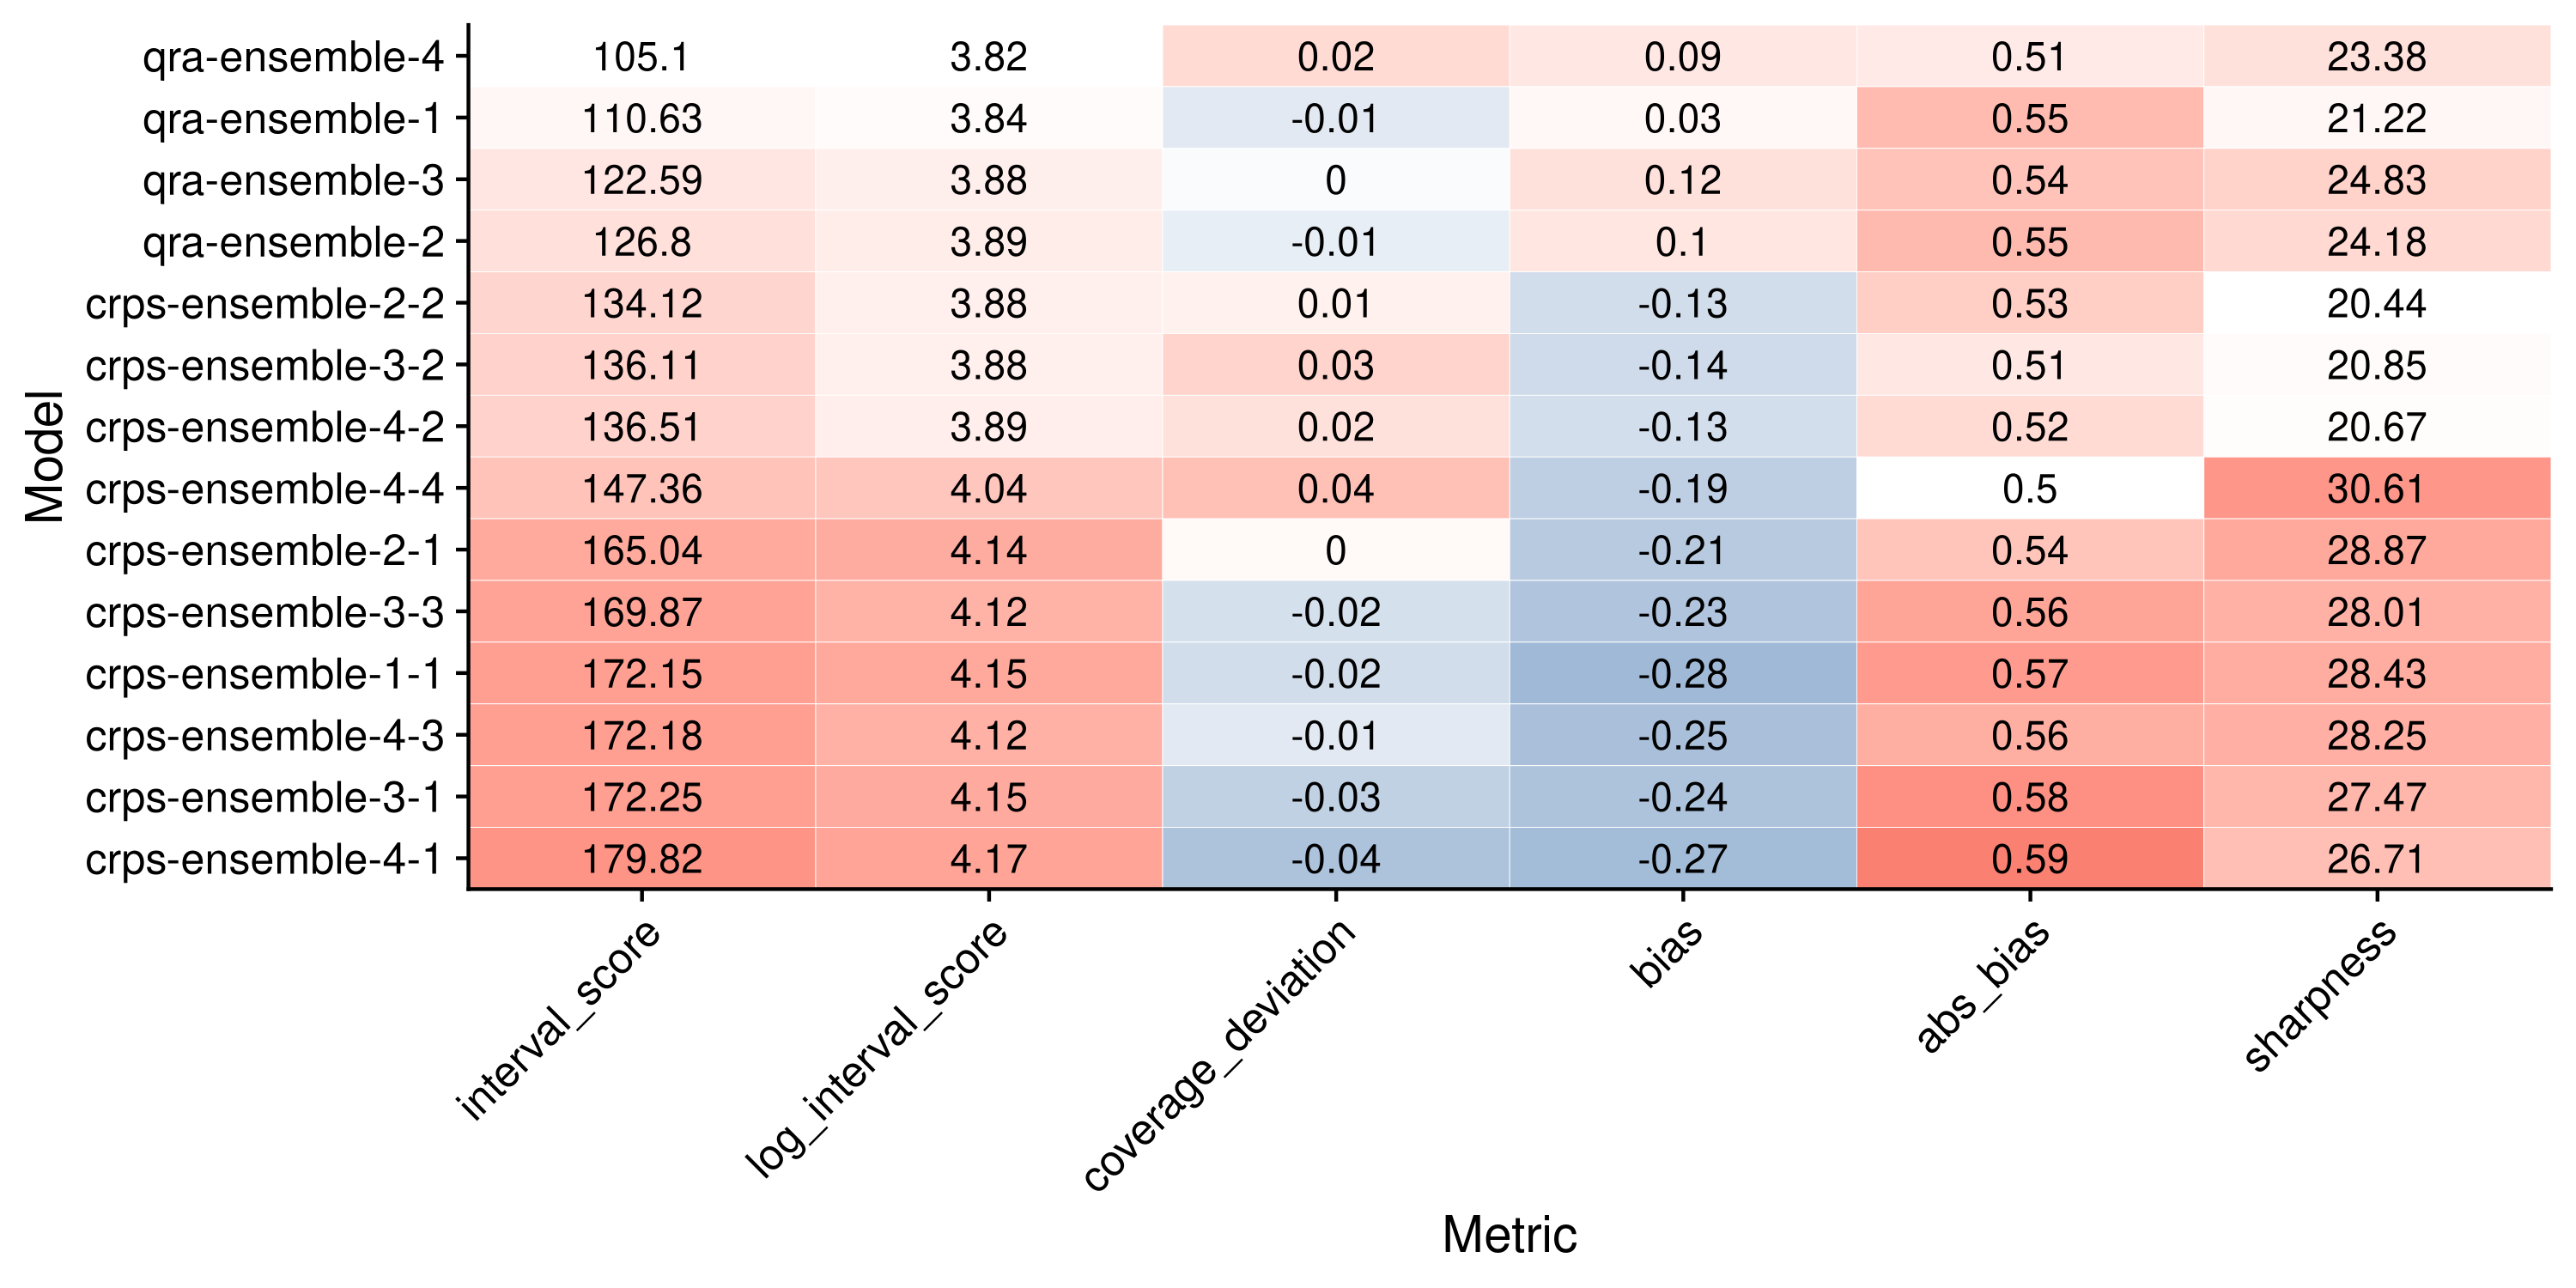
\includegraphics[width=0.5\linewidth]{../visualisation/chapter-5-results/ensembles/scenario-2/coloured-summarised-scores} 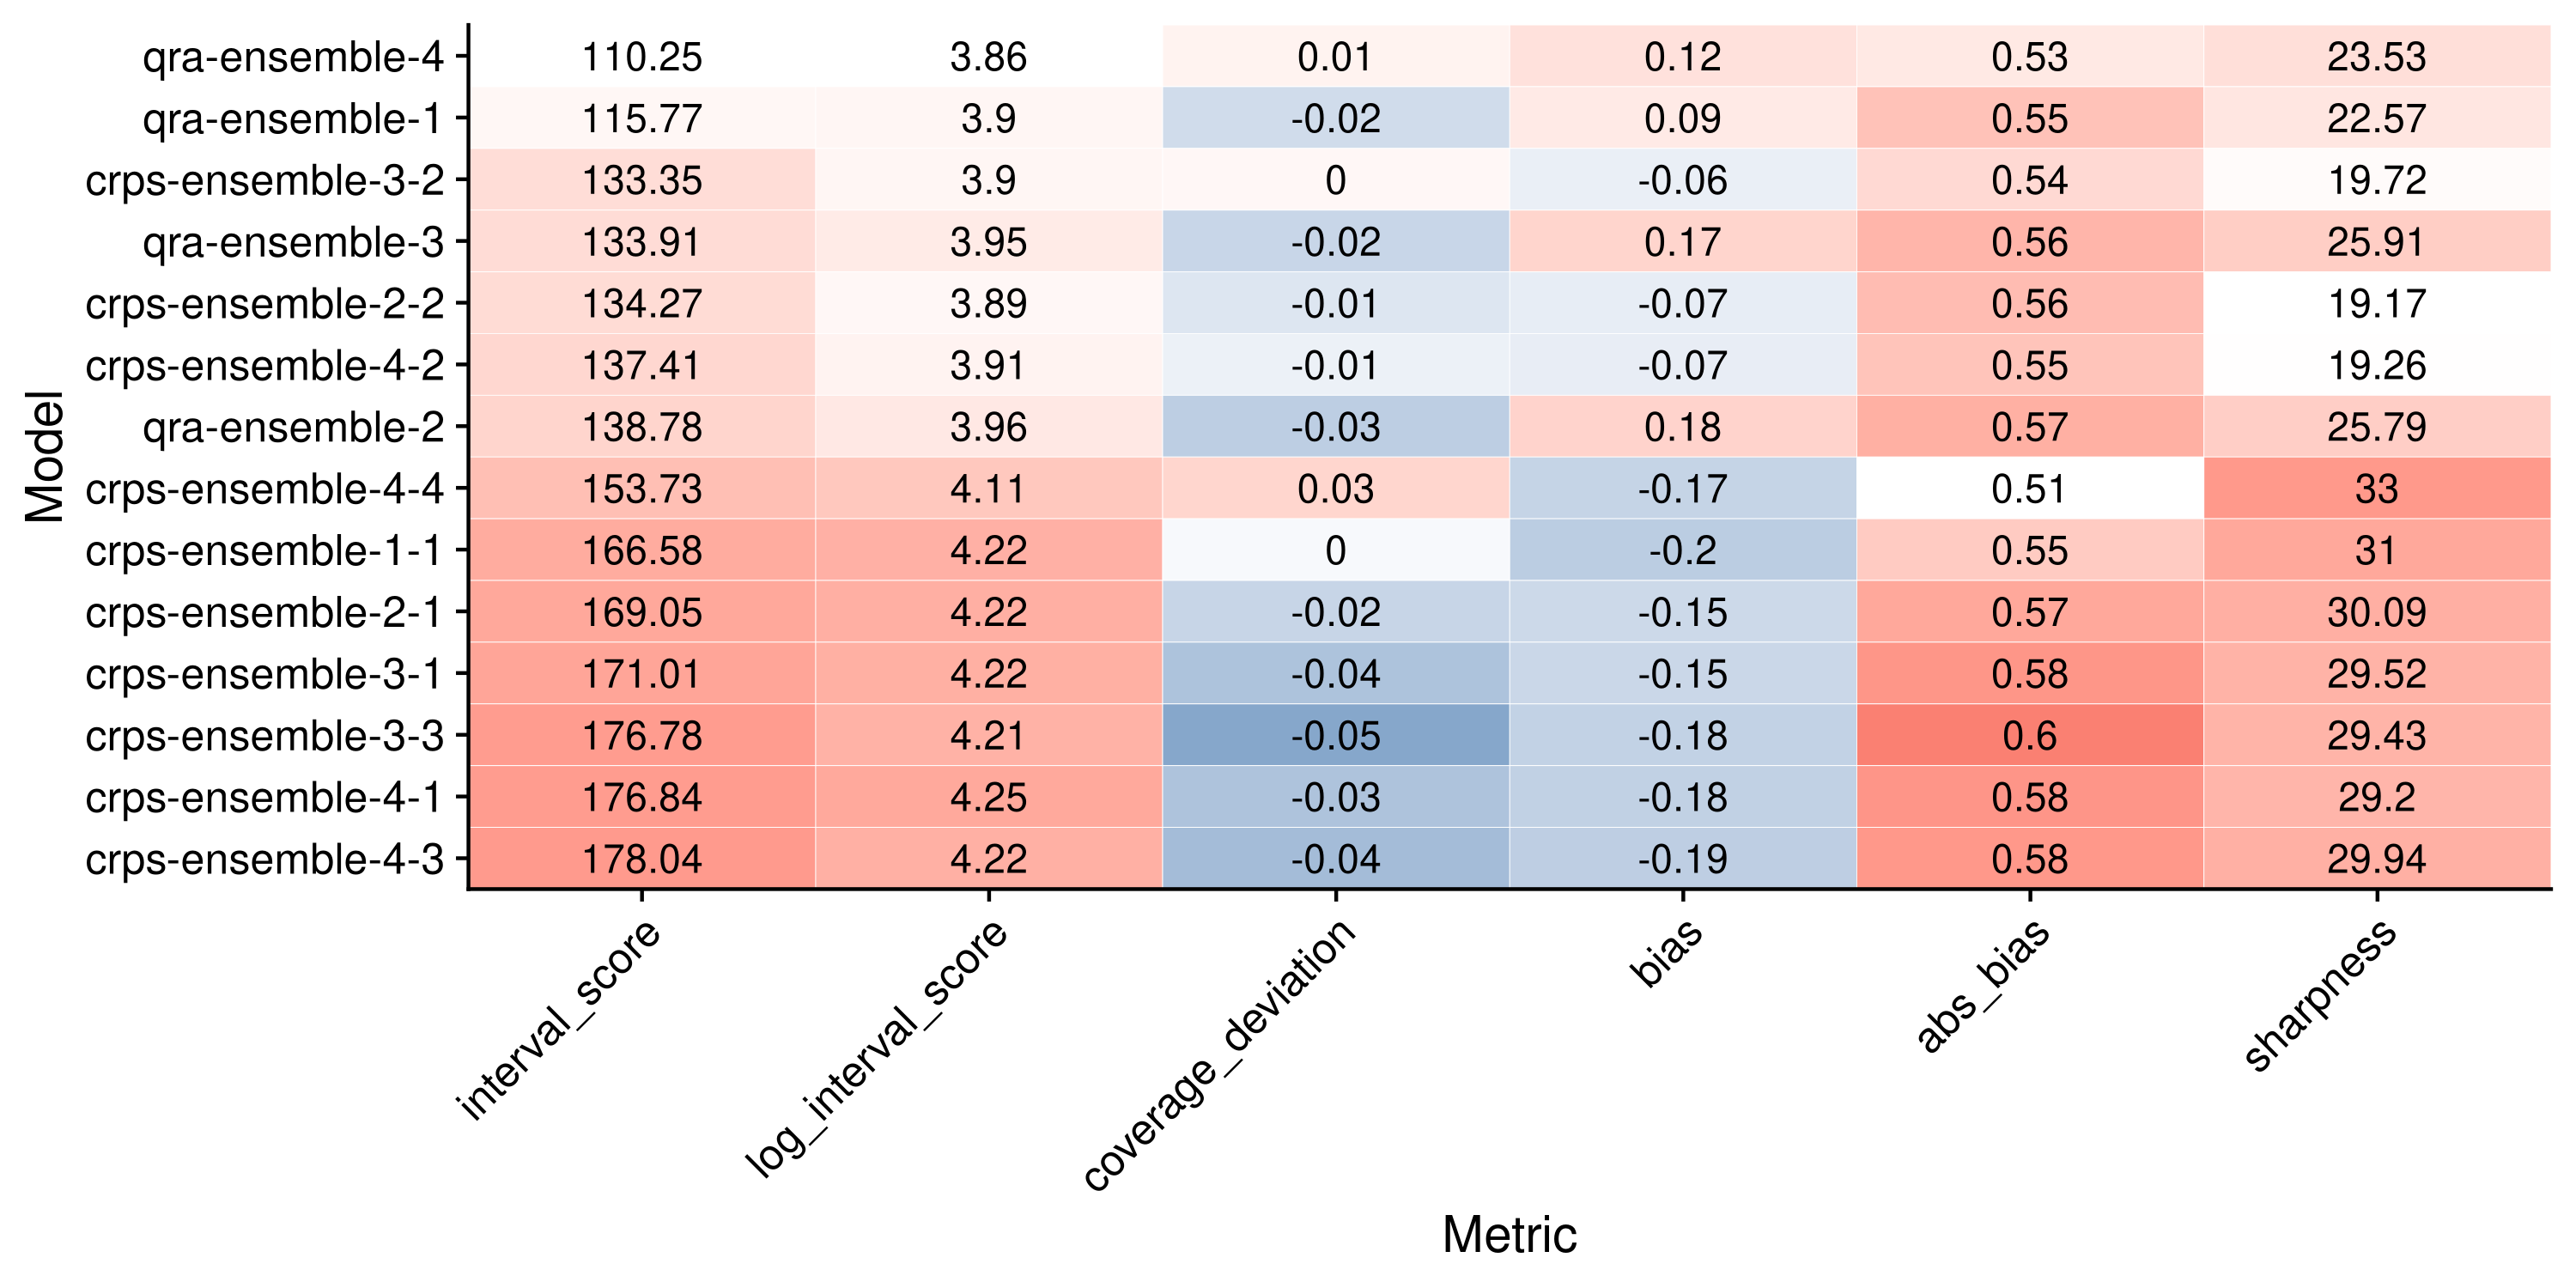
\includegraphics[width=0.5\linewidth]{../visualisation/chapter-5-results/ensembles/scenario-3/coloured-summarised-scores} \caption{Weights given to the different models in the ensemble over time}\label{fig:senitivity-ensembles}
\end{figure}

\hypertarget{discussion-chapter-summary}{%
\section{Discussion / chapter summary}\label{discussion-chapter-summary}}

\begin{itemize}
\tightlist
\item
  Which states were easy to forecast? Which ones were hard to forecast?
\item
  exntension: dealing with missing forecasts
\item
  sensitivity analysis: time included for ensemble weight estimation
\end{itemize}

\hypertarget{discussion}{%
\chapter{Discussion}\label{discussion}}

\begin{itemize}
\item
  crps ensemble works surprisingly well
\item
  tendency bias crps and qra is interesting
\item
  One could argue that the comparison of the ensembles is not entirely fair as the COVIDhub-ensemble model is a much larger ensemble with more components. On the other hand we can require that other ensembles at least not perform worse.
\item
  some riddles can't be answered with the scores: epiforecasts-ensemble1
\item
  this weird perfect correlation
\item
  restriction due to inclusion of the epiforecasts-ensemble1 --\textgreater{} locations and dates
\item
  break up interval score in width part and miss penalty part
\item
  connect bias / coverage deviation more with actually looking at the plots --\textgreater{} when are states hard and easy to forecast?
\item
  More connection between results and model types: which models perform well / badly?
\end{itemize}

  \bibliography{bib/masterthesis.bib,bib/packages.bib}

\end{document}
